\documentclass{osudissert96}

%\usepackage[utf8]{inputenc}
\usepackage[english]{babel}

\usepackage{enumitem,setspace,amssymb,amsmath,graphicx,subcaption}

\usepackage[numbers,sort&compress]{natbib}
\usepackage{notoccite}
\bibliographystyle{unsrtnat}

\usepackage[hidelinks]{hyperref}
\usepackage{doi}

% Macros for consistent formatting
\newcommand*{\fig}[1]{Fig.~\ref{#1}}
\newcommand*{\tab}[1]{Table~\ref{#1}}
\newcommand*{\eq}[1]{Eqn.~\ref{#1}}
\newcommand*{\sect}[1]{\S\ref{#1}}
\newcommand*{\etal}{\textit{et~al}.\ }
\newcommand*{\ie}{\textit{i}.\textit{e}.\ }
\newcommand*{\re}{\mathit{Re}}
\newcommand*{\st}{\mathit{St}}

% Avoid lonely figures
\renewcommand{\topfraction}{0.85}
\renewcommand{\textfraction}{0.1}
\renewcommand{\floatpagefraction}{0.75}

\renewcommand\typesetChapterTitle[1]{#1}

\begin{document}

%
% First, declare the parts of your title page 
%

\author{Michael Crawley}
\title{Understanding the Aeroacoustic Radiation Sources and Mechanism in High-Speed Jets}
\authordegrees{B.S.}  % Degrees thus far, not including this one.
\unit{Department of Mechanical Engineering}

\advisorname{Mo Samimy}
\member{Datta Gaitonde}
\member{James Gregory}
\member{Mei Zhuang}      % Normally you will have advisor + 2 members


%
% The following creates the title page
%

\maketitle
\disscopyright


%
% Abstract goes here.
%

\begin{abstract}
  %  The dissertation abstract can only be 500 words.
It has been well-known within the aeroacoustic community that the dominant noise sources in high-speed turbulent jets are related to the large-scale structures which are generated in the initial shear layer by instabilities and which rapidly grow as they convect downstream.
However, the exact dynamics of these large-scale structures which are relevant to the noise generation process are less clear.
This work represents an attempt to study the dynamics and noise generated by the large-scale structures quantitatively and in high-fidelity in a Mach 0.9 turbulent jet using simultaneous pressure and velocity data acquisition systems alongside plasma-based excitation to produce coherent ring vortices in the shear layer.

In the first phase, the irrotational near-field pressure is decomposed into its constitutive acoustic and hydrodynamic components, and two-point cross-correlations are used between the acoustic near-field and far-field in order to identify the dominant noise source region.
Building upon the work of previous researchers, the decomposition is performed using a spatio-temporal wavelet transform, which was found to be more robust than previous algorithms.
Results indicated that for both individual as well as periodic large-scale structures, the dominant noise source region constitutes the upstream region of the jet, ending just before of the end of the potential core (in a time-averaged sense) in the unexcited jet.

The large-scale structure interactions were then investigated by stochastically-estimating the time-resolved velocity fields from the time-resolved near-field pressure.
For computational efficiency, the ensemble velocity snapshots were first decomposed into orthogonal modes, and the a mapping from the near-field pressure to the expansion coefficients was then produced using a feedforward neural network using backpropagation for learning.
The coherent structures generated by the excitation were then identified and tracked using standard vortex identification routines.
For the impulsively-excited jet, the individual structures quickly rolled up into a coherent structure within two jet diameters and then advected until roughly four jet diameters downstream, at which point it underwent a rapid disintegration.
For the periodically-excited jet, multiple smaller-scale structures are initially produced; these quickly merge into a single large-scale structure which matches the excitation wavelength.
Similar to the impulsively-excited structures, these now large-scale structures advect downstream and undergo a rapid disintegration near the end of the potential core. 

Finally, from Ribner's dilatation-based acoustic analogy the aeroacoustic source terms were computed using the time-resolved velocity field produced by the stochastic estimation.
Interpretation of the results is limited however, due to the number of assumptions and simplifications necessary for the computations, given the realities of the available experimental facilities.
Analysis of the computed source fields identified the coherent structures producing a convected wavepacket-like event, centered on the jet lipline though reaching into the potential core.
For the individual vortex rings, a clear modulation of the spatial extent and amplitude was observed as the vortex began to break down just upstream of the end of the potential core.
This behavior is also present for the periodic train of vortices, however it is obscured by an amplification of the source in the upstream region, corresponding to the pairing location for the multiple smaller-scale structures generated by the excitation. 



\end{abstract}

\dedication{I would like to dedicate this work to Dr. Rachelle Speth, for her tireless efforts to convince me to hurry up and graduate already. Also, my parents.}


%
% Bring in Acknowledgement and Vita from separate files named ``ack.tex''
% and ``vita.tex''.
%

\begin{acknowledgements}
I should probably acknowledge someone here \ldots
\end{acknowledgements}


\begin{vita}

\dateitem{September 10, 1986}{Born - Plano, Texas}

\dateitem{2009}{B.S. Mechanical Engineering, \\
				University of Texas, Austin.}

\dateitem{2009-present}{Graduate Research Associate,\\
			 The Ohio State University.}


\begin{publist}

%% UPDATE FOR 2010:
%  Grad school only wants research publications, and it only wants those
%  research pubs that are actually published. Accepted or ``to appear''
%  publications don't count. If they look closely, they'll tell you to
%  remove any publications that aren't in print. Haivng said that, they
%  probably won't look that closely unless you put a really long list
%  here. You're tempting fate if you add instructional publications
%  though.

\researchpubs

\pubitem{\textbf{M. Crawley}, C.-W. Kuo, and M. Samimy,
\newblock ``Identification of the Acoustic Response in the Irrotational Near-field of an Excited Subsonic Jet.''
\newblock submitted to \emph{International Journal of Aeroacoustics}.}
	

\pubitem{\textbf{M. Crawley}, R. Speth, D. V. Gaitonde, and M. Samimy, 
\newblock ``A Study of the Noise Source Mechanisms in an Excited Mach 0.9 Jet - Complementary Experimental and Computational Analysis.''
\newblock AIAA Paper 2015-0736, \emph{53$^{rd}$ AIAA Aerospace Sciences Meeting}.}
	

\pubitem{\textbf{M. Crawley}, A. Sinha, and M. Samimy, 
\newblock ``Near-field and Acoustic Far-field Response of a High-Speed Jet Forced with Plasma Actuators.''
\newblock \emph{AIAA Journal}, expected 2015.}
	

\pubitem{\textbf{M. Crawley} and M. Samimy, 
\newblock ``Decomposition of the Near-Field Pressure in an Excited Subsonic Jet.''
\newblock AIAA Paper 2014-2342, \emph{20$^{th}$ AIAA/CEAS Aeroacoustics Conference}.}
	

\pubitem{\textbf{M. Crawley}, A. Sinha, and M. Samimy, 
\newblock ``Near-field Pressure and Far-field Acoustic Response of Forced High-Speed Jets.''
\newblock AIAA Paper 2014-0527, \emph{52$^{nd}$ AIAA Aerospace Sciences Meeting}.}	
	

\pubitem{\textbf{M. Crawley}, H. Alkandry, A. Sinha, and M. Samimy, 
\newblock ``Correlation of Irrotational Near-Field Pressure and Far-Field Acoustic in Forced High-Speed Jets.''
\newblock AIAA Paper 2013-2188, \emph{19$^{th}$ AIAA/CEAS Aeroacoustics Conference}.}
	

\pubitem{H. Alkandry, \textbf{M. Crawley}, A. Sinha, M. Kearney-Fischer, and M. Samimy,
\newblock ``An Investigation of the Irrotational Near Field of an Excited High-Speed Jet.''
\newblock AIAA Paper 2013-0325, \emph{51$^{st}$ AIAA Aerospace Sciences Meeting}.}
	

\pubitem{\textbf{M. Crawley}, M. Kearney-Fischer, and M. Samimy, 
\newblock ``Control of a Supersonic Rectangular Jet Using Plasma Actuators.''
\newblock AIAA Paper 2012-2211, \emph{18$^{th}$ AIAA/CEAS Aeroacoustics Conference}.}
\end{publist}



\begin{fieldsstudy}

% The \majorfield* uses the unit specified in the \unit command used
% earlier in your document. If you want to use a different unit, use the
% second form shown here
%\majorfield*
\majorfield{Mechanical and Aerospace Engineering}

%%
%% Note:  If there were only one field of study, the following list 
%%        would best be done using the following command:
%%
%%  \onestudy{Only Topic}{Only Professor}
%%

% \begin{studieslist}
% \studyitem{Topic 1}{Prof.\ Big Dude}
% \studyitem{Topic 2}{Prof.\ Other Dude}
% \studyitem{Topic 3}{Prof.\ Another Dude}
% \end{studieslist}

\end{fieldsstudy}

\end{vita}




%
% Make the Table of Contents and other good stuff
%

\tableofcontents
\listoftables
\listoffigures


%
% The following is a list of chapters.  Each is brought in from a
% separate file using the \include{} command.
%

\chapter{Introduction}
\label{introduction}
\section{Motivation}
The advent of the turbojet engine led to a transformation in both commercial and military aviation, allowing for much faster flight than previously possible with propellor-driven aircraft. 
However, the increased thrust of turbojets has come at great cost; significant acoustic radiation is generated by the rotating components (compressor, turbine, fan), by the combustion process, and ultimately by the free jet itself. 
On the commercial side, the escalating number of flights, encroachment of urban and residential areas near airports, and tightening of environmental regulations have combined to force airports to institute curfews, surcharges and flight path restrictions to combat noise pollution. 
For the military, hearing damage inflicted on nearby personnel (particularly flight deck crew on aircraft carriers) has necessitated the implementation of noise reduction concepts on tactical aircraft.
During takeoff and landing, when acoustic radiation is most problematic to ground crew and  surrounding urban and residential areas, the dominant noise source of the jet engine is the aeroacoustic radiation generated by the high velocity engine exhaust.
This has spurred extensive research, spanning over six decades, into the acoustic source mechanism in high speed, high Reynolds number jets. 

While progress has been made in the field of aeroacoustics, both experimentally \citep{Tam1996, Viswanathan2006, Tam2008} as well as theoretically \citep{Cabana2008}, understanding of jet noise sources and their radiation mechanisms remains incomplete \citep{Jordan2008}.
This is due to the large number of interrelated parameters (e.g. Reynolds number, temperature ratio, acoustic Mach number, nozzle geometry, et cetera) as well as the large disparity in the associated length and time scales of the turbulent phenomena and the radiated noise.
Simulations of controlled free shear layers have suggested that there is significant potential for noise reduction, on the order of 11 dB in some cases [Wei 2006].
However, these simulations relied on non-physically defined actuation (that is, forcing was applied over a defined region by arbitrary energy, momentum, and body force terms), and a physical interpretation of the optimum forcing parameters was not immediately clear to the researchers.
Current noise-mitigation technologies for free jets have largely been applied in an adhoc fashion, due to our incomplete understanding of the aeroacoustic sources.
Fully realizing this maximum noise reduction potential will require a much more detailed understanding of the mechanism (or mechanisms) by which free jets radiate to the far-field.

It is generally agreed that the dominant noise sources are related to the large-scale turbulent structures present in the mixing layer of the jet. 
What remains to be determined is what aspects of the large-scale structure evolution and interactions are relevant to the noise generation process. 
Theoretical models of spatially- and temporally-modulated coherent structures have shown great promise in replicating the observed characteristics of the dominant far-field noise [Cavalieri/Jordan?]. 
However, direct experimental data linking this structure evolution to the acoustic emission is still lacking. 
It is on this vein that the current work is focused.
Until recently, experimental data acquisition techniques have been unable to capture the flow physics with enough fidelity (lacking in either spatial or temporal resolution) in order to accurately model the large-scale structures and aeroacoustic sources.
By combining contemporary data acquisition methods (free-field microphones and non-time-resolved particle image velocimetry) with novel post-processing algorithms this work aims to directly link the relevant vortex dynamics of the large-scale structures to the acoustic emission events, and in the process identify a simplified aeroacoustic source mechanism. 

This study can be broken down into three distinct parts. 
In the first, the irrotational near-field and acoustic far-field of the jet is analyzed in order to identify the dominant acoustic source region.
In the second, time-resolved velocity fields are estimated using an artificial neural network, which is trained to generate a mapping from time-resolved pressure measurements to instantaneous velocity.
Lastly, the acoustic source is computed from the time-resolved velocity using Ribner's simplification of Lighthill's acoustic analogy.  
	
\section{Background}
\subsection{Flow Control}
\label{sec:flow_instabilities}
Controlling the development of the jet plume, and hence controlling the rate of mixing or intensity and characteristics of the emitted acoustic radiation, is a long running goal of the aeroacoustic community.
Passive, permanent modifications to the nozzle have been shown to be quite adept at this task; some examples of these include tabs [citations] and chevrons [citations]. 
These work to generate counter-rotating streamwise vortices in the developing shear layer, which serve to substantially increase mixing between the core and coflow in the near-nozzle region and ultimately retard the growth of large-scale axisymmetric structures [citation].

Unfortunately, these passive modifications have associated penalties to the engine performance, in terms of added weight or reduced thrust.
Due to the passive nature of the flow modification, these performance penalties are in effect over the entire duration of the flight regardless of whether or not the noise reduction is needed. 
To improve engine efficiency, active control techniques are desired, since they can be activated when needed, such as during takeoff and landing, and deactivated when unneeded, such as after a commercial airliner reaches cruising altitude. 
Active control techniques, which seek to manipulate instabilities in the jet shear layer, have been extensively studied in low-speed, low-Reynolds number jets, the most common of which is acoustic drivers [citations]. 
However, as the speed and Reynolds number of the jet is increased (to match those in practical applications), so too does the required bandwidth and energy of the active drivers. 
Hence, acoustic or magneto-hydrodynamic drivers lose control authority in these regimes, and more powerful actuators are required.

The last decade has seen a rapid growth in the development of plasma actuators for use in high-speed flow control; though as of yet they have not progressed past the experimental phase.
Localized arc filament plasma actuators (LAFPAs) are one such class of plasma actuator, which were developed by a collaboration between the Gas Dynamics and Turbulence Laboratory (GDTL) and the Non-Equilibrium Thermodynamics Laboratory (NETL) at the Ohio State University.
LAFPAs can provide the high-amplitude and high-frequency excitation required for control of high Mach number and high Reynolds number jets [citations]. 
GDTL has used these actuators for noise mitigation and flow control in Mach 0.9 [citations], Mach 1.3 [citations] and Mach 1.65 [citations] jets (both heated and unheated). 
A review of the development of LAFPAs and their use in flow control and fluid phenomena research in high speed, high Reynolds number jets can be found in Samimy et al. [citation]. 
More recently, the diagnostic potential of LAFPAs for understanding jet flow phenomena has been explored. Excitation of instabilities in the flow by LAFPAs results in a definitive spatio-temporal origin to which resulting phenomena can be referenced. 
The absolute temporal reference afforded by LAFPA excitation provides researchers the ability to investigate the growth, saturation, and decay of structures with high fidelity. 
An example of their diagnostic potential can be found in the work of Kearney-Fischer \etal [citation], which investigated Mach wave radiation from heated, high Mach number jets using schlieren imaging phase-locked to LAFPAs. 

Unlike their passive counterparts (such as tabs or mechanical chevrons), or some other potential active flow control technologies (such as fluidic chevrons), LAFPAs control the shear layer development indirectly by exciting naturally occurring instabilities.
The sharp velocity gradient in the jet shear layer (or, more precisely the inflection point produced by this sharp gradient) gives rise to the inviscid Kelvin-Helmholtz instability [citation] (sometimes simply referred to as the initial shear layer instability).
This instability is broadband and scales with the local momentum layer thickness and jet exit velocity ($\theta / U_j$) ; perturbations over a wide range of frequencies can be amplified, though the dominant frequencies are found to be on the order of $St_{\theta} = f \theta /U_j = 0.012$ for very thin boundary layers [Cohen and Wygnasnki?]. 
The Kelvin-Helmholtz instability then drives the development of the large-scale structures in the shear layer by amplifying fine-scale perturbations, ultimately causing them to roll-up into coherent structures regardless of Reynolds number [Crow and Champaign, Brown and Roschko].
Owing to the axisymmetry of the jet nozzle (i.e. that the initial shear layer wraps around and connects to itself), various azimuthal Fourier modes are unstable to perturbations (including both axisymmetric and higher order modes) [Cohen?].

The growth of the shear layer as it advects downstream ultimately dictates that the shear layer merges with itself; this location is referred to as the end of the potential core.
A secondary instability, the jet column instability, manifests in axisymmetric jets and is related to the passage of large-scale structures through the end of the potential core.
This instability scales with the jet exit diameter and jet exit velocity ($D / U_j$) and is broadband, with a dominant characteristic frequency of $St_{D} = f D /U_j = 0.3$.
The relation of the jet column instability to the initial shear layer instability is not well understood.  
Kibens argued that the jet preferred frequency is related to the initial shear layer frequency by the number of pairings of large scale structures that occur before the end of the potential core (i.e. $f_n / f_p = 2^n$), as the frequency of the structures halves after each pairing process [Kibens].  
Conversely, Petersen claims that the jet preferred mode is simply the initial shear layer instability at the end of the potential core, and that the appearance of a single dominant lengthscale for the axisymmetric mode is due not to a type of `global' instability of the flow field, but to a cutoff at the end of the potential core of the axisymmetric instability [Petersen and Samet 1988].
Regardless, it is clear that the large-scale oscillations of the jet shear layer and potential core are ultimately the product of small-scale perturbations which are amplified by the initial shear layer instability.

LAFPAs achieve flow control by utilizing this relationship between the initial shear layer instability and the jet column instability.
The localized plasma arc-filament produces a rapid, localized heating through the Joule effect, and a compression wave is formed [Utkin 2007].
Though these perturbations are spatially discrete, they quickly amplify into large-scale coherent structures with well-defined characteristic spatial, temporal, and azimuthal frequencies.
Thus, LAFPAs are able to control the development of the most energetic scales in the jet shear layer; large-scale, azimuthally-coherent structures can be generated when enhanced mixing and jet spreading are desired, or smaller-scale, less azimuthally-coherent structures when noise reduction is necessary. 
In the present work, the subsonic jet is excited by LAFPAs, though here the goal is diagnostic rather than immediate practical application.
The well-defined frequencies and phase of the large-scale structures produced by LAFPA actuation serve as an excellent reference for data acquisition and post-processing (e.g. phase-locking and phase-averaging).

\subsection{Lighthill's Acoustic Analogy}
Far outside the jet, where the medium is quiescent, no sources or sinks are present, and any disturbances are low-amplitude and isentropic, the governing equations can be linearized and simply reduced to a homogeneous wave equation
\begin{equation}
	\frac{\partial^2 p}{\partial t^2} - c^2 \nabla ^2 p = 0
\end{equation}
which describes the non-dispersive propagation of (acoustic) waves through space and time.
Lighthill \citep{Lighthill1952} was the first to identify that the governing equations for fluid dynamics could also be rearranged in such a manner as to produce a propagating wave equation \textit{inside the jet}.
Prior to this, aeroacoustic studies had observed that the frequency content of the far acoustic field matched that of the flow field, but had not identified a way to estimate the acoustic intensity.

Starting with the conservation of mass and momentum equations, one can take the divergence of the former and the partial derivative with respect to time of the latter, and combine these along with the equation of state to produce
\begin{equation}
\frac{1}{c^2}\frac{\partial^2 p}{\partial t^2} - \nabla^2 p = \nabla \cdot \nabla \cdot \mathbf{T}.
\end{equation}
$\mathbf{T}$, commonly referred to as \textit{Lighthill's stress tensor}, comprises Reynolds stresses, viscous stresses, and entropy fluctuations, respectively:
\begin{equation}
\mathbf{T} = \rho \mathbf{u} \otimes \mathbf{u} - \mathbf{\tau} + \mathbf{I} \left[ (p-\bar{p}) - c^2 (\rho - \bar{\rho}) \right].
\end{equation}
Here, $c$ refers to the ambient speed of sound, $\mathbf{I}$ is the identity matrix, $\mathbf{\tau}$ is the shear stress tensor, and an overbar ($\bar{\cdot}$) corresponds to a time-averaged quantity.
This transformation has the effect of approximating the real system as a uniform acoustic medium at rest which is being driven by an external fluctuating force field.
As the wave operator is linear, the solution to this equation can be formulated with the aid of Green's functions,
\begin{eqnarray}
\frac{\partial^2 G}{\partial t^2} - c^2 \nabla^2 G = \delta (\tau -t) \delta (\mathbf{x}' - \mathbf{x}).
\end{eqnarray}
The solution to this (see Crighton \etal [cite]) is the deceptively simple spatial integration of the source field at retarded time (that is, it is accounting for the propagation delay from the source location to the observer):
\begin{equation}
p (\mathbf{x},t) = \frac{1}{4 \pi c^2} \nabla \cdot \nabla \cdot \int_{\Omega} \frac{\mathbf{T} (\mathbf{x}',t - |\mathbf{x} - \mathbf{x}'|/c)}{|\mathbf{x} - \mathbf{x}'|} d^3 \mathbf{x}'.
\end{equation}

Lighthill's derivation of what became known as the first acoustic analogy (which in fact was specifically tailored to the study of jet noise) reformed the study of aeroacoustics.
As has been discussed by many authors before (see Goldstein 1974 for example), this equation describes the propagation of sound, through a quiescent medium, generated by quadrupole sources. There have been several major assumptions made in this derivation, that the flow is completely subsonic (and hence no shock or expansion waves are present), that the observer location is far from the jet (and hence hydrodynamic pressure fluctuations or `pseudo-sound' is negligible), that there are no solid boundaries near the flow (and hence, no reflections, diffraction, absorption, or scattering) and finally that the acoustic waves themselves do not act as sources as they propagate through the flow.
Nonetheless, this theoretical framework is still applicable to a wide variety of commercial and scientific inquiries, present study included.

Theoretical work based on Lighthill's approach was successful in predicting some aspects of experimentally-observed jet noise.
Namely, stochastic source models of quadrupoles (per the aeroacoustic community's understanding of jet turbulence at the time) predicted a far-field pressure intensity scaling of $I \sim U_{j}^{8}$ which agreed with experimental results from cold, subsonic jets at sideline angles [Viswanathan].
However, this scaling law does not hold when the jet is heated, necessitating more complex source models. 
Unfortunately, given the complexity of the source field, even modern experimental techniques cannot acquire the full source with sufficient spatial and temporal fidelity to elucidate the flow structures responsible for the dominant noise emission.

Later researchers further refined Lighthill's approach (e.g. Howe [cite], Goldstein [cite] and Lilley [cite]); providing successively clearer characterizations of the source physics.
In addition to the true noise sources, Lighthill's acoustic source term includes flow-acoustic interactions, which describe diffraction and convection effects rather than true sources of noise, and which these researchers have attempted to separate from the true noise sources.
Alternative acoustic analogies have also been proposed, such as Powell's theory of vortex sound [cite] and Doak's momentum potential theory [cite].
In a slightly different vein, analytical decompositions have been performed in order to separate the disparate fluid phenomena inherent in Lighthill's source term and identify the roles of each [cabana 2008].
In each of these theories however, the source field for a high-speed, turbulent jet is highly complex and defies a simple physical understanding of the dynamical processes which lead to the noise emission.   

\subsection{The Role of Large-Scale Structures}
Initial understanding of turbulence was that it was stochastic in nature - that the frequency and appearance of turbulent eddies in a flow was random, with little to no prescribed preference.
It was in this context that Lighthill's acoustic analogy was first developed, and as a result initial models for the source field assumed a stochastic distribution of quadrupoles.
This source model was shown to produce an intensity which scaled with the eighth-power of the flow velocity, which was in general agreement with the experimentally-observed intensity scaling of cold, subsonic jets [Lighthill 1954].
The downstream convection of these quadrupoles produces a preferential directivity in the emitted acoustic radiation, with a maximum predicted to occur near 45$^\circ$ from the jet axis, again in general agreement of experimental far-field spectra [Lighthill 1954].
However, researchers have found that stochastic quadrupole source models fail to accurately predict the intensity scaling of jet noise in heated jets or cold jets at low observer angles [Tam 2008].
As Lighthill's analogy is an exact rearrangement of the governing equations (aside from the relatively minor assumption of a constant speed of sound), the error lies in our understanding of the aeroacoustic source. 

Mollo-Christensen [cite], and later Crow \& Champagne [cite] and Brown \& Roshko [cite], were the first to identified large-scale, coherent vortical structures underpinning turbulent free shear layers, in addition to the fine-scale, stochastic eddies.
Later researchers linked the appearance of these large-scale structures to natural flow instabilities (predominantly the Kelvin-Helmholtz instability discussed in \sect{sec:flow_instabilities}) [Michalke, Cohen and Wygnanski].
Following the identification these coherent structures in turbulent jet shear layers, source term models based on large-scale eddies have frequently been employed, to varying degrees of success. 

A simplified model of the noise generation process in stationary free jets can be found in \fig{fig:jet_sources_diagram}. 
This model is from the work of Tam \etal \citep{Tam1996, Tam2008}, who observed that the far-field spectra could be represented as a combination of two similarity spectra based on polar angle of the observer, regardless of jet Mach number or temperature.
At observer angles close to the jet downstream axis, the spectra exhibited a clearly defined spectral peak (\emph{F}-spectrum), whereas at sideline or upstream angles the spectra were broadband (\emph{G}-spectrum).
From this observation the two-component acoustic source model was born: the isotropic fine-scale turbulence, dominant in the near-nozzle region, is responsible for the omni-directional acoustic radiation that dominates the sideline and upstream polar angles. 
On the other hand, the large-scale turbulent structures which exist further downstream produce the superdirective radiation that is readily apparent at aft polar angles. 
This model of large-scale (and to a lesser extent fine-scale) turbulence noise generation explains the so-called 'mixing noise' generated by both subsonic and supersonic jets.
\begin{figure}
	\centering
	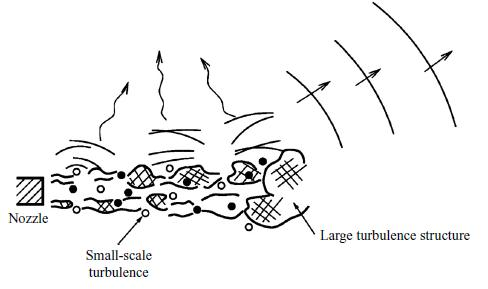
\includegraphics[width=5in]{Figures/JetNoiseSourceDiagramTMP.jpg}
	\caption{Simplified diagram of jet noise sources, reprinted from Tam \etal JFM 2008.}
	\label{fig:jet_sources_diagram}
\end{figure}
Numerous experimental studies have lent credibility to this view of aeroacoustic noise generation; see for example, Panda \etal [cite], Viswanathan \etal [cite], Tam \etal [cite], and Bogey \& Bailley [cite 2005].
There is little disagreement at this point that the large-scale coherent structures in the turbulent shear layer are responsible for the dominant noise emission; however, the exact dynamics of these which leads to acoustic emission are as of yet still not well-understood. 

[Wavepacket models???]
 
Additional noise source mechanisms have been identified for supersonic jets. In imperfectly expanded jets, shock cells are produced in the jet. As turbulent structures pass through these waves, the sharp pressure gradients cause them to emit acoustic radiation. 
This is observed directly in the far-field as a broad-band amplification at high frequencies, referred to simply as broad-band shock-associated noise (BBSAN). 
In stationary or subsonic airframes this radiation can generate a feedback loop, whereby the noise travels upstream to the nozzle exit, excites the initial shear layer, and produces new structures at the same frequency.
A high-amplitude, narrow-band tone (screech noise) is the end result of this feedback loop.
Lastly, supersonically-convecting (relative to the ambient) large-scale structures (which exist in supersonic and heated jets) produce high-amplitude, strongly-directional acoustic radiation towards aft angles.
This Mach wave radiation can be explained by a wavy-wall analogy [Tam].
In the present work, the jet is unheated and subsonic; as such these noise sources are not present and therefore neglected throughout the rest of this work.

        
\chapter{Experimental Methodology}
\label{methodology}

\section{Anechoic Chamber}
All experiments were conducted at the GDTL within the Aerospace Research Center at the Ohio State University. 
Compressed, dried, and filtered air is supplied to the facility from two cylindrical storage tanks with a total capacity of 43 m$^{3}$ and maximum storage pressure of 16 MPa.
The air may be routed through a storage heater (not used in this study), which allows the jet to operate with a stagnation temperature up to 500 C, before expanding through a nozzle and exhausting horizontally into an anechoic chamber. 
Opposite the nozzle, a collector accumulates the jet and entrained air and exhausts to the outdoors. 
A schematic of the anechoic chamber can be seen in \fig{fig:chamber}. 
The dimensions of the chamber are 6.20 m wide by 5.59 m long and 3.36 m tall, with internal wedge-tip to wedge-tip dimensions of 5.14 m by 4.48 m and 2.53 m, respectively. 
The design of the chamber produces a cutoff frequency of 160 Hz, below the frequencies of interest for this study. 
A more detailed description of the GDTL anechoic chamber properties and validation has been given by [Hahn?].
\begin{figure}
	\centering
	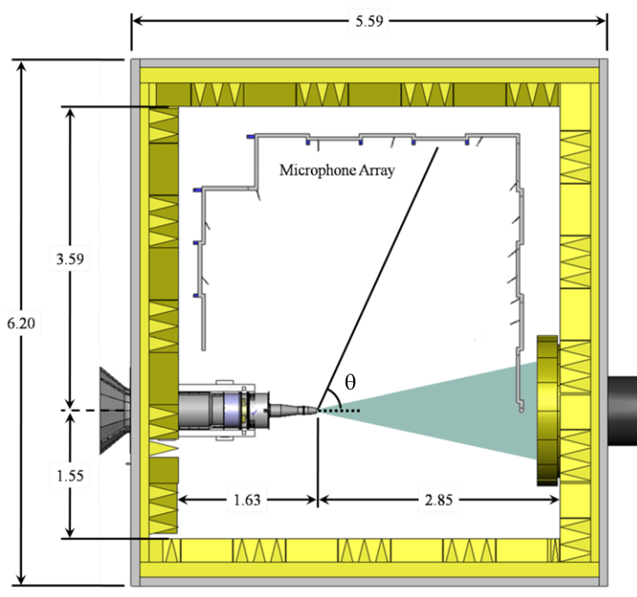
\includegraphics{Figures/Chamber_Schematic.png}
	\caption{Top-down view of anechoic chamber and free jet facility at GDTL; dimensions are in meters.} 
	\label{fig:chamber}
\end{figure}

For this study a converging, axisymmetric nozzle with exit diameter D of 25.4 mm was used. 
The internal contour of the nozzle was designed using a fifth order polynomial. 
The nozzle utilized a thick-lipped design in order to simplify the mounts for the LAFPA extension, which housed the eight actuators used in this study. 
For the experiments reported in this paper, the jet was operated at a Mach number ($M_j$) of 0.90, and with a total temperature ratio of approximately unity. 
The Reynolds number based on the jet exit diameter was $6.2\times〖10〗^5$; previous investigations using hot-wire anemometry have indicated that the initial shear layer is turbulent for this operating condition with momentum thickness ~0.09 mm and boundary layer thickness ~1 mm [Kearney?].

\section{Localized Arc-Filament Plasma Actuators}
The design of the localized arc-filament plasma actuators, as well as the driving circuitry, has undergone a slow evolution since their initial development by the GDTL and NETL.
In the current work, each LAFPA actuator consists of a pair of 1~mm diameter tungsten pin electrodes.
The center-to-center spacing between electrode pairs for each actuator is 4 mm.
Eight actuators were uniformly spaced around the nozzle perimeter 1 mm upstream of the nozzle exit. 
For electrical and thermal durability, the electrodes were housed in a boron nitride (grade AX05) extension attached to the end of the nozzle. 
A groove with dimensions of 1 mm wide and 0.5 mm deep is machined in the boron nitride, into which the electrode tips protrude, to provide a region of low momentum flow in order to stabilize the plasma arcs. 
It has been shown that the existence of this groove does not substantially alter the flow field or the control authority of the LAFPAs [citation]. 
A detailed description of initial development and LAFPA characteristics can be found in Utkin et al. [citation].

The LAFPAs were energized by a multi-channel, high-voltage plasma power generator ()capable of simultaneously powering up to eight LAFPAs), which was designed and built in-house at the GDTL. 
In the second-generation power supply, each individual circuit consists of a switchable capacitor in line with a high voltage transformer; the arcing electrodes are connected to the secondary side of the coil. 
The capacitor is charged by a 100 V DC power supply when the first switch is closed and the second is opened; at the user-specified time the switches flip and it discharges through the coil. 
The switches are controlled by a 16-channel digital I/O card and National Instruments' Labview software, operated by a dedicated computer. The plasma generator provides independent control of the frequency, duty cycle/pulse width, and phase of each individual actuator (though not the amplitude). 
The pulse width was held constant at 7 μs, which was found to be the minimum pulse width at which the actuators consistently arced for all frequencies explored in this study [citation]. 
The circuit is limited to 20 kHz due to thermal concerns.
However, as the current work is focused on the evolution of large-scale structures (and ultimately their acoustic radiation), this is not an issue.

\section{Data Acquisition}
\subsection{Near- and Far-field Pressure}
Near-field and far-field pressure measurements were acquired using Brüel \& Kjær ¼ inch 4939 microphones and preamplifiers. 
The signal from each microphone is band-pass filtered from 20 Hz to 100 kHz using a Brüel \& Kjær Nexus 2690 conditioning amplifier, and recorded using National Instruments PXI-6133 A/D boards and LabVIEW software. 
The microphones are calibrated using a Brüel \& Kjaer 114 dB, 1 kHz sine wave generator (model \# ???). 
The frequency response of the microphones is flat up to roughly 80 kHz, with the protective grid covers removed. 

Far-field acoustic pressure is acquired at three polar angles: 30°, 60° and 90°, as measured from the downstream jet axis. 
The positioning of the far-field microphone array can be seen in \fig{fig:chamber}.
The microphones were oriented such that they are at normal incidence to the jet downstream axis at the nozzle exit. 
The radial distance of the microphones ranges from 101D at 30° to 145D at 60°. 

The near-field pressure was acquired  during two separate experimental campaigns; the first focusing purely on the near-field and far-field pressure and the second focusing on the instantaneous velocity field. During the first campaign, the irrotational near-field was acquired using a linear array of sixteen microphones located along the meridional plane of the jet; the spacing varied along the array from 1D to 2D \fig{nearfield1_schematic}. 
The array was mounted on an x-y linear traverse system the array and was inclined at an angle of 8.6º to the jet axis in order to match the spreading angle of the jet shear layer, as determined via PIV measurements during previous studies [28]. 
The traverse was controlled using LabView and enabled the acquisition of pressure measurements at various radial positions with respect to the jet axis. 
Initially, the most upstream microphone is positioned at x/D = 1 and r/D = 1.20, which is just outside the initial shear layer.
For subsequent cases, the microphone array was incremented radially outward by 0.5D for a total travel distance of 7D, for a total of 15 array locations in the radial direction.
Voltage signals were collected at 200 kHz with 81920 data points per block; sub-blocks of 8192 data points were used when calculating short-time power spectral densities, resulting in a frequency resolution of 24.4 Hz. 
Ten blocks were recorded for each case resulting in four seconds of data, which has been found to be sufficient for statistical convergence.
\begin{figure}
	\centering
	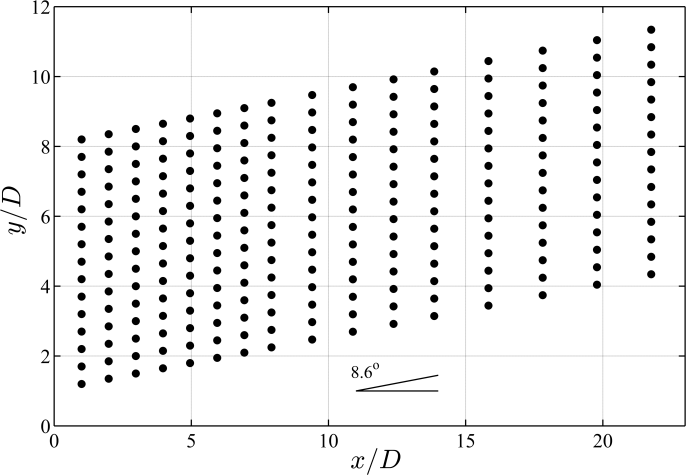
\includegraphics{Figures/NearField1_Schematic.png}
	\caption{Schematic of the microphone positions ???}
	\label{nearfield1_schematic}
\end{figure}

In the second experimental campaign, a shorter array consisting of 12 microphones equally space by $1D$ was used. 
In this case, the array was mounted from the floor and at an angle off the meridional plane of the jet (with microphone tips angled normal to the jet axis).
This setup was used in conjunction with the particle image velocimetry described in the following section; the microphone array was placed off of the meridional plane so that it did not intersect with the laser sheet. 
As before, the microphone array was angled 8.6º with respect to the jet axis in order to match the spreading rate of the shear layer, and the axial and radial position was set to match the closest microphone array location used during the first experimental campaign.
Voltage traces were acquired at 400 kHz, with 24576 points collected per block.
The voltage traces were collected simultaneously with streamwise particle image velocimetry measurements (described in the following section); 1500 blocks were acquired, corresponding to the 1500 acquired images.

In addition to the microphone voltage traces, the acoustics data acquisition system recorded a reference signal corresponding to the LAFPA excitation. 
The TTL pulse sequence, which controls the LAFPAs, was supplied to an Agilent 3320A waveform generator. 
The rising edge of the TTL pulse triggered a sharp drop in the output voltage of the waveform generator, which then ramps back up to the original voltage over a time interval which is shorter than the minimum excitation period. 
The output from the waveform generator was acquired simultaneously with the near- and far-field pressure signals using the aforementioned National Instruments hardware and software. 
As the excitation frequency, azimuthal mode, and ramp signal are well defined, this system enables the identification of the zero phase of actuation and hence, the ability to phase-average the pressure signals over the excitation period, akin to the work performed in Sinha et al [citation].
This ensures that the seeded perturbations can be readily identified in the noisy flow, as well as allowing pressure signals, which were not recorded simultaneously (i.e. different near-field array positions), to be analyzed concurrently. 

\subsection{Particle Image Velocimetry}
The instantaneous velocity was acquired using streamwise, two-component particle image velocimetry (PIV). 
A Spectra Physics, double-pulsed Nd:YAG laser (model PIV-400) was used as the illumination source. 
Due to facility requirements, the laser was located on a vibrationally-damped table outside the anechoic chamber and the laser beam was routed into the chamber using an overhead port; this resulted in a beampath of $\sim$10~m. 
The laser sheet was formed using two cylindrical and one spherical lens; one of the cylindrical lenses was mounted to a rotational stage in order to ensure that the final laser sheet was normal to the jet exit (i.e. the laser sheet was streamwise to the jet).
Alignment of the separate laser heads was initially performed using burn paper; final alignment was performed by seeding a low-velocity flow and visually checking that the same particles were captured in both frames.
Per the best practices explained in the LaVision DaVis manual, the timing between the two laser pulses was set so that particles in the jet core translated downstream by roughly half of the minimum correlation window width (16 pixels).
For the present work, this resulted in a time delay of 3~$\mu$s.
It was later observed that the actual time delay produced by the laser did not match the delay specified in the control software; this resulted in incorrect velocities being computed by the cross-correlations.
In order to correct for this, the laser pulses were recorded using a ThorLabs DET210 photoreceiver and a LeCroy Wavejet ???? oscilloscope; the final vector fields were linearly scaled based on the ratio between the specified time delay and the measured time delay.

The jet core was seeded using Di-Ethyl-Hexyl-Sebacat (DEHS); the oil was atomized using a LaVision Aerosol generator and injected upstream of the turbulence screens in the stagnation chamber in order to produce a uniform seed particle density.
As the jet entrains a significant amount of the surrounding ambient fluid as it evolves downstream, the coflow around the jet must also be seeded in order to accurately measure the outer shear layer velocity.
For this, a TSI 6-jet atomizer (model 9306A) and olive oil was used; injection occurred into a plenum which surrounded the core stagnation chamber.
Per the manufacturer's specfications, both atomizers provided nominally sub-micron seed particles.
To ensure consistent seeding, this coflow was driven using a small blower (Model number???) and a series of high-pressure ejectors. 
As a result, for the PIV data acquisitions, the jet core was surrounded by a $\sim$5~m/s coflow. 

Image groups were acquired using two LaVision Imager Pro SX 5M cameras.
The cameras had 12-bit resolution and 2560$\times$2180 pixels.
The combination of the PIV-400 laser and the Imager Pro SX cameras resulted in a maximum acquisition rate for the image groups of 5~Hz.
Nikon Nikkor 105~mm f/1.8 lenses were used, and 532~nm bandpass filters were mounted on the lenses (what is the maker for the filters?!?!).
The cameras were positioned such that they were nominally normal to the image plane, negating the need for scheimpflug mounts.
This was done as having high spatial resolution and field of view were deemed to be more important than having full, three-component velocity vectors.
The cameras were aligned such that there was roughly a 10\% overlap between the two images.
This setup is generally designated as ``side-to-side'' in order to differentiate it from stereoscopic PIV.
The cameras were calibrated simultaneously using a LaVision calibration plate (type 31). 
Hardware background subtraction was used in order to reduce the effect of reflections off of the nozzle extension and near-field microphone array.

The image groups were acquired in two modes: ensemble and phase-locked. 
When in phase-locked mode, a reference signal from the LAFPA control computer was used as an external trigger for LaVision's DaVis software; various filters were placed inline in order to damp the electromagnetic interference generated by the LAFPAs.
The reference signal was downsampled to roughly 10 Hz by the LAFPA control computer, and delayed appropriately in time to control the acquired actuation phase.
For this case, 300 image groups were acquired for an individual phase. 
In ensemble mode, image groups were acquired randomly in time at the system's maximum acquisition rate (5 Hz).
In this case, the PIV computer was set to output a reference signal which was used to trigger the acoustics data acquisition system.
The timing was set such that the PIV image acquisition would occur roughly in the center of a data block acquired by the acoustics system; the signal from a ThorLabs DET210 photoreceiver was also recorded in order to accurately identify the timing of the image acquisition in relation to the pressure time traces.
For this case, 1500 image groups were acquired for each case.

Instantaneous velocity vectors were computed using LaVision's DaVis software.
Multipass, FFT-based cross-correlations were used, with decreasing window size (64$\times$64 for the initial pass, and 32$\times$32 for the final three passes).
A 50\% overlap was used for the initial pass, and a 75\% overlap was used for all subsequent passes.
An gaussian window (elliptic in the streamwise direction) was applied to the correlation windows.
The velocity fields were post-processed to remove spurious vectors, which were iteratively replaced if secondary correlation peaks were found, before the downstream and upstream images were combined.
No interpolation, smoothing, or denoising was performed in post-processing.
\chapter{The Pressure Signature of Aeroacoustic Sources}
\label{sect:nearfield}
The genesis for this project first began with the work of Sinha \etal \citep{Sinha2012}, which studied the irrotational near-field response of a subsonic jet subjected to excitation with plasma actuators by decomposing the instantaneous fluctuating pressure field into a coherent `wave' component (which corresponds to the large-scale structure generated by the excitation) and incoherent residual fluctuations (which correspond to the natural turbulence in the jet). 
Fundamentally, this decomposition is similar to the triple decomposition used by Hussein \& Reynolds \citep{Hussain1970}.
Sinha \etal found that each pulse from the actuators produces a coherent large-scale structure that would grow, saturate, and decay as it advects through the jet shear layer. 

In the irrotational near-field, the signature of these large-scale structures takes the form of a compact waveform. 
At low enough excitation frequencies, the characteristic period of this waveform is much less than the excitation period, and hence, the structures seeded by the excitation do not interact with one another as they evolve downstream. 
Therefore, their behavior can be thought of as representing the response of the jet to a single perturbation; in short this is the `impulse' response of the jet, which is produced by the impulsive excitation by LAFPAs.
As the period of actuation approaches the characteristic period of the impulse response, the waveforms extracted by the phase-averaging technique are largely unmodified from that of the impulse response. 
Above this frequency, significant interaction between the structures is observed, with noticeable modifications to the waveform shape and amplitude. 
As the structures are growing as they advect through the shear layer, the frequency at which the structures begin to interact is dependent on the axial location.
This behavior can be observed in \fig{fig:ch3_nearfield_phavg}.
\begin{figure}
	\centering
	\begin{subfigure}{.5\textwidth}
		\centering
		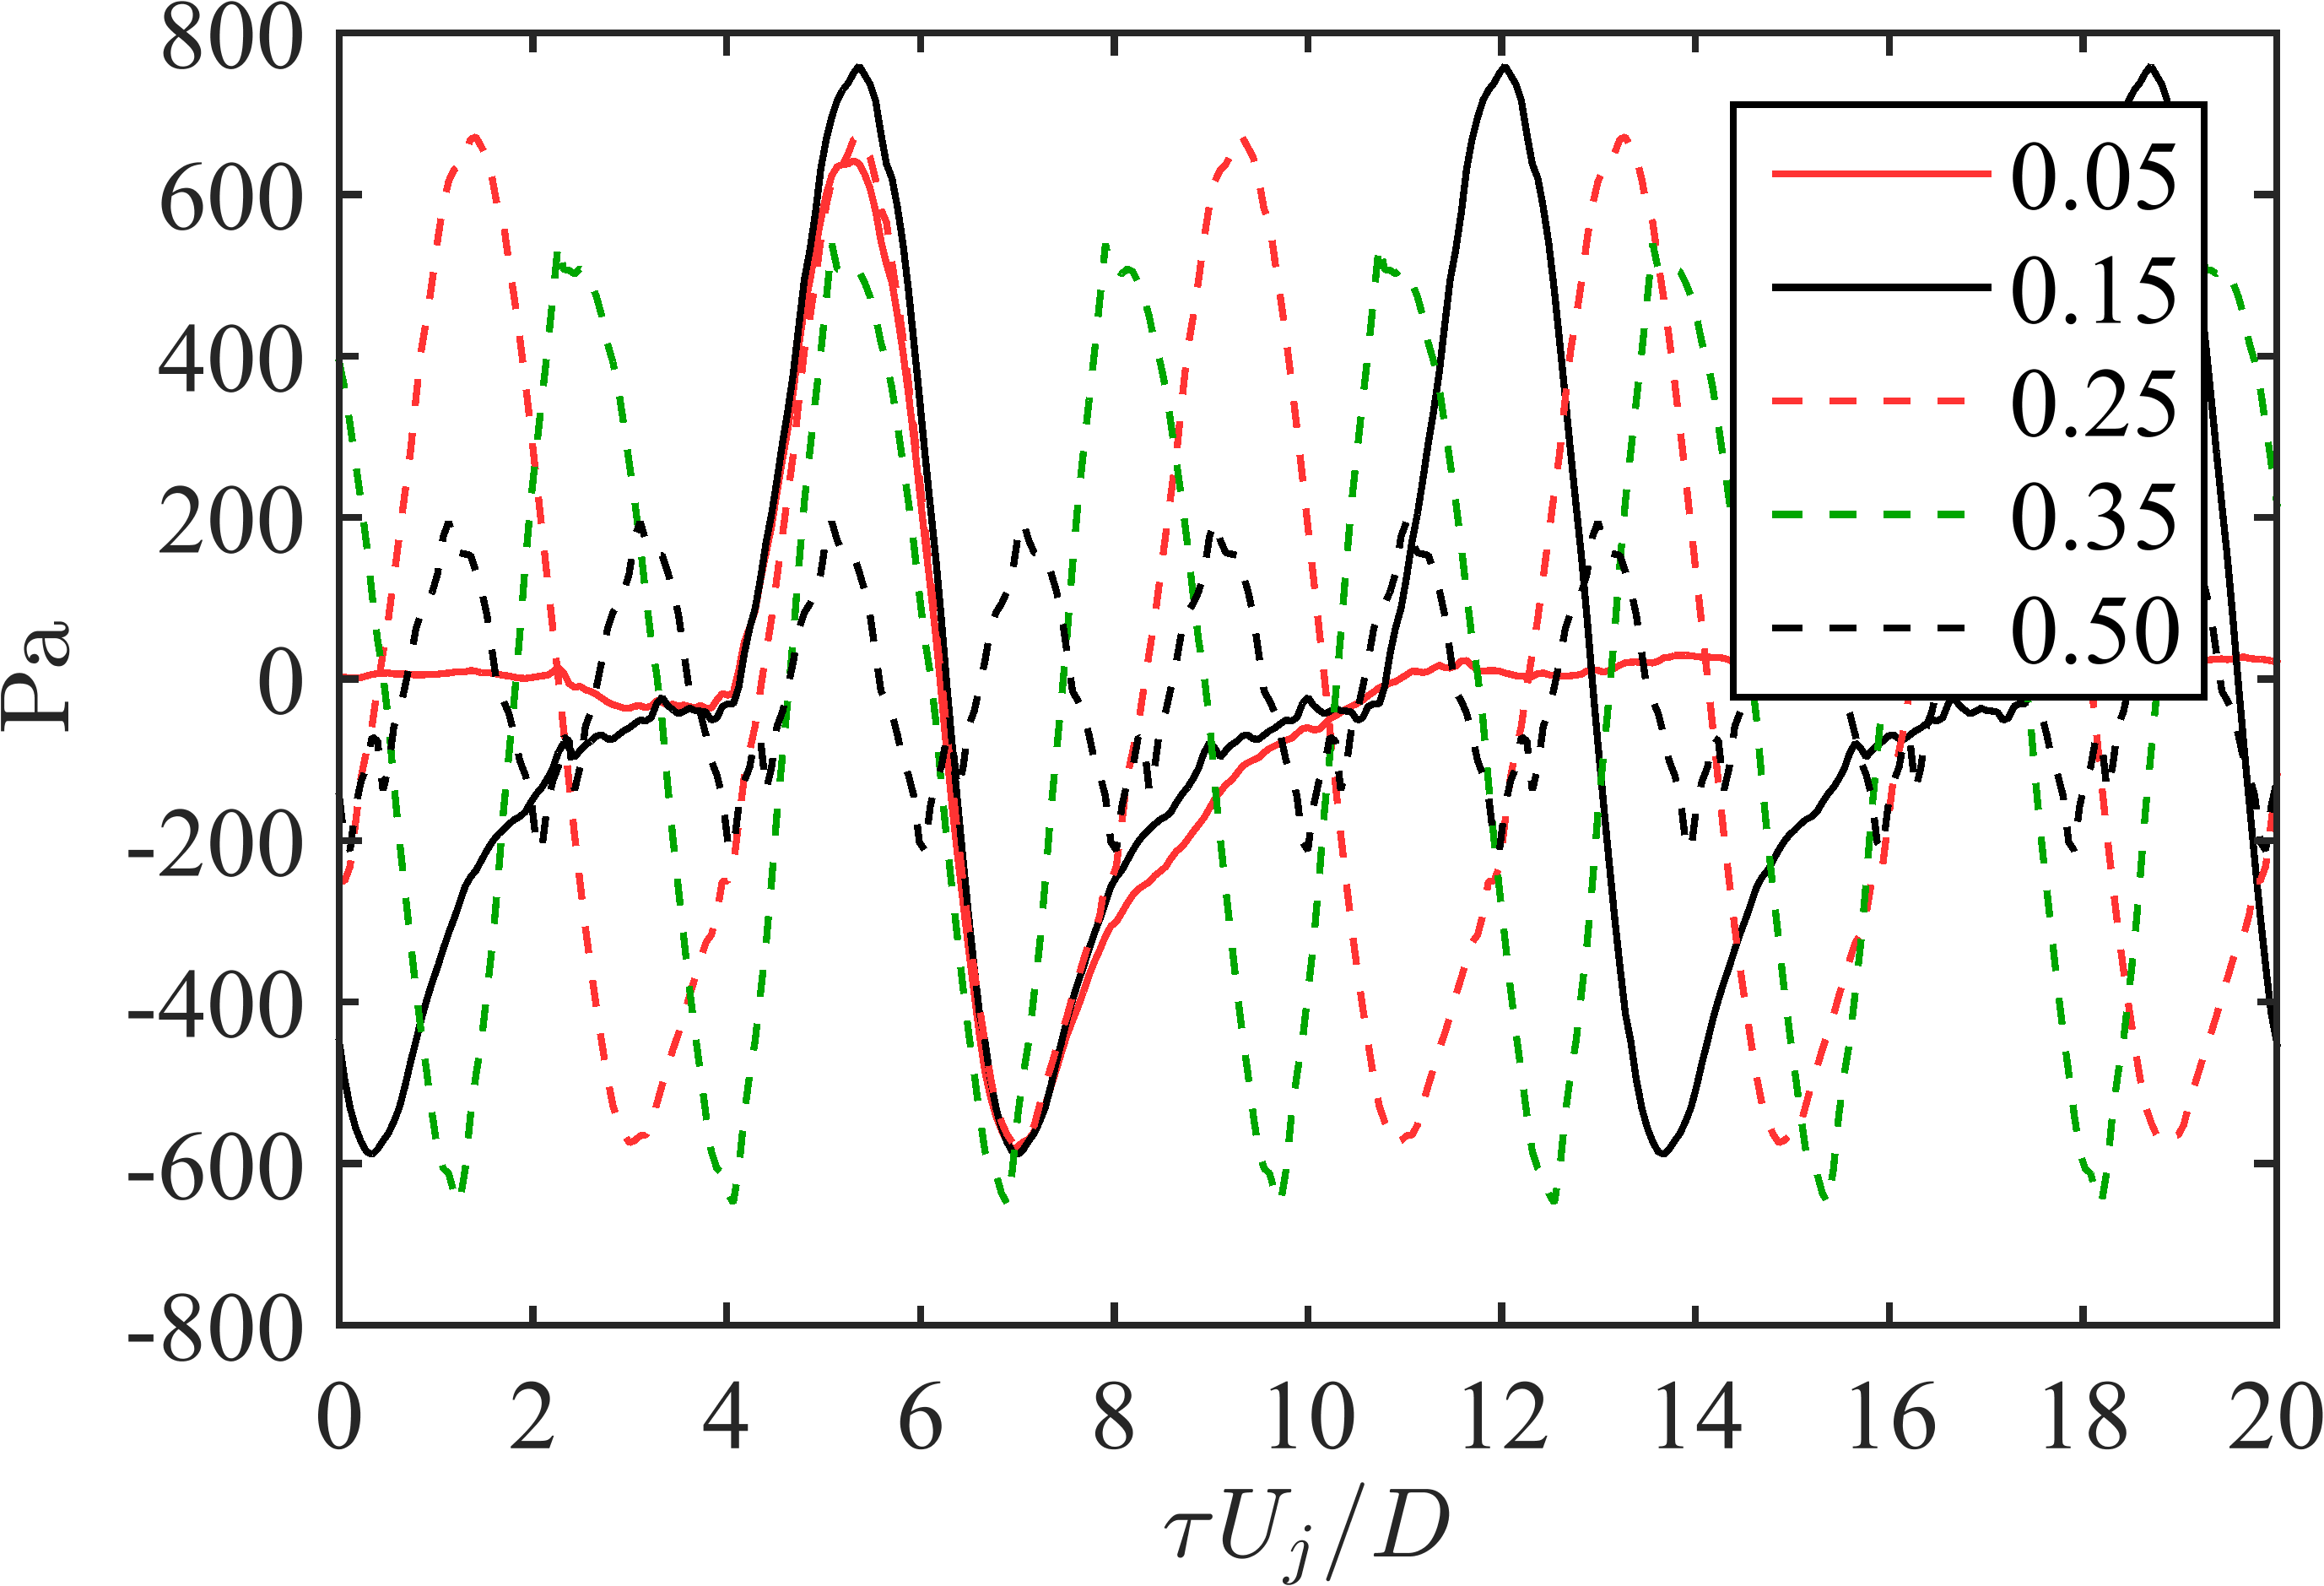
\includegraphics[width=0.95\linewidth]{Figures/ch3_nearfield_phavg_v2.png}
		\caption{}
		\label{fig:ch3_nearfield_phavg}
	\end{subfigure}%
	\begin{subfigure}{.5\textwidth}
		\centering
		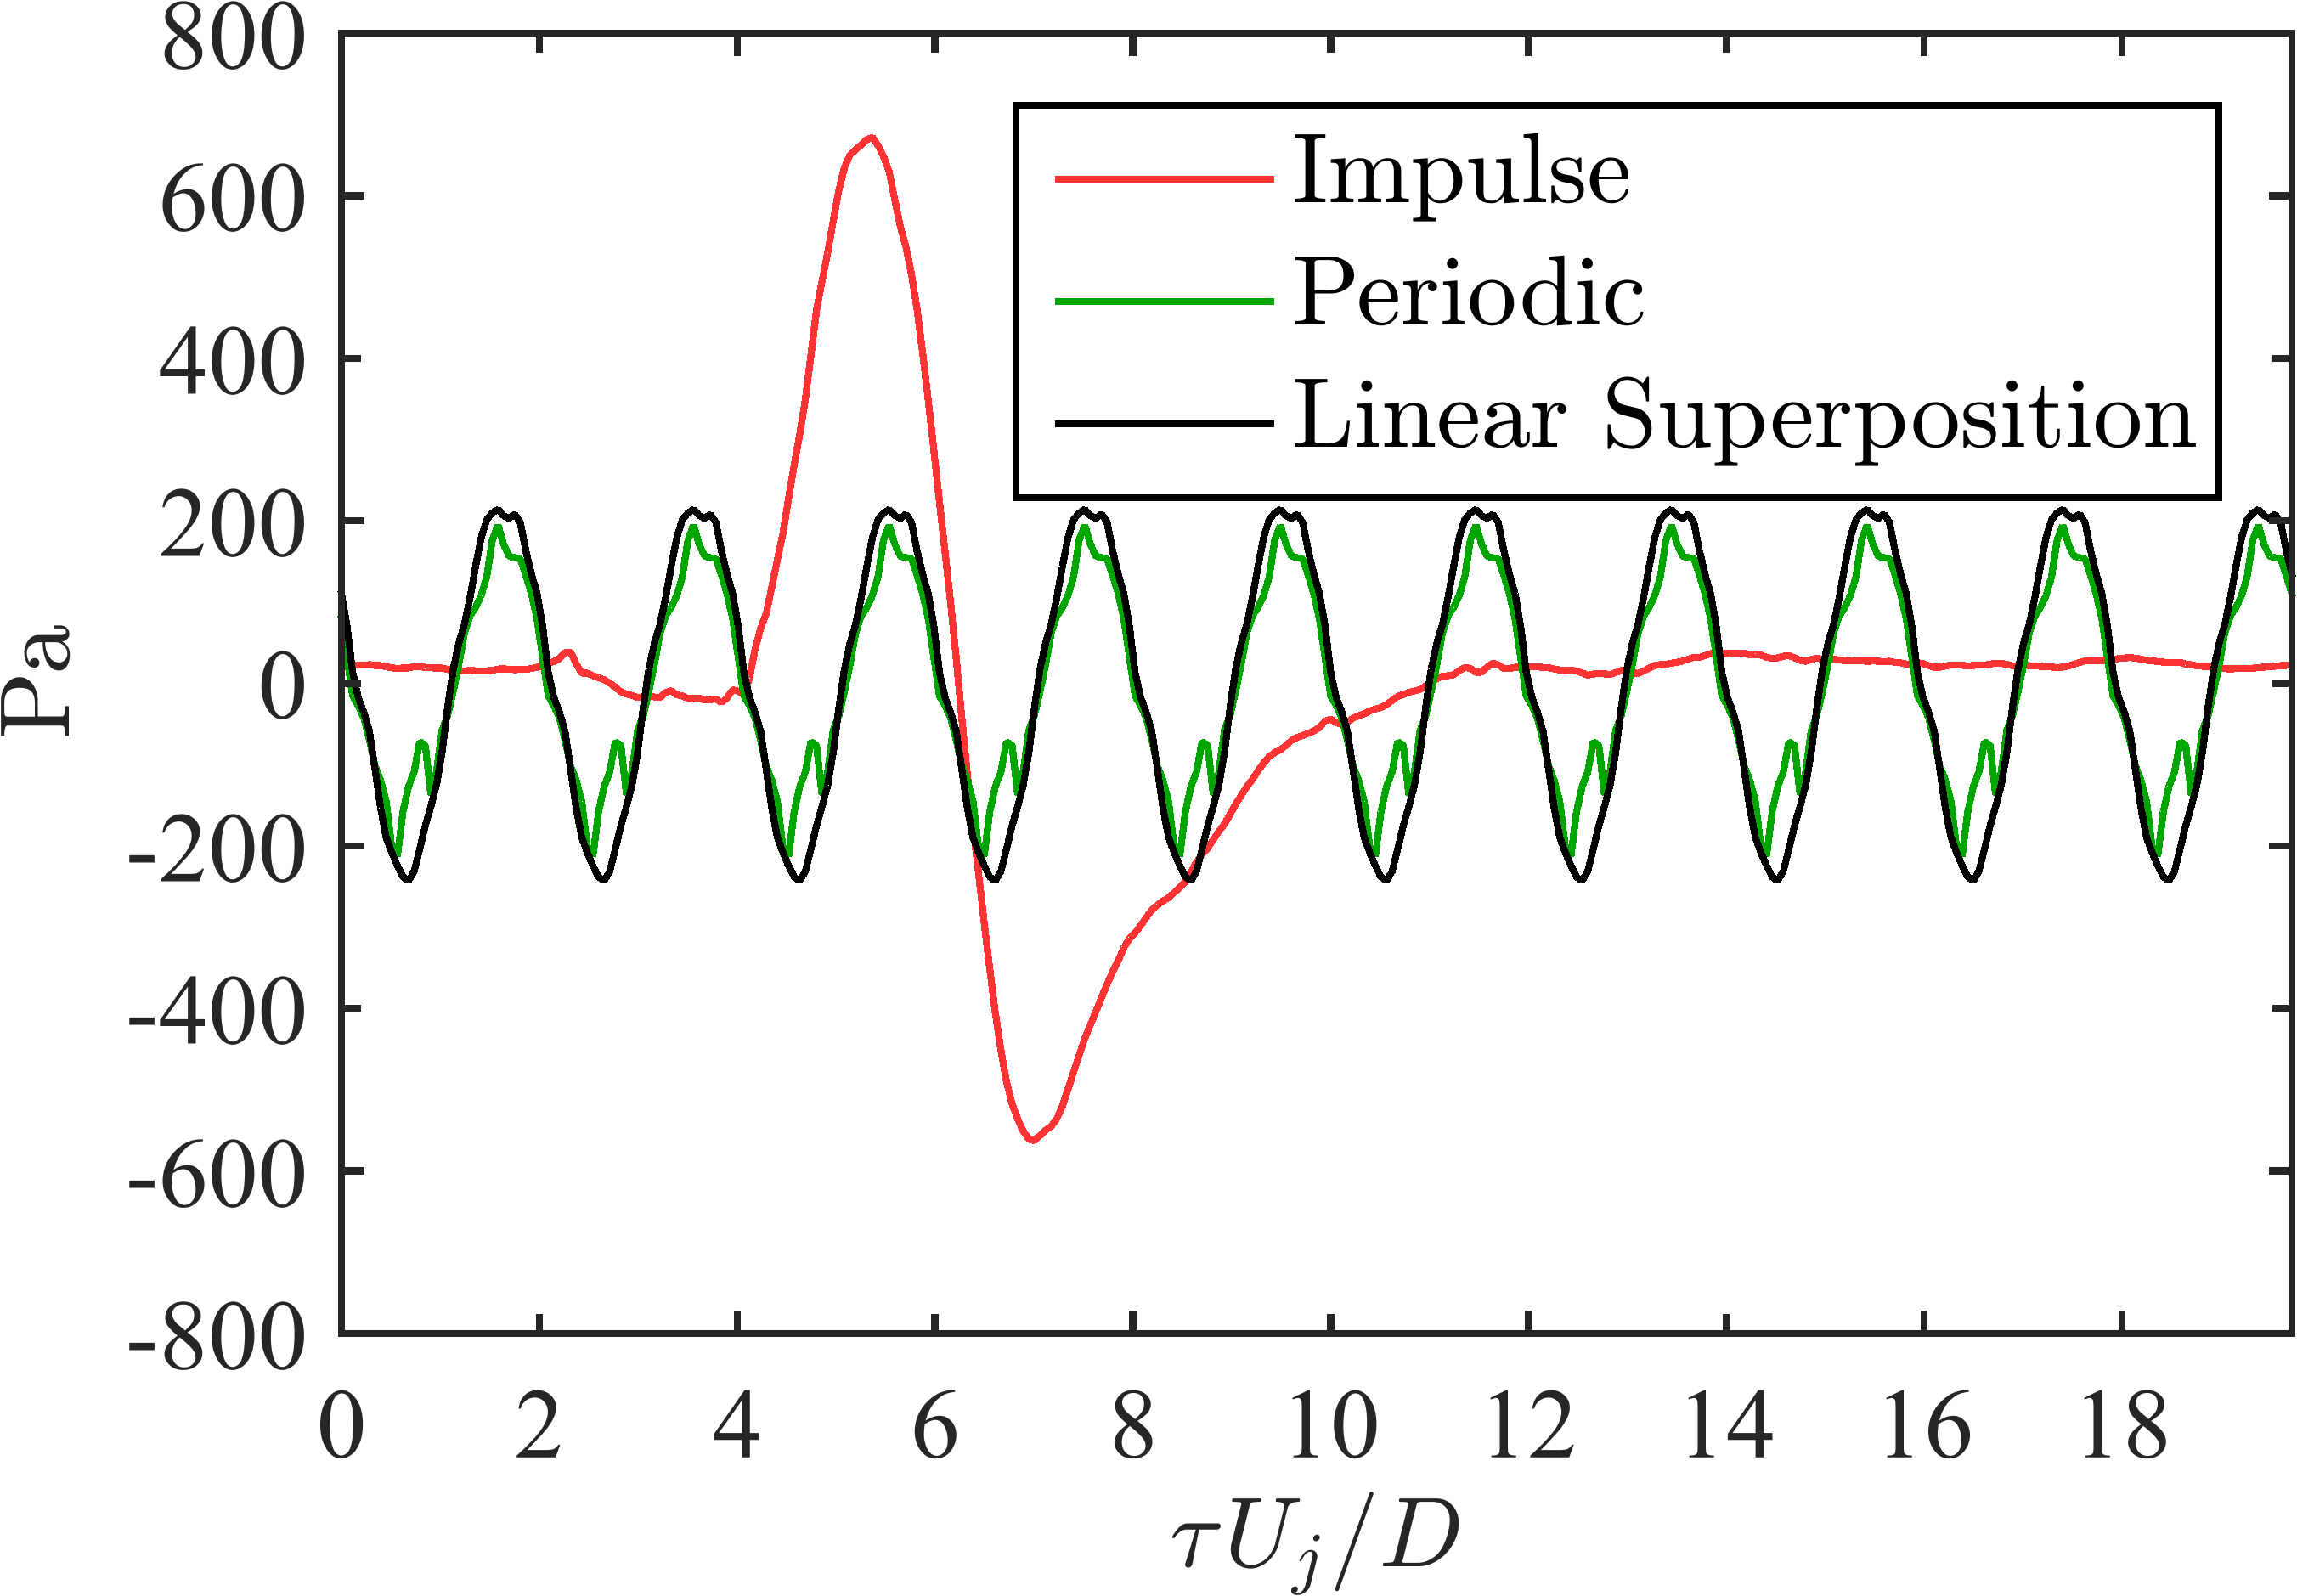
\includegraphics[width=0.95\linewidth]{Figures/ch3_nearfield_linear_v2.png}
		\caption{}
		\label{fig:ch3_nearfield_linear}
	\end{subfigure}
	\caption{Phase-averaged waveforms along the first array position at $x/D = 3, r/D = 1.35$ (a) and a linear superposition of the phase-averaged waveform for the impulse excitation ($St_{DF} = 0.05$) compared against periodic excitation ($St_{DF} = 0.50$) (b).}
	\label{fig:ch3_nearfield}
\end{figure}

For a certain range of excitation frequencies ($St_{DF} \leq 0.50$ at $x/D = 2$, for example), the structures interact in a quasi-linear manner, insofar as their near-field pressure signatures are concerned. 
To be precise, the response of the jet in the irrotational near-field could be well-predicted by a linear summation of the impulse response of the jet, repeated at the periodic excitation frequency. 
This concept has been illustrated in \fig{fig:ch3_nearfield_linear}, where the periodic response of the jet to excitation with $St_{DF} = 0.50$ has been reproduced at $x/D = 3$. 
Additionally, a linear superposition of the impulse response for $St_{DF} = 0.05$, repeated to match the excitation frequency of $St_{DF} = 0.50$, has been overlaid. 
The linear superposition has been arbitrarily shifted in time in order to match the phase of the periodic response; this phase difference is likely due to the dependence of convection velocities on structure frequency \citep{Veltin2011} (or more accurately, structure size). 
For reference, the impulse response has also been included in the plots. 
Upstream of the end of the potential core ($x/D \simeq 6$, as will be found in \sect{sect:velocity}), the quasi-linear interaction model produces close predictions of the waveform amplitude and shape, despite the significant difference in both peak amplitude and waveform shape between the impulse and periodic responses. 

This quasi-linear interaction of the jet response to excitation is not limited exclusively to the hydrodynamically-dominated regions of the jet, but in fact holds for the acoustic far-field as well, at aft angles (where the acoustic signal is strongest and is known to correlate well with large-scale structures). 
This can be observed in \fig{fig:ch3_farfield_phavg}, where the phase-averaged response of the jet has been plotted for the far-field signal at a polar angle of $30^\circ$. 
For legibility, only a select number of excitation Strouhal numbers have been included. 
As with the irrotational near field, the acoustic far field exhibits a compact waveform for the lowest excitation Strouhal numbers. 
Though nearly a direct inverse from the waveform observed in the hydrodynamically-dominated near field, the far-field waveform is quite reminiscent of the phase-averaged waveforms observed by Kambe \& Minota \citep{Kambe1983} for the acoustic radiation towards aft angles produced by the head-on collision of vortex rings. 
At higher $St_{DF}$, a continuous oscillation between sharp expansion and compression waves is again observed, though the amplitude begins to decay above moderate excitation Strouhal numbers. 
\begin{figure}
	\centering
	\begin{subfigure}{.5\textwidth}
		\centering
		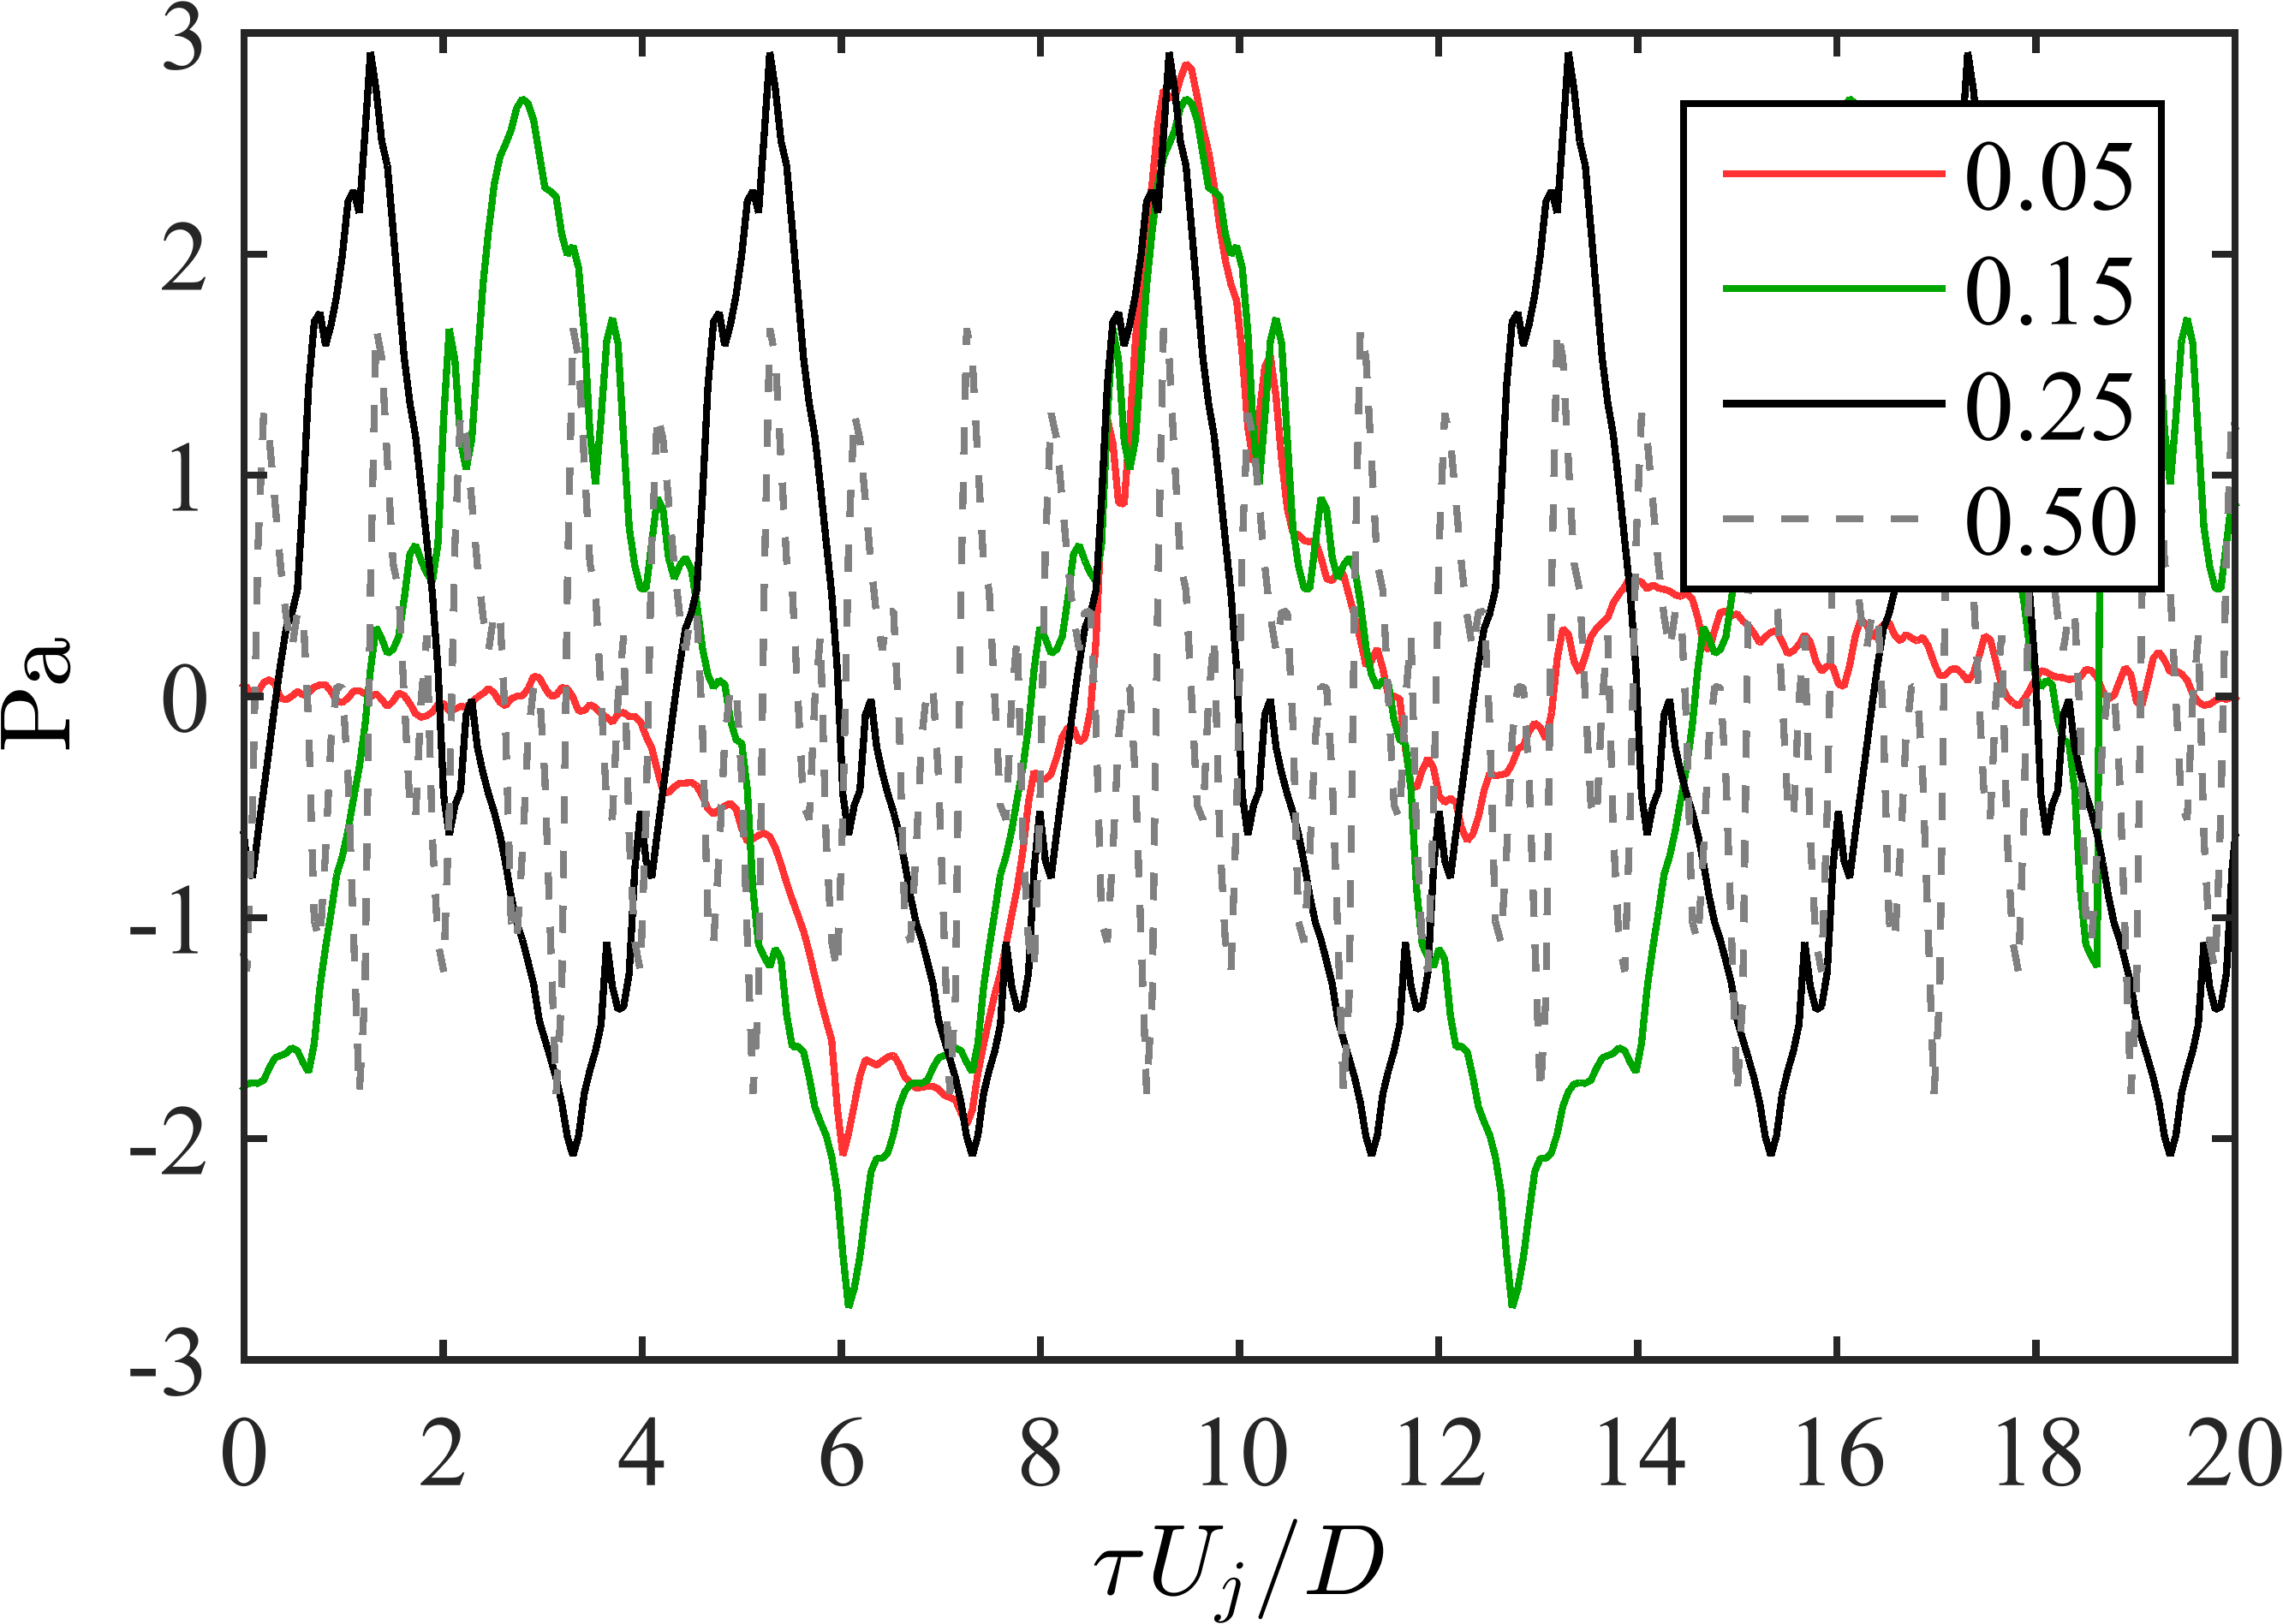
\includegraphics[width=0.95\linewidth]{Figures/ch3_farfield_phavg_v2.png}
		\caption{}
		\label{fig:ch3_farfield_phavg}
	\end{subfigure}%
	\begin{subfigure}{.5\textwidth}
		\centering
		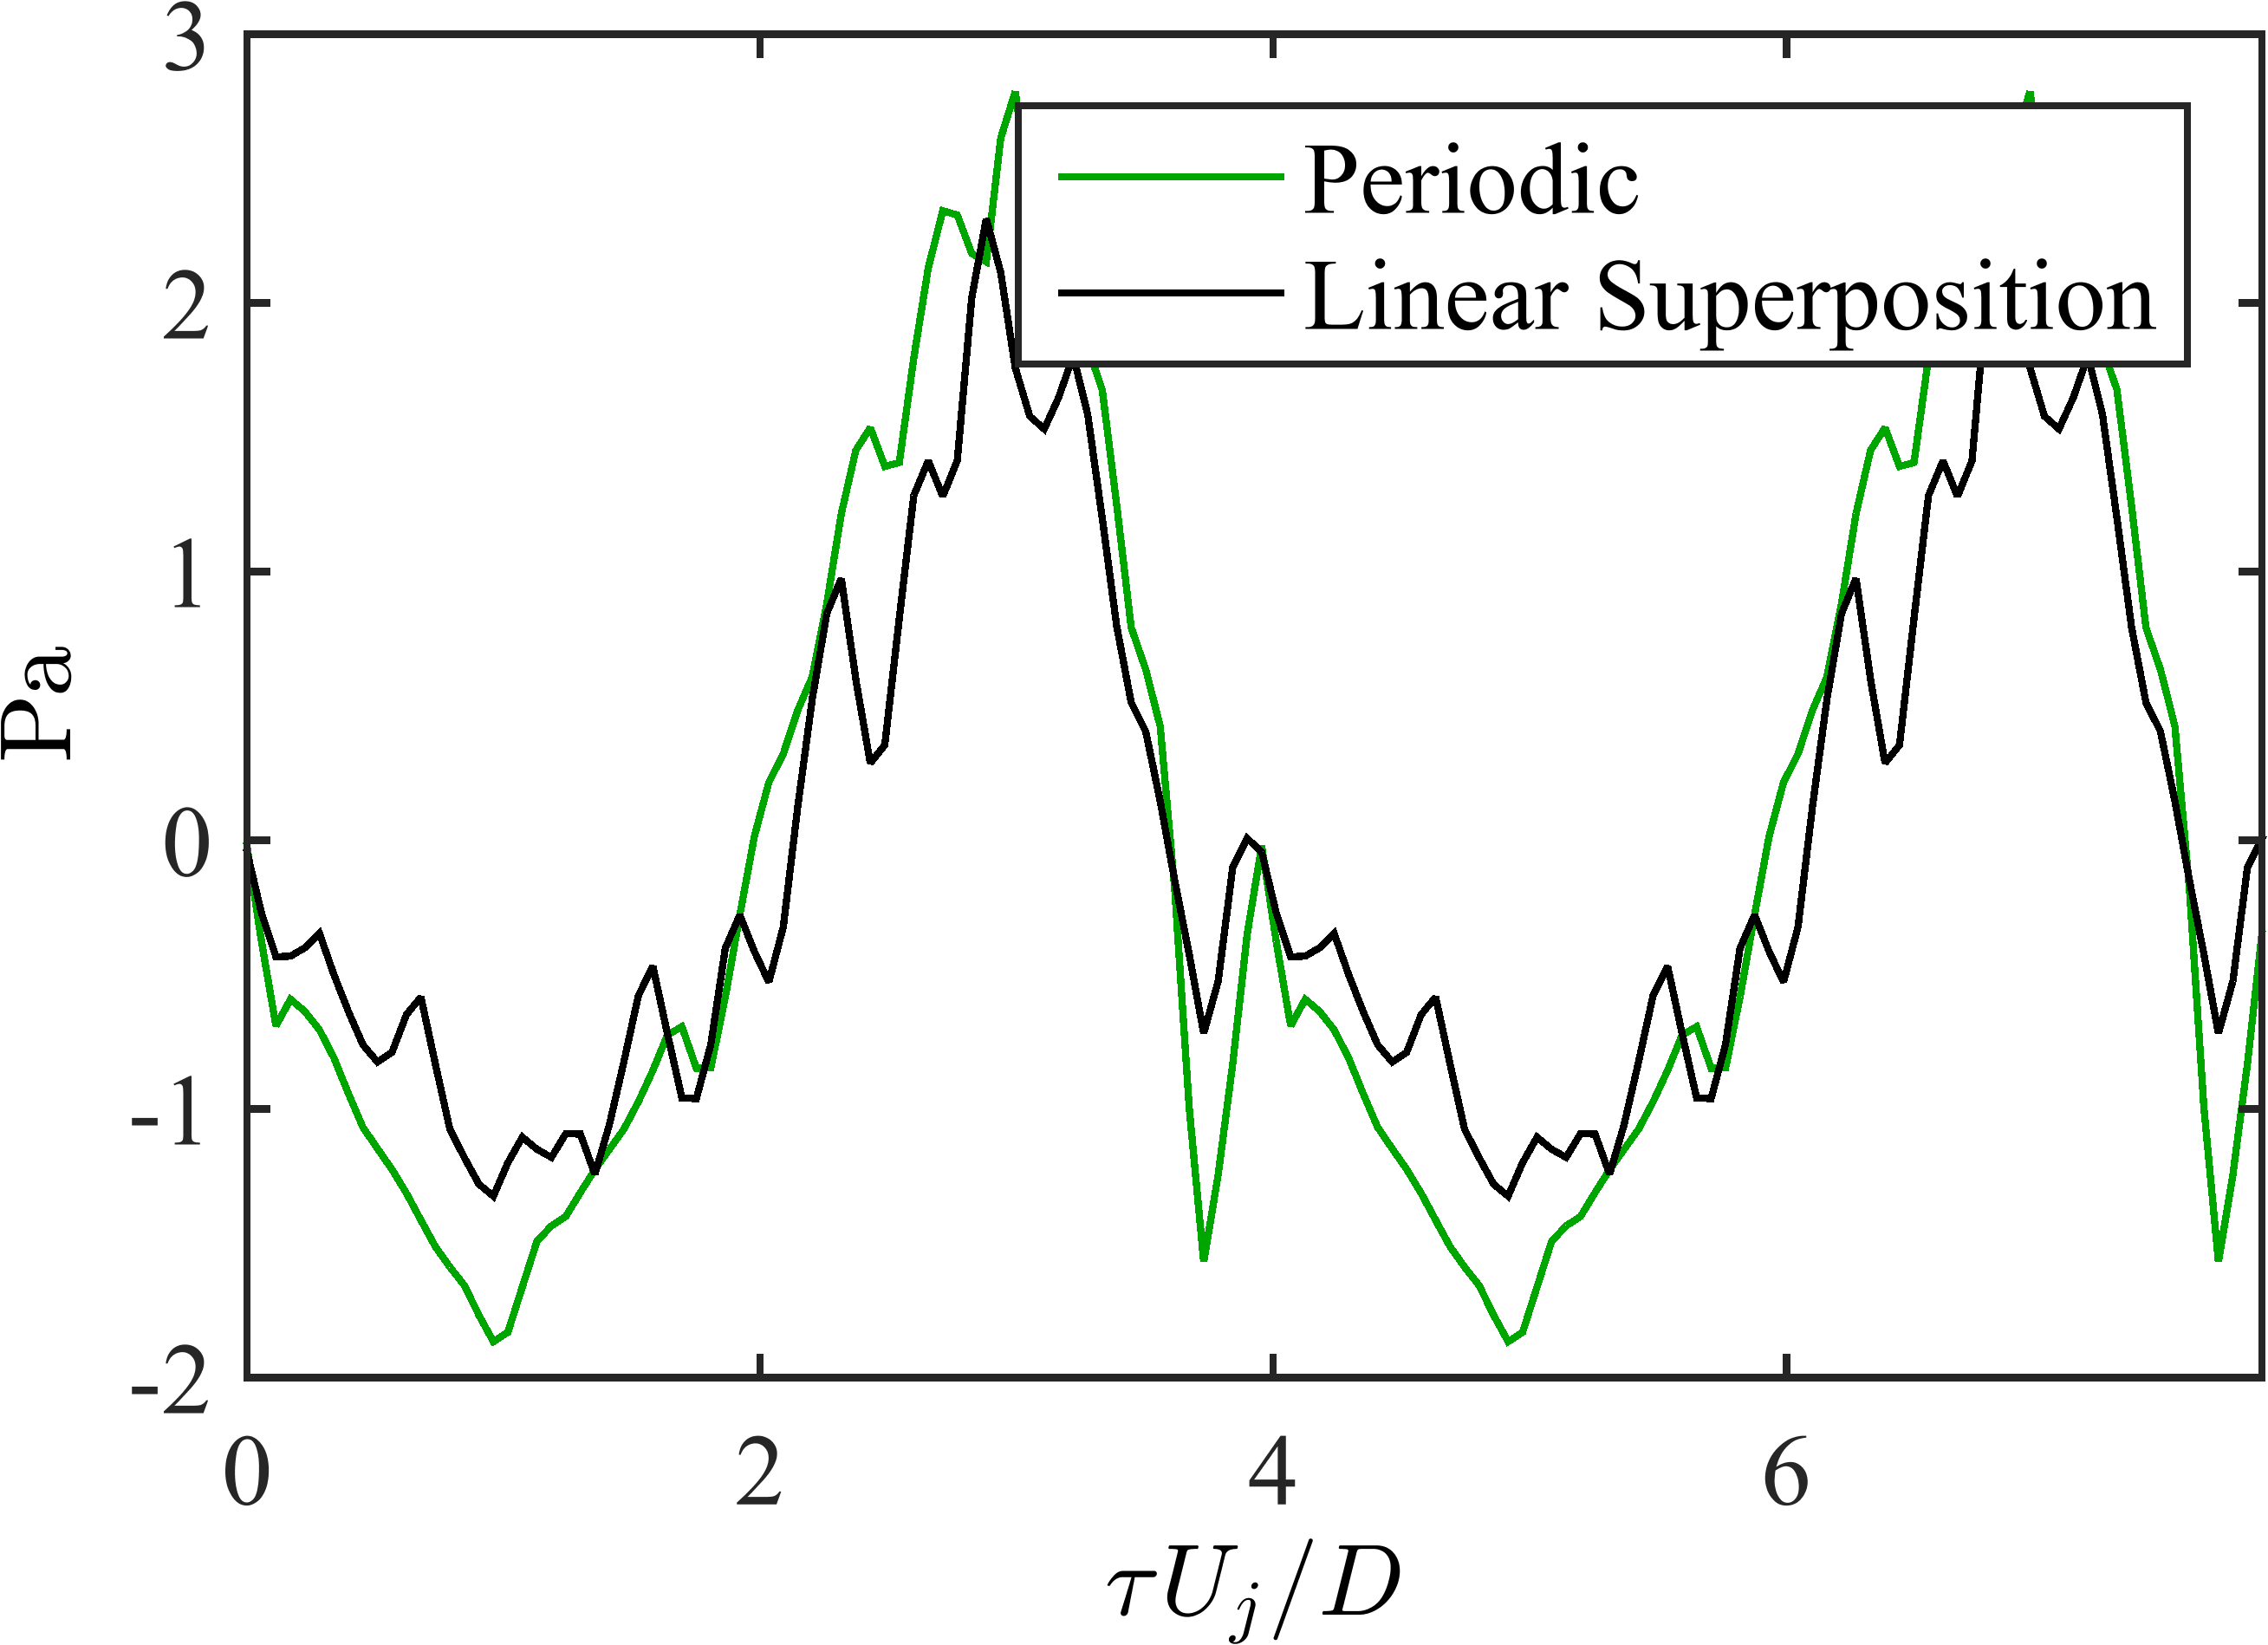
\includegraphics[width=0.95\linewidth]{Figures/ch3_farfield_linear_v2.png}
		\caption{}
		\label{fig:ch3_farfield_linear}
	\end{subfigure}
	\caption{Phase-averaged waveforms of the far-field at $30^\circ$ (a) and a linear superposition of the phase-averaged waveform for the impulse excitation ($St_{DF} = 0.05$) compared against periodic excitation ($St_{DF} = 0.25$) (b).}
	\label{fig:ch3_farfield}
\end{figure}

As before, a linear superposition of the impulse response can well predict the waveform shape and amplitude at the higher excitation frequencies (\fig{fig:ch3_farfield_linear}), though in this case only up to $St_{DF}  = 0.25$. 
From the phase-averaged waveforms alone it is not clear whether this breakdown in the linear superposition model at the highest excitation frequencies is due to nonlinear behavior or uncertainty in the phase-averaging. 
Results comparing the linear superposition of the impulse response against the measured periodic response at $St_{DF}  = 0.35$ are shown in \fig{fig:ch3_farfield_nonlinear}.
Some similarities may be found in the waveform shape and amplitude, but overall it is clear that the acoustic response of the jet to excitation at $St_{DF}  = 0.35$ is substantially modified from the response at lower frequencies.
Though this is hardly conclusive in its own right, this result does suggest either changing or competing acoustic source mechanisms are present in these excited jets.
The phase-averaged waveforms were also investigated at polar angles of $60^\circ$ and $90^\circ$; however a clear waveform was not identifiable over the statistical uncertainty inherent in the phase-averaging process (likely due to the superdirective character of the acoustic radiation \citep{Crighton1990}, which renders the amplitude at sideline angles too low to be detectable).
Additional details and analysis of the phase-averaged near- and far-field signals can be found in Crawley \etal \citep{Crawley2015}.
\begin{figure}
	\centering
	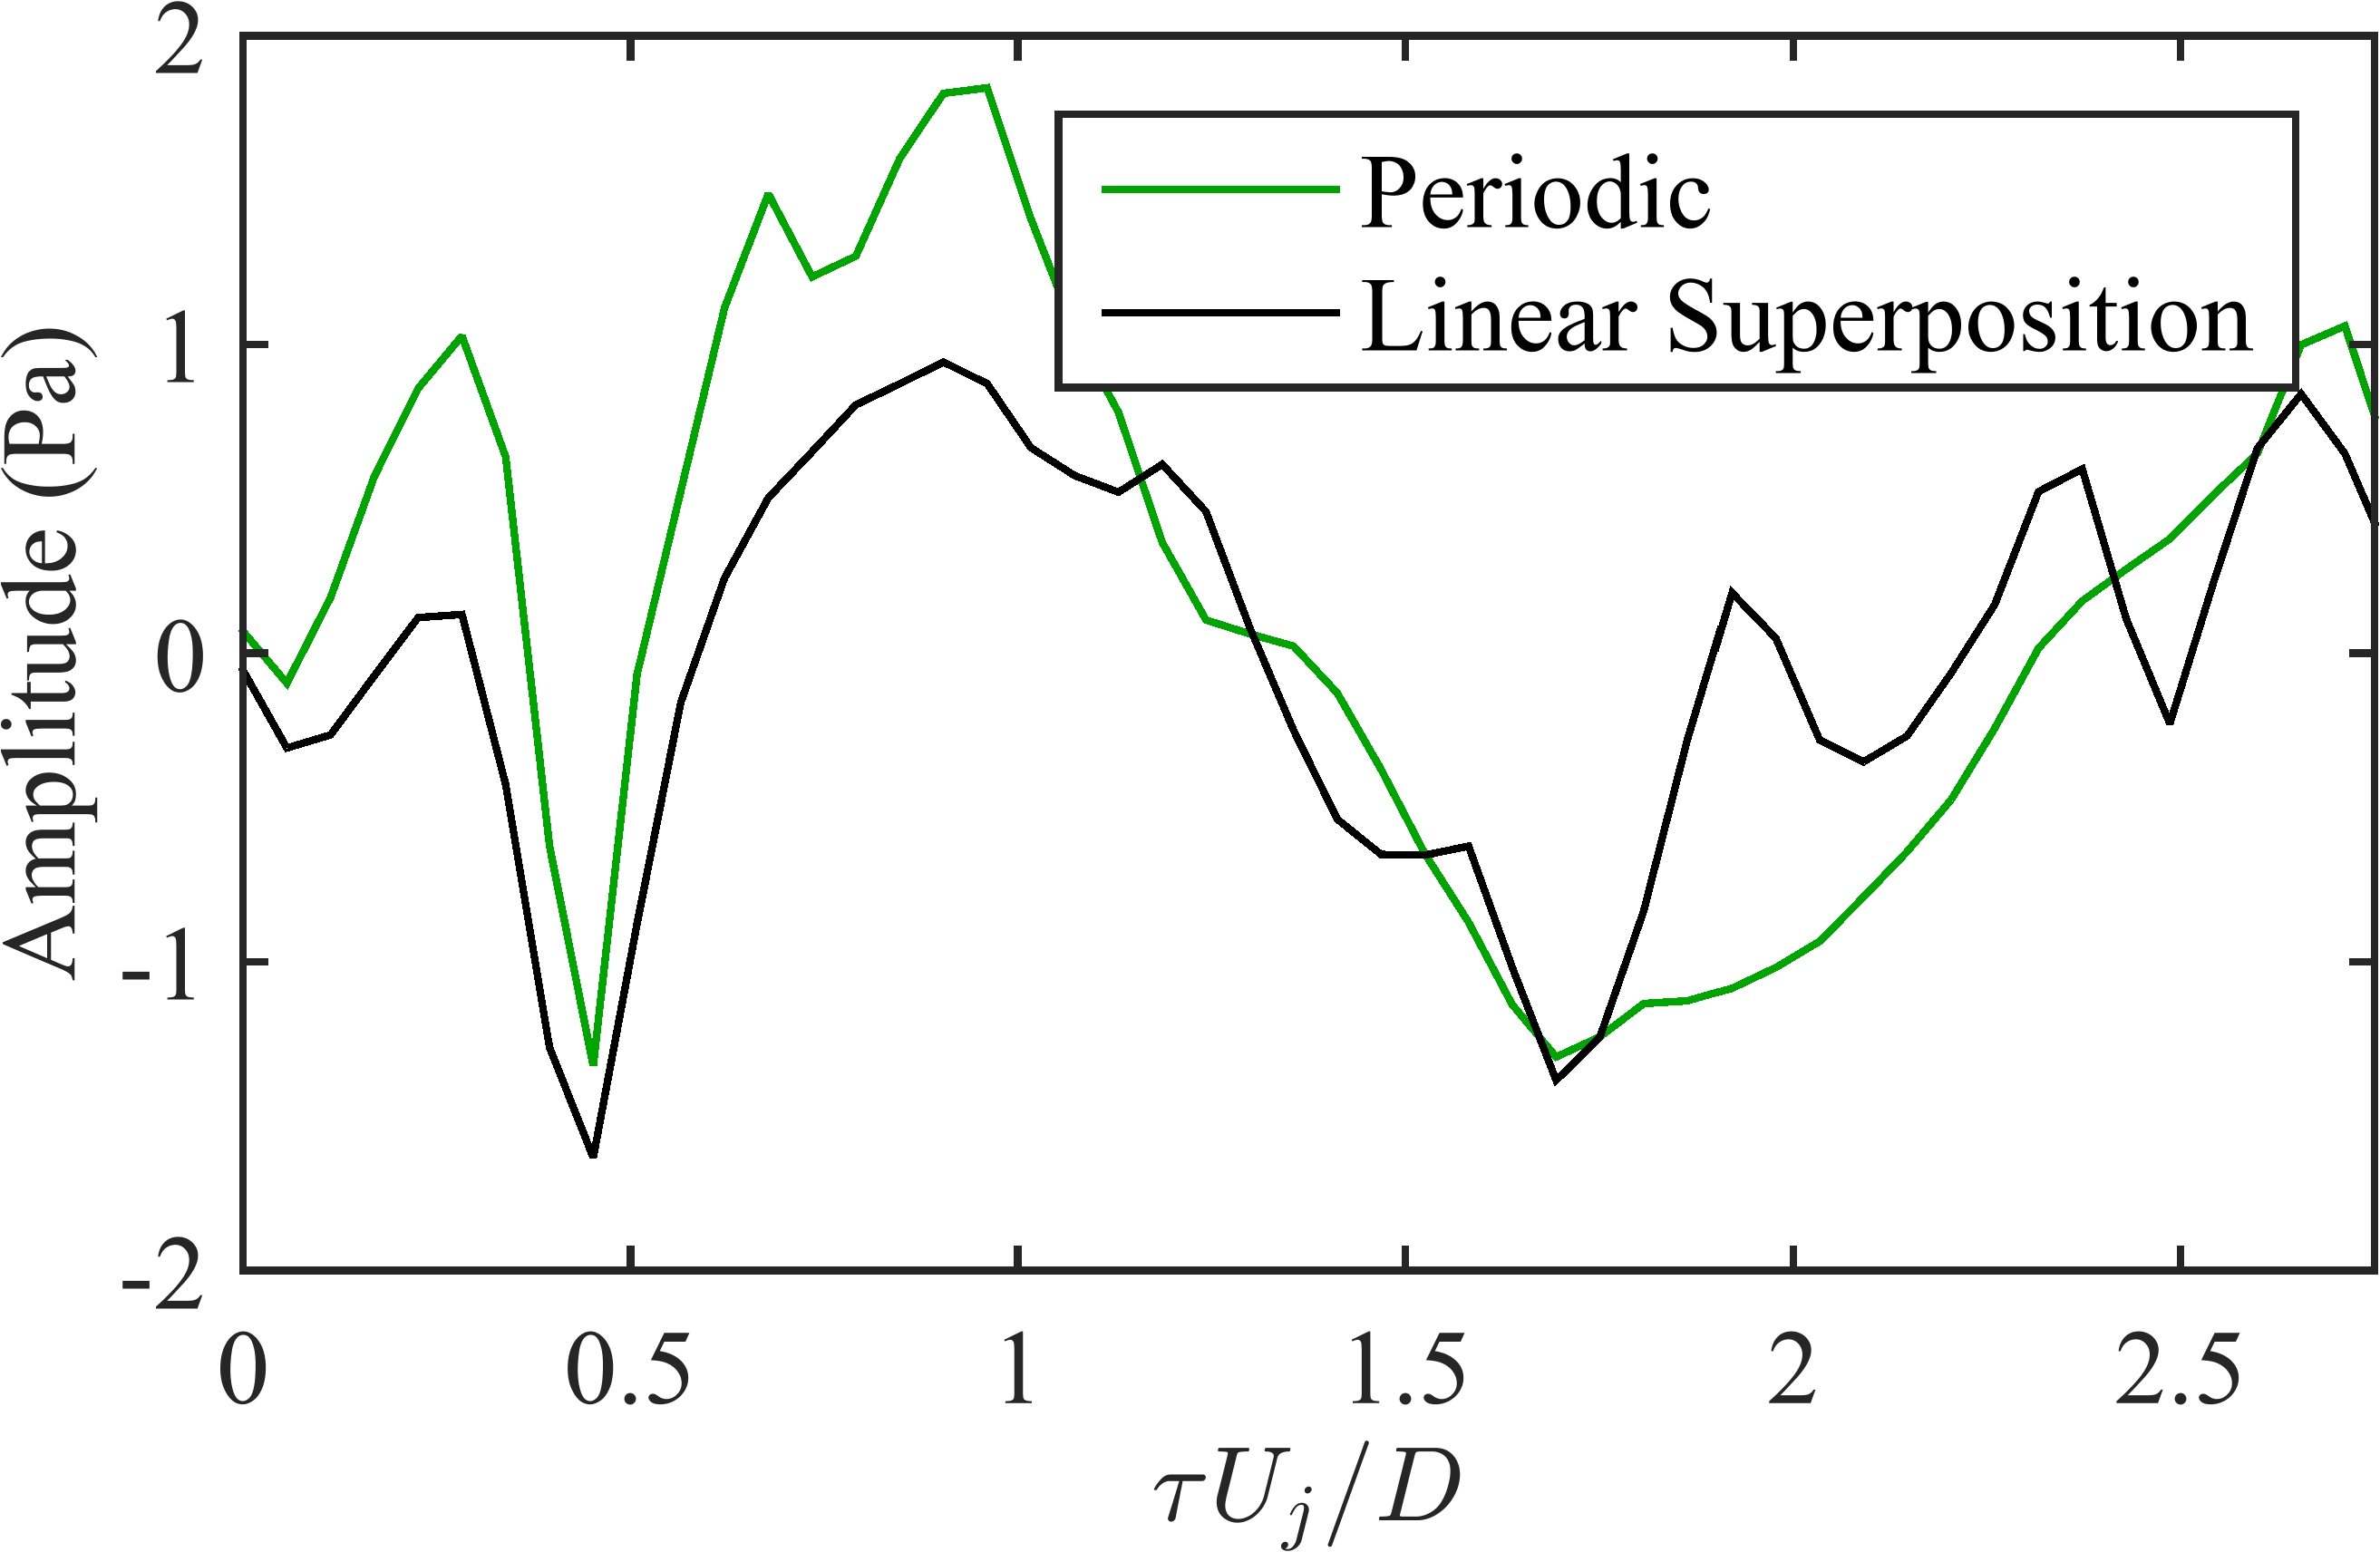
\includegraphics[width=3.5in]{Figures/ch3_farfield_linearsuperposition_st035_v2.png}
	\caption{Linear superposition of the phase-averaged impulse response to excitation against the measured periodic response for $St_{DF} = 0.25$ at the  $30^\circ$ far-field microphone.}
	\label{fig:ch3_farfield_nonlinear}
\end{figure}

\section{Preprocessing: Filtering the Actuator Self-Noise}
Analysis of the near-field response of the forced jet is not immediately straightforward due to acoustic contamination from the actuators themselves \citep{Sinha2012}. 
LAFPAs operate on a joule heating principle: the breakdown of the air between the electrodes and the ensuing flow of current results in intense heating of the air. This rapid, localized thermal perturbation produces a compression wave, which excites the shear layer. 
However, this compression wave is still evident as it travels through the near field. 
Multiple compression waves can clearly be seen in \fig{fig:self-noise}, in which a subsonic rectangular jet is being excited at 20 kHz by four LAFPAs on its lower edge. \begin{figure}
	\centering
	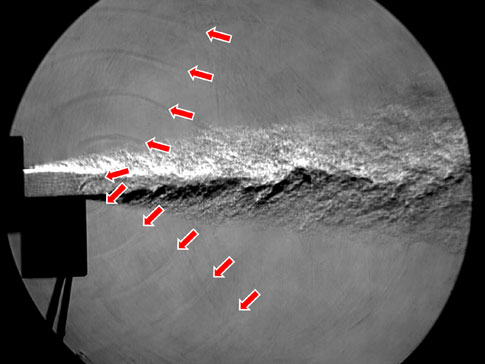
\includegraphics{Figures/Samimy2010JFM.jpg}
	\caption{Schlieren image highlighting LAFPA compression waves. Reprinted from Samimy \etal \cite{Samimy2010}.}
	\label{fig:self-noise}
\end{figure}

Obviously, this is an undesirable effect, as this actuator self-noise may in some cases obscure the hydrodynamic and acoustic response of the jet.
So, in the present work the near-field pressure signals have been preprocessed using a continuous-wavelet-based filtering algorithm, which has been specifically designed to remove the actuator self-noise while leaving the signature of the jet response unaltered. 
An example of this filtering can be found in \fig{fig:preprocessing:wavelet_filter}, where the raw and preprocessed signals have been plotted for $St_{DF} = 0.02$ at $x/D = 1$, $r/D = 1.20$. 
To aid in visualization, the results for multiple excitation periods has been phase-averaged to produce these waveforms. 
As the actuator self-noise is localized in both time and frequency and can be well predicted, a smoothing algorithm in the wavelet domain was found to be the most effective method for removing the undesirable noise while leaving the response of the jet intact. 
A fourth-order Paul wavelet is employed, due to the similarity of its imaginary component to the phase-averaged response of the jet. 
As a result, the energy of the response of the jet is well defined in the wavelet domain, with the actuator self-noise existing as high-frequency, temporally-localized oscillations superimposed on the field. 
After smoothing in the wavelet domain to remove these oscillations, the signal is transformed back into the physical domain where it undergoes another smoothing operation in order to remove small amplitude, high frequency oscillations which may be introduced by the wavelet-smoothing. 
For consistency hereafter, all results examined within this work have been computed from the filtered, rather than the raw, signals.
\begin{figure}
	\centering
	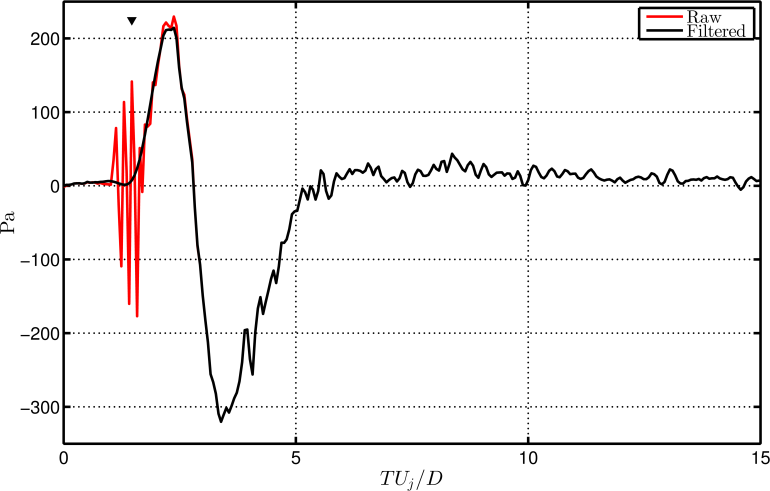
\includegraphics{Figures/NearField_Preprocessing_Filtering.png}
	\caption{Raw and preprocessed near-field pressure.}
	\label{fig:preprocessing:wavelet_filter}
\end{figure} 

\section{Acoustic/Hydrodynamic Decomposition}
\label{sect:ac_decomp}
Much of the difficulty in identifying the aeroacoustic source terms revolves around the dissimilar range of scales and fluctuation intensities of the turbulent eddies in the shear layer and the resulting radiated noise. 
Outside the jet shear layer, in the irrotational near-field of the jet, strong hydrodynamic pressure fluctuations associated directly with the passage of coherent structures in the shear layer and their resultant weak acoustic radiation coexist \citep{Arndt1997}. 
Beyond this, in the acoustic far-field, the hydrodynamic signature of the coherent structures is nonexistent owing to their strong exponential decay with radial distance.
Much work has focused in the irrotational near-field, in order to improve the aeroacoustic community's understanding of the link between shear layer turbulence and far-field acoustic radiation. 

Owing to the presence of strong hydrodynamic fluctuations dominating the irrotational pressure field near the noise source regions, identification of pure acoustic waves and their corresponding source events is problematic.
A decomposition of the pressure field into its constitutive hydrodynamic and acoustic components is therefore required. 
By identification and prediction of coherence nulls in the near field, Coiffet \etal \citep{Coiffet2006} showed that the full irrotational near-field consistent primarily as a linear superposition of its hydrodynamic and acoustic components, which lead subsequent researchers to propose linear filters to extract the individual components from the near-field pressure, with varying degrees of success. 

As discussed by Tinney \& Jordan \citep{Tinney2008}, in a transonic jet in which the large-scale structures are convecting subsonically with respect to the ambient speed of sound, a demarcation of the hydrodynamic and acoustic energy fields can be observed with phase velocity.
This is because the hydrodynamic pressure fluctuations will be aligned with the jet axis, and travelling subsonically. 
Acoustic pressure fluctuations will impinge on the linear microphone array at oblique angles, and therefore will appear as having either sonic or supersonic phase velocity, based on the source location. 
Therefore, a demarcaction between the hydrodynamic and acoustic energy components should be readily identifiable about the sonic wavenumber, $k_a = \omega / a_\infty$.

An illustration of this can be found in \fig{fig:phase_velocity_map}, where the power spectral density of the irrotational near-field pressure for a single microphone array position has been plotted as a function of normalized frequency and (axial) wavenumber.
The sonic velocity has been identified with a dashed line; energies lying above this line correspond to supersonically traveling waves (and hence, acoustic energy) whereas energies below this line correspond to subsonically convecting waves (hydrodynamic energy).
Note that at high wavenumber and frequencies, two distinct energy lobes become readily apparent.

This phase-velocity separation is the basis for the decomposition method of Tinney \& Jordan \citep{Tinney2008}, which used a Fourier-based wavenumber-frequency filter in a cold, subsonic jet to separate the near-field pressure into supersonically- and subsonically-convecting waves.
The pressure field is first transformed into Fourier space ($k_x,\omega$), as
\begin{equation}
	\hat{p} \left( k_x , \omega \right) = \iint_{\mathbb{R}^2} p(x,t)e^{-i(\omega t - k_x x)}dxdt
\end{equation}
From the transformed pressure field, the hydrodynamic and acoustic fields can then be reconstructed separately, from
\begin{equation}
	p_c (x,t) = \frac{1}{(2 \pi)^2} \iint_{\mathbb{R}^2} \phi_c (k_x,\omega) \hat{p} (k_x,\omega)e^{i(\omega t - k_x x)}dk_x d\omega .
	\label{eq:fourier_filter}
\end{equation}
The component weight vector, $\phi_c \in [0,1]$, is set based on the measured axial phase velocity, $c = \omega / k_x$, in order to filter out either the supersonic or subsonic portion of the spectra. 
 
Grizzi \& Camussi \citep{Grizzi2012} took a slightly different approach, which utilized a discrete wavelet transform at individual spatial locations in order to decompose the fields based on an energy cutoff. 
The energy threshold was set iteratively, using analysis of two-point correlations of the acoustic and hydrodynamic components between two microphones, in order to ensure that realistic phase-velocities for the components were met. 
The Empirical Mode Decomposition (EMD) based method of Kuo \etal \citep{Kuo2013} dispensed with explicit concerns with the phase velocity of the pressure components and instead used the critical frequency, as defined by Arndt \etal \citep{Arndt1997}, which demarcates the energy dominance of the acoustic and hydrodynamic components in the near-field spectra.
\begin{figure}
	\centering
	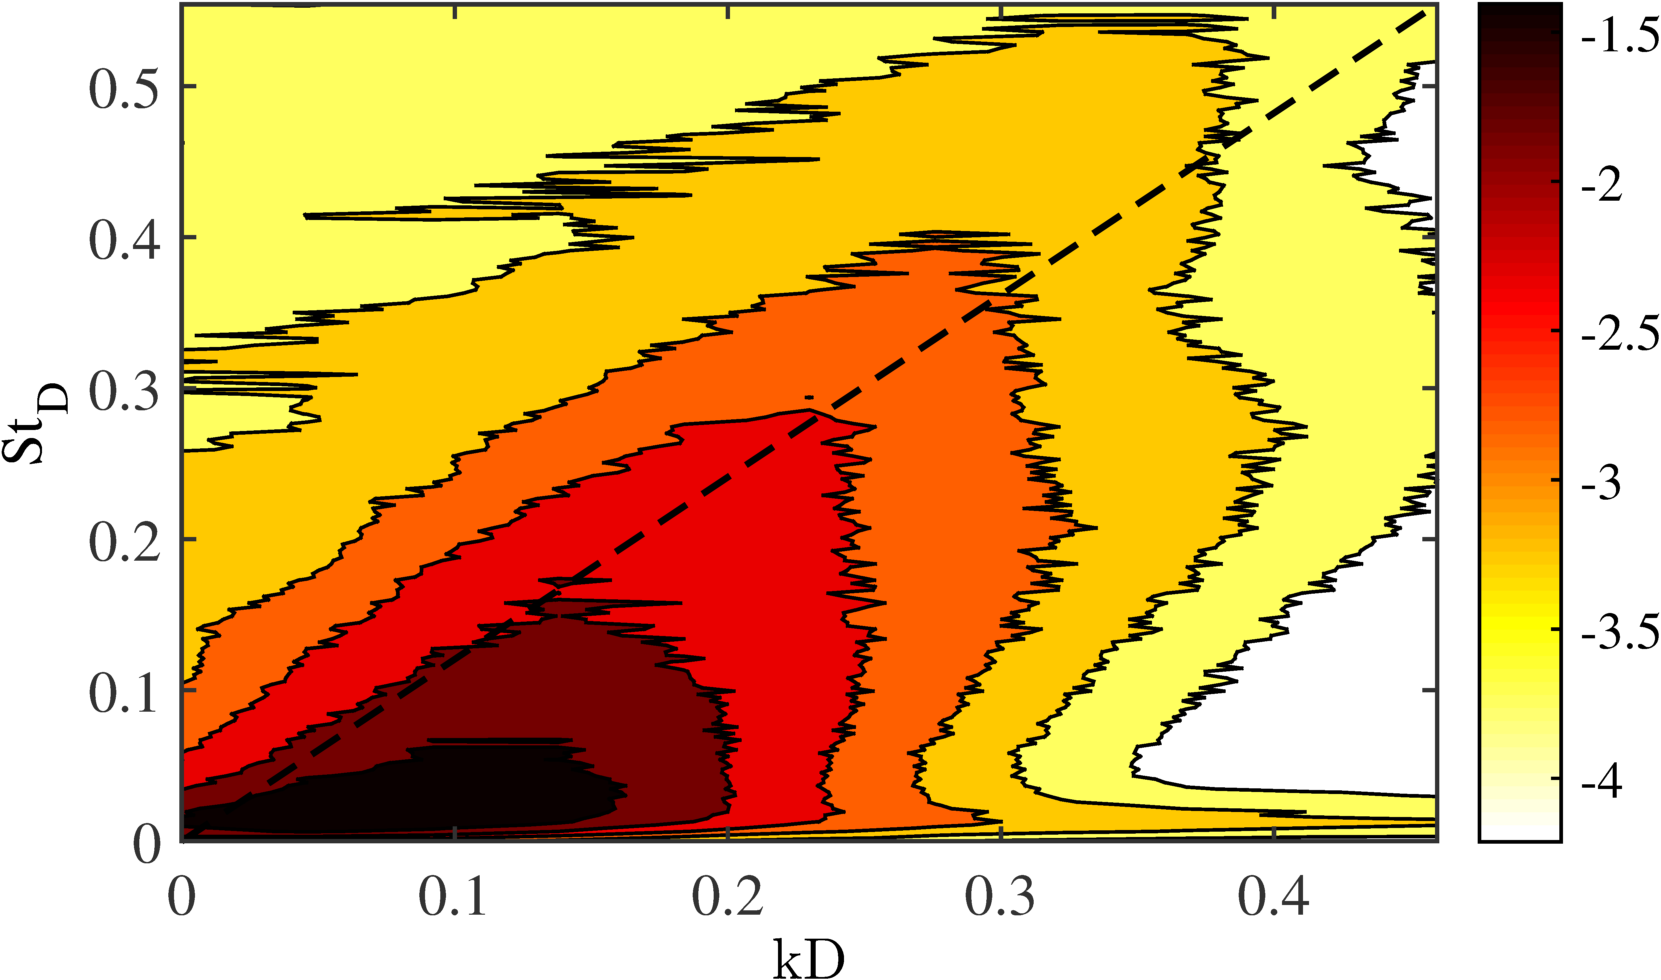
\includegraphics[width=4in]{Figures/Phase_Velocity_Map.png}
	\caption{Wavenumber-Frequency spectral energy.}
	\label{fig:phase_velocity_map}
\end{figure}

In the current work, the irrotational near-field pressure is decomposed into its constitutive hydrodynamic and acoustic components based on phase-velocity. 
The current method is similar to that of Tinney \& Jordan \citep{Tinney2008} in that an axial array of many microphones is used, though it differs in how it identifies components of different phase-velocity.
Here, the filtering will be performed by a spatio-temporal continuous wavelet transform.

\subsection{The Wavelet Transform}
Fourier analysis is commonly employed in the aeroacoustics community to study fundamental aspects of jet noise due to its simplicity and the great abundance of information it can provide. 
However, there is also a great drawback associated with Fourier analysis: while it analyzes a given signal at a distinct frequency, local information for a given event is spread over all spectral coefficients. 
This is due to the fact that the basis functions used by the Fourier transform oscillate indefinitely. 
For a signal composed of completely random fluctuations this is not an issue, however it has become increasingly clear that the jet noise phenomenon is not a random process \citep{Kearney-Fischer2013}.
Transient events, such as intermittency or the spatial and temporal modulation of a wavepacket, have been shown to be important in the noise generation process. 

Morlet \citep{Morlet1981} introduced the wavelet transform in an effort to overcome some of the shortcomings of the Fourier transform.
Unlike the Fourier transform, the wavelet transform involves a convolution of the signal with a set of basis functions which decay to zero at the bounds.
As a direct result, translation of the basis function in space and/or time is now meaningful. 
The basis functions (often referred to as the analyzing or daughter wavelets) are all derived from a single function, the mother wavelet, which must satisfy certain criteria \citep{Farge1992},
Most notable of these criteria is that of admissibility, which in essence requires that the wavelet must be of finite energy. 
In practice, it is also helpful to choose a mother wavelet which is well-localized in both the spatio-temporal domain and the frequency domain. 
For a given mother wavelet, $\psi (\vec{x})$, the daughter wavelets can be constructed as
\begin{equation}
	\psi_d \left( \vec{x};s,\vec{\tau},\theta \right) = s^{-n/2} \psi \left( s^{-1} r_{-\theta} \left(\vec{x}-\vec{\tau} \right) \right) \
	\label{eq:daughter_wavelets}
\end{equation}
where $s$ is the scale factor, $\vec{\tau}$ the translation parameter, and in the case of a multidimensional transform, $r_{-\theta}$ is the rotation vector (which can be neglected for an isotropic mother wavelet). 
The $s^{-n/2}$ factor ensures constant energy across all dilations. 
For a specific scale, translation, and rotation, the wavelet transform then becomes
\begin{equation}
	\tilde{f} \left( s, \vec{\tau}, \theta \right) = \int_{\mathbb{R}^n} f \left( \vec{x} \right) \psi^*_d \left( \vec{x};s,\vec{\tau},\theta \right) d^n \vec{x}.
\end{equation}

Because the basis functions of the wavelet transform are of finite energy, the locality of information in the original signal is preserved in the wavelet coefficients. 
This allows the identification, analysis, and reconstruction of localized events in the original signal, something not possible with the Fourier transform, which spreads temporal/spatial information over all transform coefficients. 
This has enabled previous researchers to perform a range of new analysis techniques to turbulence and acoustic phenomena not possible with the traditional Fourier transform. An excellent review of the development of wavelet analysis as well as applications to turbulence can be found in Farge \citep{Farge1992}.

Use of a multidimensional, continuous wavelet transform to extract intermittent events with a specific phase-velocity is not immediately straightforward, due to the global nature of the scale factor. 
A `speed-tuning' parameter, $c$, was introduced to the wavelet transform (now specifically referred to as a \textit{spatio-temporal} wavelet transform) by Antoine \etal \citep{Antoine2004}, who used it for use in motion tracking and identification in two-dimensional images. 
The definition for the daughter wavelets (\ref{eq:daughter_wavelets}) is modified to
\begin{equation}
	\psi_d \left( \vec{x}, t;s,\vec{x}', t' \right) = s^{-n/2} \psi \left(s^{-1} c^{-1/n} (\vec{x}-\vec{x}'), s^{-1} c^{(n-1)/n} (t-t') \right)
\end{equation} 
where $n$ corresponds to the total number of dimensions (temporal and spatial).

The continuous wavelet transform is an isometry \citep{Antoine2004} and hence is invertible.
The original signal may therefore be recovered from the wavelet coefficients as 
\begin{equation}
	f(\vec{x},t) = \frac{1}{C_\delta} \int_0^\infty \frac{ds}{s^{1 + n/2}} \int_{0}^{\infty} \frac{dc}{c} \tilde{f} (\vec{x},t,s,c).
	\label{eq:wavelet_filter}
\end{equation}

The constant factor $C_\delta$ serves as an energy scaling, and appears because we are reconstructing the signal using a different analyzing wavelet (in this case, a delta function) than the mother wavelet used in the forward transform \citep{Torrence1998,Farge1992,Antoine2004}. 
For a given mother wavelet, this factor can be found from
\begin{equation}
	C_\delta = \frac{1}{(2 \pi)^n} \int_0^\infty \frac{ds}{s^{1 + n/2}} \int_{0}^{\infty} \frac{dc}{c} \int_{\mathbb{R}^{n-1}} d \vec{k} \int_{-\infty}^{\infty} d\omega \hat{\psi}_d^*
\end{equation}
where $\hat{\psi}_d$ are the daughter wavelets in Fourier space. 
Since we are interested in decomposing the field into the acoustic and hydrodynamic components, a filtered reconstruction can be done quite easily in the wavelet domain by simply modifying the integration limits in \eq{eq:wavelet_filter} to include only speed-tuning parameters corresponding to the subsonic or supersonic portion of the wavelet spectrum.

In this way, this methodology can be thought of as a simple modification of that proposed by Tinney \& Jordan \citep{Tinney2008}, replacing the Fourier transform in their method with a spatio-temporal wavelet transform. 
The relationship between the wavelet transform and the Fourier transform can be further elucidated by computing the forward transform in the Fourier domain (with the use of the convolution theorem), inserting this into \eq{eq:wavelet_filter}, and reversing the order of the integration:
\begin{multline}
		f_c (\vec{x},t) = \frac{1}{(2 \pi)^n} \int_{\mathbb{R}^{n-1}} d \vec{k} \int_{-\infty}^{\infty} d\omega \hat{f}(\vec{k},\omega) e^{i(\omega t - \vec{k} \cdot \vec{x})} \\ 
		\times \frac{1}{C_\delta} \int_0^\infty \frac{ds}{s^{1 + n/2}} \int_{0}^{\infty} \frac{dc}{c} \hat{\psi}_d^* (sc^{1/2}k,sc^{-1/2} \omega)
\end{multline}
\begin{equation}
	f_c (\vec{x},t) = \frac{1}{(2 \pi)^n} \int_{\mathbb{R}^{n-1}} d \vec{k} \int_{-\infty}^{\infty} d\omega \hat{f}(\vec{k},\omega) e^{i(\omega t - \vec{k} \cdot \vec{x})} \phi_c (k,\omega)
	\label{eq:wavelet_filter_simplified}
\end{equation}
The appearance of \eq{eq:wavelet_filter_simplified} is identical to that of \eq{eq:fourier_filter}; the difference lies in how filter $\phi_c$ is defined, either explicitly in the Fourier domain in the case of the Fourier filtering or implicitly by the shape of the chosen mother wavelet in the wavelet transform. 
As numerous other researchers have discussed, this leads to an alternative interpretation of the wavelet transform, that of a series of bandpass filters, the passband envelope, centroid, and width being dictated by the scale, speed, and mother wavelet \citep{Farge1992,Torrence1998}.

In fact, computing the convolutions is much faster in the Fourier domain than in the physical domain, so \eq{eq:wavelet_filter_simplified} is the preferred method for computing the spatio-temporal wavelet filter.
The decompositions were performed along each radial microphone array position individually, using the (1+1) dimensional (space-time) Morlet wavelet as the mother wavelet:
\begin{equation}
	\psi (x,t) = e^{i(k_o x + \omega_0 t)} e^{-(x^2 + t^2)/2}
\end{equation}
which the reader will recognize as simply a plane wave modulated by a Gaussian decay. 
Though simplicity was a factor in this decision, previous results analyzing phase-averaged waveforms in the far-field found acoustic emissions with a characteristic waveform that share some resemblance to the Morlet wavelet \citep{Crawley2015}. 
The base oscillation frequencies, 〖$(k_0,\omega_0)$ were set to $(\pm 5,5)$ (the dual sign for $k_0$ being necessary to recover both forward and backward traveling waves), and $\hat{\psi}(k,0) = 0$ and $\hat{\psi}(0,\omega) = 0$ so as to ensure that the mother wavelet met the admissibility criterion.

As the microphone array is irregularly spaced in the axial direction, the pressure field was interpolated onto a regular grid of spacing $1D$ before computation of the discrete Fourier transform. 
In the current work, the local speed of sound was chosen as the phase-velocity demarcation, as opposed to the ambient speed of sound which had been used by previous researchers \citep{Tinney2008}. 
In our case, the jet under study is subsonic and unheated, meaning that the local speed of sound ($\simeq$320 m/s) is still greater than the jet velocity ($\simeq$287 m/s) yet lower than the ambient speed of sound ($\simeq$346 m/s) and hence is a better choice for this particular application.
\subsection{Validation}
Though broad in its view, a simple evaluation of the decomposition algorithm can first be made by examination of the radial decay of the pressure fluctuation intensities, as has been done in \fig{fig:ch3_validation_Pms}  at an axial position near the end of the potential core. 
Theoretical analysis by Ribner \citep{Ribner1962} and Arndt \etal \citep{Arndt1997} showed that the intensity of the full hydrodynamic field (as opposed to the inertial field alone) decays as $I \sim r^{-6}$. 
In contrast, the acoustic field has been shown to be well-approximated by the linearized Euler equations, which exhibit $I \sim r^{-2}$ decay rates (that is, the field is dominated by spherically propagating waves). 
Hence, the individually processed microphone array positions can serve as an initial validation step for the radial decay of the decomposed fields.

Comparison of the theoretical and measured radial decay rates for the decomposed acoustic and hydrodynamic fields can be found in \fig{fig:ch3_validation_Pms}.
Overall, good agreement is found between the decomposed fields and the expected radial decay rates, indicating that on a broad level the decomposition algorithm is identifying and extracting the individual acoustic and hydrodynamic fields irrespective of the relative amplitudes of the two fields.
However, it is observed that the decomposition produces an acoustic field which decays at a rate which is slightly slower than that dictated by spherically-spreading sound waves. 
\begin{figure}
	\centering
	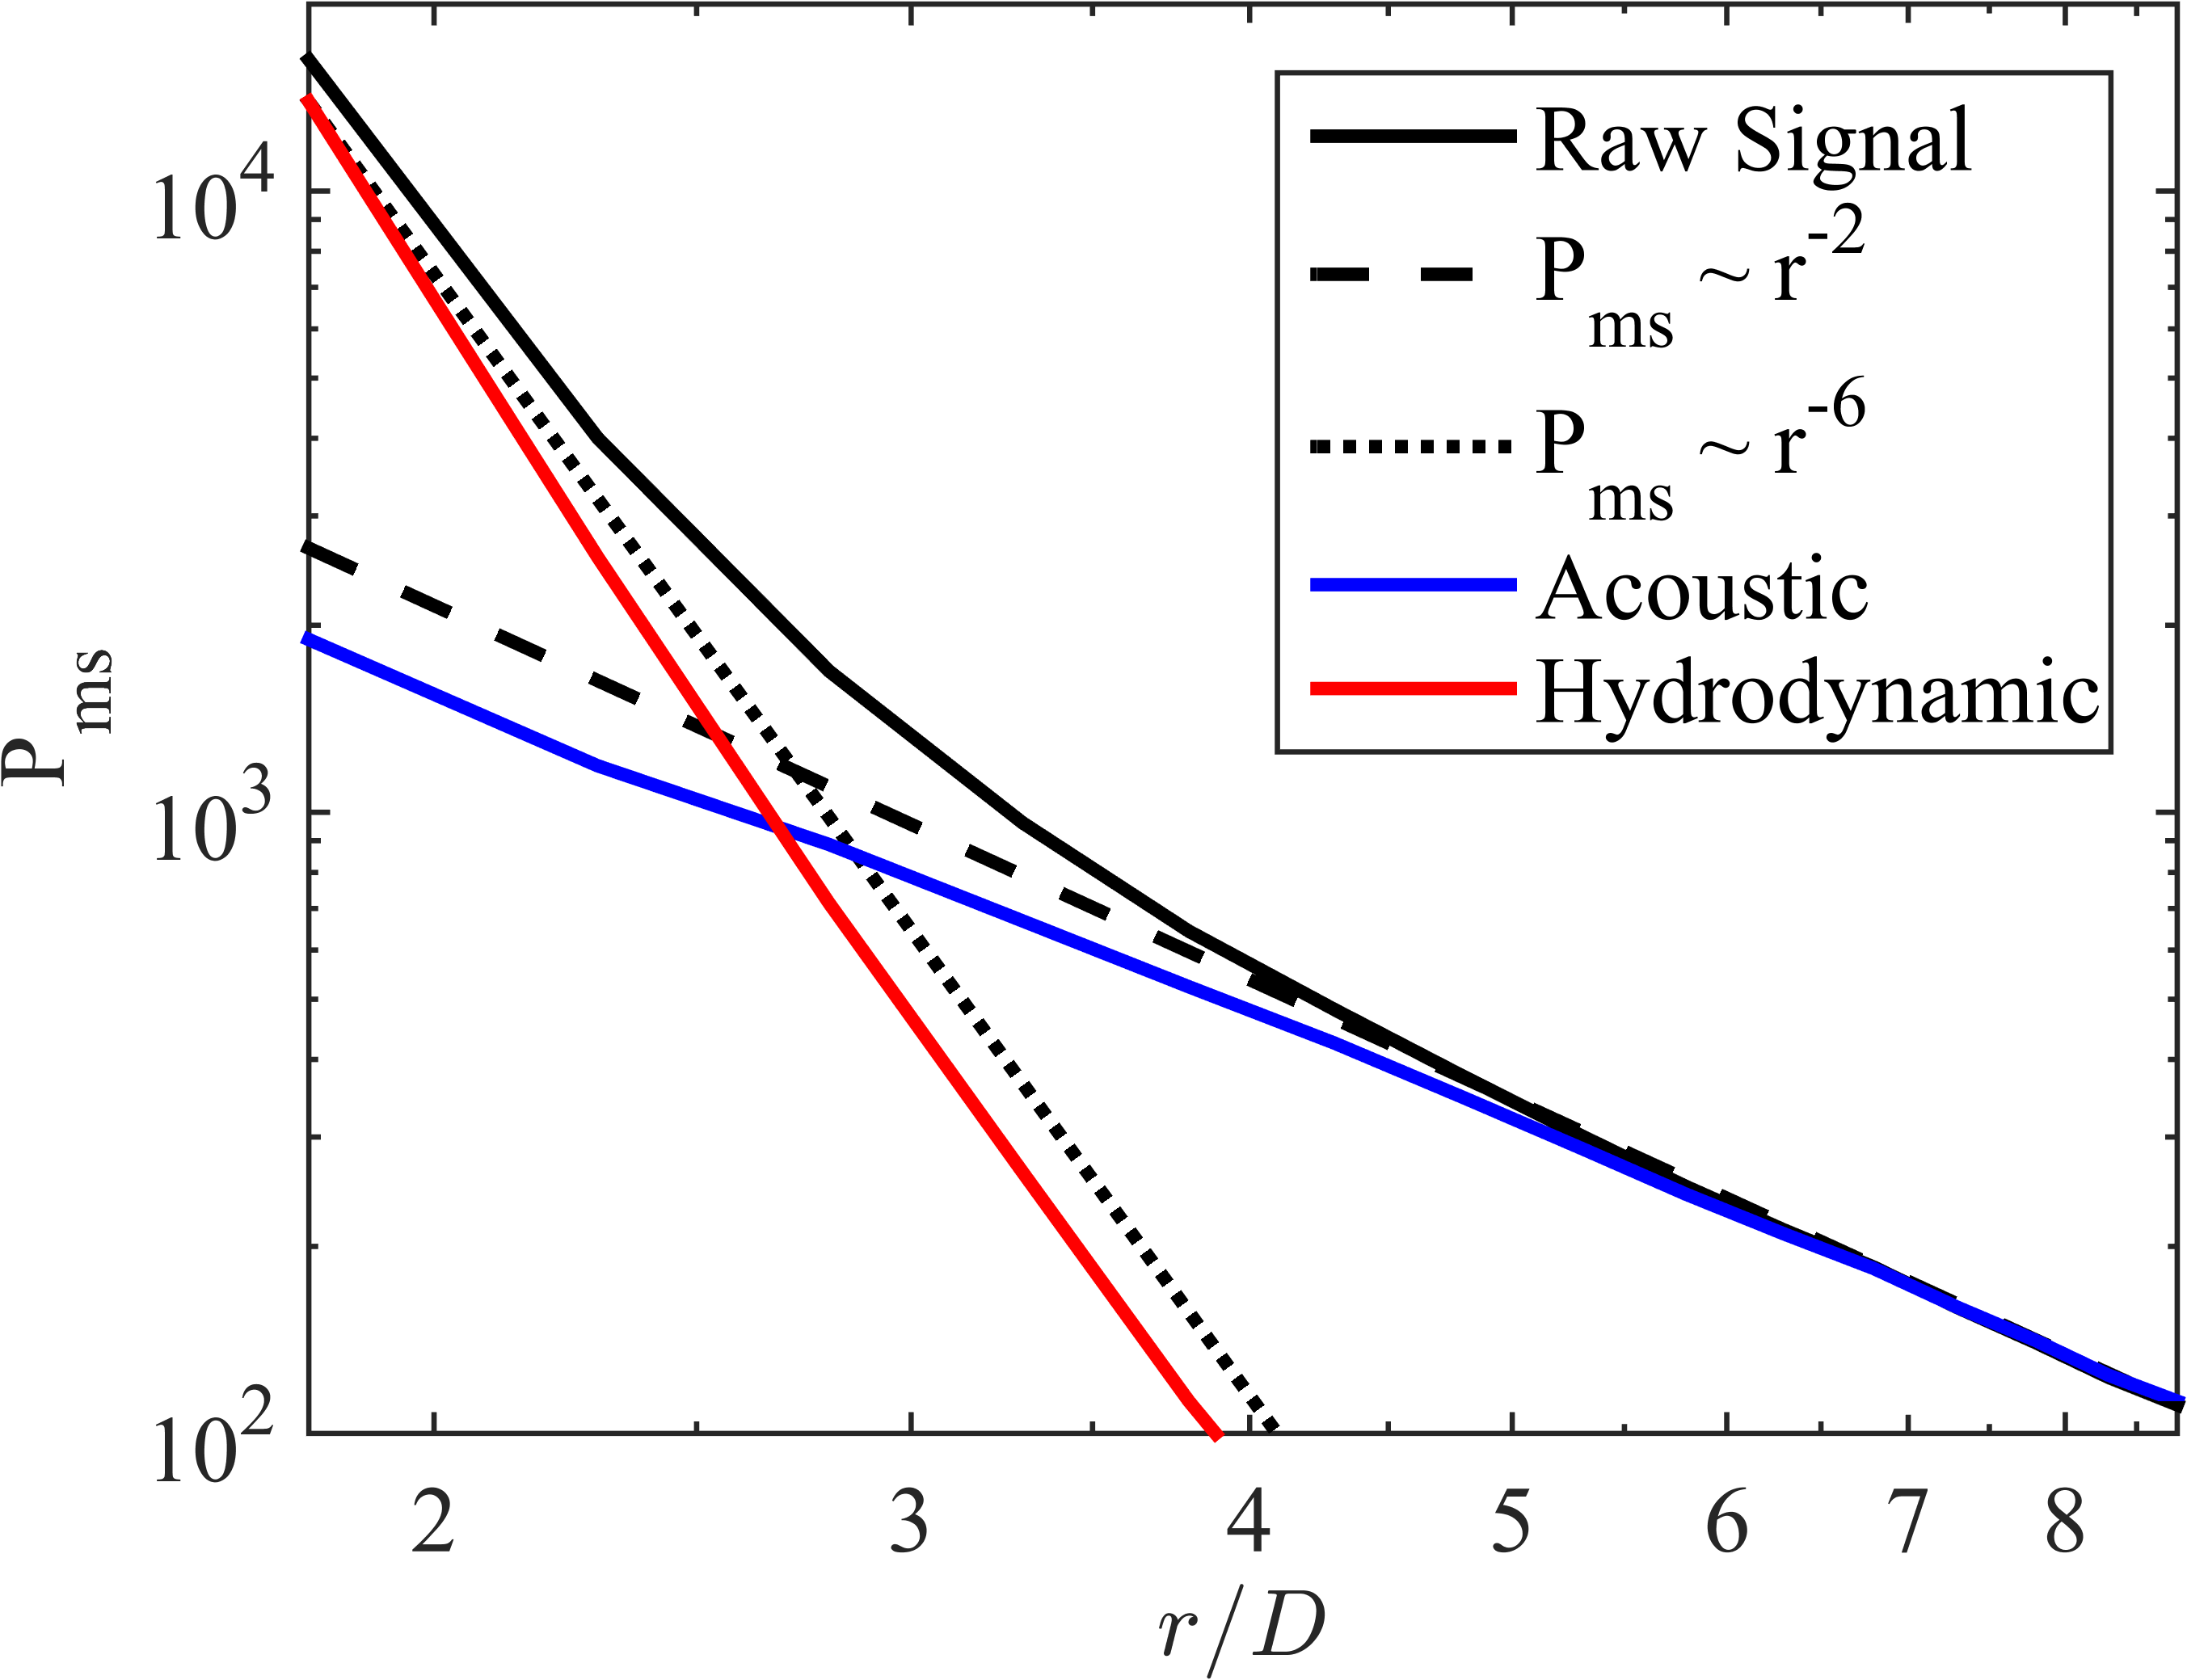
\includegraphics[width=4in]{Figures/ch3_validation_Pms_v2.png}
	\caption{Radial decay of the experimental signal compared against the theoretically-obtained and experimentally-measured decay rates for the acoustic and hydrodynamic components.}
	\label{fig:ch3_validation_Pms}
\end{figure}

Further insight into the veracity of the recovered acoustic and hydrodynamic fields may be obtained through analysis of the energy spectrum.
Like the radial decay rate of the pressure fluctuation intensities, Fourier analysis is inherently ill-suited for random processes and hence has been shown to miss certain important aspects of the jet noise process (e.g.,  intermittency). 
However, it has been used extensively throughout the aeroacoustic community for understanding the composition of both near-field pressure fluctuations as well as the acoustic far-field, to great success. 
Fundamental models in jet turbulence and aeroacoustics (e.g. the spectral decomposition of the irrotational near-field by Arndt \etal \citep{Arndt1997} and Tam’s similarity spectra for the acoustic far-field \citep{Tam1996}) analyze their respective phenomena in the Fourier domain.

Sample spectra taken at $x/D = 8, r/D = 2.2$ for the decomposed fields are shown in \fig{fig:ch3_validation_spectra}.
In the case of the hydrodynamic field (\fig{fig:ch3_validation_spectra_hydro}), the decomposed signal has been plotted against the raw near-field pressure spectrum as well as the $I \sim k^{-6.67}$ spectral decay rate in log space (with frequency/wavenumber) that was identified by Arndt \etal \citep{Arndt1997} as the decay rate for the inertial subrange of the irrotational near-field.
As one would expect for positions just outside the jet shear layer, the decomposition has identified the dominant spectral energy of the near-field as being hydrodynamic; the decomposed hydrodynamic field accounts for nearly the entire energy of the raw signal at low frequencies.
Beginning at moderate frequencies ($St_D \simeq 0.15$) a divergence between the raw irrotational near-field and the decomposed hydrodynamic field is observed, due to the increasing relative intensity of the acoustic field.
At frequencies above this threshold, the decomposed hydrodynamic field exhibits a decay rate that matches quite well with the theoretical prediction, over several orders of magnitude. 

The decomposed acoustic spectrum acquired at this same near-field position is compared against the far-field acoustic signal simultaneously acquired at a polar angle of $30^\circ$ in \fig{fig:ch3_validation_spectra_acoustic}.
The acoustic spectrum has been scaled in amplitude in order to account for spherical propagation of the waves; calculating the propagation distances requires an assumption on the acoustic source region, which is not initially known with certainty.
As will be discussed in more detail in \sect{sect:near_field_source_region}, by measuring the time delay in two-point correlations between the near-field microphones and the far-field microphone at $30^\circ$ the location of the dominant acoustic source region can be identified. 
In brief, the region just upstream of the end of the potential core ($x/D =4$) will be identified as the source region for the coherent large-scale structures in the jet; the current validation uses this location as the source region to scale the spectral amplitudes.
The signal at $x/D = 8, r/D = 2.2$ was chosen for this task as it lies roughly along a $30^\circ$ path from this assumed source region.
Additionally, the spectra were adjusted per ANSI S1.26 \citep{ANS1995} in order to account for atmospheric absorption of the (primarily high-frequency) acoustic waves due to propagation through a humid medium; the spectra shown here correspond to lossless propagation.
Lastly, the spectral peaks have been denoted by triangular markers at the top of the figure. 

It is found that the decomposed acoustic spectrum accurately reproduces the high-frequency portion of the far-field spectrum, which is unsurprising, given that the near-field spectra are dominated by acoustic fluctuations over this range of frequencies (though this does reinforce the accuracy of the amplitude-scaling used in the analysis).
Overall, the acoustic spectra extracted by the wavelet filter mirrors the far-field spectra quite well in terms of both spectral shape and amplitude, producing a `peaky' spectrum in contrast to the much more broadband raw irrotational near-field. 
The spectral peak occurs at nearly the same frequency as in the far-field, and is within 2 dB of the peak amplitude. 
The one major inaccuracy of the wavelet-based method is the failure to accurately reproduce the low-frequency spectral decay rate of the far-field spectrum. 
\begin{figure}
	\centering
	\begin{subfigure}{.5\textwidth}
		\centering
		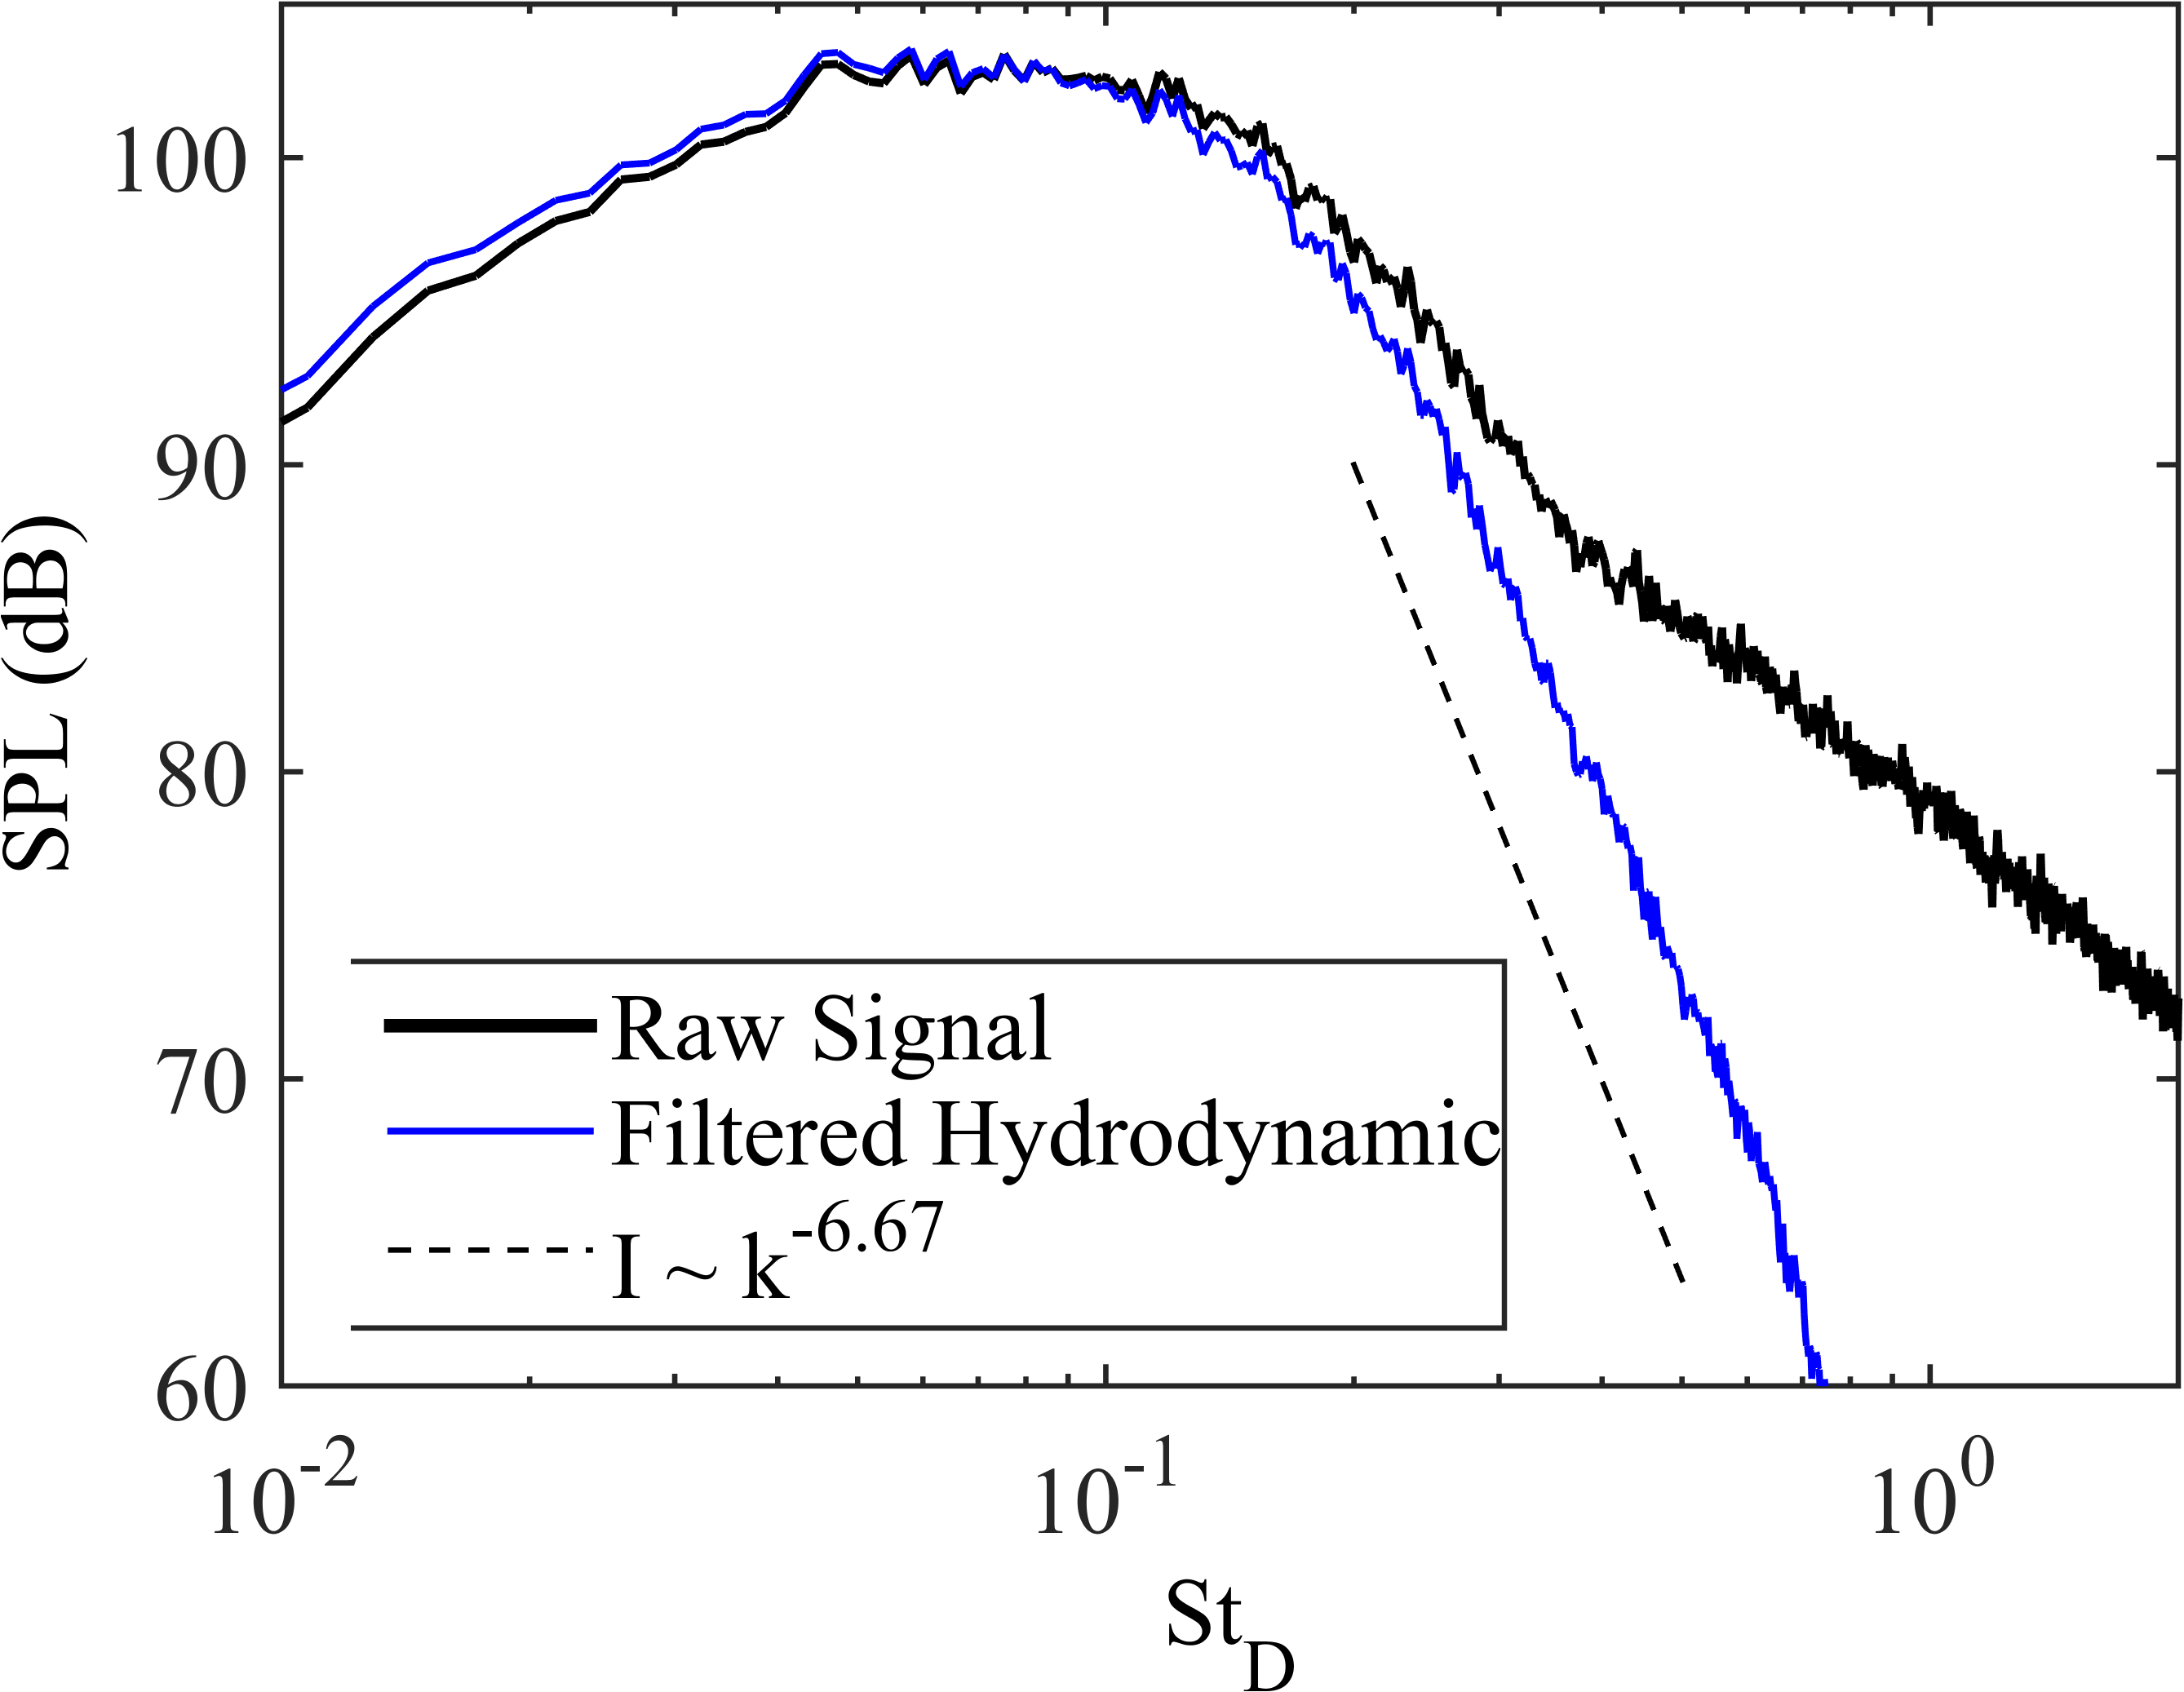
\includegraphics[width=0.95\linewidth]{Figures/ch3_validation_spectra_hydrodynamic}
		\caption{Hydrodynamic Decomposition}
		\label{fig:ch3_validation_spectra_hydro}
	\end{subfigure}%
	\begin{subfigure}{.5\textwidth}
		\centering
		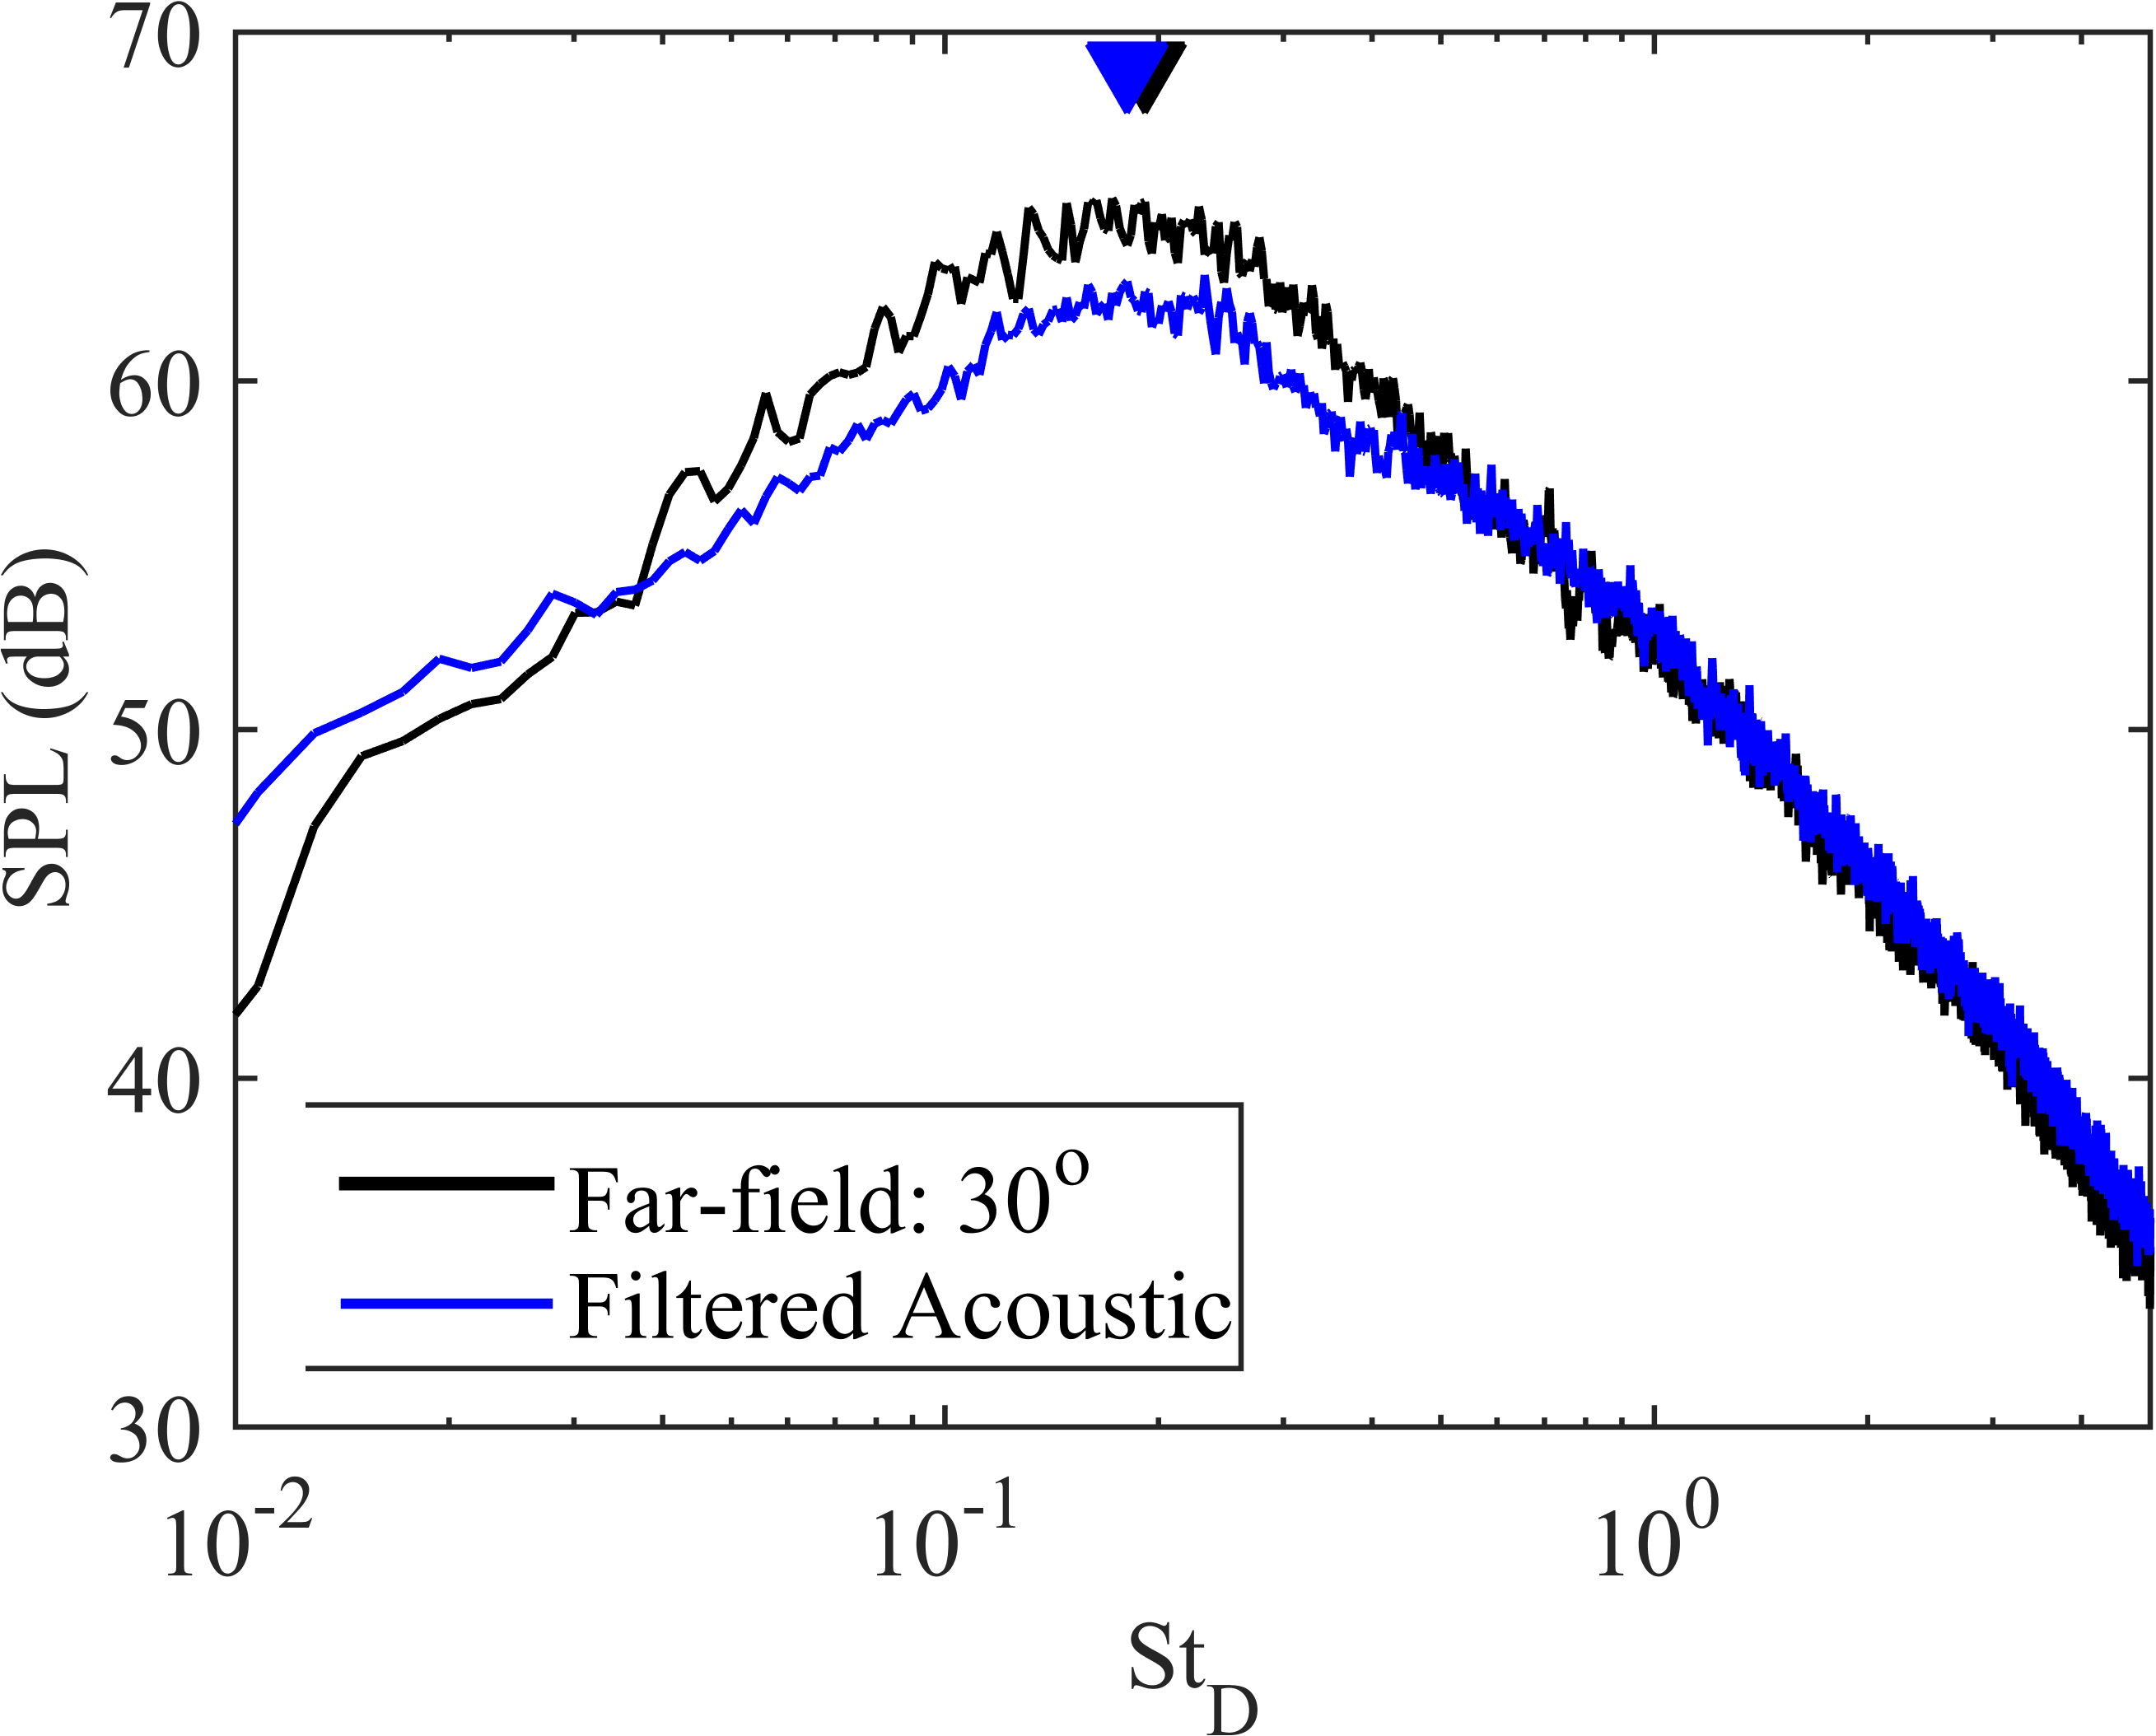
\includegraphics[width=0.95\linewidth]{Figures/ch3_validation_spectra_acoustic}
		\caption{Acoustic Decomposition}
		\label{fig:ch3_validation_spectra_acoustic}
	\end{subfigure}
	\caption{Spectral comparison of decomposed hydrodynamic field compared against the raw near-field signal (a) and decomposed acoustic field compared against the far-field acoustic signal at $30^\circ$. In both cases, the near-field signal was acquired at $x/D = 8, r/D = 2.2$}
	\label{fig:ch3_validation_spectra}
\end{figure}

As a final method of validation, the decomposed fields for the excited jet were analyzed in the time domain by phase-averaging.
As has been pointed out by numerous other researchers \citep{Cavalieri2010,Camussi1997,Kearney-Fischer2013,Hileman2005}, the turbulent jet and resultant acoustic field are highly intermittent phenomena. 
An illustration of this behavior can be found in \fig{fig:ch3_wavelet_spectrum}, where the wavelet power spectrum of the far-field at $30^\circ$ has been plotted as a function of (pseudo) Strouhal number and time for the unforced jet; this can be compared against the Fourier power spectrum presented in \fig{fig:ch3_validation_spectra_acoustic}. 
As with the Fourier analysis, wavelet analysis demonstrates that the baseline jet radiates to the far-field over a broad range of Strouhal numbers, with the dominant energy occurring for $St_{DF} \simeq 0.15$. 
However, the far-field is found to be composed of temporally- and frequency-localized bursts of energy – far from the stationary field that Fourier analysis assumes. 
Clearly, this intermittent behavior needs to be recovered in the near-field by the decomposition process; something which may be evaluated with the aid of LAFPA excitation.
\begin{figure}
	\centering
	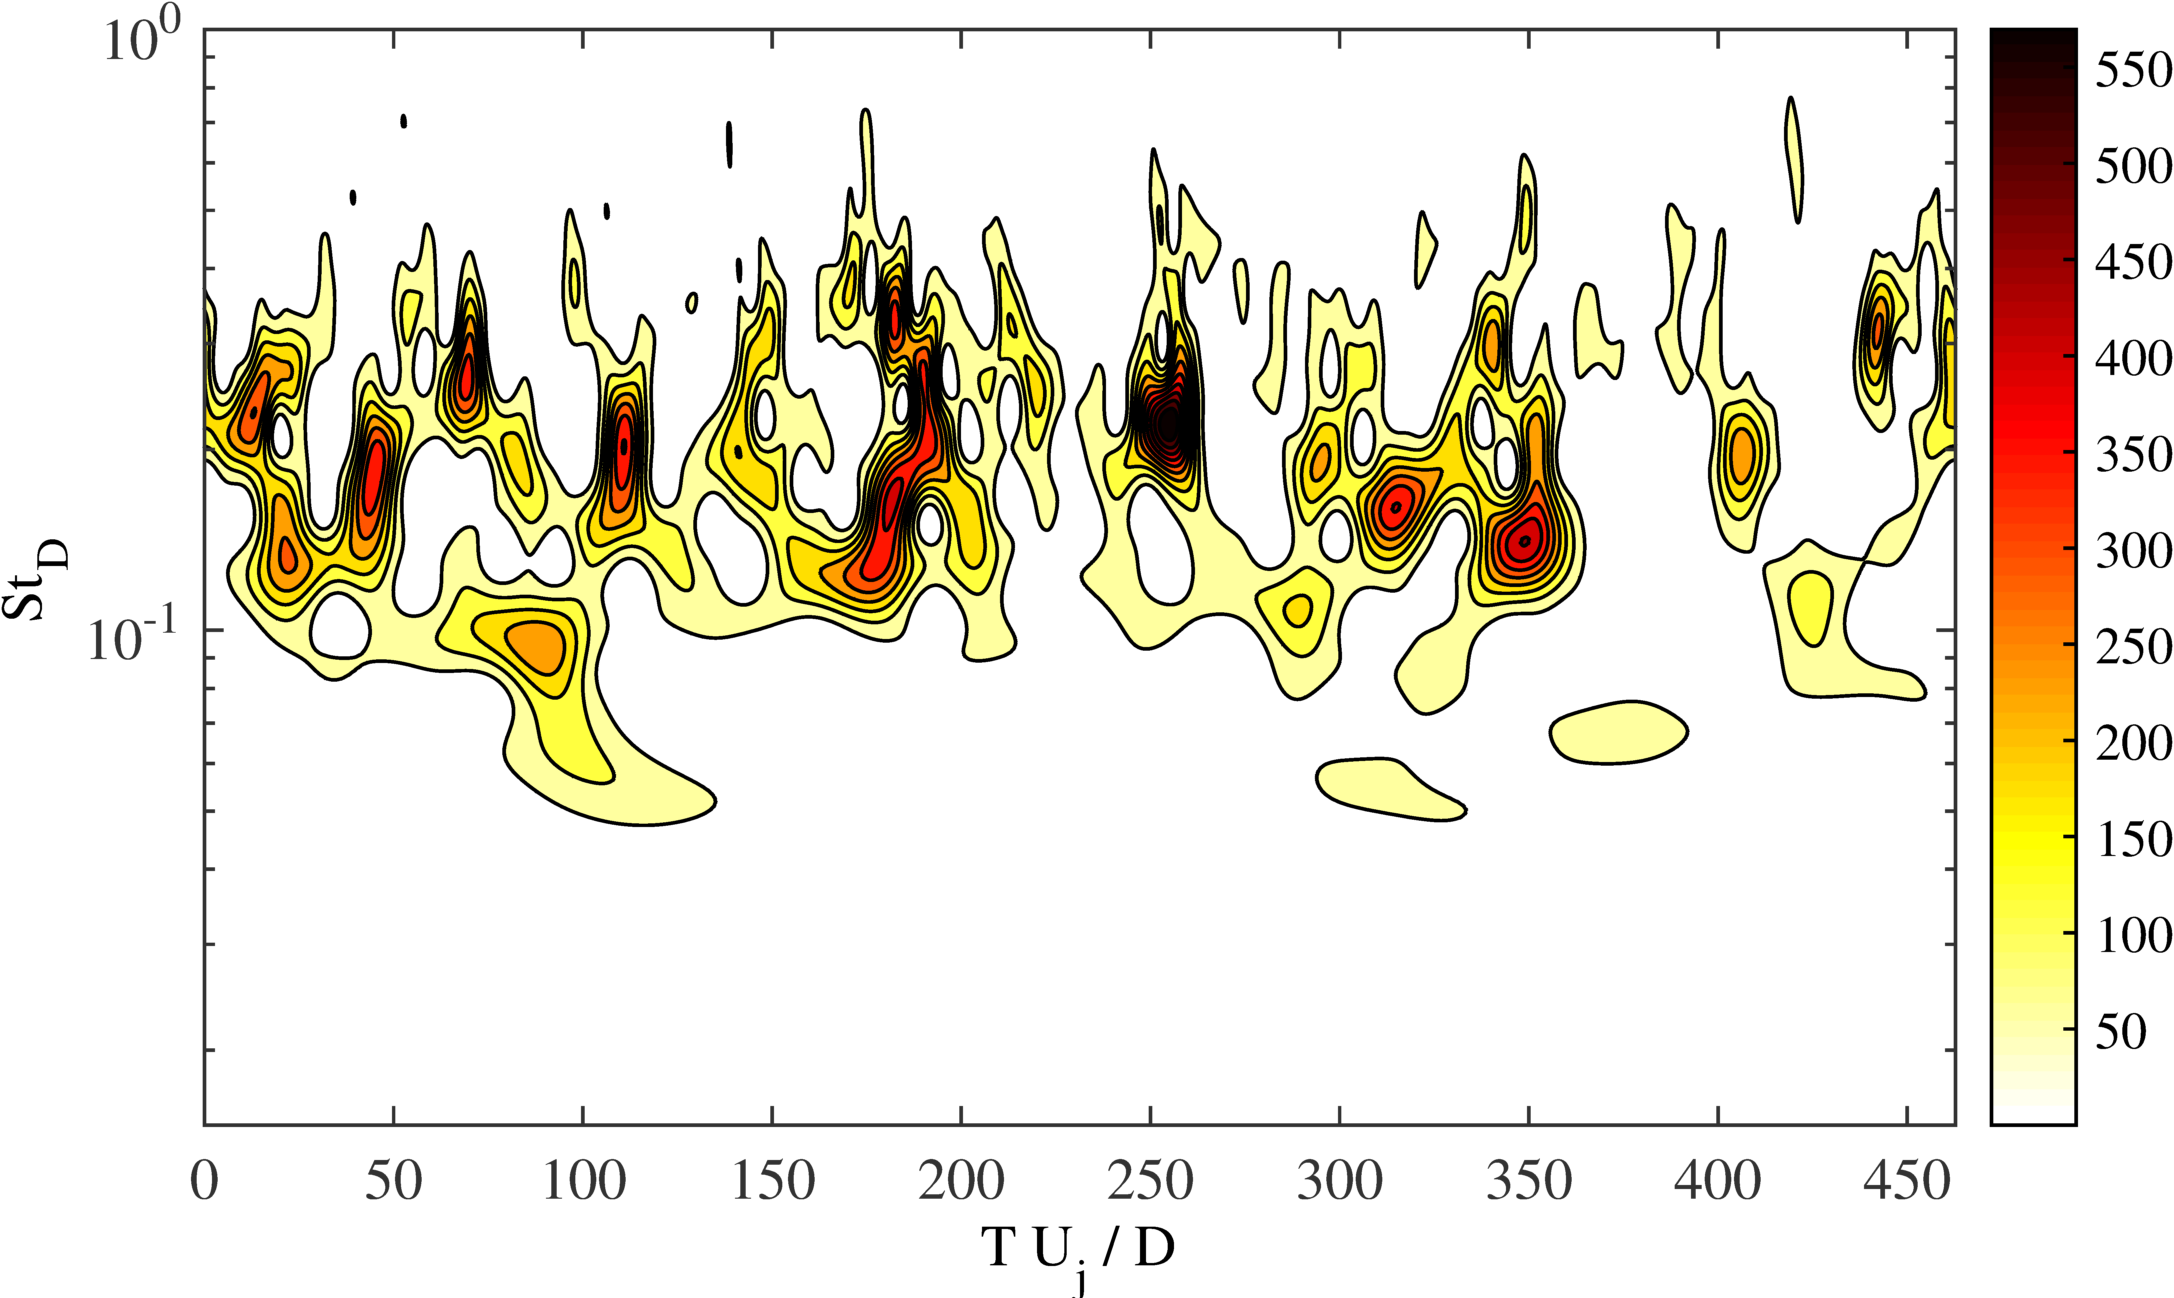
\includegraphics[width=4in]{Figures/ch3_wavelet_spectrum.png}
	\caption{Wavelet power spectrum in the acoustic far-field at $30^\circ$ for the natural jet.}
	\label{fig:ch3_wavelet_spectrum}
\end{figure}

As before, the decomposed acoustic signal at $x/D = 8, r/D = 2.2$ was propagated to the far-field at $30^\circ$ by scaling the amplitude according to $I \sim r^{-2}$; the phase-averaged signal was also shifted in time based on the ambient speed of sound in order to account for the propagation delay. 
Results of this procedure can be found in \fig{fig:ch3_validation_phavg} for the jet excited at $St_{DF} = 0.05$. 
For illustrative purposes, results computed using the more standard Fourier-based decomposition method have also been included here.
Both the Fourier and wavelet methods identify a distinct waveform which matches quite well with the waveform observed in the far-field, though with some discrepancies. 
The wavelet-method produces a slightly more accurate peak amplitude and event temporal extent. 
The most significant difference between Fourier and wavelet methods is the existence of severe ringing (caused by Gibbs’ phenomena) observed in the Fourier results just preceding the acoustic event. 
This phenomena persists even when the events are now highly periodic, (not shown here for brevity). 
\begin{figure}
	\centering
	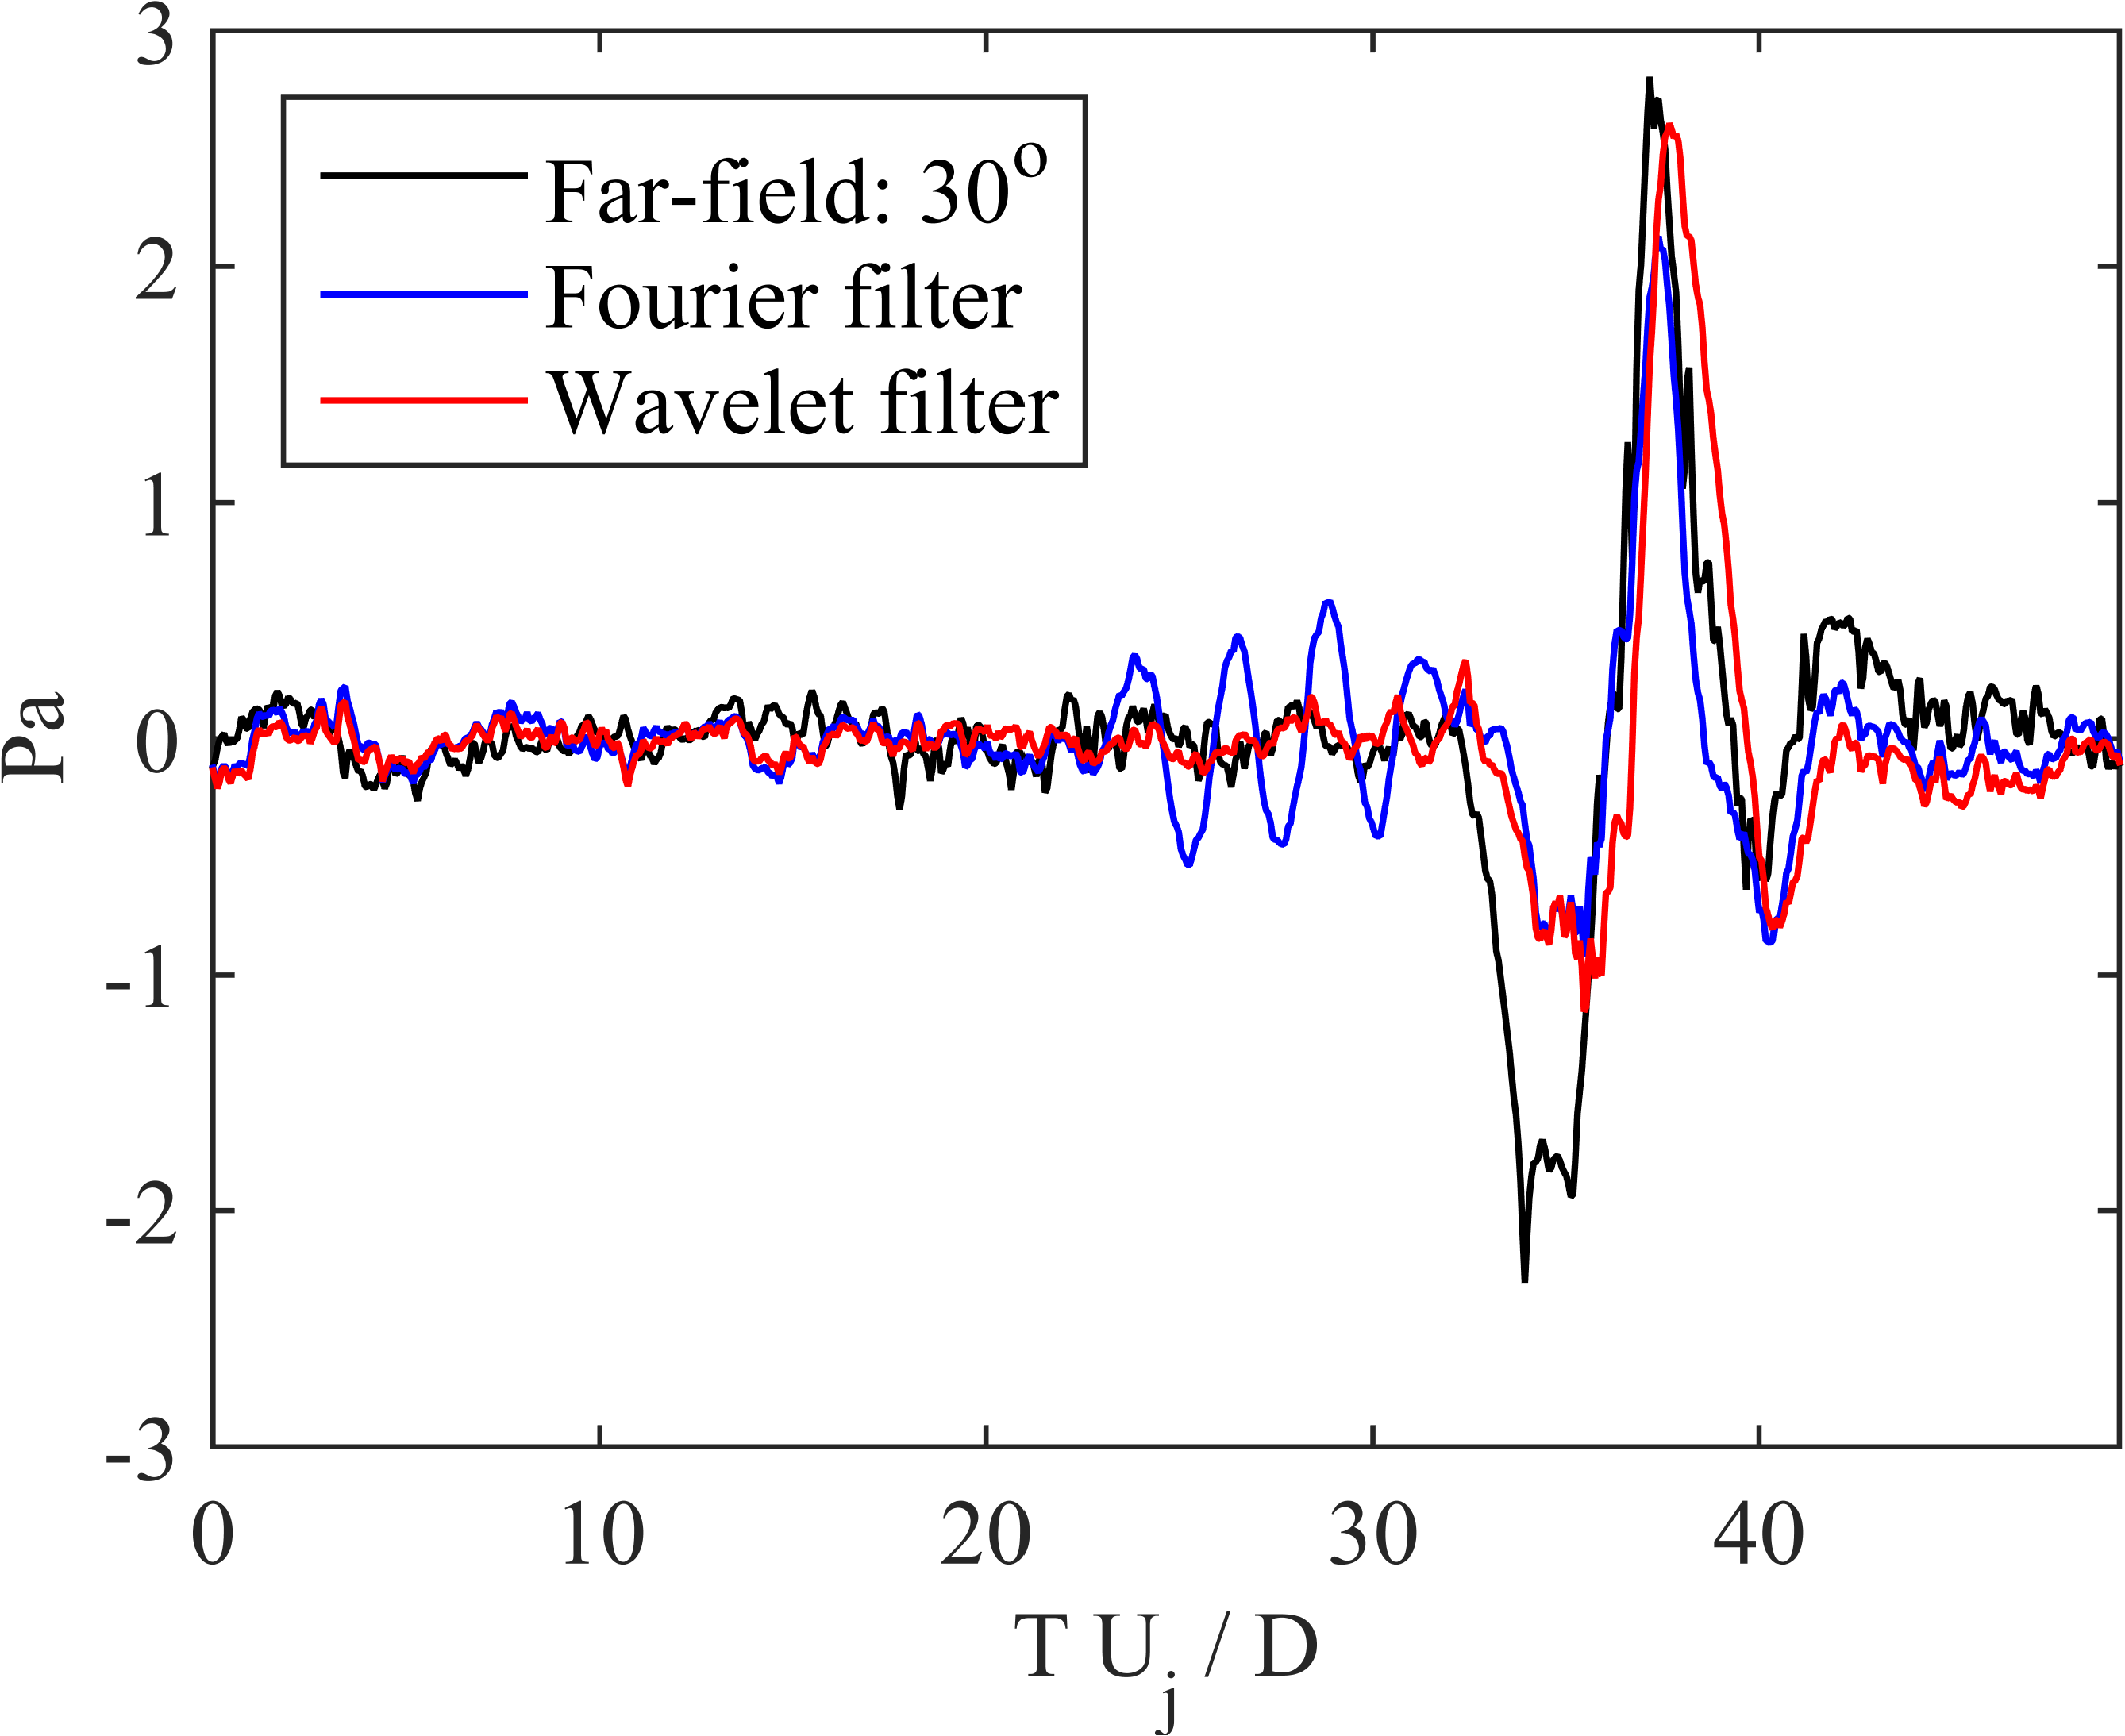
\includegraphics[width=4in]{Figures/ch3_validation_phavg.png}
	\caption{Comparison of phase-averaged waveforms produced by excitation at $St_{DF} = 0.05$. As before, the near-field signal was acquired at $x/D = 8, r/D = 2.2$}
	\label{fig:ch3_validation_phavg}
\end{figure}

In the case of a subsonically-convecting jet, the conceptual basis behind the Fourier decomposition algorithm is not in error (excluding the periodicity assumed by the Fourier transform). 
Instead, the practical requirements of discretely sampled microphones spanning a finite region in space, in addition to noise in the data acquisition, lead to numerical artifacts in the reconstructions. 
The Fourier transform required an extensive axial array of microphones (16 microphones spanning $21D$ in the current study) in order to accurately represent the pressure fluctuations (the array was originally designed with the intent of using the  Fourier-based decomposition).  
This is because the basis functions (trigonometric function) used in the Fourier transform are not physically representative of the physical phenomena under study. 
As discussed previously, the turbulent jet (and resultant acoustic field) is highly intermittent. 
Even with the excitation producing regular large-scale structures, these, as well as the resultant acoustic emissions, exist as temporally and spatially localized energy bursts, rather that space-filling sinusoidal waves (as assumed by the Fourier transform). 
It has been shown that by using a temporally/spatially localized fluctuation as a basis, the wavelet transform compresses the information in a turbulent field much more efficiently (and accurately) than the Fourier transform \citep{Farge1992}.

Though there are some relatively minor discrepancies between the expected acoustic near-field and the one produced by the spatio-temporal wavelet filter, overall the results are promising.
The decomposition algorithm is extracting hydrodynamic and acoustic fields which accurately reproduce the expected radial and frequency decay rates per theoretical analysis over the large domain investigated in this work (both in terms of spatial and frequency/wavenumber extent).
Additionally, this accuracy is also not just a statistical phenomenon, as the decomposition algorithm is also found to accurately identify and reconstruct strongly-energetic, localized bursts of energy in the constitutive fields. 
Based on these results, the author felt confident that the decomposed acoustic field produced by the spatio-temporal wavelet filter was highly representative of the true acoustic near-field.

\section{Identifying the Acoustic Source Region}
\label{sect:near_field_source_region}
Correlation analysis has long been used by researchers as a simple tool to quantify the relationship between two or more signals separated either by space or time.
In its simplest form, two-point correlations measure the similarity and phase delay by a linear convolution of two signals.
It is perhaps unsurprising then that two-point correlations are ubiquitous in fluid dynamics research.
In this work, they will be used to better understand the relationship between the near-field dynamics and the acoustic radiation reaching the far field at aft angles.
Correlations were computed (using the measured signals, as opposed to the phase-averaged waveforms) between each microphone in the near field and the far-field microphone at $30^\circ$. 
The correlations were then examined in the spatio-temporal domain, which showed distinct regions of positive and negative correlation spanning several jet diameters and flow time scales.
\begin{figure}
	\centering
	\begin{subfigure}{.5\textwidth}
		\centering
		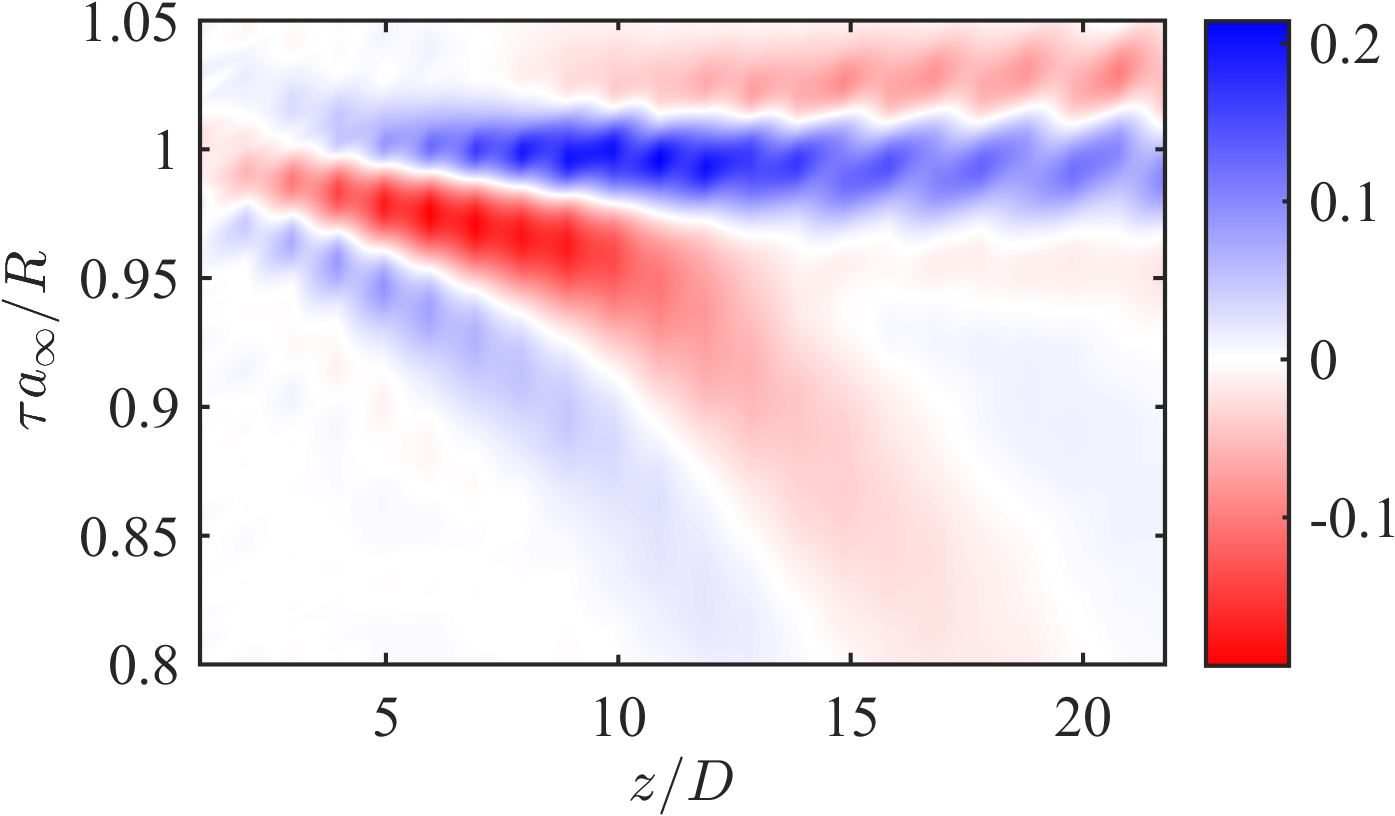
\includegraphics[width=0.95\linewidth]{Figures/ch3_St000_xcorr_r1D.png}
		\caption{$r/D = 1.2$}
		\label{fig:ch3_fullxcorr_r1D}
	\end{subfigure}%
	\begin{subfigure}{.5\textwidth}
		\centering
		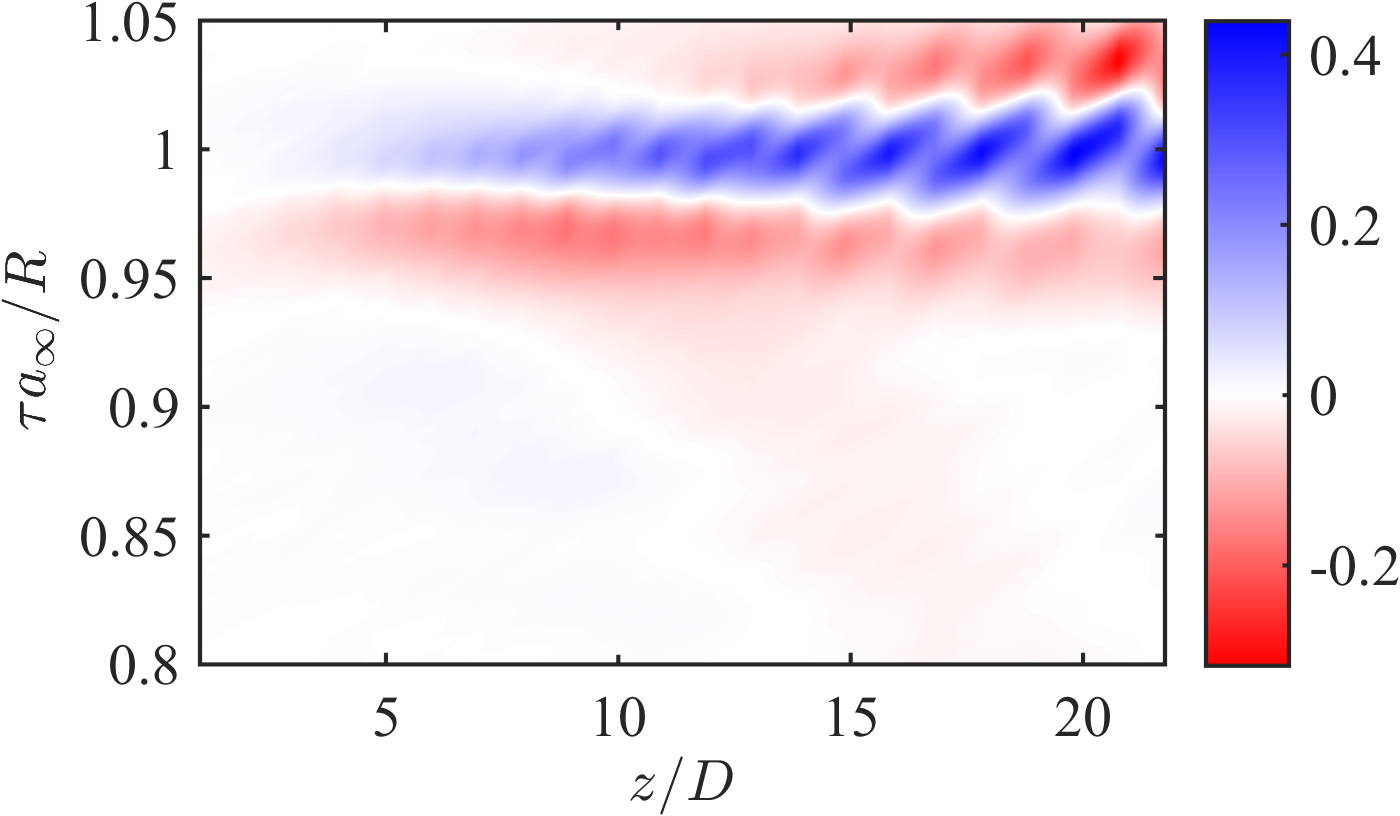
\includegraphics[width=0.95\linewidth]{Figures/ch3_St000_xcorr_r4D.png}
		\caption{$r/D = 4.2$}
		\label{fig:ch3_fullxcorr_r4D}
	\end{subfigure}
	\caption{Normalized two-point correlations for the natural jet between the near field and the far field at $30^\circ$ for two microphone array positions.}
	\label{fig:ch3_fullxcorr}
\end{figure}

This behavior can be observed in \fig{fig:ch3_fullxcorr}, where the two-point correlations between the near-field and the far-field at $30^\circ$ for two microphone array positions (starting at $x/D = 1, r/D = 1.20$ and $x/D = 1, r/D = 4.20$) have been plotted.
The time lag, $\tau$, in the figures have been non-dimensionalized by the ambient speed of sound, $a_\infty$, and $R$, the distance from each near-field microphone to the far-field microphone (note that this results in an ordinate that is scaled separately along the abscissa, due to the dependence of the axial position on $R$).
Therefore, $\tau a_\infty /R = 1$ corresponds to the time delay for an acoustic wave to travel directly from the near-field microphone to the far-field microphone.

Near the jet shear layer (\fig{fig:ch3_fullxcorr_r1D}), four distinct correlation regions can be observed: two positive, two negative; one strong and one weak for each. 
The first correlation regions, the strong-negative and weak-positive, are noticeable beginning at the most upstream microphone and reach their peak values around $5 < x/D < 10$, decaying significantly beyond that.
The slopes of these regions indicate propagation velocities noticeably below the sonic velocity; in the upstream region, they roughly match with the measured convective velocity of the large-scale structures ($U_c \simeq 0.7 U_j$ as measured by two-point correlations between subsequent near-field microphones, see Crawley \etal \citep{Crawley2015} for additional details) in the upstream region of the jet, and slowly decelerate downstream.
Similar behavior was observed by Bogey \& Bailley \citep{Bogey2007}, who noted that two-point correlations between the flow-field and acoustic near-field in a simulated jet produced strong positive correlation regions which peaked at the end of the potential core and which followed the convection of the large-scale structures.
Conversely, the strong-positive and weak-negative correlation regions exhibit propagation velocities that match well with the ambient speed of sound. 
These correlation regions start from almost negligible values upstream, strongly amplify near and just beyond the end of the potential core, and decay gradually in the most downstream region.

As the microphone array is moved radially outwards (\fig{fig:ch3_fullxcorr_r4D}), the strong-negative and weak-positive correlation regions quickly decay to negligible values and all observable correlation regions begin to match the expected time-of-arrival for sonically-traveling waves. 
The distinctly different propagation velocities and axial and radial evolutions of the two pairs of correlation regions indicate that these correspond to different physical phenomena.
The strong-negative and weak-positive correlation regions observed near the jet shear layer are associated with the large-scale structures themselves, rather than acoustic phenomena. 
The positive and negative correlation regions are likely associated with the braid and core regions of the large-scale structure as they convect through the shear layer. 
The low-pressure core region of the vortex produces a positive correlation value with the far-field acoustic due to the phase inversion of the acoustic waveform at low polar angles (\fig{fig:ch3_nearfield}). 
At this radial location, the dominant energy measured by the microphone array is acoustic, owing to the strong decay of the hydrodynamic field with radial distance from the jet \citep{Arndt1997}.
Though they have not been included here for brevity, the two-point correlations in the excited jet cases show similar behavior, albeit with enhanced correlation levels particularly for the large-scale structure related regions. 

This relationship becomes even more clear when just the acoustic component of the near-field is considered during computation of the two-point correlations, rather than the full irrotational near-field. 
Gone entirely now are the correlation regions with subsonic propagation velocities, even at the closest microphone array positions, as can be seen in \fig{fig:ch3_St000_acoustic}.
Instead, a single positive correlation region corresponding to sonically-propagating waves exists over the entire domain with significantly enhanced correlation over the full field results. 
In fact, the results found here for the acoustic component along the first microphone array position are nearly identical to those for the full field response at the further away array positions (\fig{fig:ch3_fullxcorr_r4D}), which were dominated by acoustic, rather than hydrodynamic, energy.
\begin{figure}
	\centering
	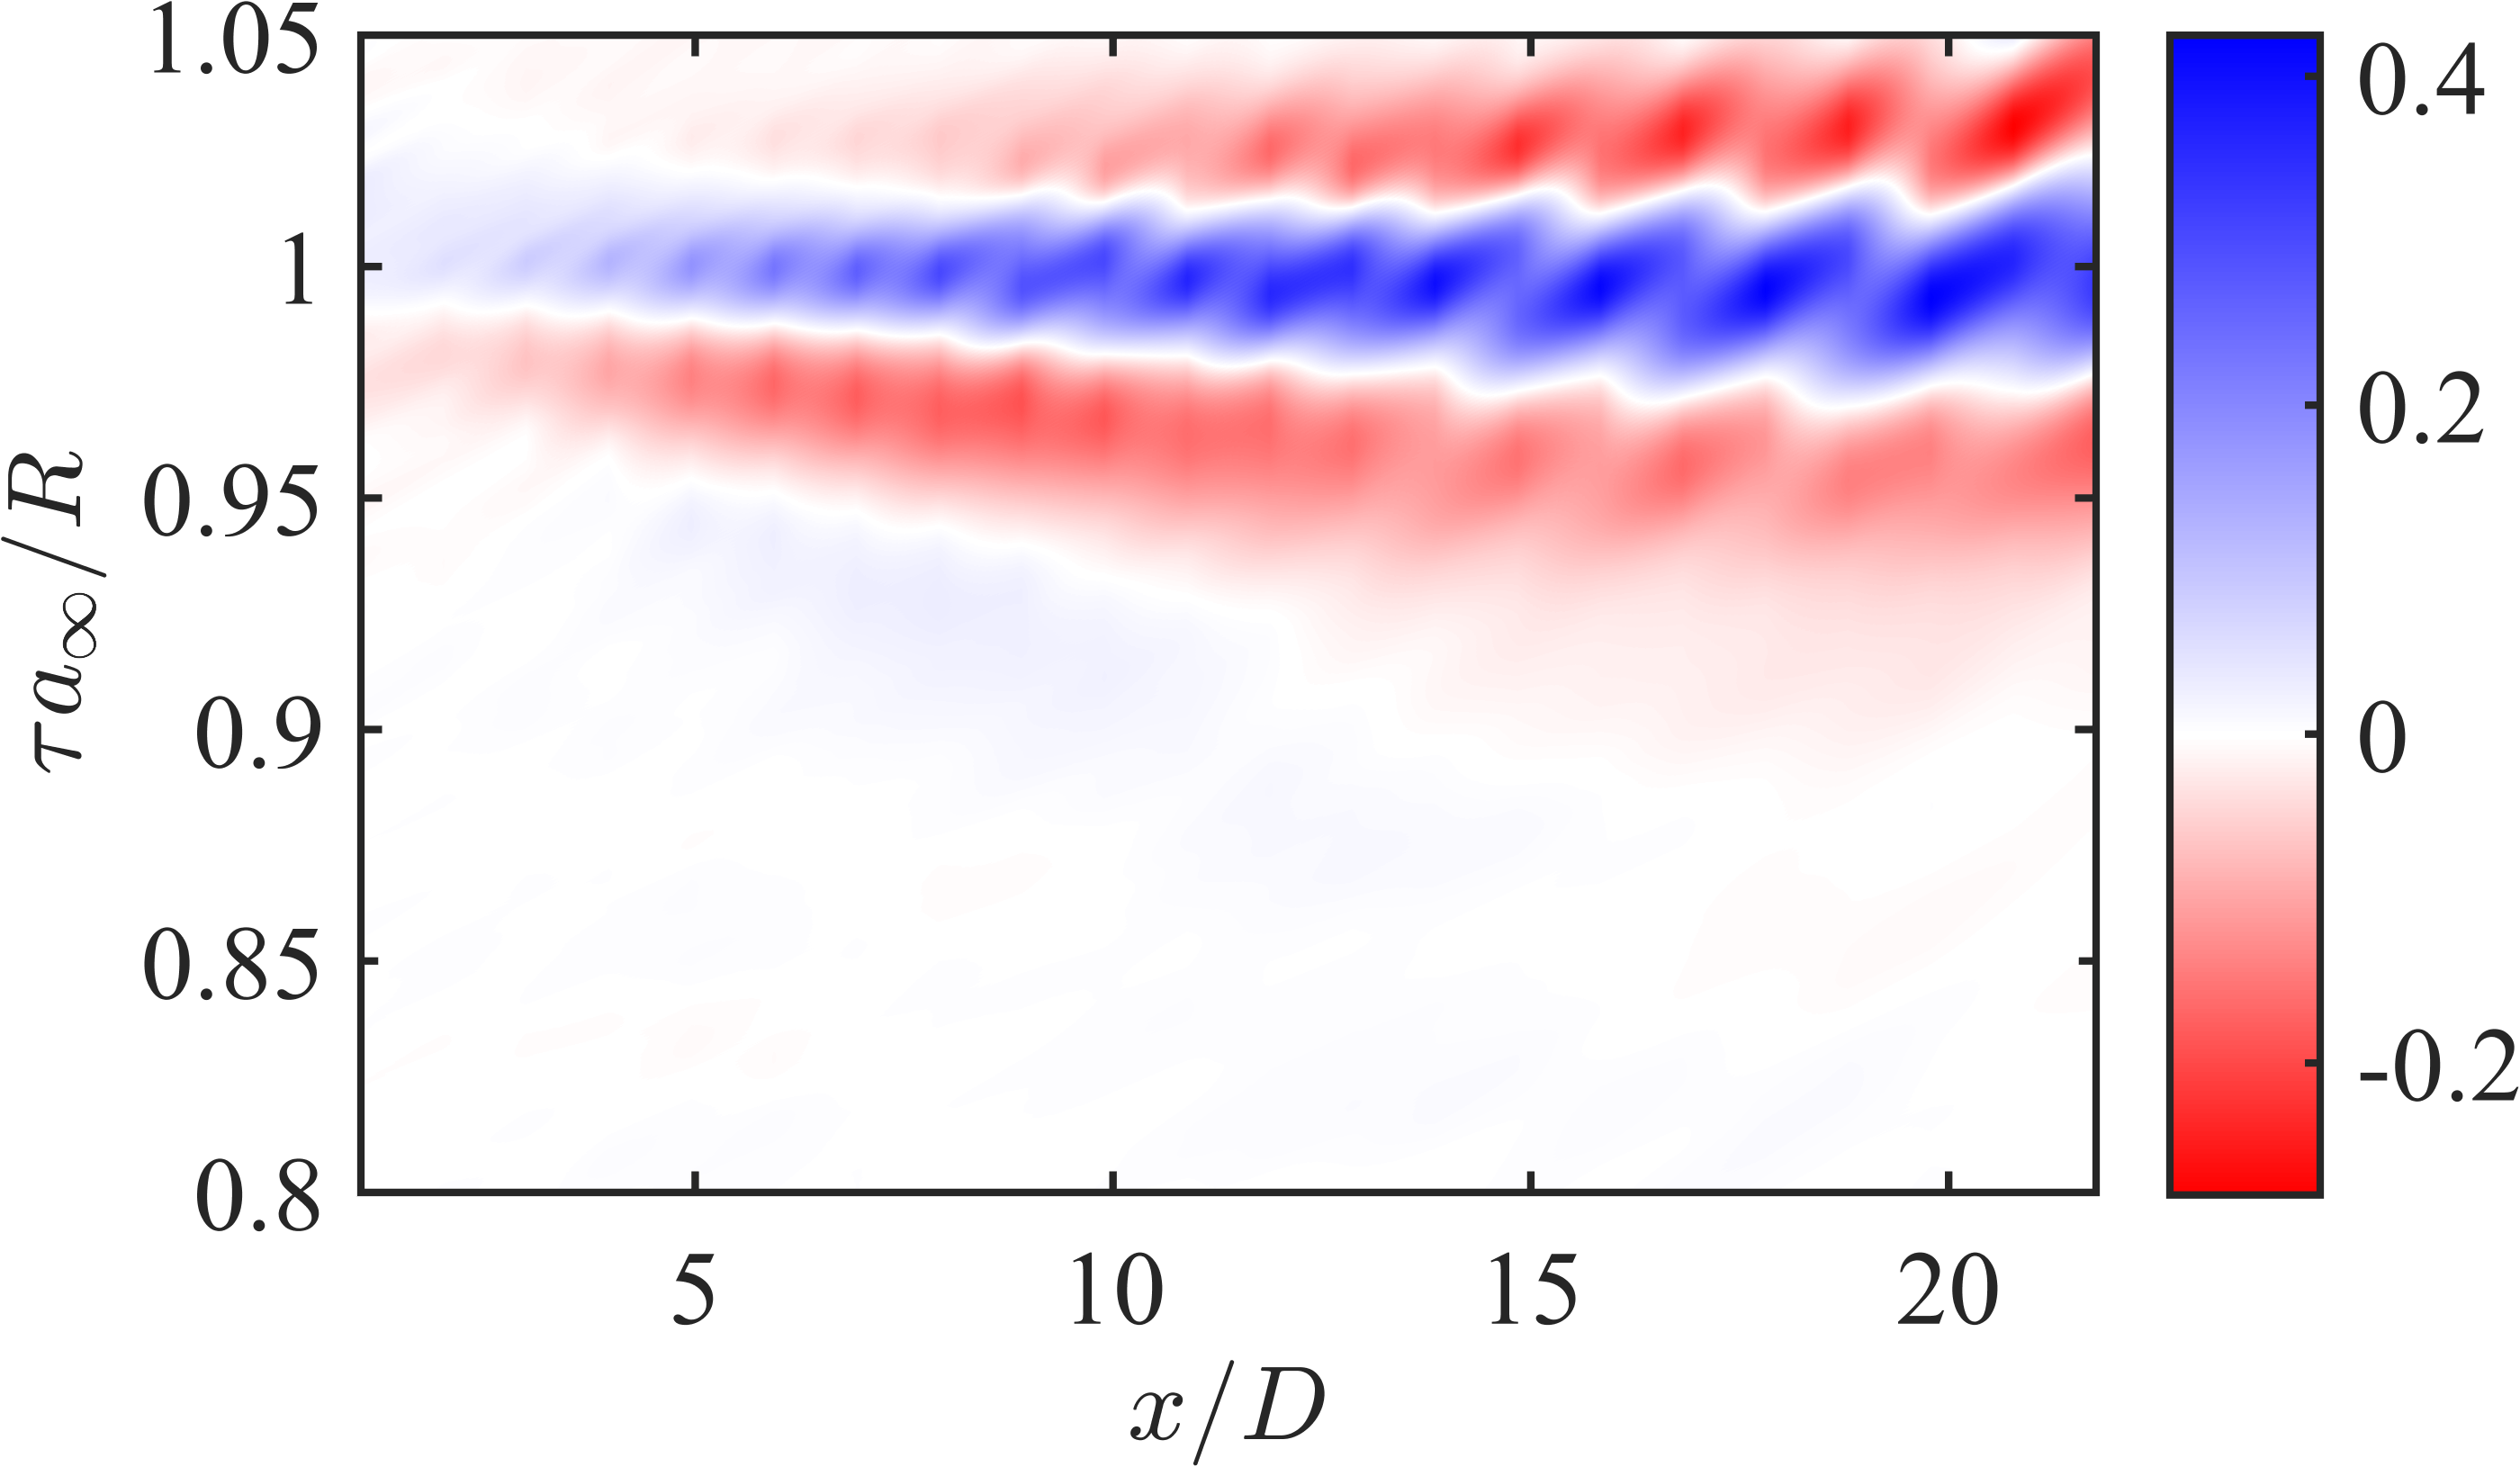
\includegraphics[width=4in]{Figures/ch3_St000_xcorr_acoustic.png}
	\caption{Normalized two-point correlations for the natural jet between the acoustic component of the near field and the far field at $30^\circ$ for microphone array position starting at $x/D = 1, r/D = 1.2$. }
	\label{fig:ch3_St000_acoustic}
\end{figure}

We can now use the correlations of the decomposed near-field in order to identify the acoustic source region, at least in a rough sense, by comparing the time lag at which the greatest correlation is achieved against expected times-of-arrival for different propagation paths.
A schematic of these propagation paths is provided in \fig{fig:ch3_ToA}.
The first expected time of arrival, $\tau_a$, corresponds to the expected time lag for an acoustic wave traveling directly from the noise source to the near-field microphone and on to the far-field microphone and hence, the noise source region lies along the axis created by the near-field and far-field microphones.
Another expected time-of-arrival can be constructed by assuming the source region is stationary in space; from simple geometric considerations of the distance from the assumed source region to the near-field and far-field microphones, the time lag, $\tau_s$, between the arrival of an acoustic wave at both microphones can be computed.
The stationary source region is of course not known \textit{a priori}, but is set by the author subsequent to the computation of the two-point correlations.

For simplicity, density and convection effects on the acoustic wave as it travels through the jet shear layer have been neglected in this analysis. 
By necessity, it has been assumed that the acoustic radiation in the jet is dominated by $m = 0$ azimuthal Fourier mode (the near-field and far-field microphone arrays are not at the same azimuthal angle with respect to the nozzle). 
This assumption is easily justified in the excited jets, where the actuators have been fired in phase. 
While the near-field pressure and acoustic radiation towards aft polar angles in a natural, high Reynolds number jet is a combination of numerous azimuthal Fourier modes, previous researchers have found these fields to be dominated by the axisymmetric mode \citep{Arndt1997,Hall2006,Koenig2013,Juve1979}.
\begin{figure}
	\centering
	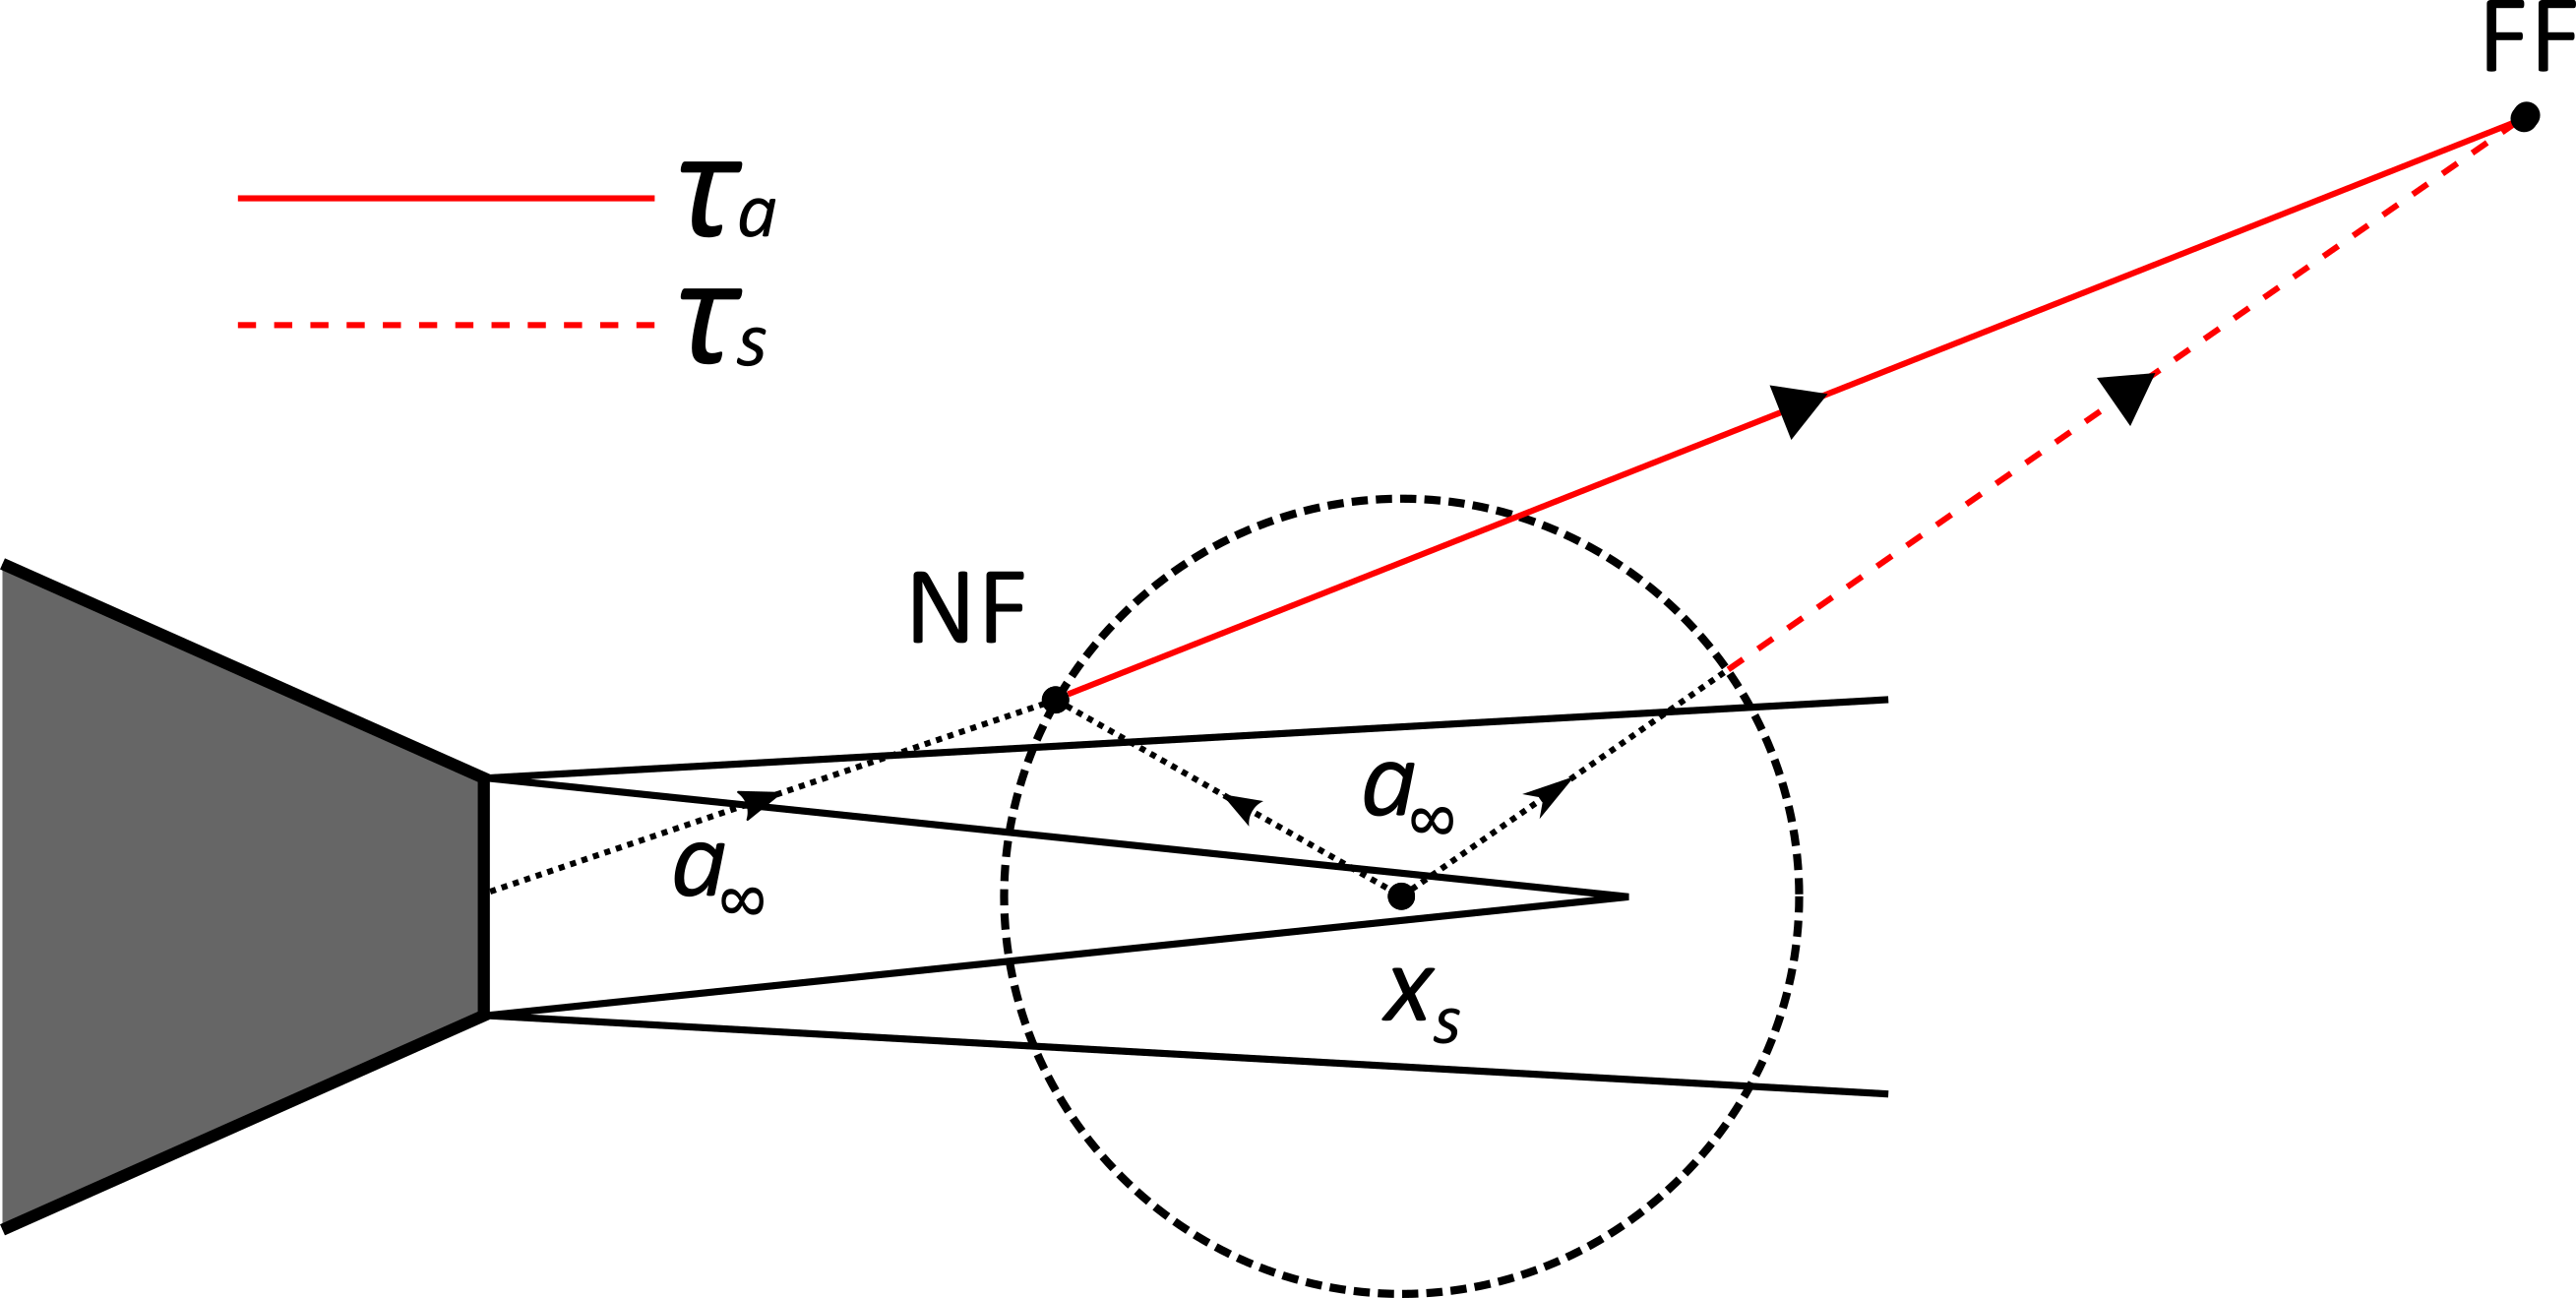
\includegraphics[width=4in]{Figures/ToA_tau.png}
	\caption{Expected times of arrival for on-axis acoustic propagation, $\tau_a$, and off-axis acoustic propagation, $\tau_s$ from a stationary source region centered at $x_s$.}
	\label{fig:ch3_ToA}
\end{figure}

Here, the acoustic source region was assumed to be located at $x_s /D = 4$, which is just upstream of the end of the potential core in the unforced jet. 
(Please note that this analysis is not meant to imply that the source region is located at a specific, fixed point – it is merely a convenient way of understanding the propagation paths.)
Similar behavior is observed between the natural jet and the excited cases in \fig{fig:ch3_xcorrOA}; note that due to numerical discrepancies at the domain boundaries (see Torrence \& Campo \citep{Torrence1998} for a discussion of the `cone of influence' of wavelet coefficients and the effect thereof), the correlation values have been truncated at the most upstream and downstream microphones.
For the impulsively-excited jet, nearly identical correlation regions are observed between the excited and natural jet; in the periodically-excited jet continuous oscillations occur throughout time due to the similarity of continuously-generated large-scale structures and resultant acoustic radiation.
In the upstream region of the jet, the peaks of the positive correlation region match $\tau_a$ nearly exactly. 
In the downstream region, $\tau_a$ begins to increasingly over-predict the time lag for the maximum correlation. 
On the other hand, $\tau_s$ tracks the time lags for the peak correlation consistently over the downstream region, but not the upstream region. 
The results found here appear to indicate that the dominant acoustic radiation reaching the far-field aft angles is being generated over an extended region of the jet mixing layer, roughly $x/D \leq 4$, which is just upstream of the time-averaged end of the potential core in the natural jet.
This is not too dissimilar from the findings of other researchers, who have suggested that the acoustic source region lies just \textit{downstream} of the end of the potential core \citep{Hileman2005}.
It should be clarified here though, that the interpretation of these results is not meant to suggest that only trivial levels of noise are generated outside of this apparent noise source region, just that the dominant radiation is produced in this region in a time-averaged sense.
\begin{figure}
	\centering
	\begin{subfigure}{.5\textwidth}
		\centering
		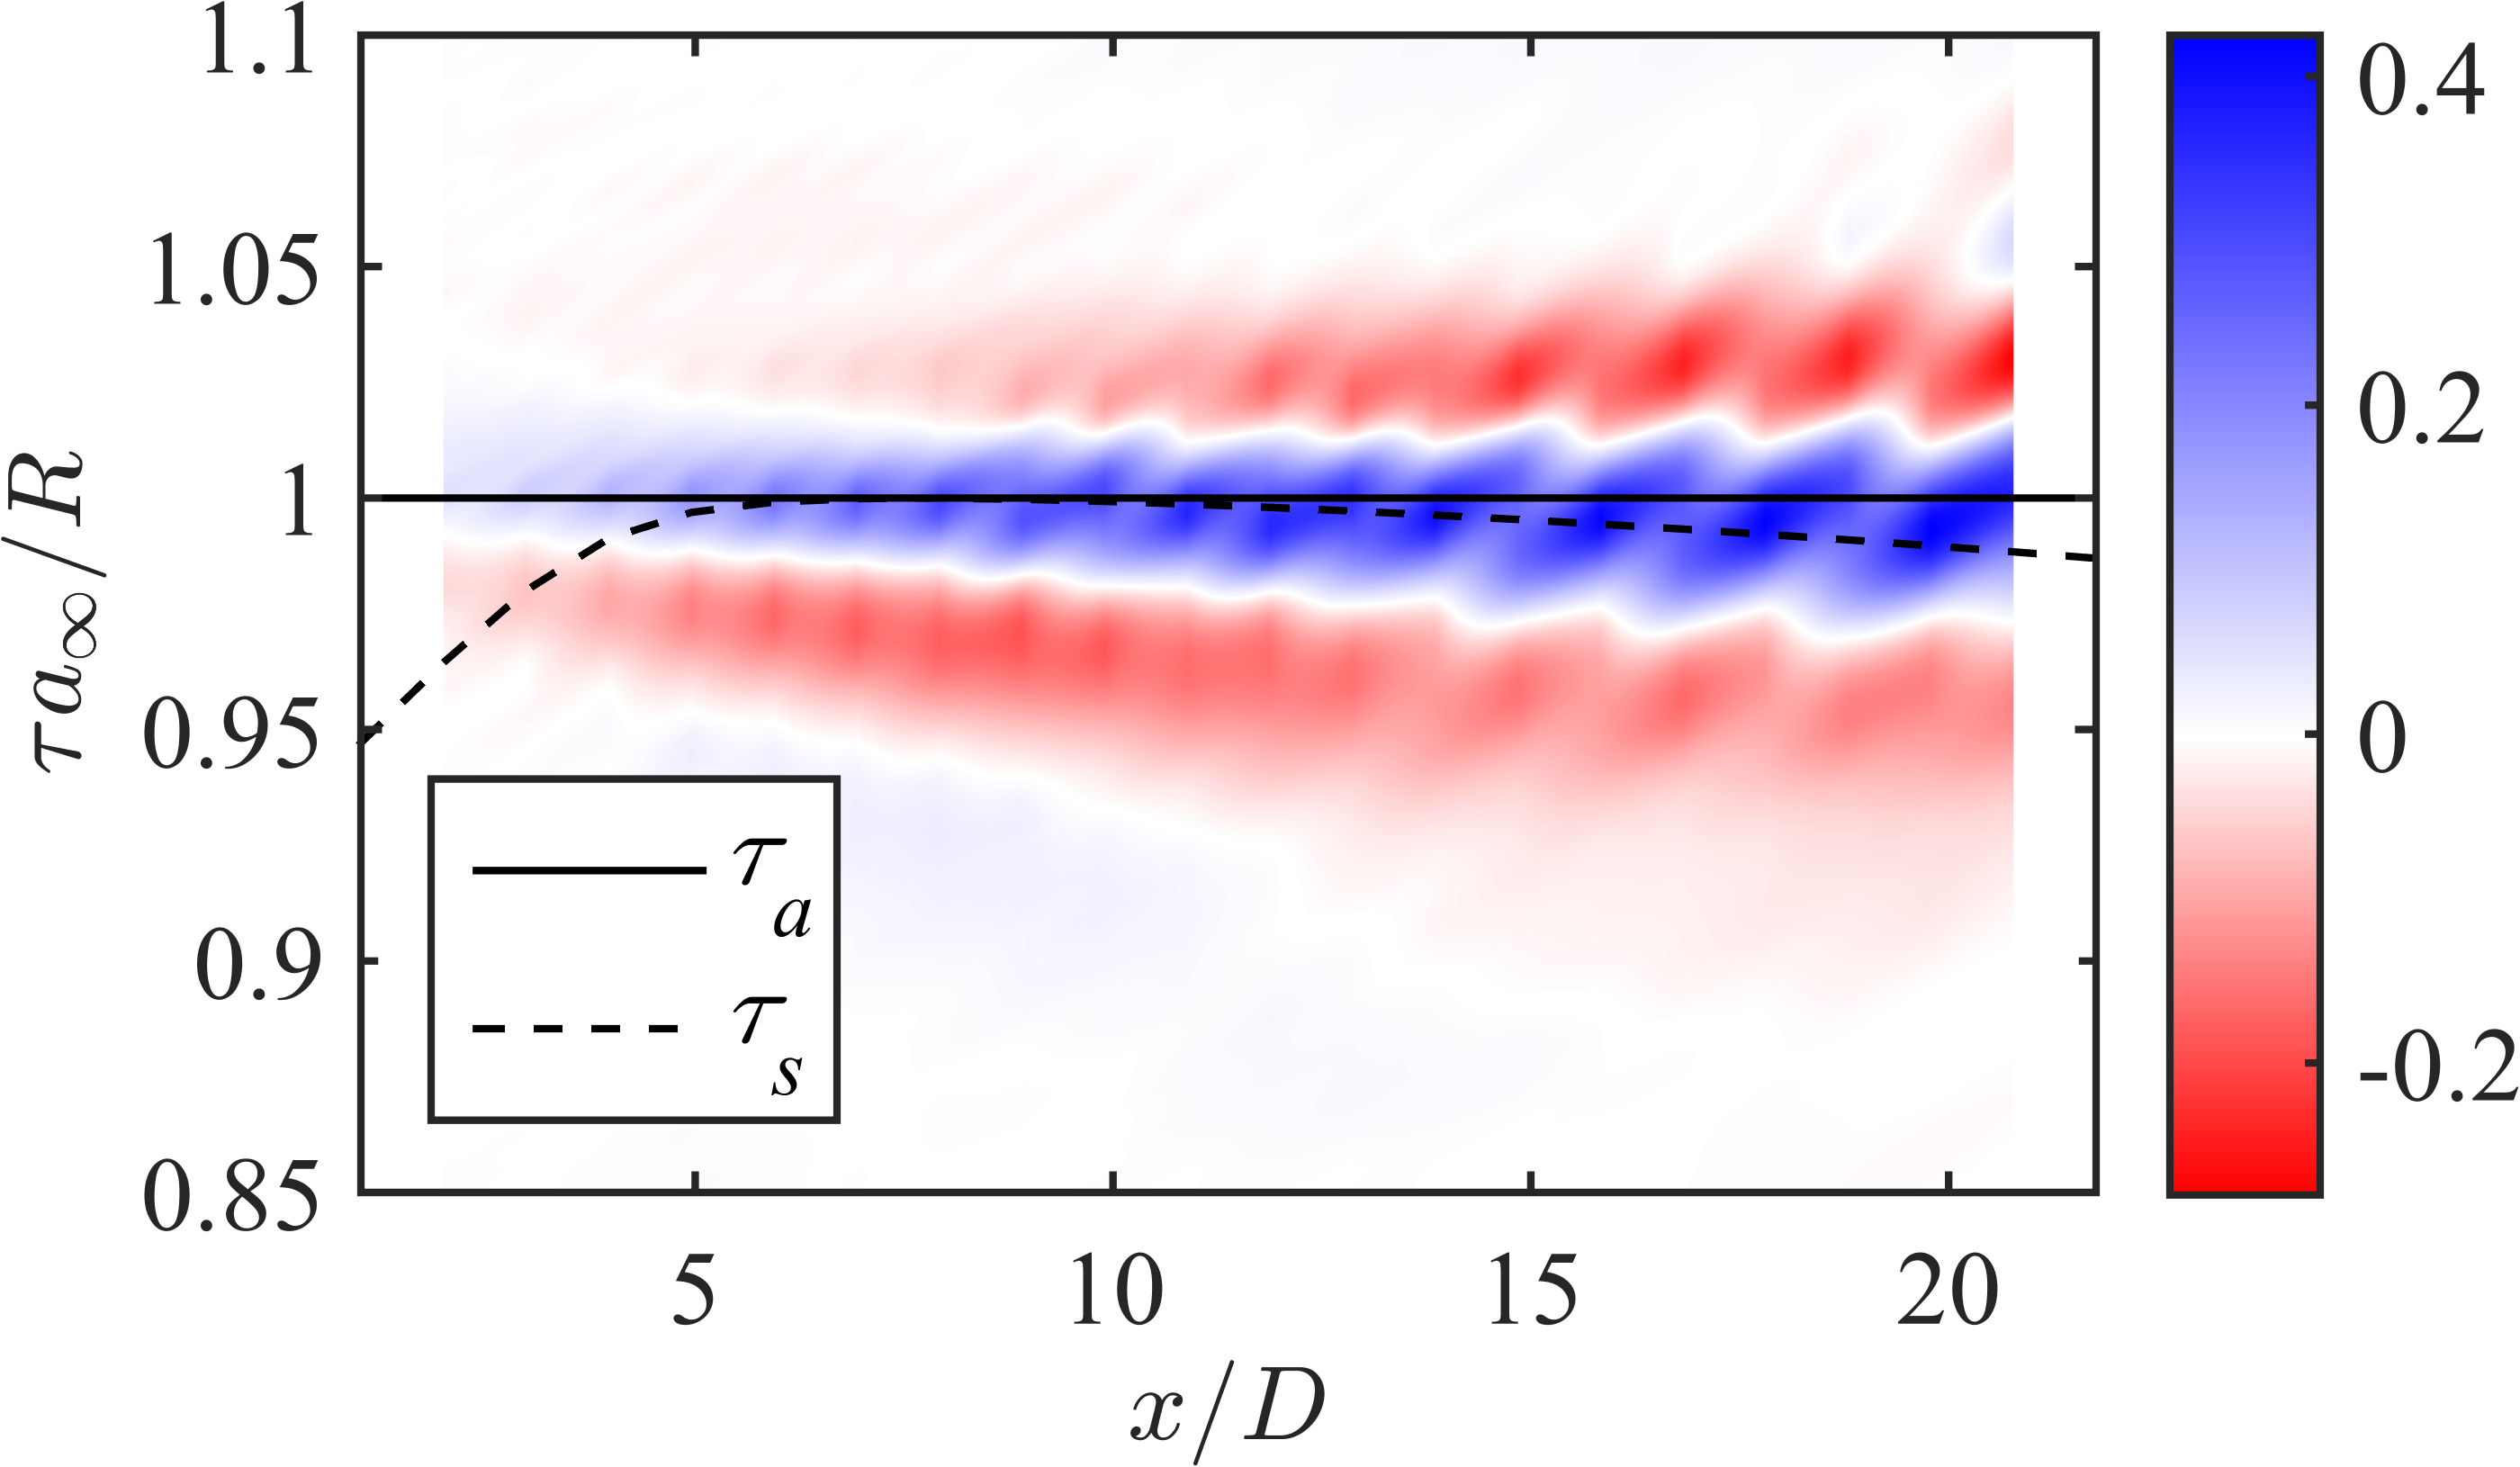
\includegraphics[width=0.95\linewidth]{Figures/St000_r120_ff30xcor_xcor_oa.png}
		\caption{}
		\label{fig:ch3_xcorrOA_St000}
	\end{subfigure}%
	\begin{subfigure}{.5\textwidth}
		\centering
		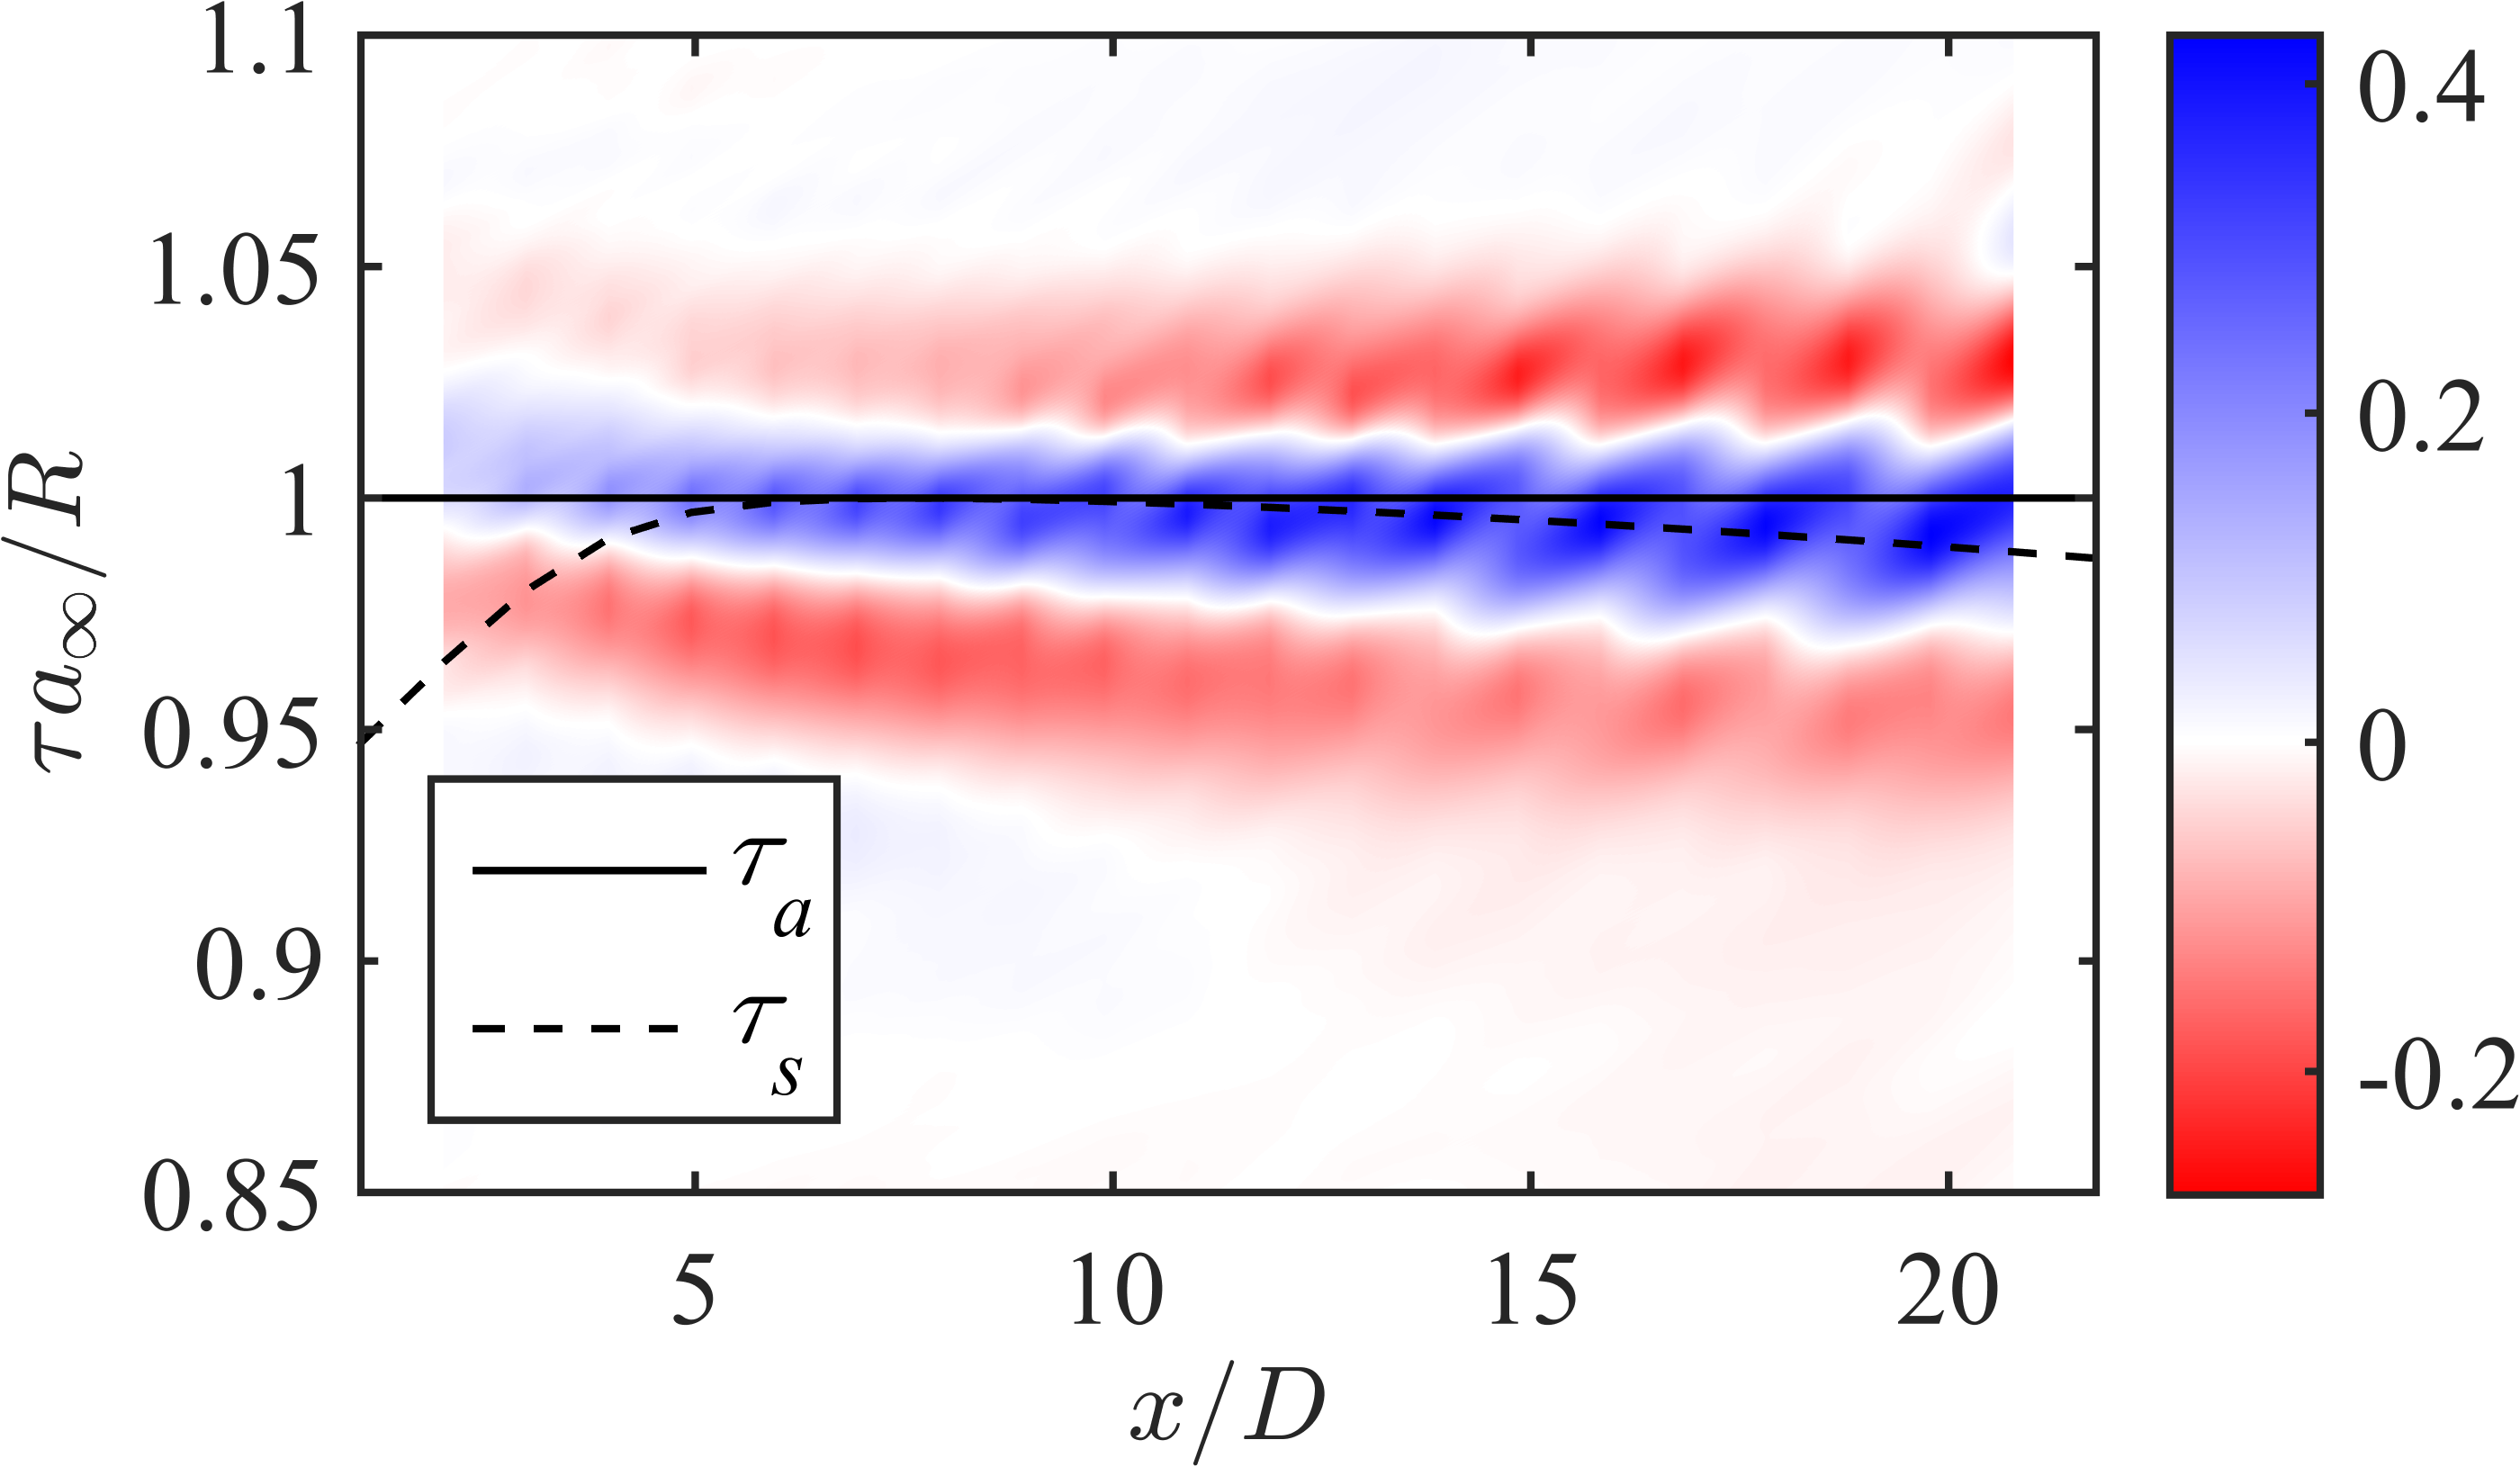
\includegraphics[width=0.95\linewidth]{Figures/St005_r120_ff30xcor_xcor_oa.png}
		\caption{}
		\label{fig:ch3_xcorrOA_St005}
	\end{subfigure}\\
	\begin{subfigure}{.5\textwidth}
		\centering
		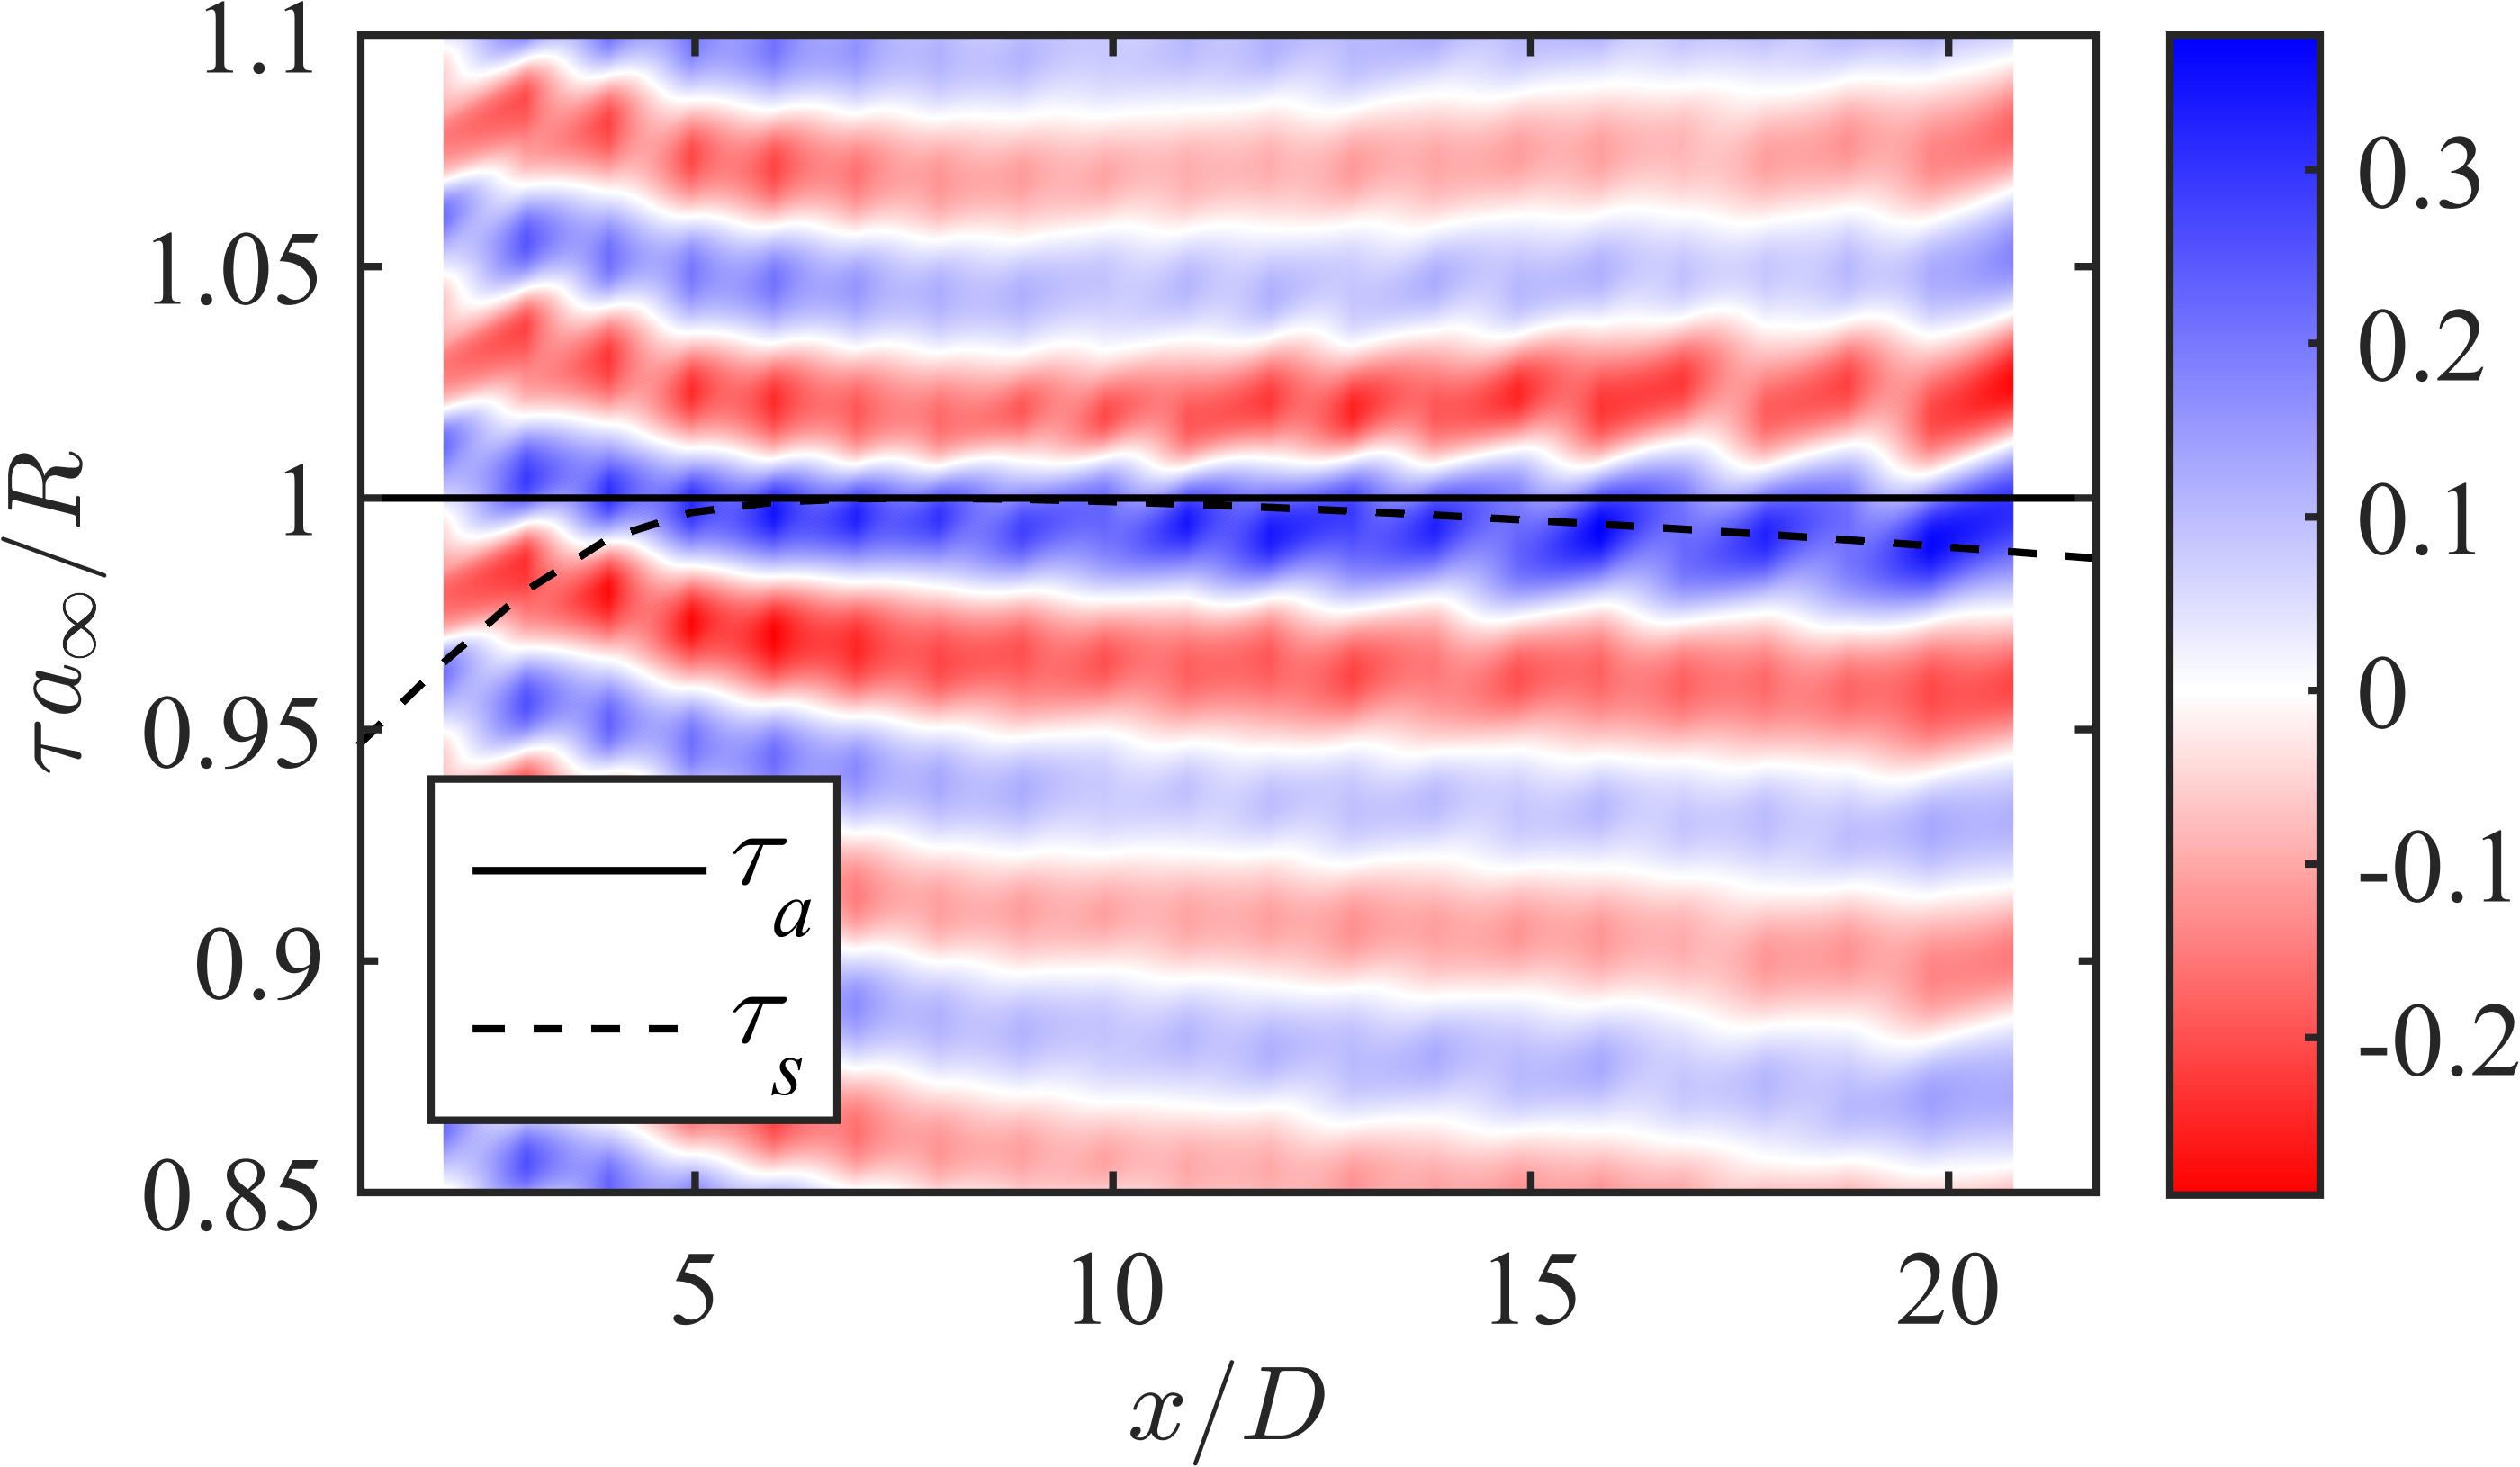
\includegraphics[width=0.95\linewidth]{Figures/St025_r120_ff30xcor_xcor_oa.png}
		\caption{}
		\label{fig:ch3_xcorrOA_St025}
	\end{subfigure}%
	\begin{subfigure}{.5\textwidth}
		\centering
		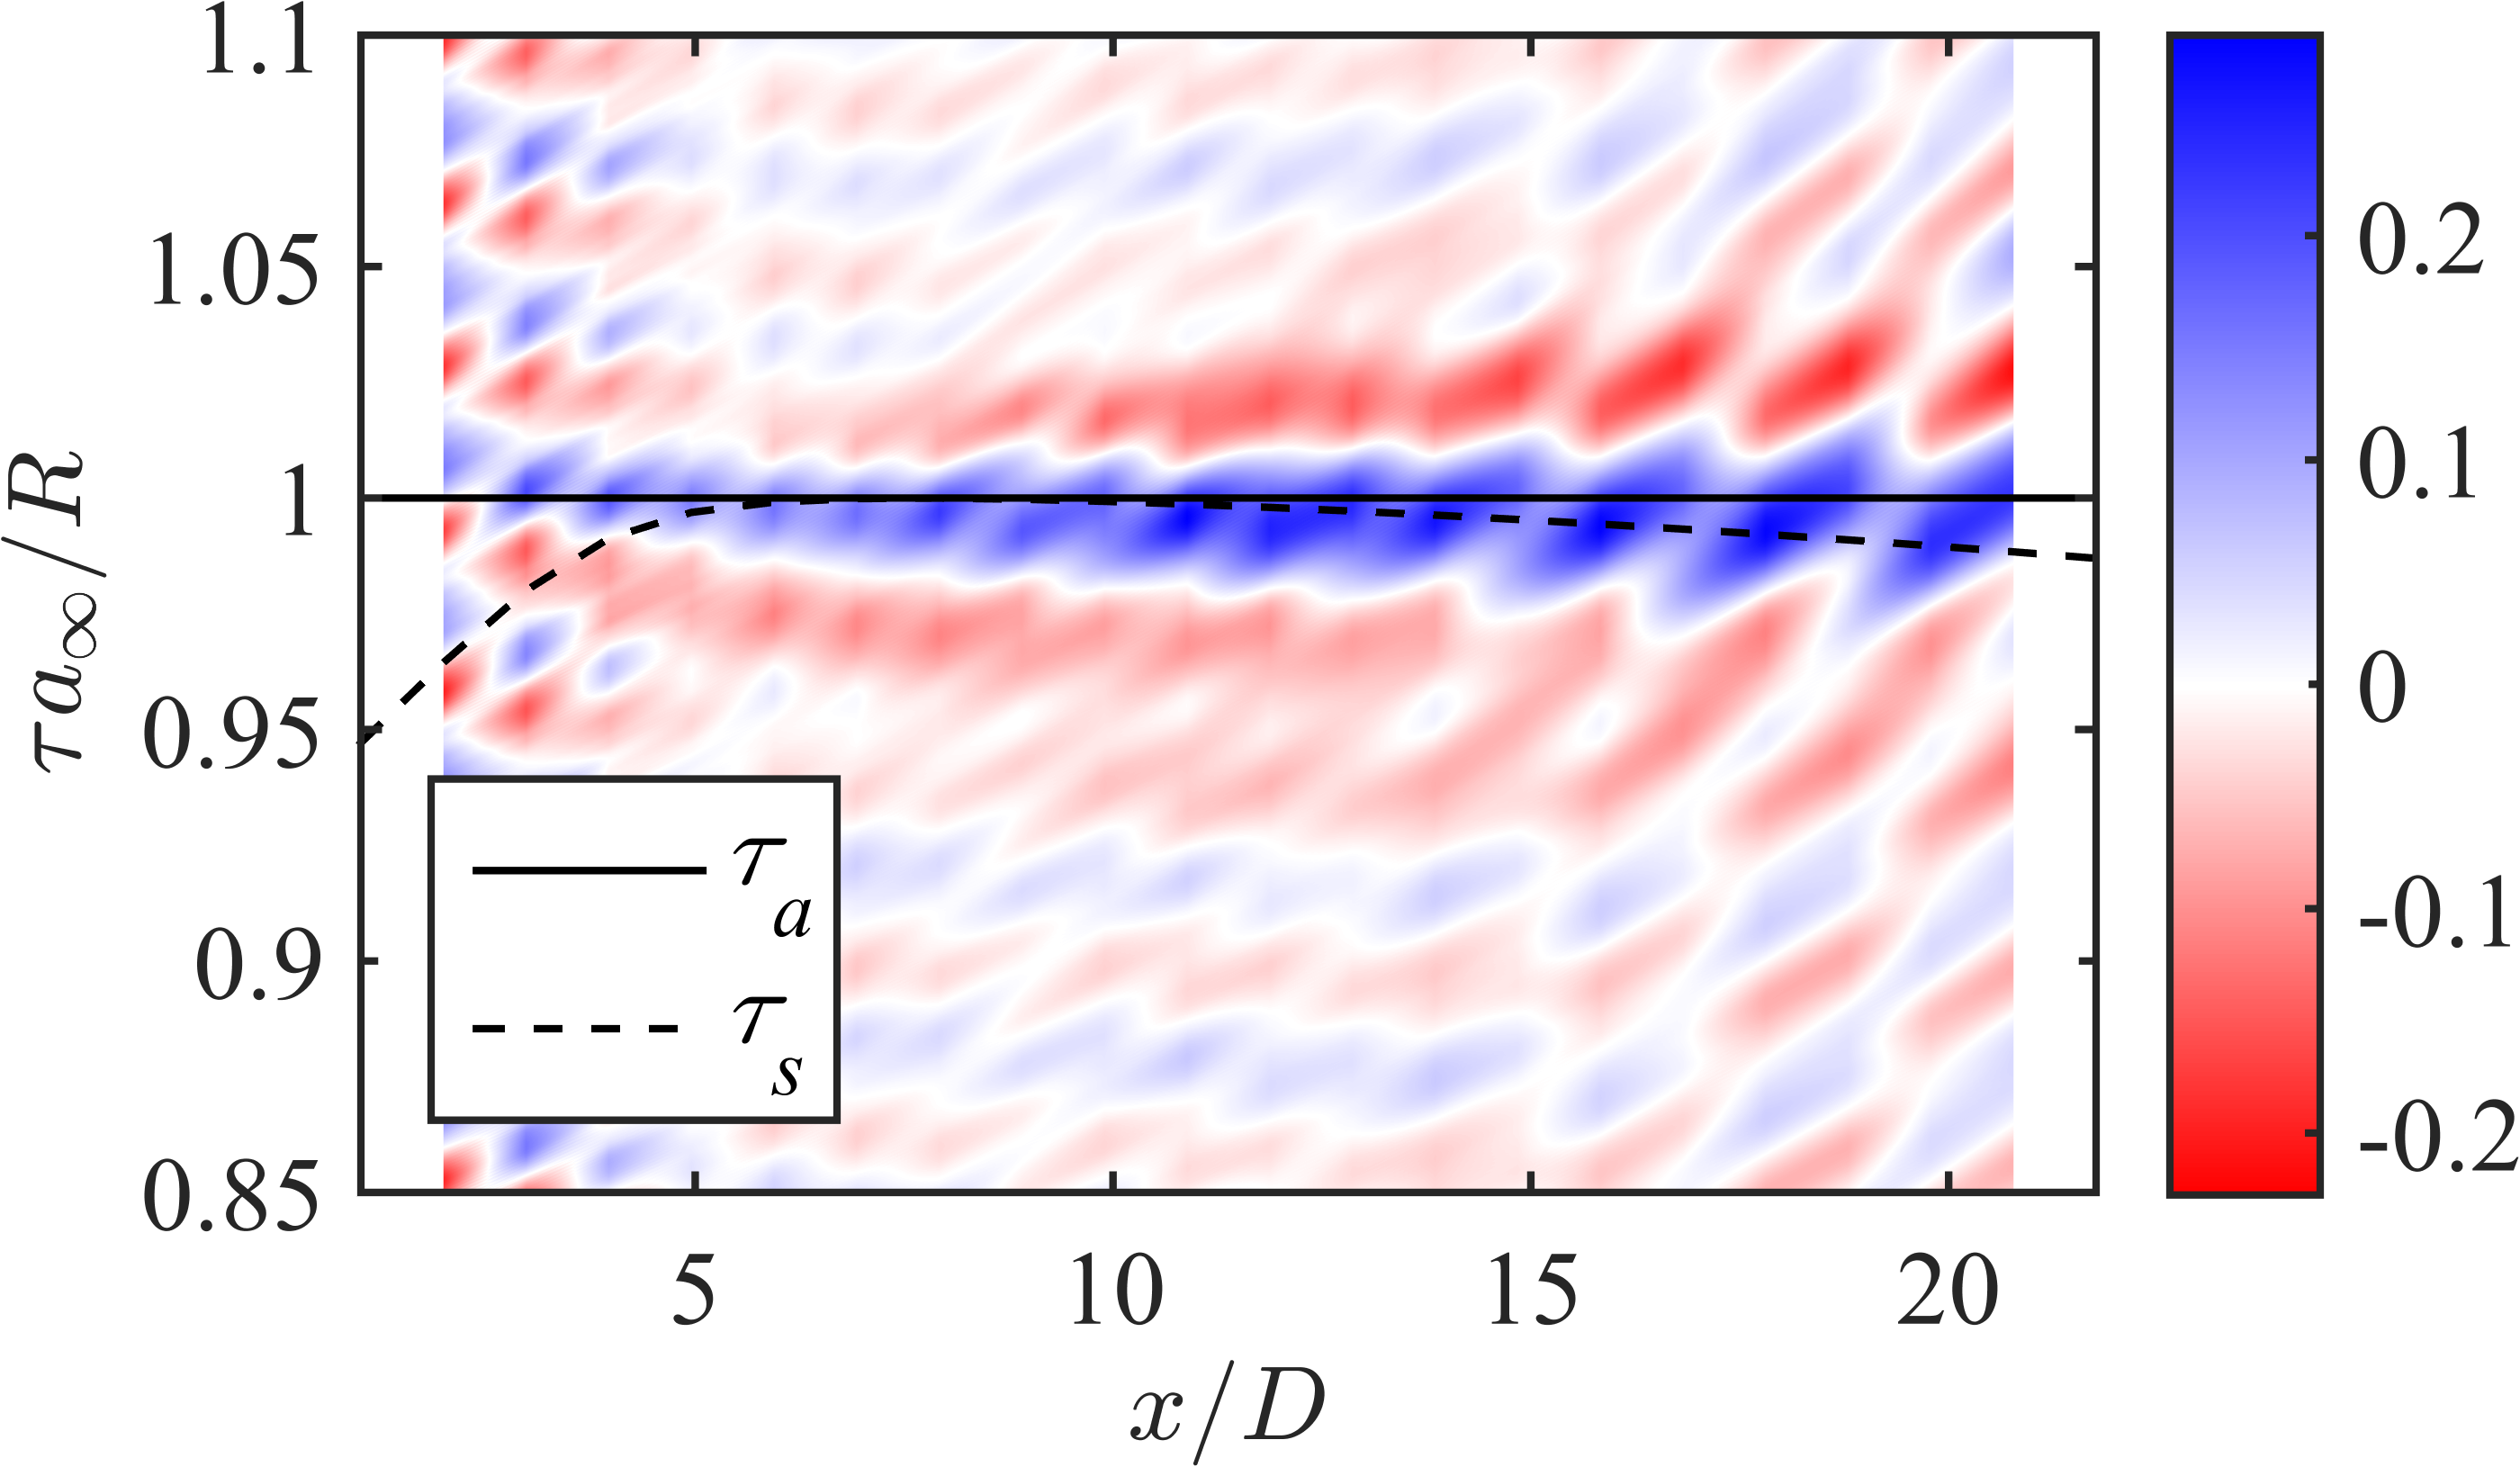
\includegraphics[width=0.95\linewidth]{Figures/St035_r120_ff30xcor_xcor_oa.png}
		\caption{}
		\label{fig:ch3_xcorrOA_St035}
	\end{subfigure}
	\caption{Normalized two-point correlations between the acoustic component of the near field and the far field at $30^\circ$ for microphone array position starting at $x/D = 1, r/D = 1.2$ for the natural jet (a), $St_{DF} = 0.05$ (b), $St_{DF} = 0.25$ (c) and $St_{DF} = 0.35$ (d).}
	\label{fig:ch3_xcorrOA}
\end{figure}

However, these results should not be interpreted as indicating that the source mechanisms are necessarily consistent for all excitation frequencies. 
For the lower-frequency periodic excitation ($St_{DF} \leq 0.25$), the consistency in the far-field response (\fig{fig:ch3_farfield_linear}) coupled with the consistency in the apparent source region is suggestive of a consistent dominant source mechanism.
In contrast, the inconsistency in the far-field response for the higher-frequency periodic excitation ($St_{DF} \geq 0.35$, \fig{fig:ch3_farfield_nonlinear}) is suggestive of a change in the dominant source mechanism, just one that is associated with the vortex dynamics in the jet shear layer upstream of the end of the potential core.
It should also be noted that the peak correlation values between the acoustic near-field and the far-field are significantly lower (though certainly non-negligible) in the periodic excitation cases, suggesting a decaying coherence in the source mechanisms at these frequencies.

The author would like to make a special note here, concerning the discrepancy between the results presented in \fig{fig:ch3_xcorrOA} and those presented previously in Crawley \etal \citep{Crawley2015}.
In that paper, the more simple Fourier filter was used to decompose the irrotational near-field; processing artifacts were noted and a parametric study was attempted to minimize their impact.
In the resulting two-point correlations of the decomposed acoustic field, a shift in the apparent source region was noted to coincide with the shift of the peak pressure fluctuations measured just outside the shear layer (higher frequency excitation cases saturating further upstream near the nozzle exit).
Because this behavior was observed across the entire range of filter parameters used, it was assumed to be representative of the true physical behavior and not a numerical artifact.
Of course, this assumption precludes the possibility that \textit{the entire parameter space produced similar numerical artifacts}. 

As discussed more thoroughly Crawley \& Samimy \citep{Crawley2016}, the Fourier filter had a tendancy to allow energy leakage from the hydrodynamic field into the acoustic, particularly at low frequencies. 
Since it has already been observed that the hydrodynamic signature of the large-scale structures can linearly correlate to the acoustic emission, a potential consequence of this leakage is correlation regions which instead point to the region of high hydrodynamic energy - i.e. the saturation point of the near-field pressure fluctuations.
There are few certainties in life beyond death and taxes, so it is difficult the argue with definitiveness that the results depicted in the present work are entirely free of numerical artifacts.
However, the analysis found in Crawley \& Samimy \citep{Crawley2016} demonstrate that wavelet filter is more robust in this regard, and as such the author is inclined to lend more credence to the results presented herein. 
From the current results alone, the significance of this estimated source region is not entirely clear.
In \sect{sect:velocity} the time-resolved velocity field will be explored in detail to better elucidate the structure dynamics, with a particular focus on the region just upstream of the end of the potential core.  
\chapter{Estimation of Time-resolved Velocity Fields}
\label{sect:velocity}
Analysis of the evolution, interaction, and disintegration of the large-scale structures, and ultimately the noise generated thereby, is greatly simplified by the acquisition of time-resolved flow-field measurements.
Furthermore, as will be explained in \sect{sect:source}, computation of the aeroacoustic source field from a simplified acoustic analogy will require time-resolved flow-field data.
Unfortunately, directly acquiring time-resolved velocity fields for the jet currently under study is simply not possible due to the combination of a large domain of interest ($0 \leq x/D \lesssim 12, 0 \leq r/D \lesssim 3$) and high characteristic frequencies on the order of several kHz.
Full-field, high-fidelity measurement techniques capable of this required repetition rate simply do not exist at present.
An indirect method is therefore required in order to estimate the evolution of the large-scale structures, in a reduced-order sense.

Phase-locking of a data acquisition system to a reference signal (such as an actuator or a naturally occurring resonance tone) is a common experimental technique; by varying the delay between the trigger and time of data acquisition, multiple phases can be acquired and the coherent component of the phenomena can be analyzed.
Phase-locking of the PIV system to the LAFPAs was initially considered for the present work, but quickly discarded.
Sample analysis performed using a numerical database indicated that a very high temporal resolution was required in order to accurately compute fluctuation rates in the dilatation field (the relevance of which will become more apparent in the following chapter).
At moderate to high excitation frequencies, this was feasible, though potentially tedious (for example, $\sim$16 phases were estimated as necessary at $St_{DF} =0.25$).
At $St_{DF} =0.05$ however, this would require roughly \textit{forty} phases (the significant dead time between actuations means that it is not necessary to acquire the entire range of phases from $0$ to $2\pi$, but this is small consolation).
Clearly, a more efficient data acquisition method is needed.
\section{Stochastic Estimation}
Stochastic estimation was first proposed by Adrian \citep{Adrian1977} in 1977, as a methodological formalization of the conditional statistical analyses popular at the time. 
Large-scale coherent structures had been educed from anisotropic turbulent flows (such as boundary or shear layers) by conditional sampling techniques.
Adrian succeeded in identifying detailed flow structures (`conditional eddies') in isotropic turbulence by computing a mean-square estimate of the flow from linear two-point correlations (higher-order, nonlinear correlations were explored in Adrian \citep{Adrian1979}). 
The methodology was extended in Adrian \citep{Adrian1994} to estimation of velocity fields using spatial correlations coupled with a reduced set of measurements.

Stochastic estimation attracted considerable attention from the fluid dynamics community due to its potential to educe meaningful structures and behavior from highly turbulent, incoherent flows as well as its relative simplicity.
Subsequent researchers refined stochastic estimation in several important aspects.
Bonnet \etal \citep{Bonnet1994} developed the complementary technique by combining linear stochastic estimation (LSE) with proper orthogonal decomposition (POD), improving the accuracy due to higher correlation levels between low-order modes.
The estimated velocity fields produced by LSE were projected onto the POD eigenfunctions (computed from the random, non-time-resolved velocity fields) to produce an estimate of the time-dependent POD coefficients, which can then be used to reconstruct low-order representations of the estimated random velocity field.
Picard \& Delville \citep{Picard2000} used LSE and POD to link the longitudinal pressure distribution surrounding a low subsonic jet to vortical motions in the shear layer by simultaneously sampling microphone and hotwire data.
In Boree \citep{Boree2003} the POD coefficients of the velocity field were estimated directly, using pressure modes.
Ewing \& Citriniti \citep{Ewing1997} extended the standard form of LSE, in which spatial correlations are computed at a single time lag, by Fourier transforming the reference signal in time prior to computing the two-point cross-correlations (now cross-spectra). 
The incorporation of phase-delay information over a range of frequencies (and in essence, including information from multiple time lags) was found to significantly improve the accuracy of the reconstructions for many flow regimes \citep{Ewing1997,Tinney2006,Tinney2008b}.
Finally, multi-time-delay LSE-POD was performed in the physical domain (as opposed to the Fourier) by Durgesh \& Naugton \citep{Durgesh2010} to study the turbulent structures in a near wake region.

The current work borrows heavily from the methodology of Tinney \etal \citep{Tinney2008b} and Sinha \etal \citep{Sinha2010} in order to estimate the two-component time-resolved velocity field on a streamwise slice of the jet.
As explained in \sect{sect:piv_method}, two-component PIV snapshots were acquired at well-defined instants of experimentally recorded near-field pressure traces.
The computational methodology by which the stochastic estimation is performed has been modified, however.
Complementary stochastic estimation is used, due to its significantly lower computational cost as well as theorized improvement in accuracy.
Thus, the instantaneous velocity fields will be separated into characteristic modes via POD and the time-dependent modal coefficients, rather than the velocity fields themselves, will be estimated using SE.
Instead of performing the stochastic estimation using either linear or higher-order cross-correlations (or cross-spectra), the conditional mapping between the near-field pressure and the POD modal coefficients will be generated by an artificial neural network with multi-time-delay.
Artificial neural networks were chosen over the more traditional cross-correlations due to their simplicity compared to high-order methods as well as their demonstrated ability to model nonlinear processes in turbulent flows \citep{Lasagna2015}.

\subsection{Stochastic Estimation via Artificial Neural Networks}
Artificial neural networks (ANNs), are statistical computing models which developed as a branch of machine learning.
The design of neural networks is based on simplified models of the human brain: they are comprised of a large number of simple, interconnected computing cells (`neurons') and therefore are massively parallel distributed processors.
The neurons themselves are based on models of biological neurons, and produce a single output based on the linear summations of inputs (either directly from the user or from other, lower-level neurons) and synaptic weights which is then modulated by a nonlinear activation function.
The synaptic weights are modified by a learning algorithm in order to minimize a cost function; this generally takes the form of explicit training (supervised learning).
The interconnectivity of a massive number of these nonlinear computing cells allows artificial neural networks to approximate unknown, nonlinear functions of an arbitrary number of inputs while retaining a certain, elegant, simplicity.
It should be unsurprising then, that ANNs have already been applied for the estimation and control of a variety of turbulent flow regimes.
Interested readers are recommended to refer to Haykin \citep{Haykin1994} for an extensive background on artificial neural networks, their developmental history, and many additional network structures not used in this work.

A feedforward network structure was used in the current work, a schematic of which can be found in \fig{fig:ch4_neural_net}.
The ANN was comprised of an input layer, to which near-field pressure traces were supplied, a single hidden layer containing 32 neurons, and an output layer which produced estimates of the time-varying POD coefficients. 
The hidden and output layers were fully connected, and the modified logistic function (hyperbolic tangent) was used as the activation function.
The pressure traces were centered around the acquisition of a PIV image group, and was downsampled to 200 kHz in order to approximate the frequency response of the microphones.
The record time supplied for each training block was $\pm 2.56$ milliseconds; this was determined by estimating the time delay for a large-scale structure to convect through the experimental domain (the convective velocity of the large-scale structures was conservatively estimated as $U_c \simeq 0.5 U_j$).
A visual representation of this process has been supplied in \fig{fig:ch4_pressure_mapping}, where sample pressure traces from the near-field microphone array, centered around an instantaneous velocity snapshot, are shown.
For ease of understanding, the fluctuating component of the velocity field is shown here; in practice the neural network was used to predict the time-dependent POD expansion coefficients which were then used to reconstruct the velocity fluctuations.
\begin{figure}
	\centering
	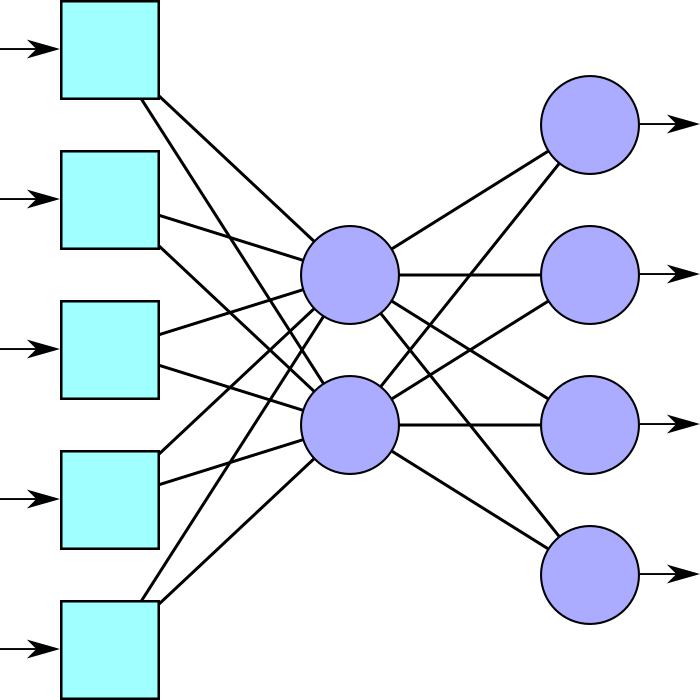
\includegraphics[width = 2in]{Figures/neural_net_v2.png}
	\caption{Schematic of a feedforward ANN with a single hidden layer. The activation function is applied only to the hidden and output layers. The number of neurons depicted in each layer is meant to represent the \textit{relative} number used by the actual ANN.}
	\label{fig:ch4_neural_net}
\end{figure} 

\begin{figure}
	\centering
	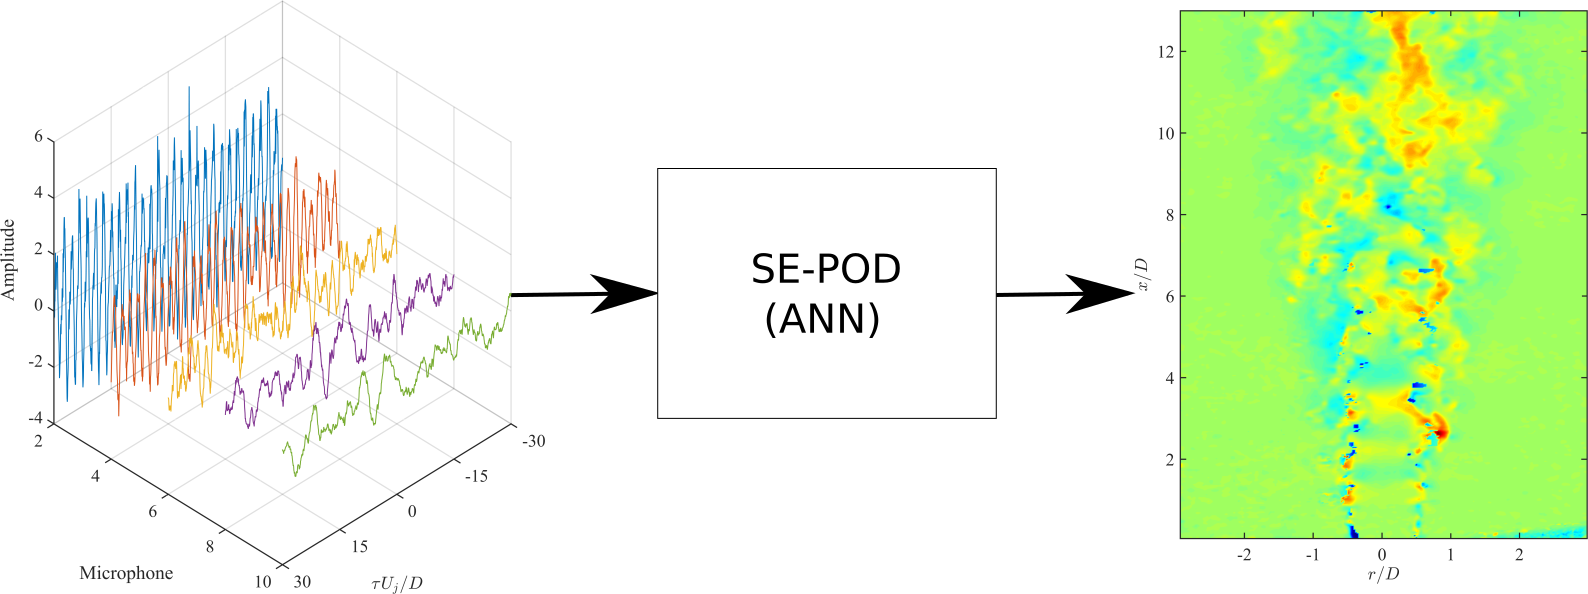
\includegraphics[width = \linewidth]{Figures/pressure_mapping.png}
	\caption{Schematic showing sample pressure traces from the irrotational near-field which are supplied to the neural network in order to train it to predict the fluctuating component of the velocity instantaneous velocity.}
	\label{fig:ch4_pressure_mapping}
\end{figure}

POD modes and time-varying coefficients were computed from the velocity fields using the method of snapshots \citep{Sirovich1987}; the kernel was defined as the two-component turbulent kinetic energy.
The instantaneous velocity fields were not preprocessed prior to the decomposition (that is, missing or spurious vectors were not replaced or interpolated).
As experimental noise in the velocity fields will be completely uncorrelated to the near-field measurements, it will be filtered out by the stochastic estimation and hence preprocessing is unnecessary.
In this work, the coefficients for every POD mode were estimated, rather than just the most energetic modes, for two reasons.
First, it is not guaranteed that an individual POD mode corresponds to a physically distinct turbulent flow structure or event - an event may be broken up into multiple POD modes of varying energy levels.
Secondly, the most energetic POD mode is not necessarily the most relevant mode for the acoustic generation process (see Jordan \etal \citep{Jordan2007} for a modification to the standard POD kernel in order to mitigate this issue).
The second issue is in fact not unique to the field of aeroacoustics but vexes turbulence research in general, where highly relevant dynamical processes may contain little energy \citep{Noack2008}; this has lead researchers to propose alternative methods for extracting dynamical features of turbulent flows \citep{Schmid2010}.

Even though the network is estimating even the least-energetic modes, the current method is far more computationally efficient than directly estimating the velocity fields themselves.
By encoding spatial correlations in the POD expansion coefficients, estimation of the $N$ snapshots of $M \times K$ spatial locations has been reduced from a minimization problem of $N$ vectors of $2MK$ to one of $N$ vectors of $N$.
For the current experimental database, this means the system has been reduced from $290,508 \times 1500$ to $1500 \times 1500$.
The neural network now only needs to identify the temporal correlations between the pressure field and the individual POD coefficients; it does not need to learn the spatial correlations.

Learning was accomplished via the standard backpropagation method \citep{Haykin1994}, which approximates the error surface of the cost function using first-order derivatives; the error `propagates' backwards from the output neurons to the hidden neurons and the synaptic weights at each neuron are updated to identify the (hopefully, global) minimum of the cost function using gradient descent.
The cost function was defined as the mean-squared-error between the predicted and measured expansion coefficients for a given PIV image group.
The velocity field, $\mathbf{U}$ at a given instance, $k$, can be recovered from $N$ orthonormal modes, $\phi$, and time-varying expansion coefficients, $a_k$, as $\mathbf{U} = \sum_{n=0}^{N} a_{k}^{n} \phi^n$ \citep{Berkooz1993}.
The total energy of each mode is therefore encoded in $a_k^n$, which will serve as a simple energy weighting for the cost function (the importance of relative errors to the cost function will essentially be scaled by the energy in each particular mode).
Training of the network was performed using the roughly 1500 ensemble pressure-velocity blocks of data (a few PIV images in each set had to be discarded due to laser misfires); synaptic weights were updated based on the average of all blocks (batch processing) using a constant learning rate.
A well-known issue with the gradient descent optimization method is that it has a tendency to get trapped in local minima and fails to converge to the global minimum.
Therefore, sample results were also calculated using a much different learning algorithm: adaptive particle swarm optimization.
Details will not be presented here however, as the results were found to not differ substantially from those produced by the backpropagation algorithm (while requiring significantly higher computational resources).

\subsection{Reduced-Order Representation of the Flow-Field}
Ultimately, due to limitations both in the methodology as well as in the ability of the microphones located outside the flow to sense fine-scale turbulent fluctuations, the estimated velocity field is going to represent a reduced-order model of the jet.
This can be easily observed in \fig{fig:ch4_SEPOD_filtering}, where the measured axial fluctuating velocity field at an arbitrary instance in time has been plotted against the fluctuating velocity field produced by the SE-POD estimation from the near-field pressure at the same instance in time.
For comparison purposes, a reduced-order reconstruction of the measured velocity fluctuations from the first 100 POD modes (but without estimating from the near-field pressure using SE) has also been included.
Note that here the output of the model produced by SE-POD is being compared against a known output that the system is meant to match; this is not an evaluation of the \textit{predictive} power of the model but of the \textit{representative} power.
\begin{figure}
	\centering
	\begin{subfigure}{0.75\textwidth}
		\centering
		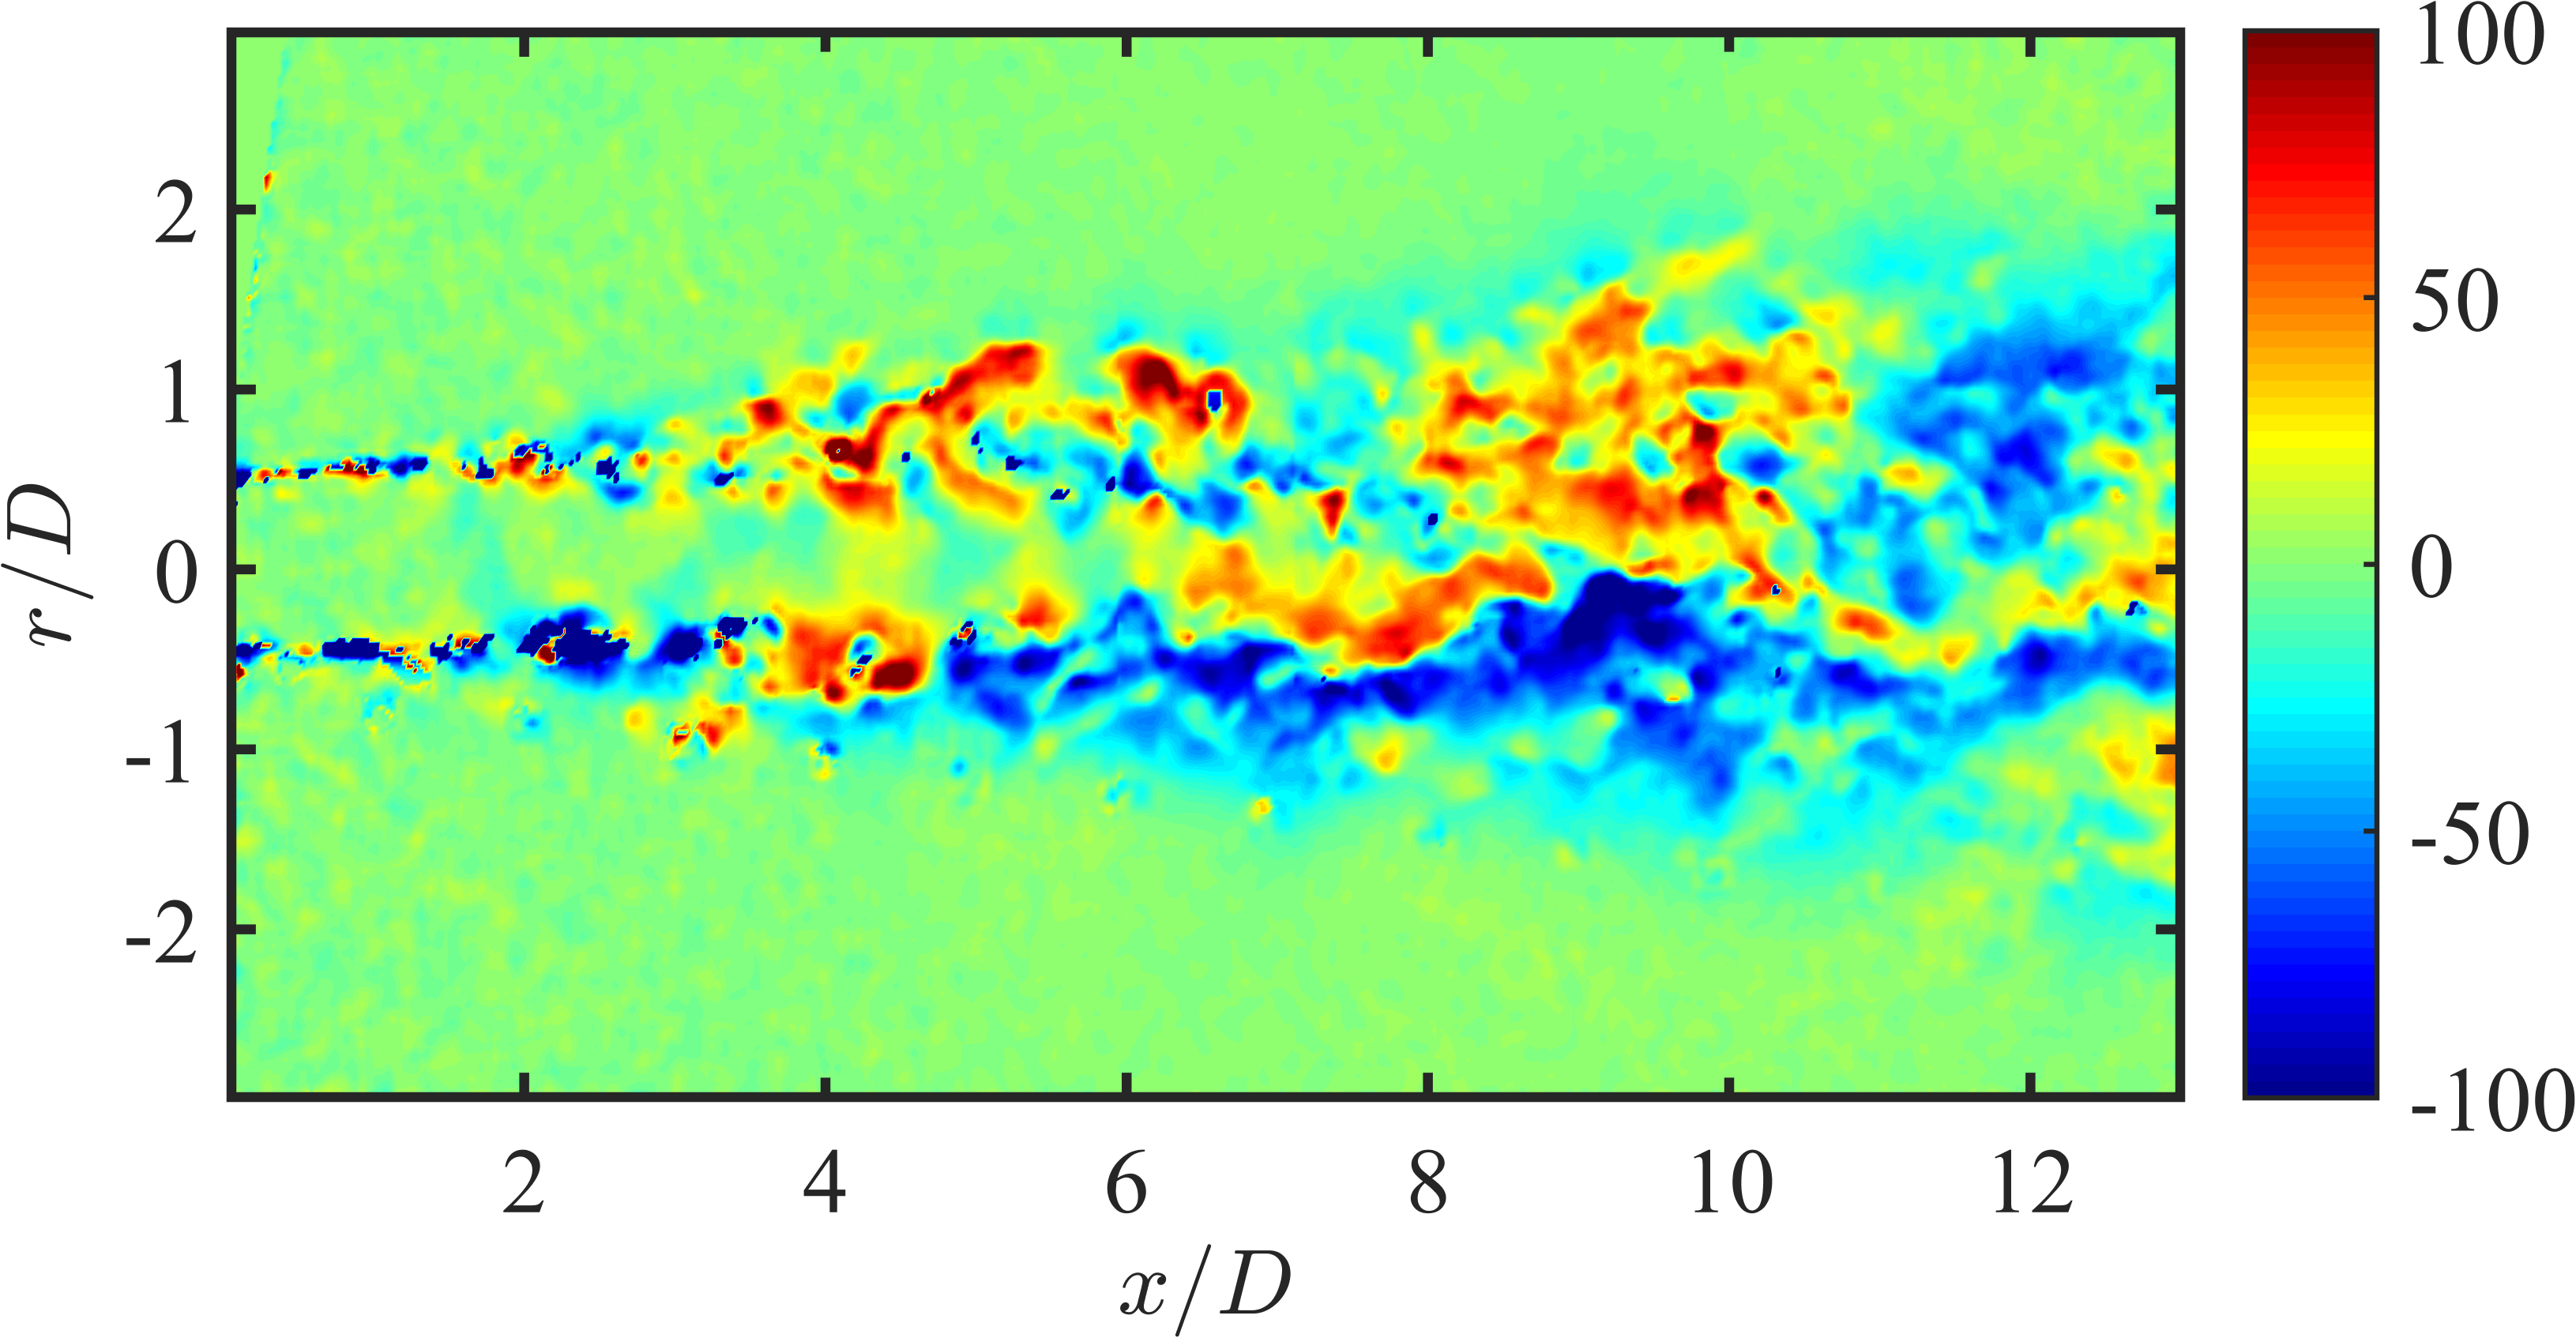
\includegraphics[width=0.95\linewidth]{Figures/ch4_Ux_true_v2.png}
		\caption{Measured}
	\end{subfigure}\\
	\begin{subfigure}{0.75\textwidth}
		\centering
		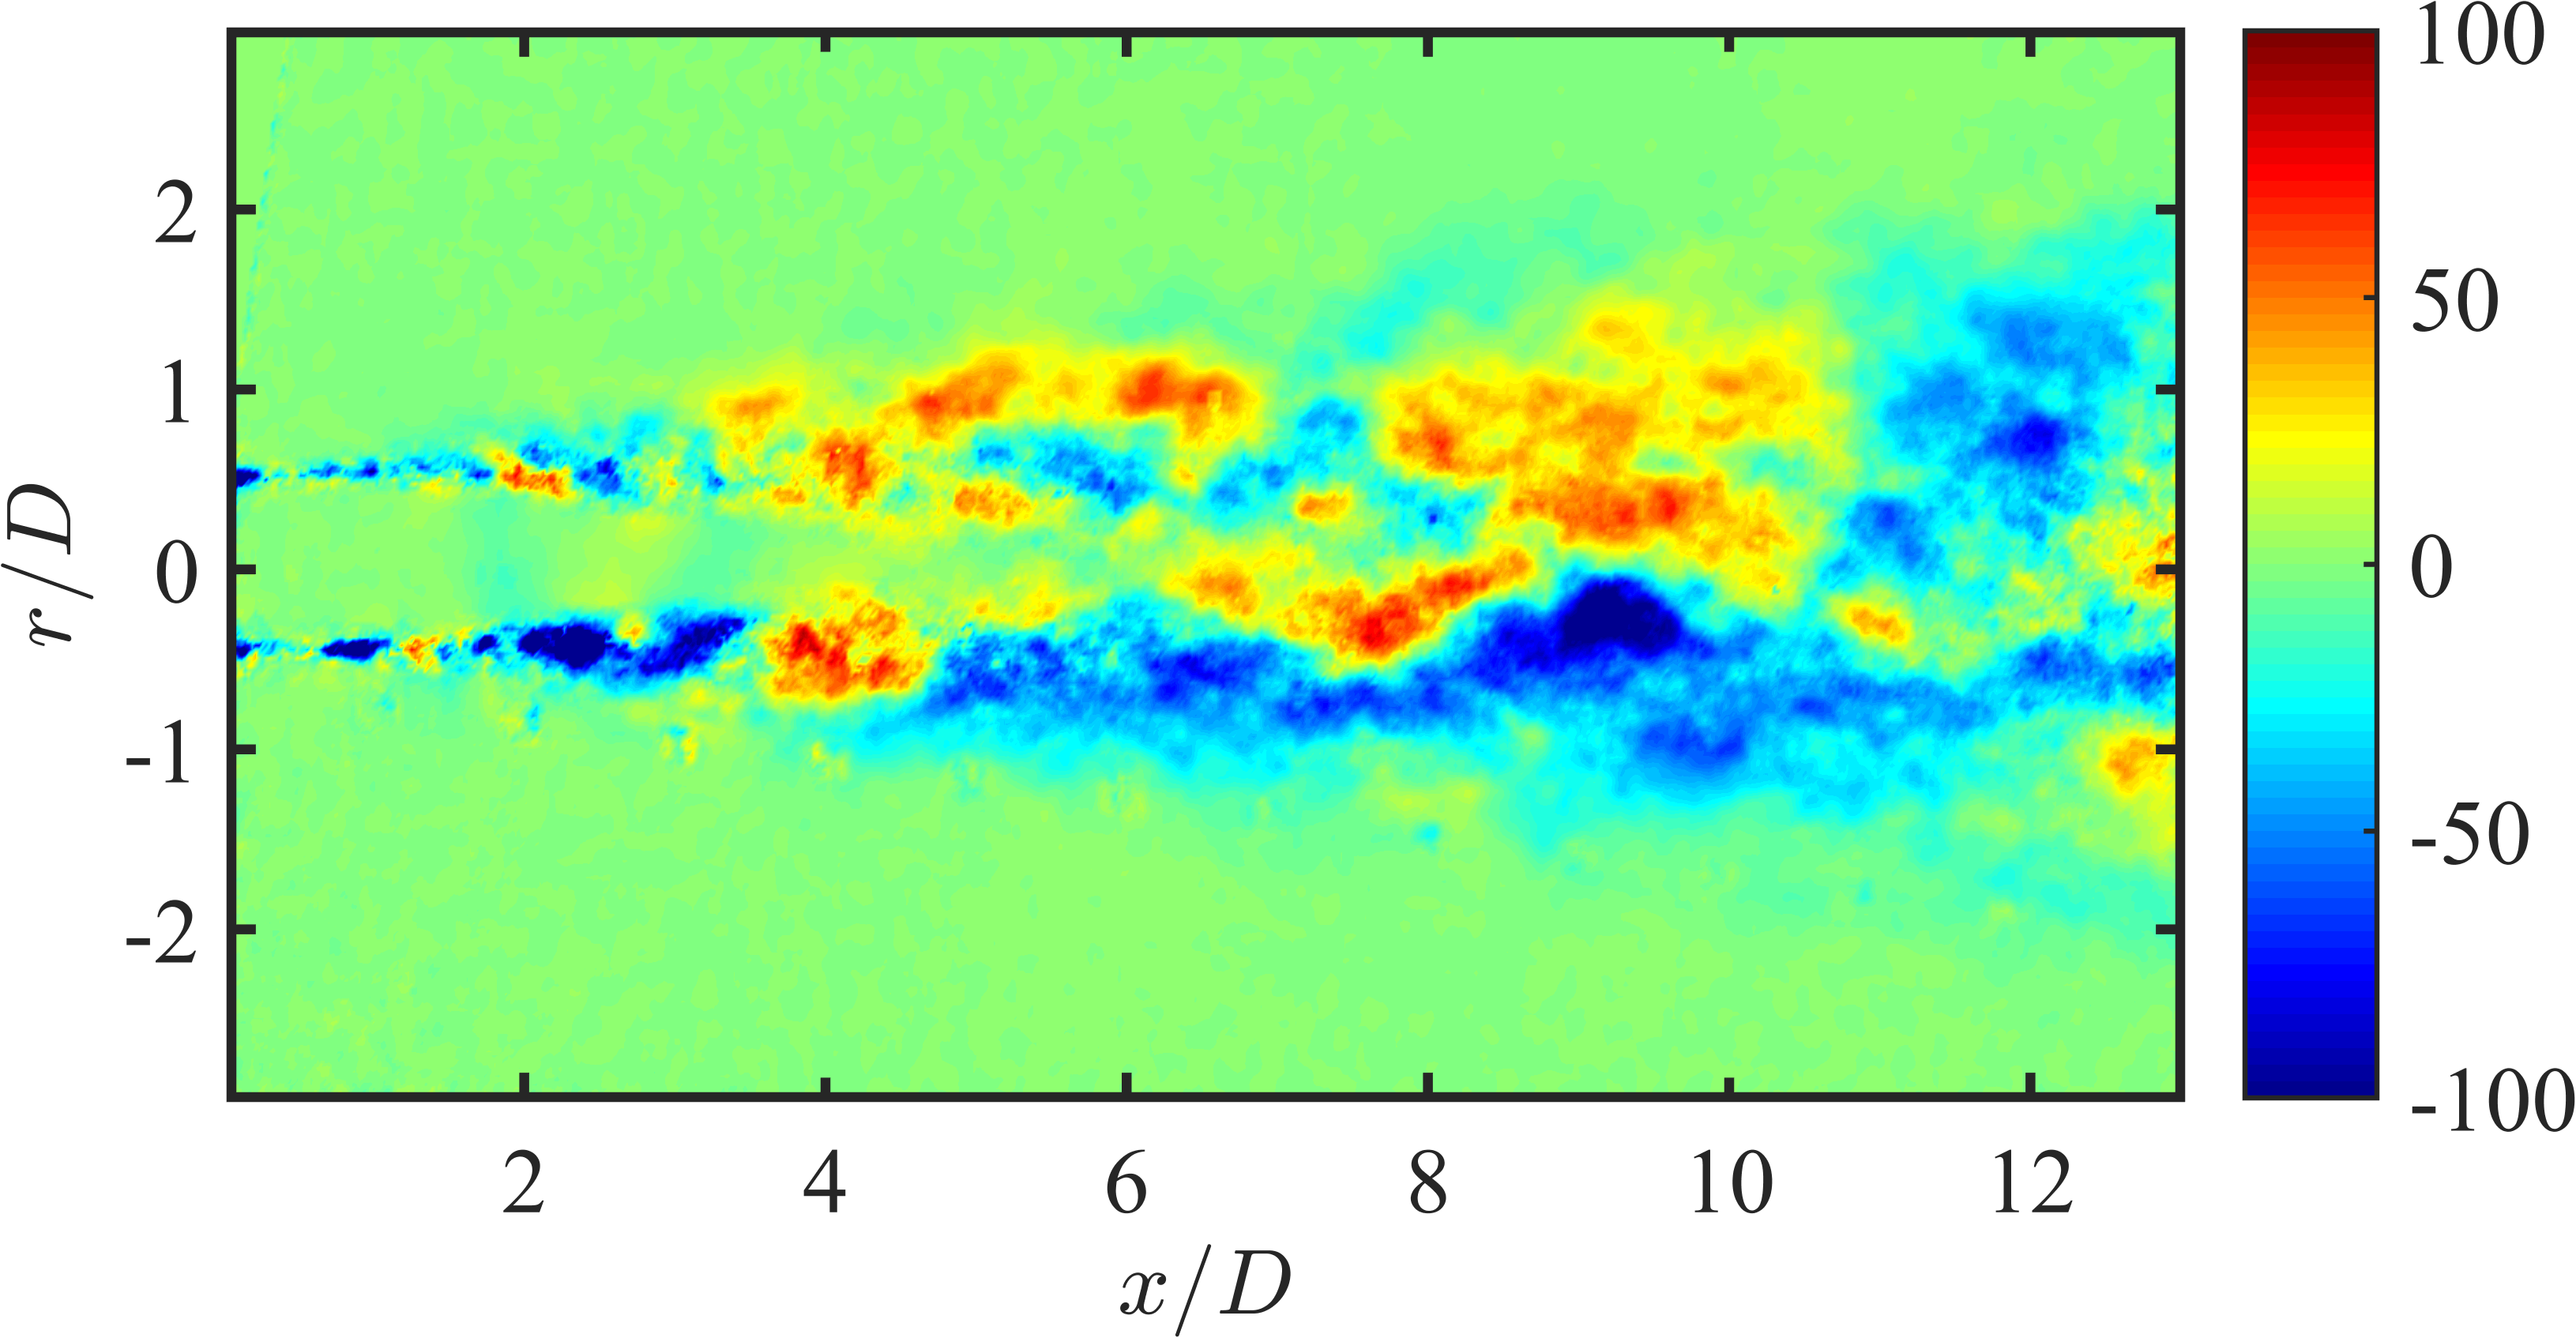
\includegraphics[width=0.95\linewidth]{Figures/ch4_Ux_estimated_v2.png}
		\caption{Estimated}
	\end{subfigure}
	\begin{subfigure}{0.75\textwidth}
		\centering
		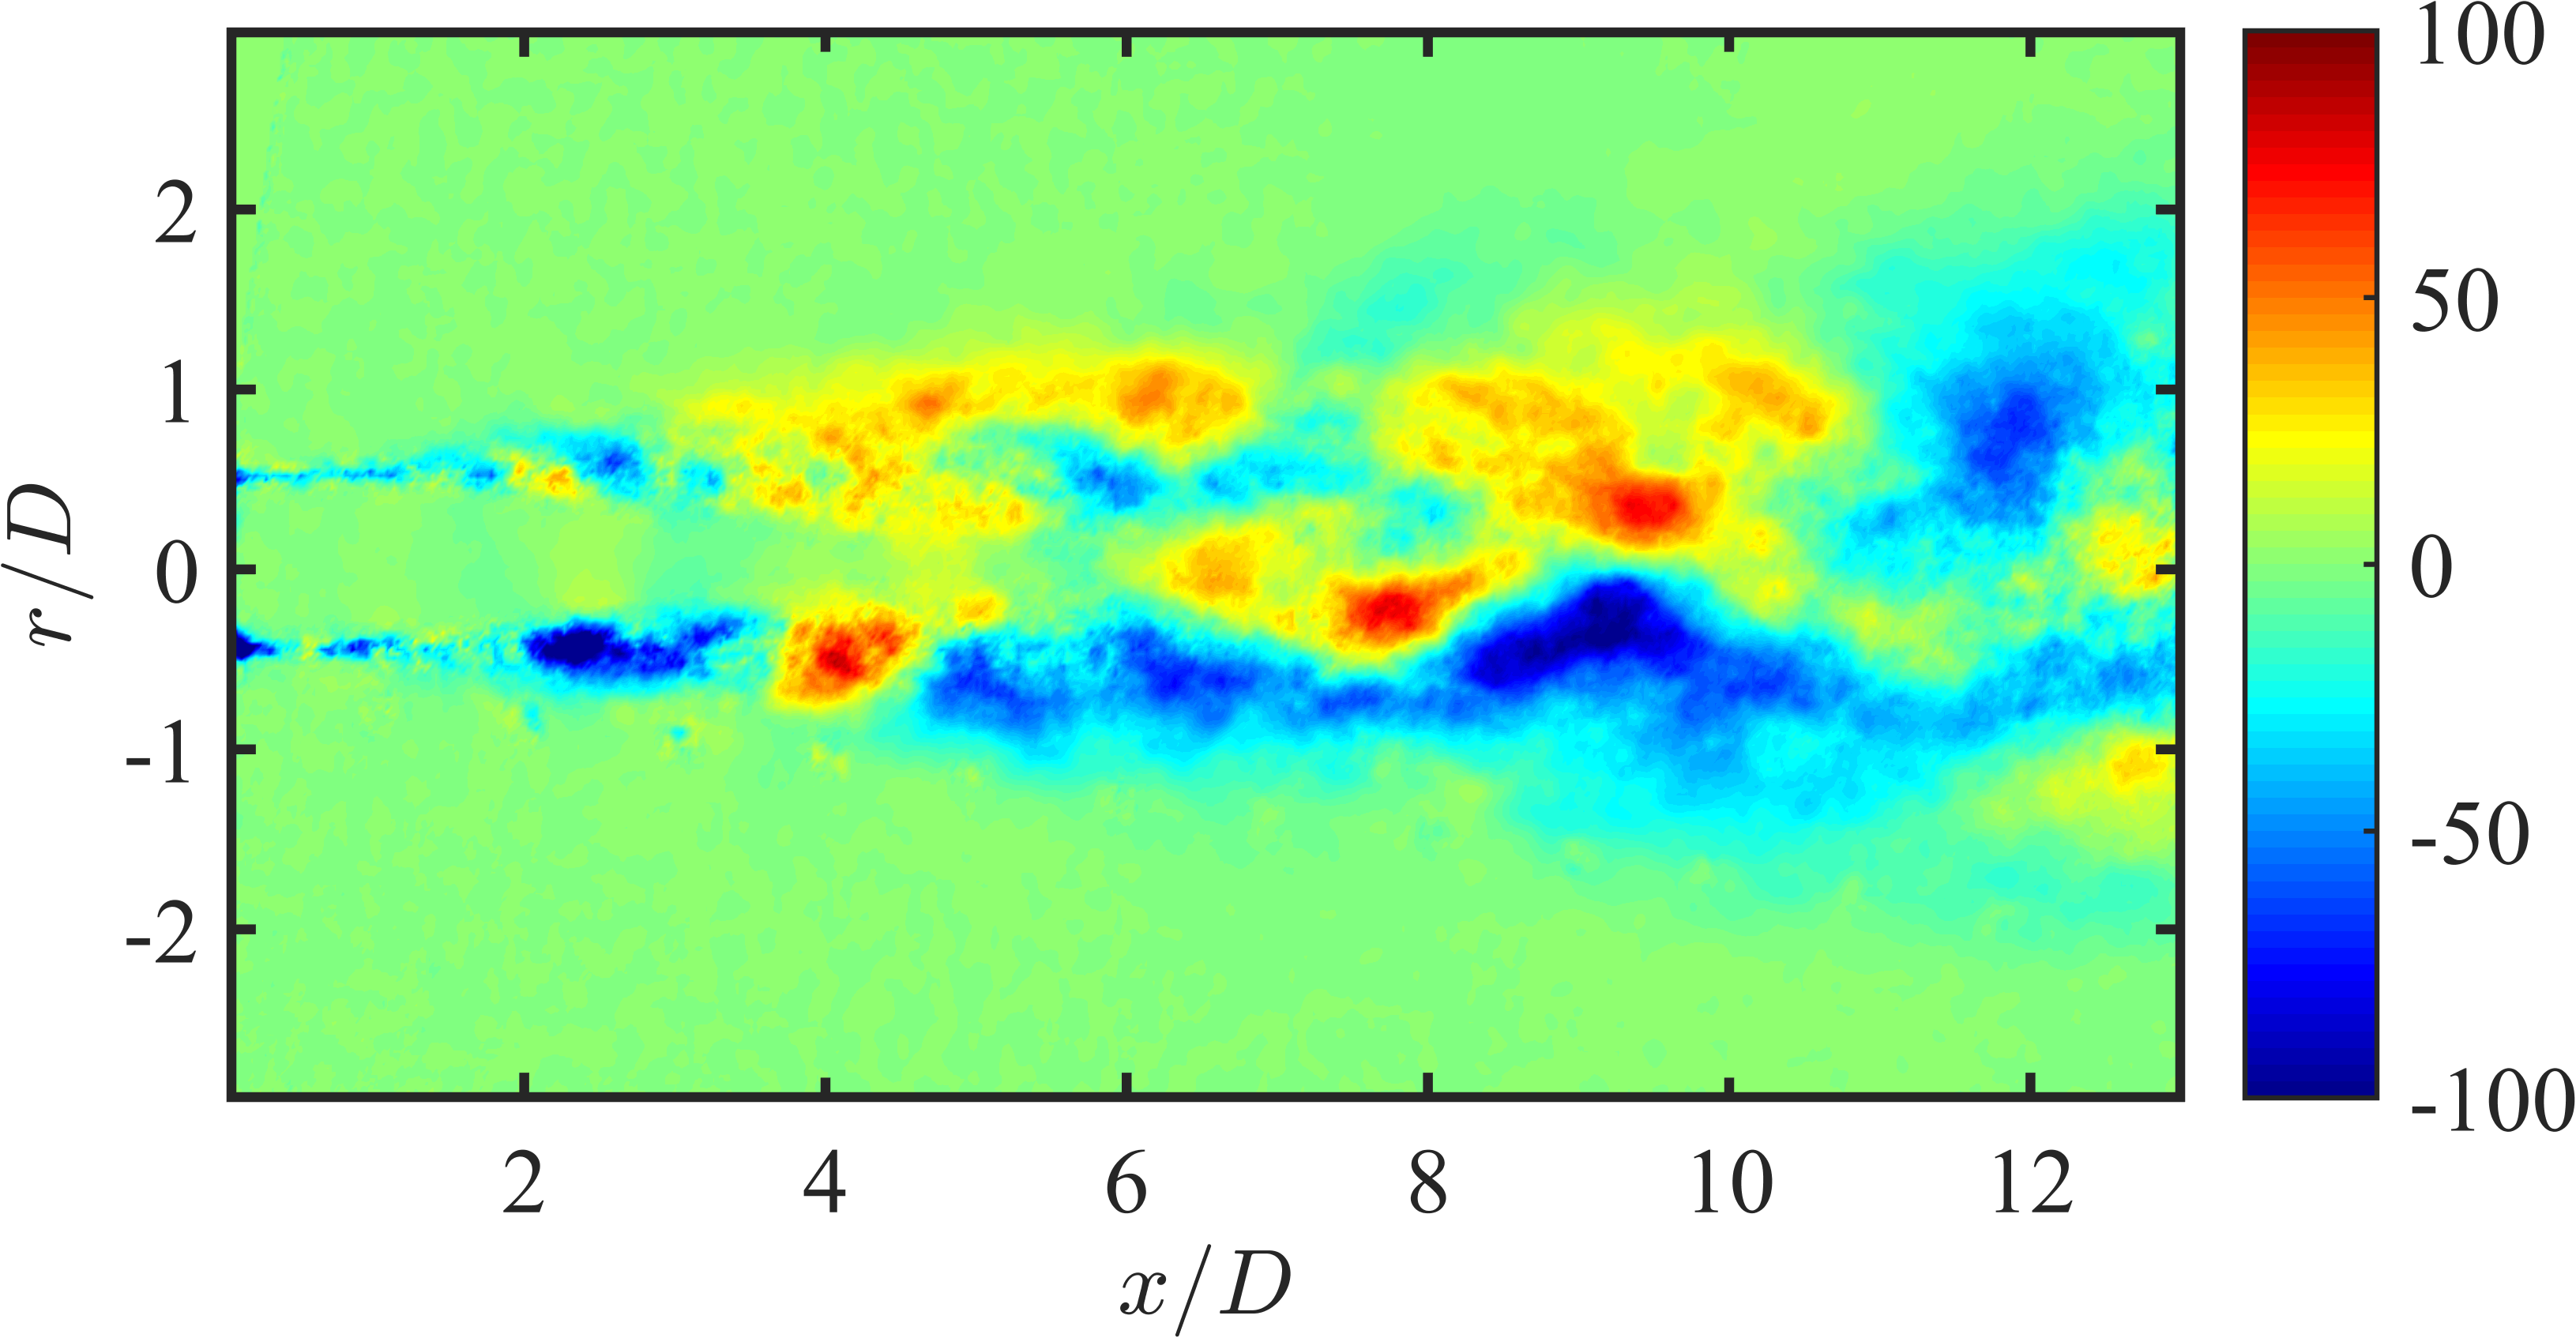
\includegraphics[width=0.95\linewidth]{Figures/ch4_Ux_POD100_v2.png}
		\caption{First 100 POD modes}
	\end{subfigure}
	\caption{Comparison of a raw instantaneous axial velocity fluctuations $St_{DF} =0.05$ (a) against the same velocity fluctuations estimated from the near-field pressure (b) and finally a reduced-order reconstruction of the raw velocity using the first 100 POD modes; units are in m/s.}
	\label{fig:ch4_SEPOD_filtering}
\end{figure}

As one would hope, the large-scale turbulent fluctuations are correctly identified by the SE-POD algorithm, and a mapping from the near-field pressure to this structures is appropriately generated.
The accuracy in the feature reproduction degrades considerably however as the scale of the turbulent eddy is reduced.
Some small-scale behavior is retained though most is filtered out, particularly the downstream region.
This was entirely expected however, as the reference signal is much more strongly damped with wavenumber than the conditional field being estimated (decay rates of $-20/3$ for the pressure field versus $-5/3$ in log-space for the velocity field).
The pressure field simply does not have the resolution to approximate the velocity field, particularly further downstream where the microphones are further from the jet centerline due to the spreading of the shear layer.
The estimated velocity fields are specifically referred to in the present work as \textit{reduced}-order rather than \textit{low}-order however.
Comparison of the estimated velocity against a reconstruction of the measured field using the most energetic 100 POD modes (of a total of 1500 POD modes corresponding to the 1500 uncorrelated velocity fields) indicates that the SE-POD algorithm retains similar (if not greater) energy levels.
An example of this is the small-scale structure observed at $x/D \simeq 4$, just outside the high-velocity region of the jet (orange-red in the figure).
This distinct structure is still visible (though smeared and slightly reduced in amplitude) in the estimated velocity, though it is basically nonexistent in the 100-mode reconstruction which contains $\sim 50$\% of the fluctuating energy (see \fig{fig:ch4_modal_energy}).
While it is unlikely that this particular structure is notably important to the acoustic emission of the jet, low modal energy modulations of the large-scale structures may be.
Hence, it is desirable to retain as much of the information as possible when estimating the flow.

As a side note, the measured velocity fields retain some experimental errors from the PIV data processing; for instance, the small pockets of zero axial velocity observed on lower shear layer (particularly for $2 < x/D < 4$) in \fig{fig:ch4_SEPOD_filtering} are non-physical and correspond to missing vectors. 
As these experimental errors will be completely uncorrelated from the pressure signals, a conditional reconstruction will have great difficulty in reproducing them; in fact they \textit{should not} map from the pressure to the velocity at all.

It is also important to be mindful that an individual POD mode may not in fact correspond to anything physically distinct in the turbulent flow - it is after all, merely a mathematical construct which is based on no \textit{a priori} information of the system under investigation.
Tinney \etal \citep{Tinney2008b} found that the modes produced by (spectral) POD had a tendency to appear in coupled pairs, and similar behavior is observed herein. 
For reference, the ten most energetic POD modes are shown in \fig{fig:ch4_St005_PODmodes} for $St_{DF} = 0.05$ and \fig{fig:ch4_St025_PODmodes} for $St_{DF} = 0.25$.
A similar behavior of the POD modes was observed between the $St_{DF} = 0.25$ and $0.35$ excitation cases; for brevity only the $St_{DF} = 0.25$ will be discussed here.
The characteristic scales of the excitation induced structures are smaller than the actual excitation period, as a result a significant amount of dead time occurs between LAFPA pulses during which the flow returns to its unperturbed state.
Because of this, analysis methods based on ensemble-averages of the velocity field show little difference between the baseline and $St_{DF} = 0.05$ excited jets (for this reason, the POD modes for the baseline jet are not shown).

For the impulsively-excited ($St_{DF} = 0.05$) jet, the dominant orthogonal modes are concentrated downstream of the end of the potential core, and it is not until mode 8 that a clear symmetric pattern about the jet centerline emerges. 
(However, it should be noted that modes 4 and 5 are very nearly mirrors of each other, and as such could produce symmetric features if coupled.)
Clearly, the excited axisymmetric structures represent only a small portion of the turbulent kinetic energy of the jet, and as such low-order representations of the flow will fail to accurately capture their dynamics.
As the excitation frequency is increased, the LAFPA-induced structures become high-energy periodic oscillations in the jet shear layer and core, and the POD modes are modified accordingly (\fig{fig:ch4_St025_PODmodes}).
Similar behaviors were found for the other periodic excitation frequencies explored in this work ($St_{DF} = 0.15, 0.35$), so for brevity only the $St_{DF} = 0.25$ will be explicitly analyzed in this section.

Strong, axisymmetric fluctuations are now observed in the jet core for the first two POD modes, which match the wavelength of the excited structures (assuming $U_c \simeq 0.7 U_j$, per the two-point near-field correlations of Crawley \etal \citep{Crawley2015}) and which peak in amplitude near the end of the potential core.
The structure of mode 2 is quite similar to that of mode 1, differing only by a phase shift of $\pi/2$. 
This is a numerical artifact produced by the downstream convection of the large-scale structures (remember that while multiple time-delays have been incorporated into the stochastic estimation algorithm, the POD was computed using a single time-delay out of necessity).
Interestingly, some of the higher modes, particularly mode 10, exhibit core fluctuations at a harmonic of the excitation wavelength.
As will be seen shortly, LAFPA excitation at this frequency yields higher-frequency structures which undergo a periodic merging to ultimately generate structures at the excitation frequency. 
These modes are capturing this process which might be highly relevant to the noise generation process. 
Lastly, even in the periodically-excited jet where the LAFPA-induced structures are the dominant POD modes, the modal energy convergence (\fig{fig:ch4_modal_energy}) of the POD modes is rather slow; as mentioned previously, 100 of the 1500 modes are required in order to capture 50\% of the total energy.
The relatively slow convergence of the modal energies, not only in the impulsively-excited jet but particularly in the periodically-excited jet, was something of a surprise for the researcher.
The convergence rate is of course a function of the number of snapshots used in the decomposition, however these results indicate that even in the excited jet, the highly coherent large-scale structures are a small fraction of the overall turbulent kinetic energy.
Again, this speaks to the necessity of accurately estimating not just the low-order modes, but the high-order as well.
\begin{figure}
	\centering
	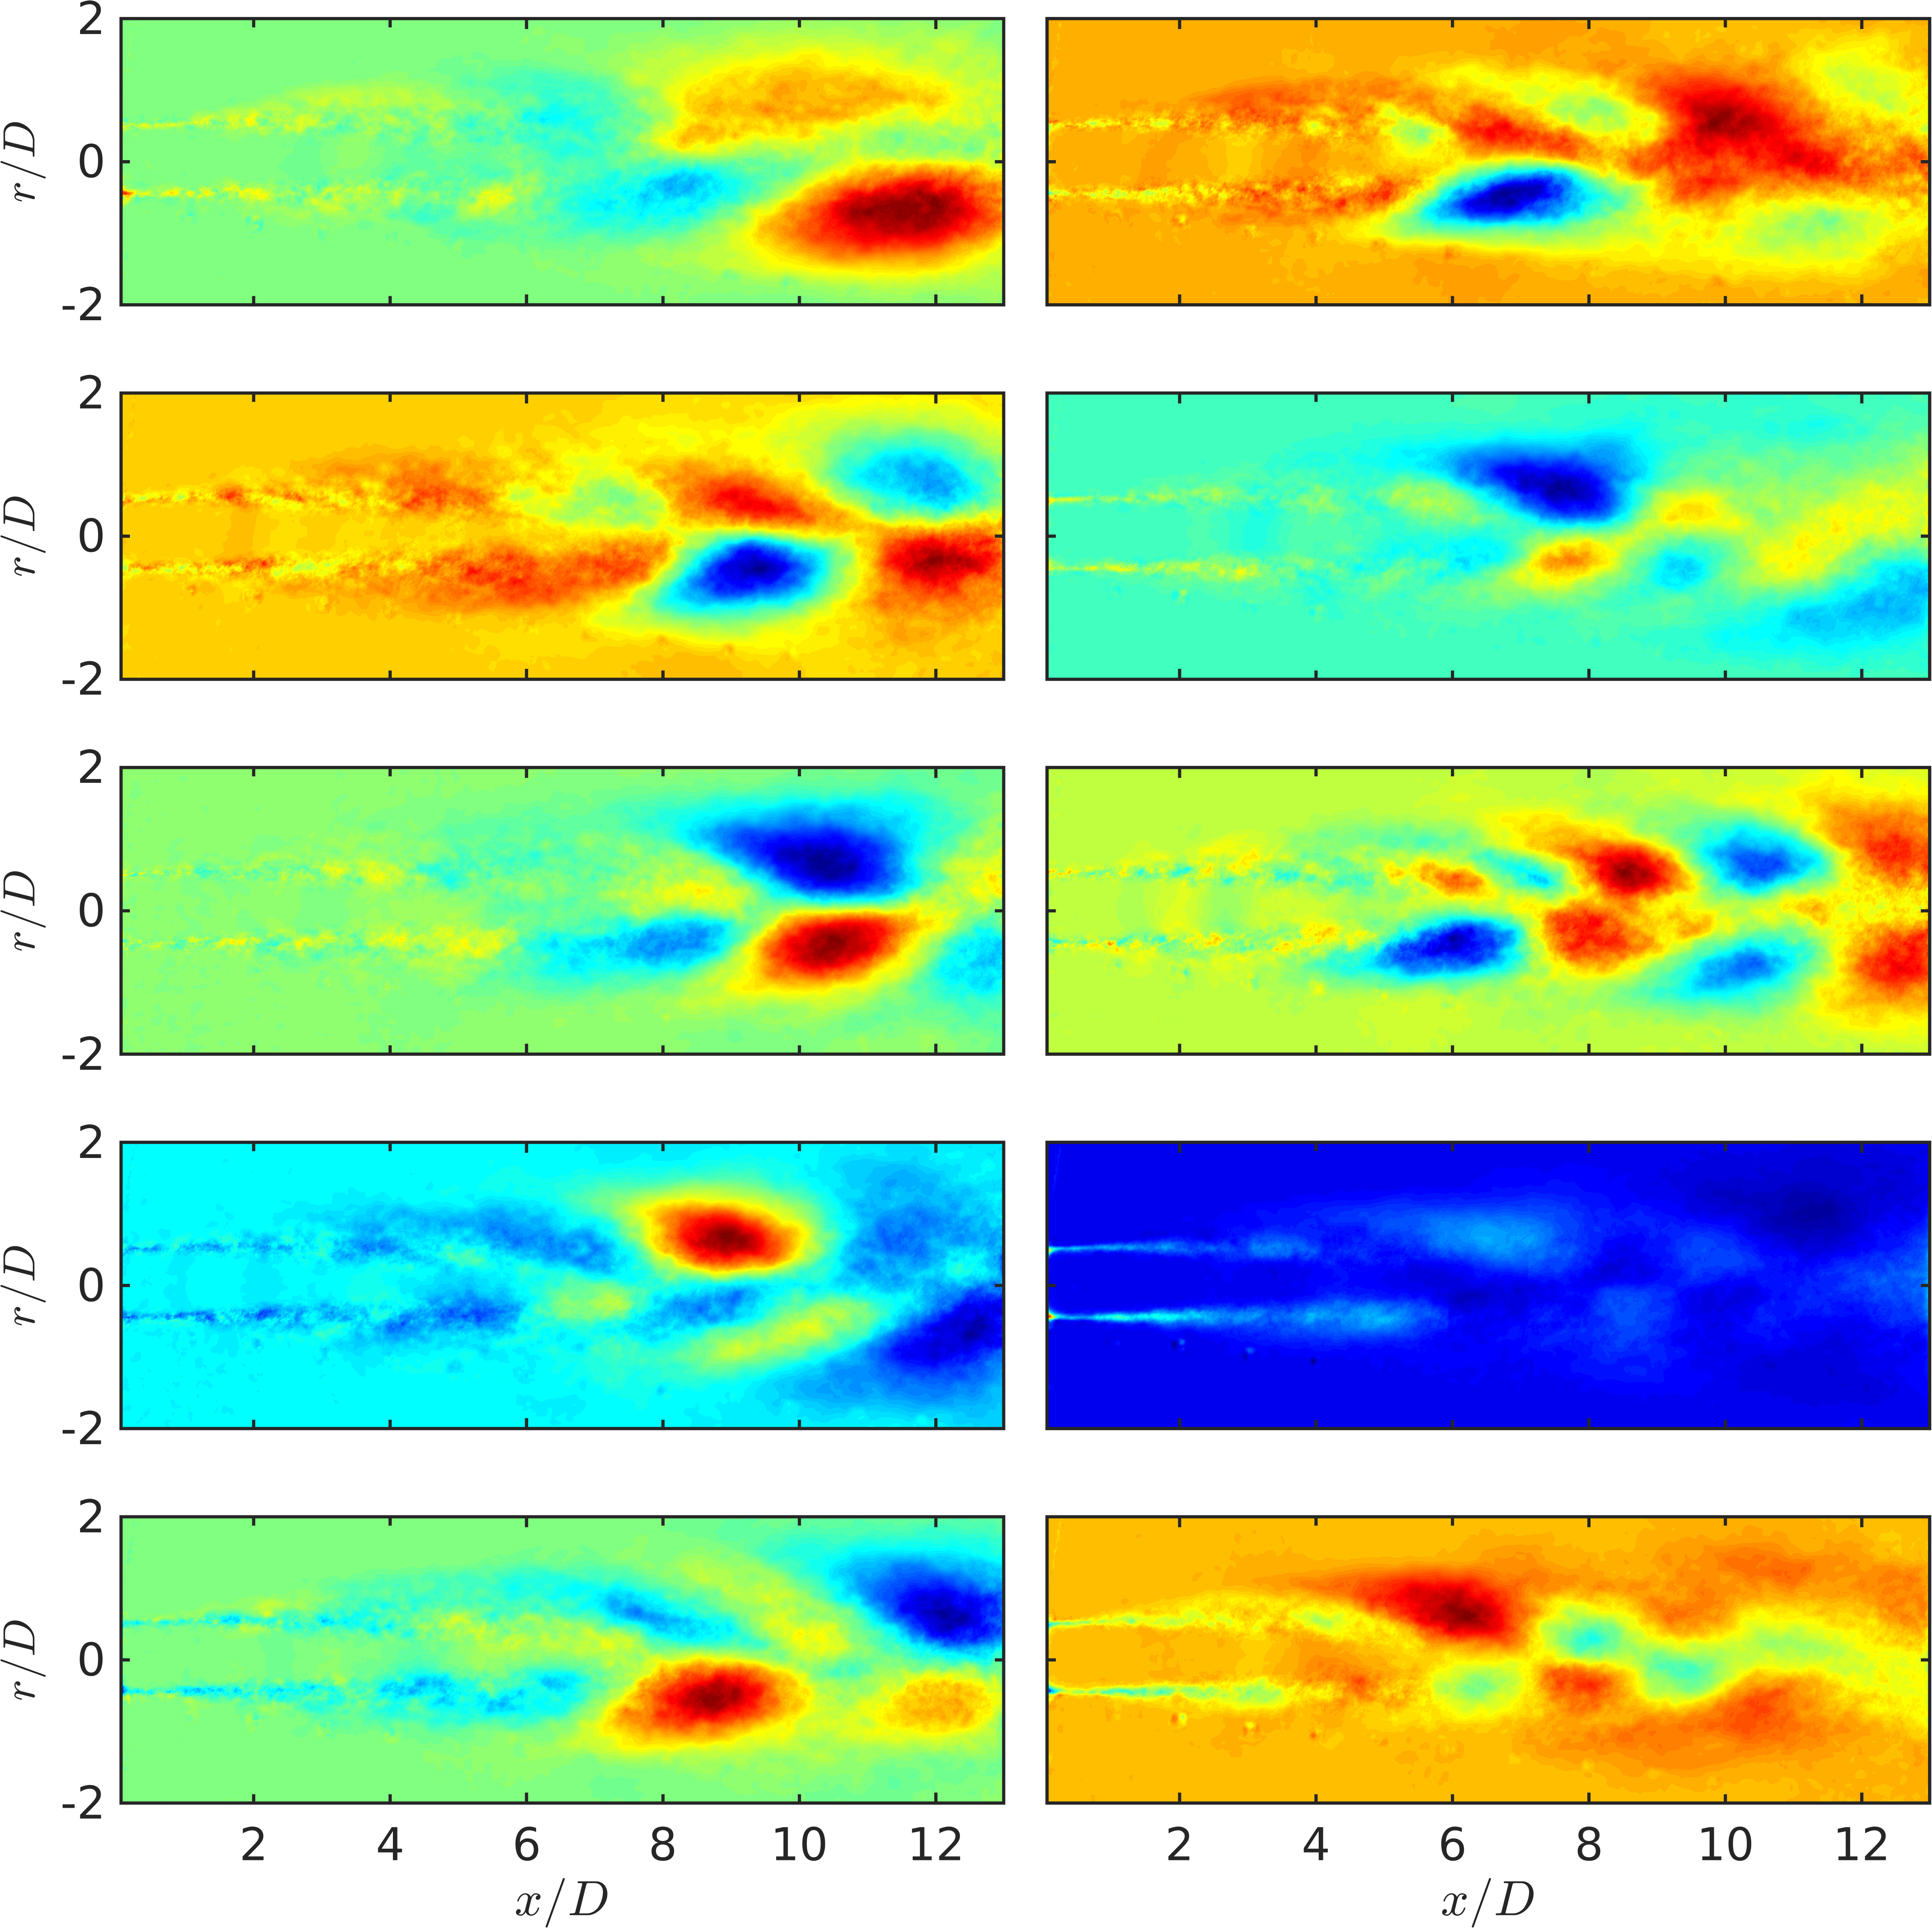
\includegraphics[width=1\linewidth]{Figures/ch4_St005_POD_Modes.png}
	\caption{First 10 POD modes (axial component only) for $St_{DF} = 0.05$, ordered top-down and then left-right.}
	\label{fig:ch4_St005_PODmodes}
\end{figure}
\begin{figure}
	\centering
	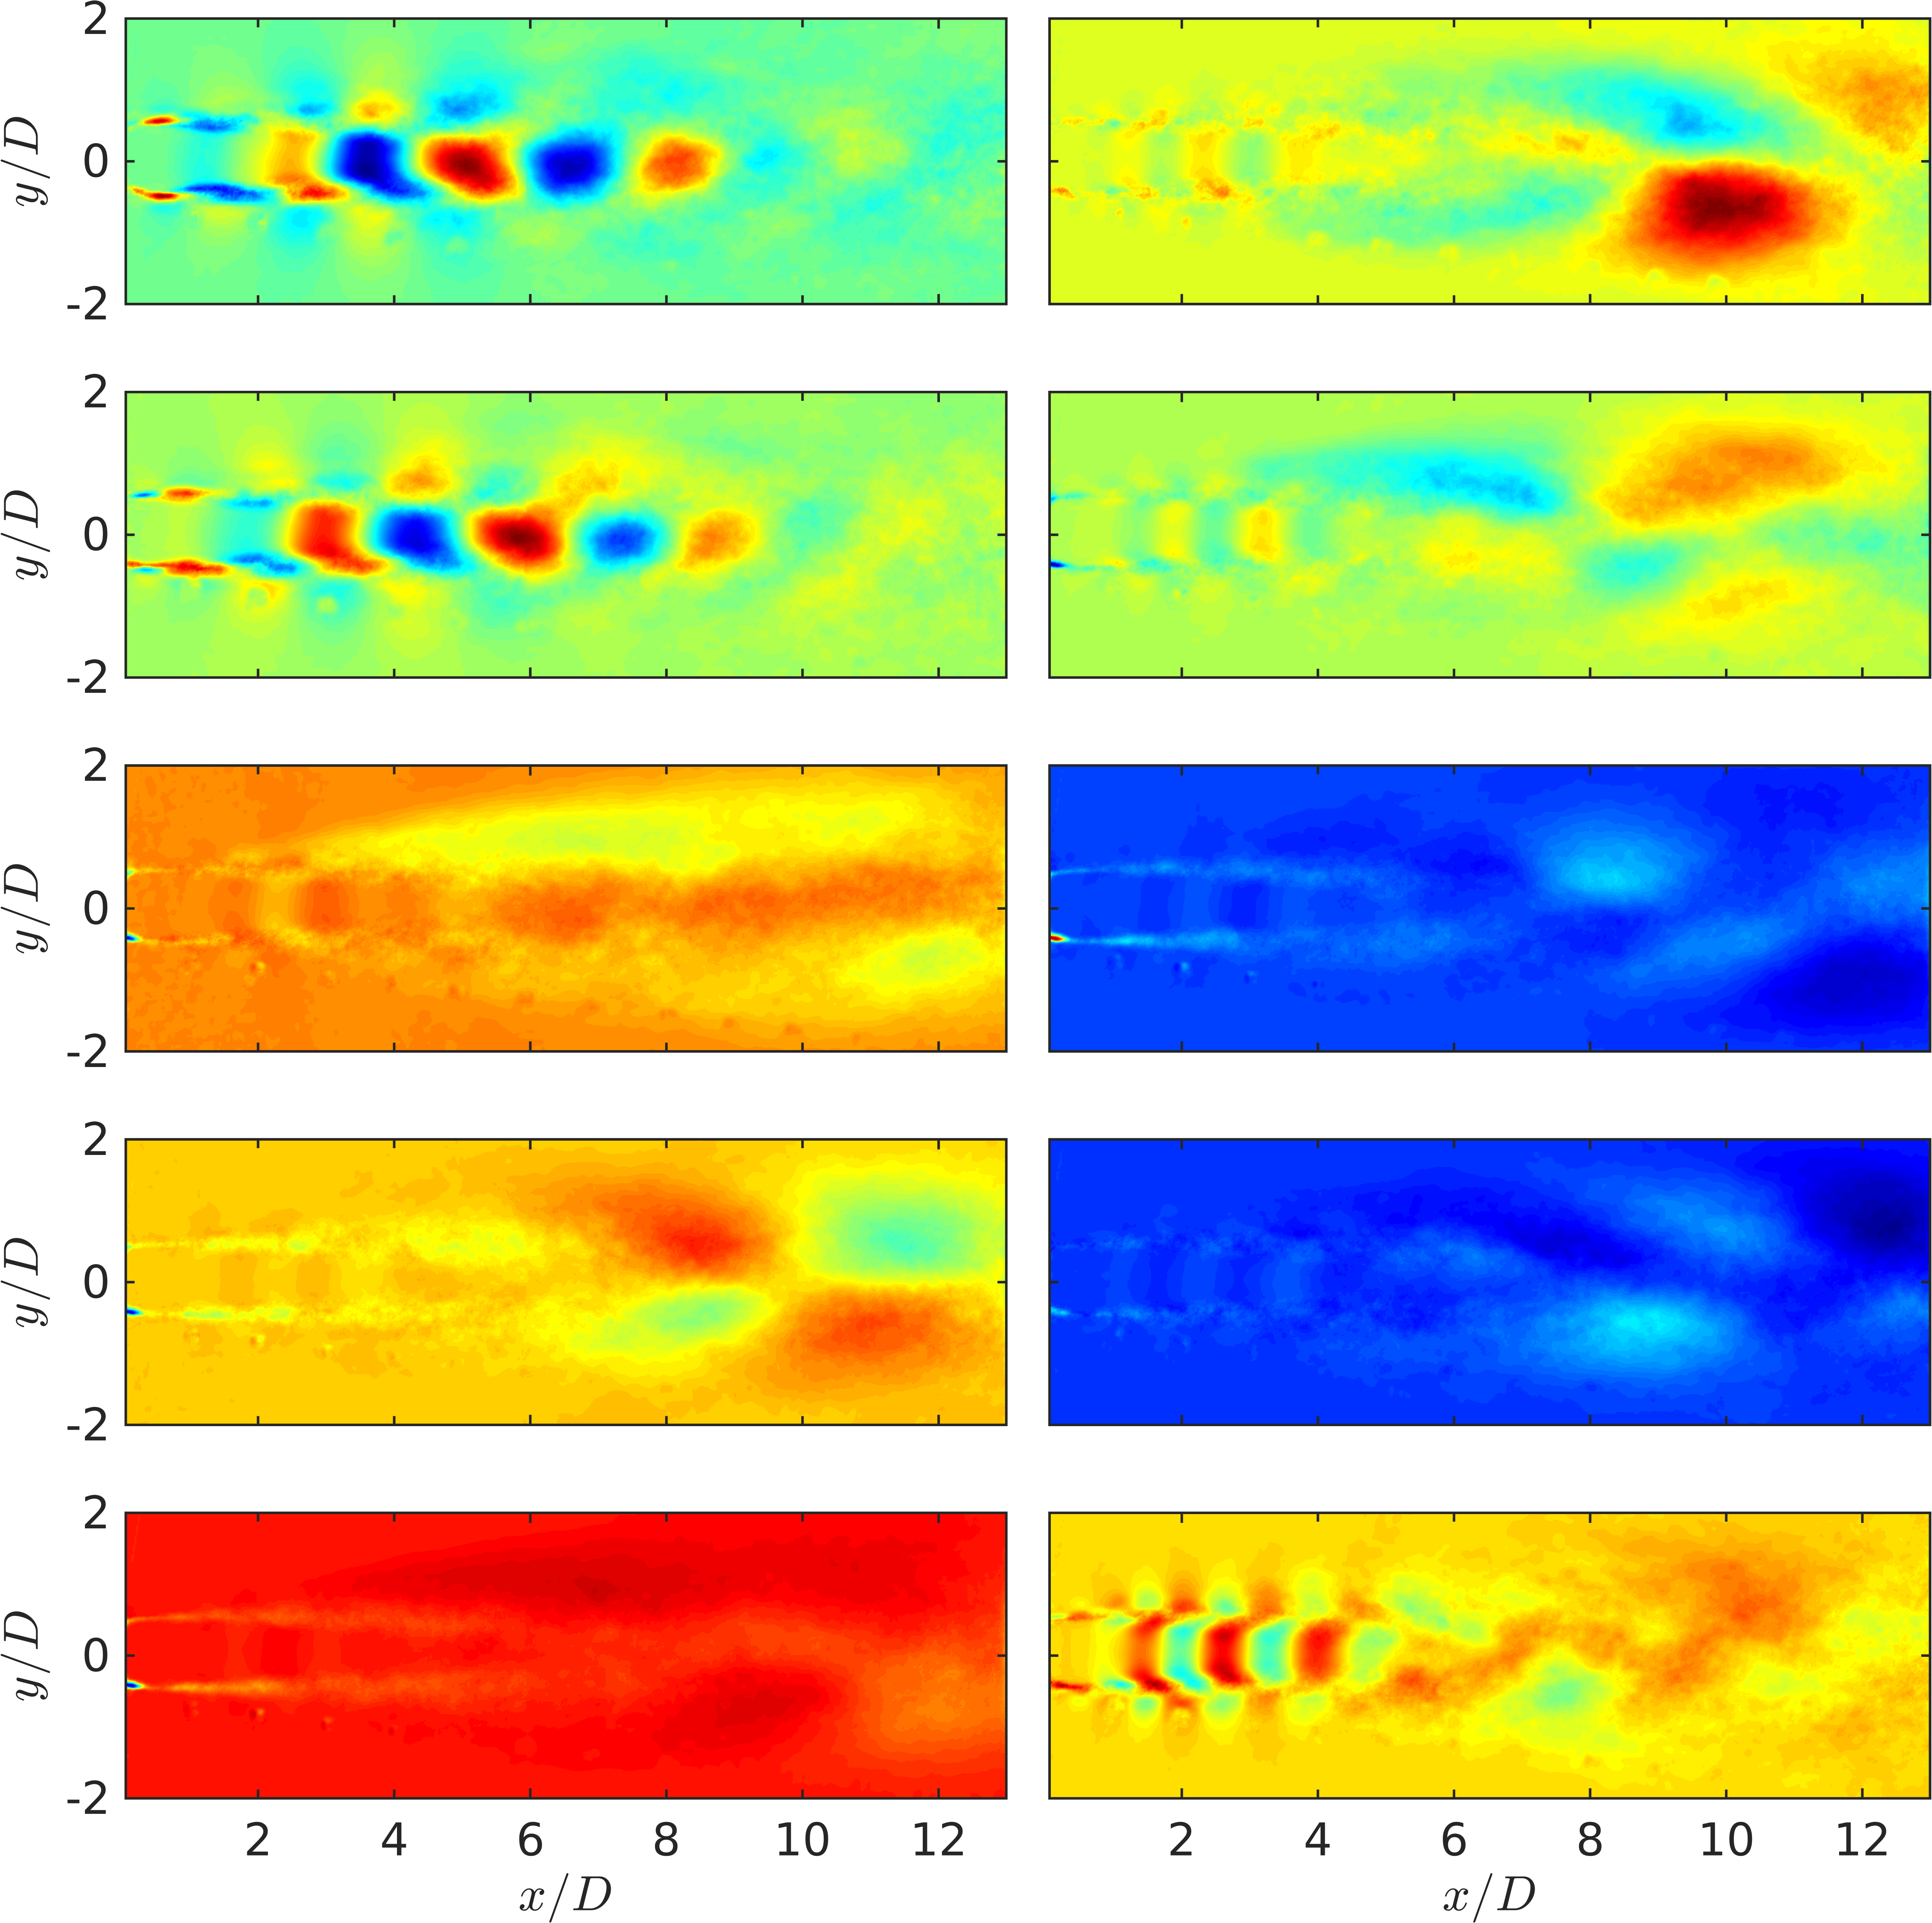
\includegraphics[width=1\linewidth]{Figures/ch4_St025_POD_Modes.png}
	\caption{First 10 POD modes (axial component only) for $St_{DF} = 0.25$, ordered top-down and then left-right.}
	\label{fig:ch4_St025_PODmodes}
\end{figure}
\begin{figure}
	\centering
	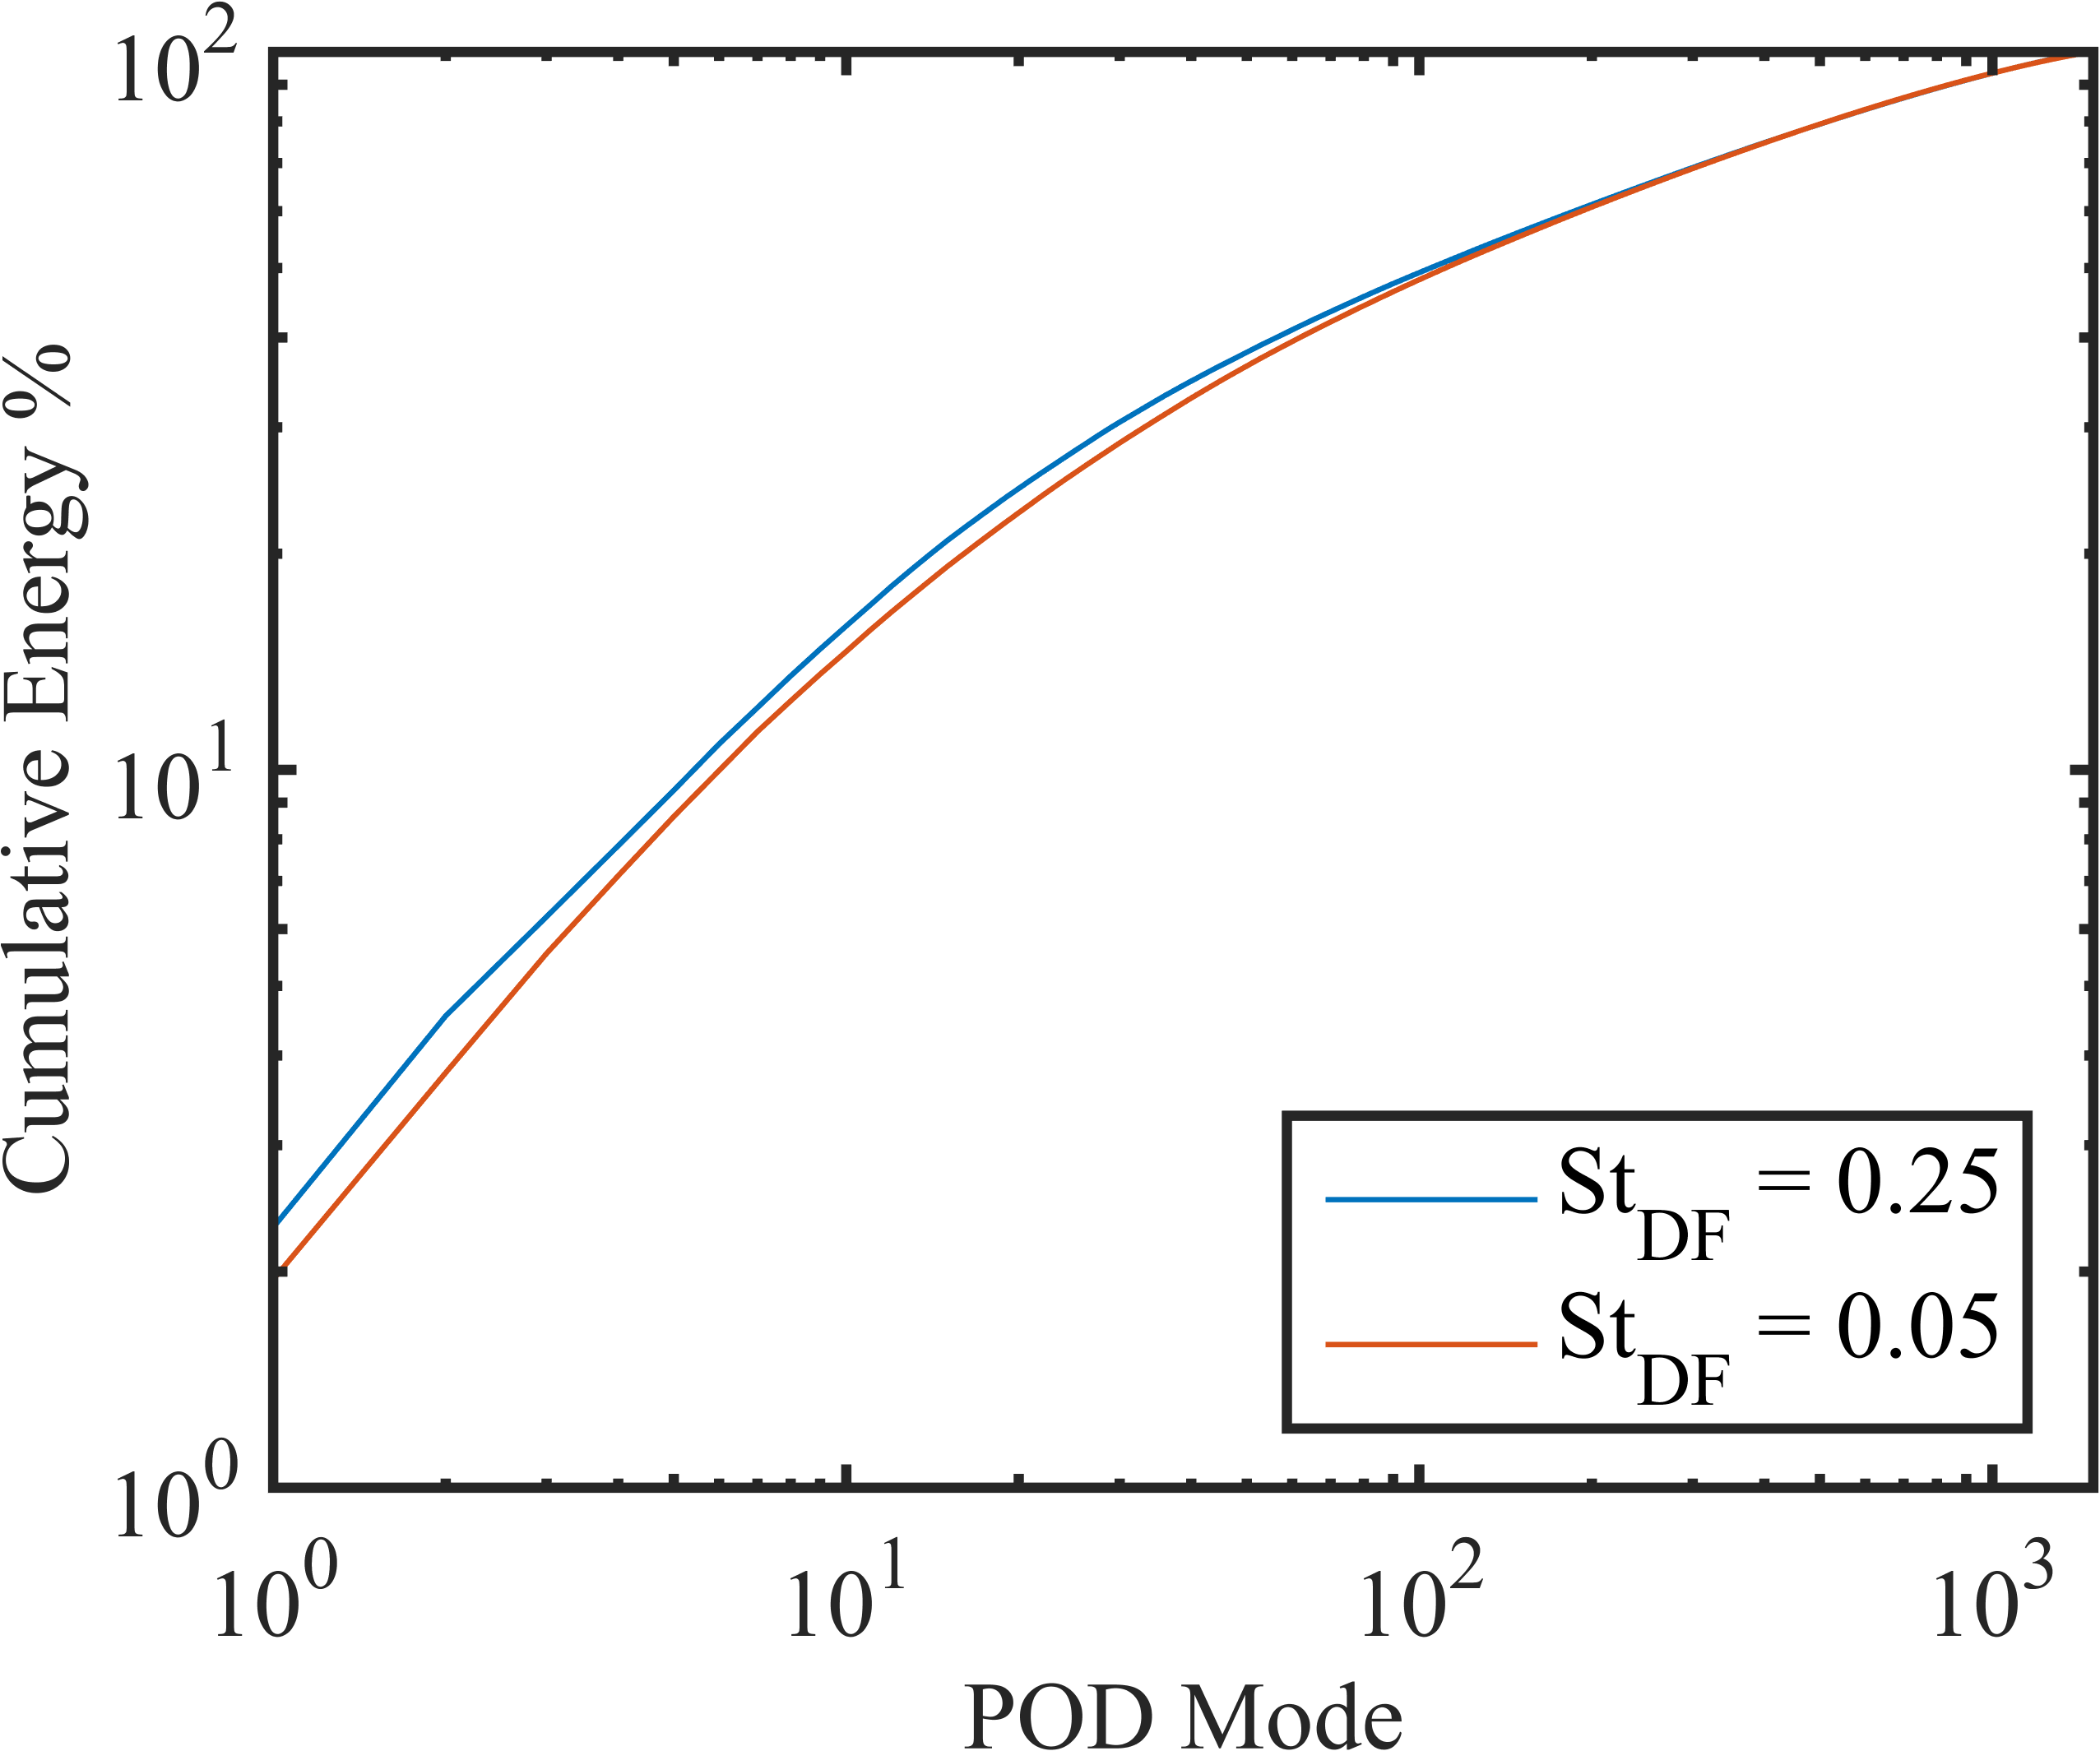
\includegraphics[width=3in]{Figures/ch4_POD_energies.png}
	\caption{POD modal energy convergence.}
	\label{fig:ch4_modal_energy}
\end{figure}


\section{Large-Scale Structure Interactions}
\subsection{Global Flow-Field Effects}
The global effects of excitation on shear layer development, both in general and in particular for LAFPAs, has been well-documented in the literature already (see Samimy \etal \citep{Samimy2012} for a review on LAFPA excitation in jets).
Therefore, only the features relevant to the current work will be briefly covered here.
Excitation produces highly-energetic structures which entrain the ambient fluid surrounding the shear layer, thus increasing mixing between the high-momentum core fluid and the ambient fluid.
As a result, the growth rate of the shear layer can be amplified significantly; this is illustrated in \fig{fig:ch4_shearlayerspreading}.
Excitation near the jet column mode ($St \simeq 0.35$) produces a rapid spreading of the initial shear layer until $x/D \simeq 5$, after which the spreading rate returns to the natural spreading rate.
(A quick note about the axial velocity fields shown in \fig{fig:ch4_shearlayerspreading}: the twelve circular regions of low velocity aligned on the outer edge of the lower shear layer are experimental artifacts. Laser reflections off of the microphones saturated the cameras, thus precluding the possibility of computing cross-correlations for these locations. Contrary to how it might appear in this figure, the microphone array is not in the flow-field, but situated behind from the cameras' point of view.)
\begin{figure}
	\centering
	\begin{subfigure}{0.75\textwidth}
		\centering
		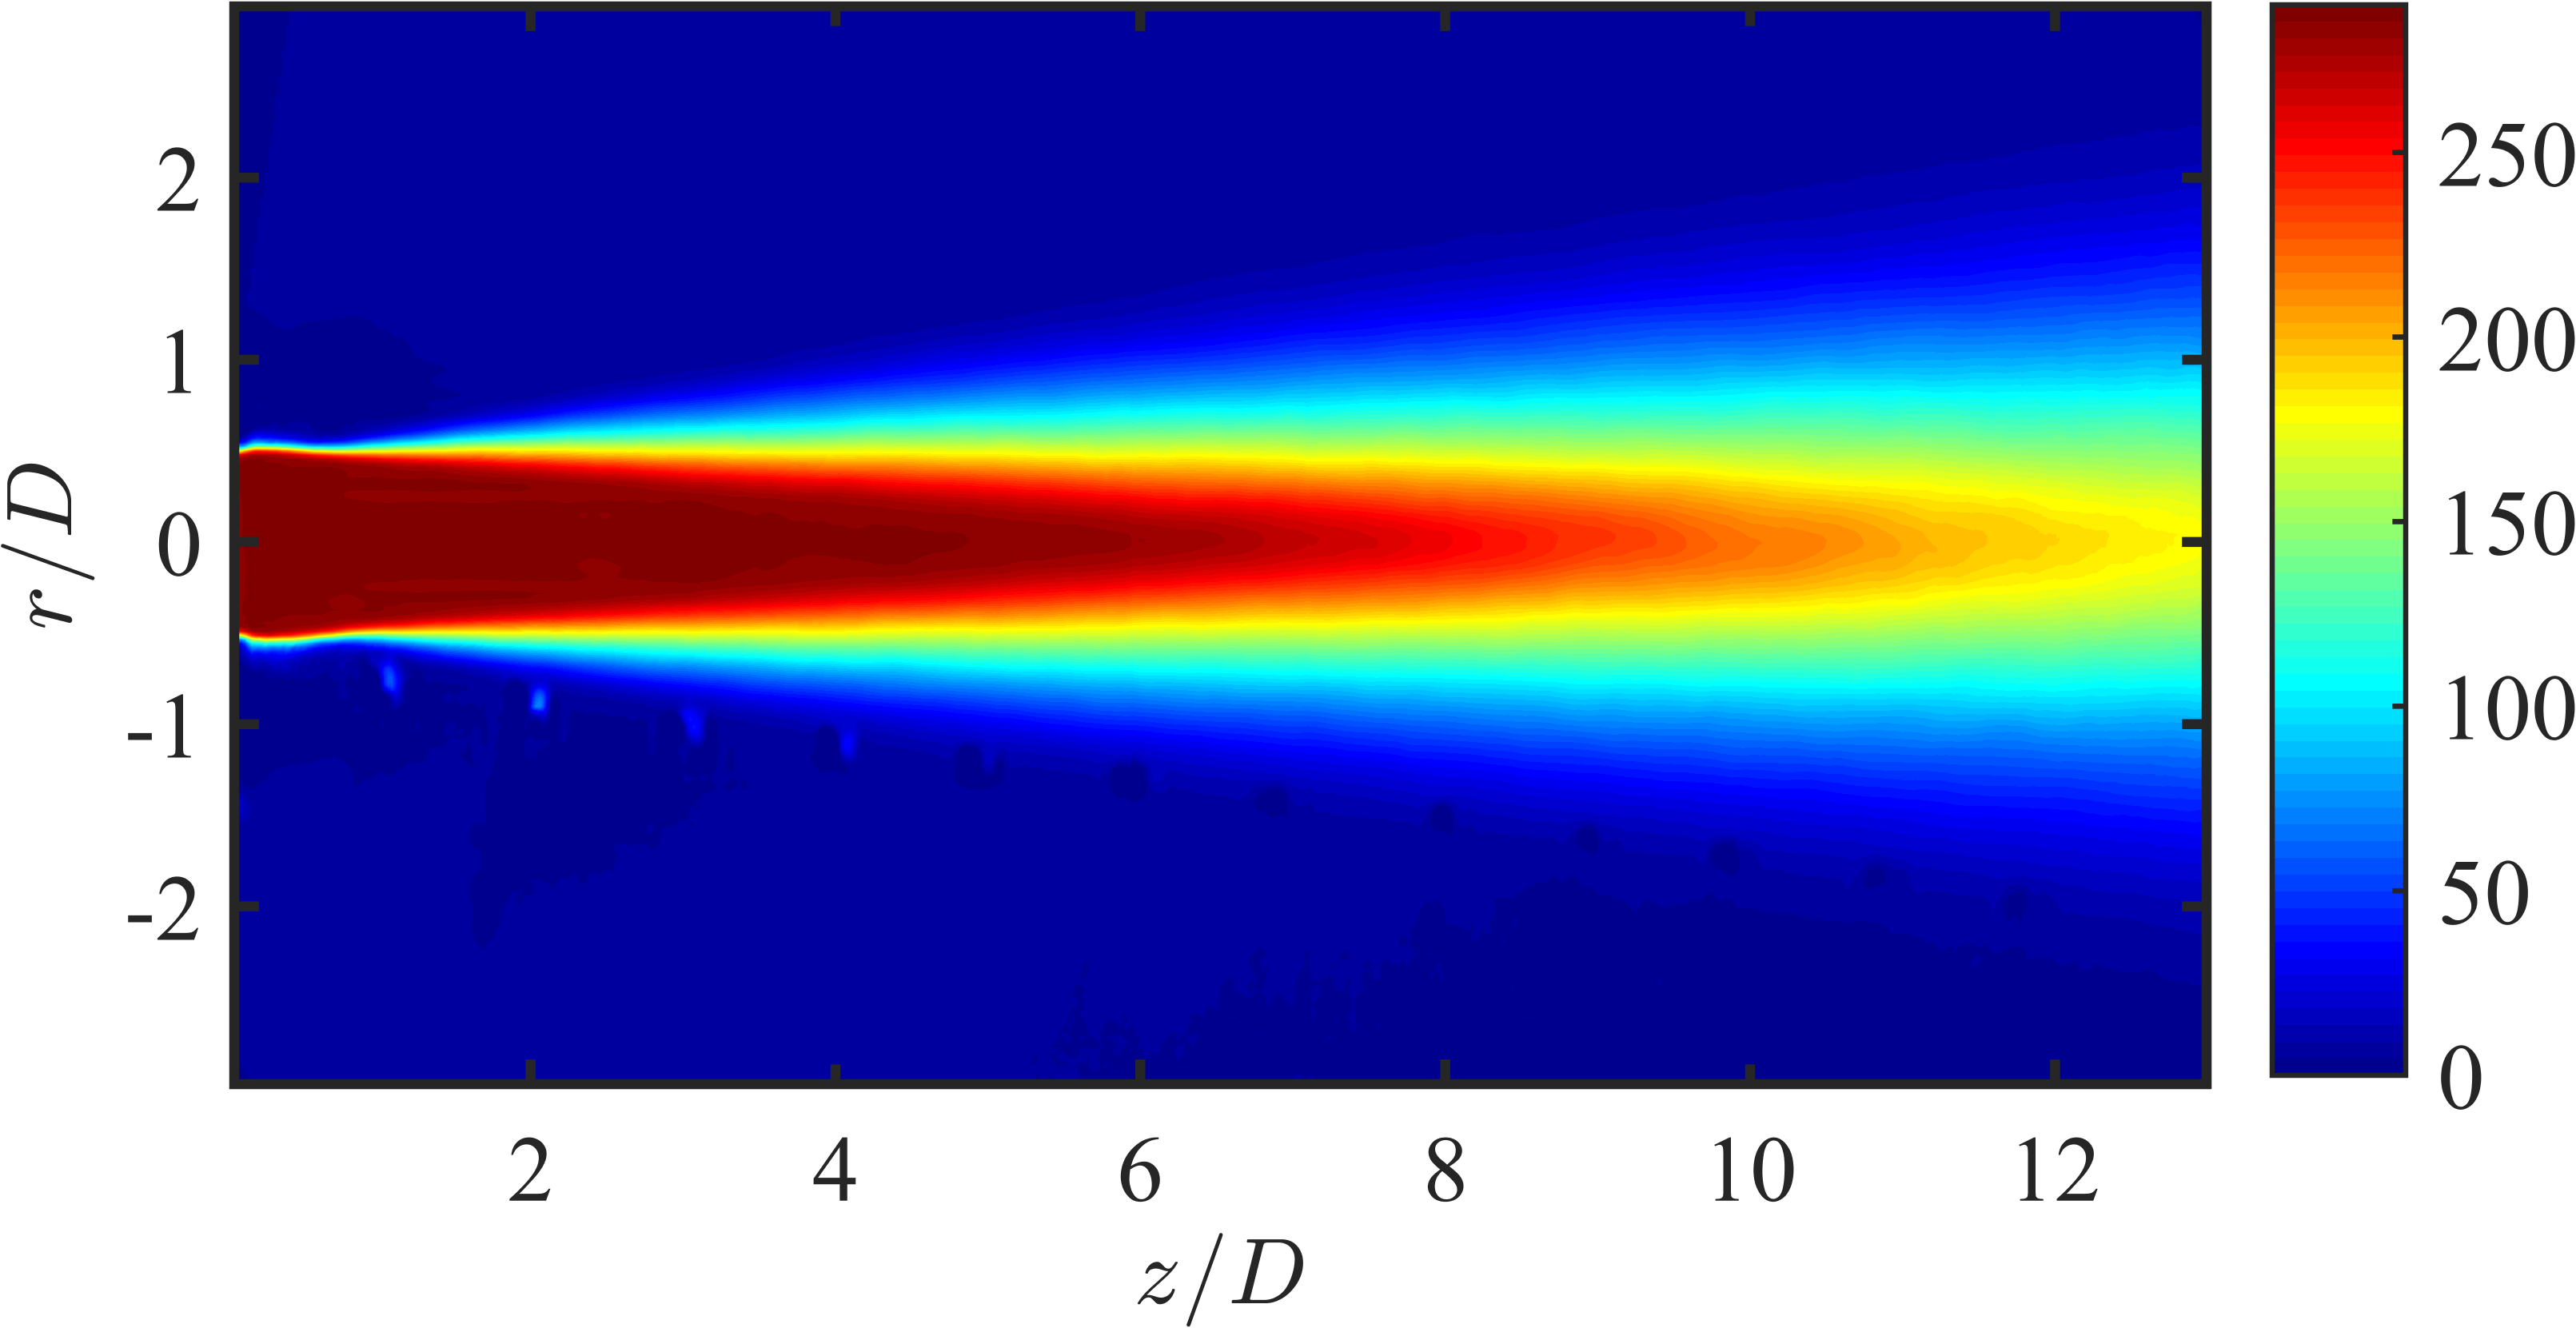
\includegraphics[width=0.95\linewidth]{Figures/ch4_St000_Um.png}
		\caption{Baseline}
	\end{subfigure}\\
	\begin{subfigure}{0.75\textwidth}
		\centering
		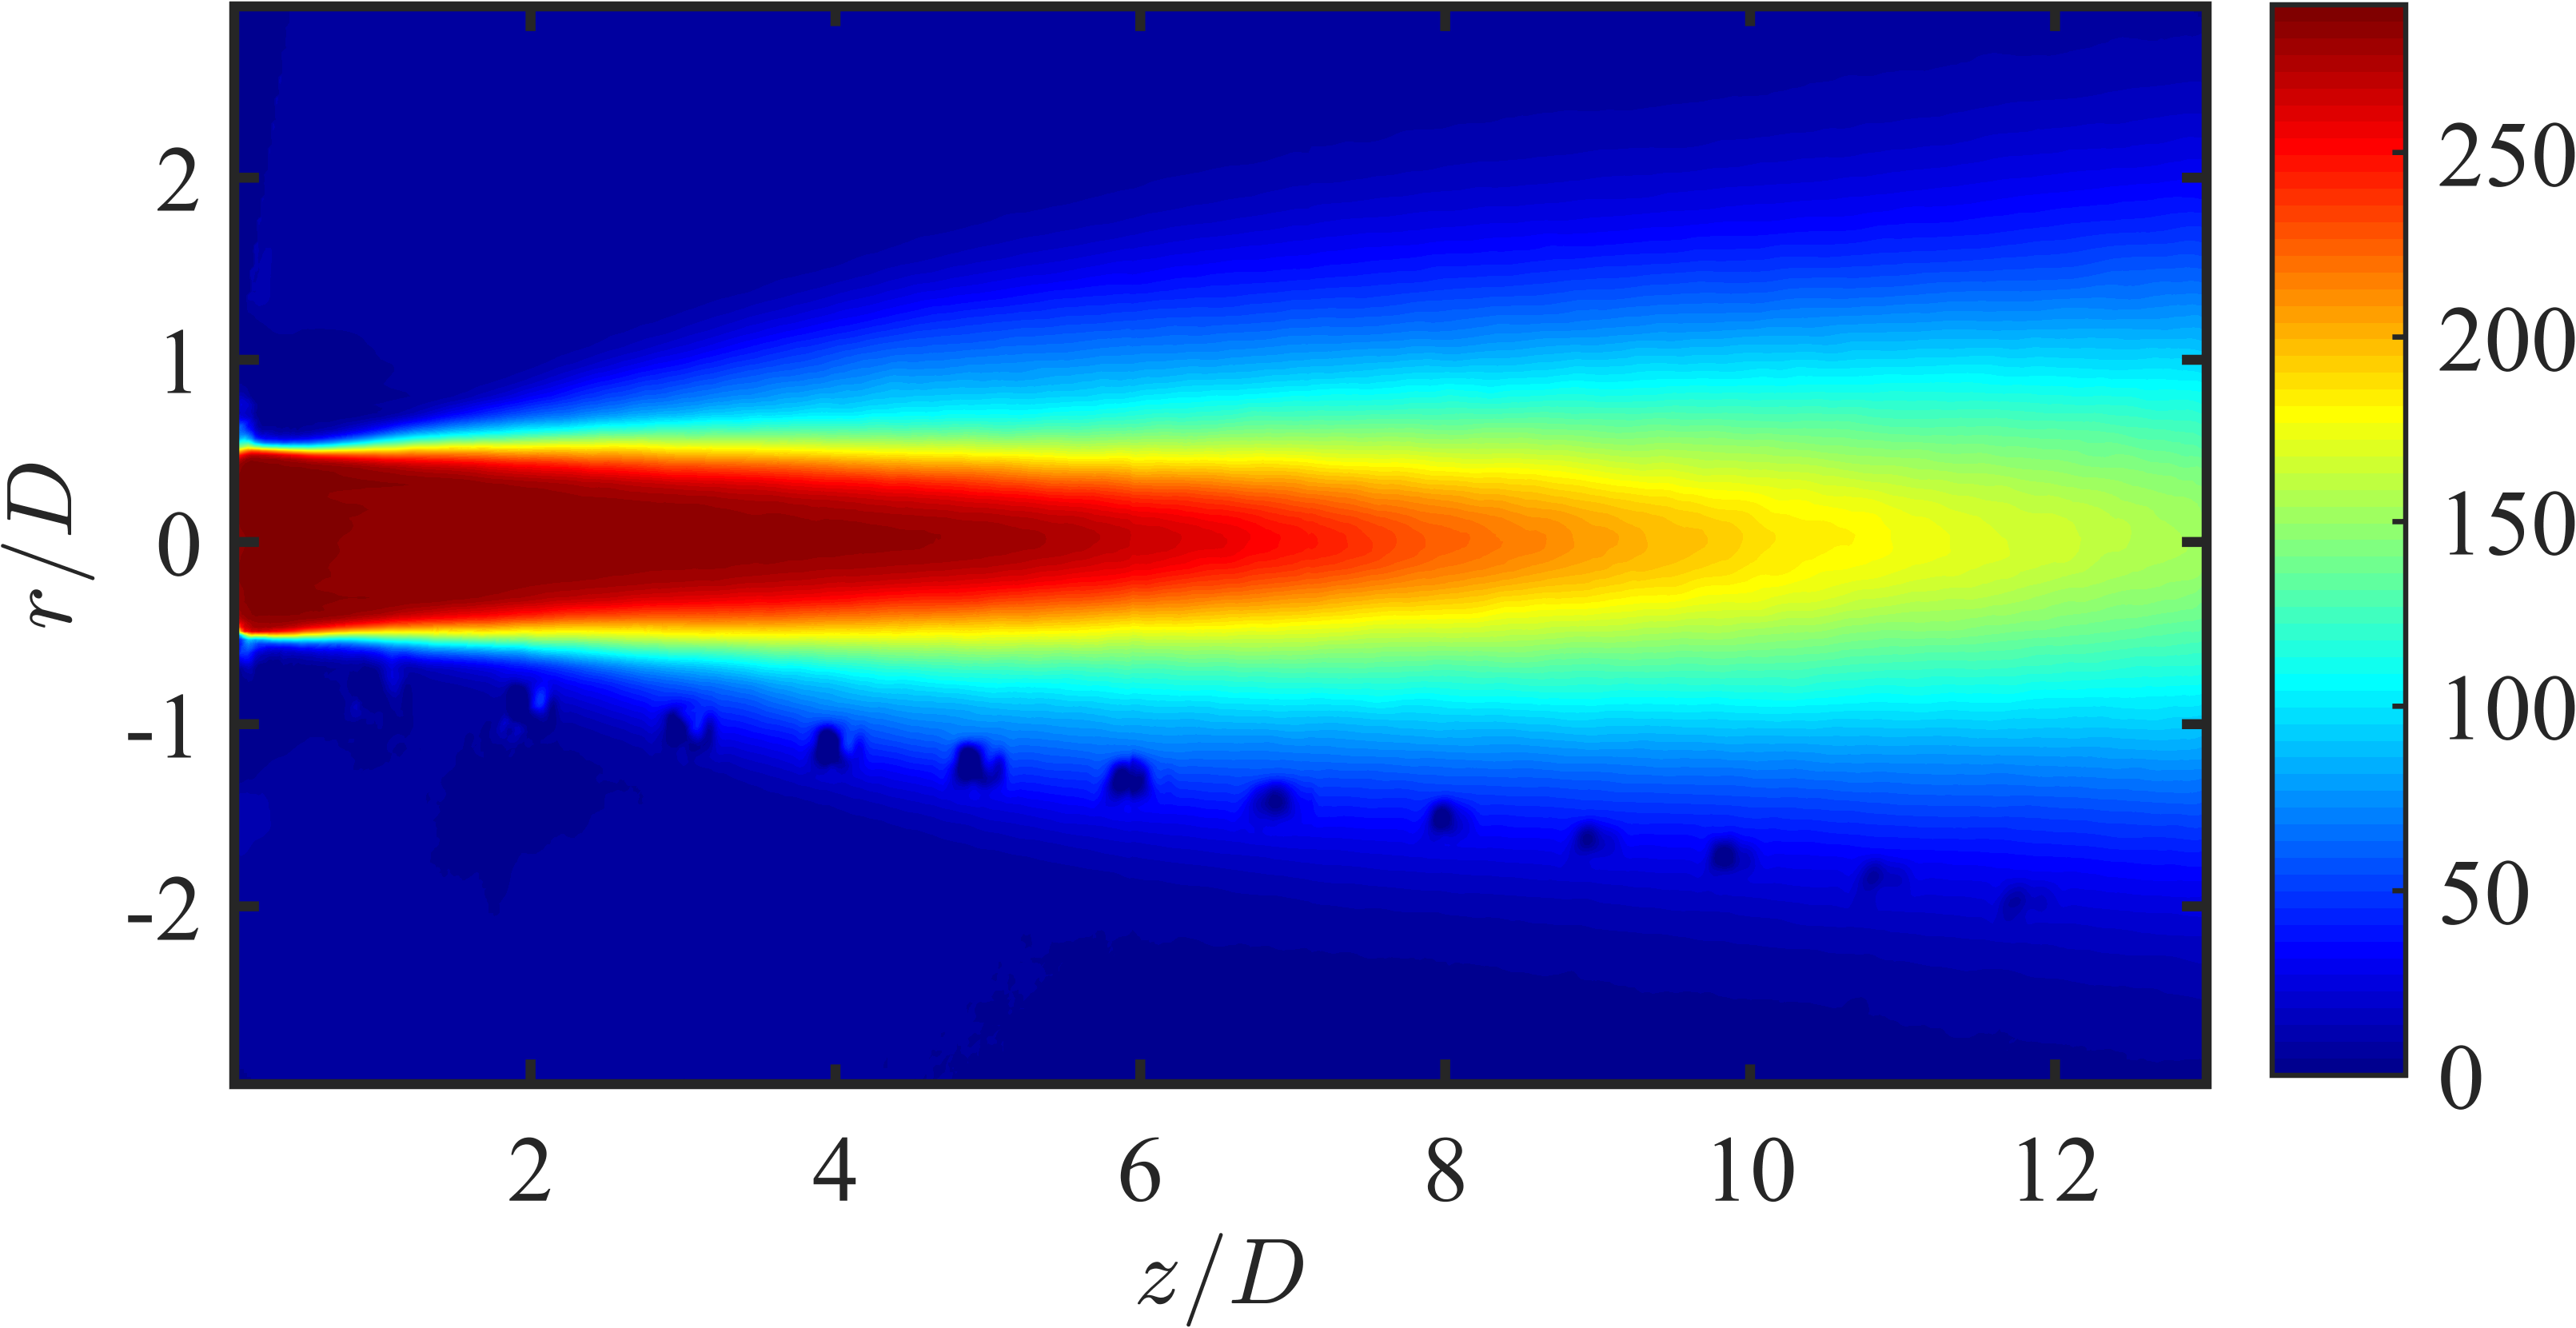
\includegraphics[width=0.95\linewidth]{Figures/ch4_St035_Um.png}
		\caption{$St_{DF} = 0.35$}
	\end{subfigure}
	\caption{Effect of excitation on the shear layer spreading rate, as visualized by the axial component of the velocity field.}
	\label{fig:ch4_shearlayerspreading}
\end{figure}

The increased mixing also affects the high-velocity side of the shear layer, resulting in a reduction in the length of the potential core.
In \fig{fig:ch4_centerlinemach}, the time-averaged centerline Mach number for each excitation case (as well as the natural jet) has been plotted as a function of axial distance.
A slow progression in the location of the end of the potential core is clearly evident, with it shifting upstream from $x/D \simeq 6$ eventually to $x/D \simeq 5$ as the excitation Strouhal number nears the jet preferred frequency of $St_{DF} \simeq 0.35$ (though not shown here, above this excitation frequency the effect is reduced).
The end of the potential core is of particular interest for the current work, as previous researchers have indicated that the dominant noise generation mechanism is associated with the violent breakdown of large-scale axisymmetric structures as they pass through this location \citep{Hileman2005}.
The two-point correlations of \sect{sect:nearfield}, which identified the dominant noise source region as occurring near the end of the potential core, hint at this as well.

The breakdown of the large-scale axisymmetric structures occurs because as the shear layers merge, the interface between the interior sides of the ring vortex becomes highly unstable, so any small perturbations quickly grow and destroy the vortex.
The exact location at which this breakdown occurs is ultimately going to be a function of structure growth rate, as larger structures will self-interact further upstream.
The location of the end of the potential core is therefore dependent on the passage of the large-scale structures, and hence is not strictly constant in time.
Therefore, an axial shift in the time-averaged acoustic source (or a source location not exactly at the time-averaged end of potential core) is not necessarily reflective of a changing source mechanism, but may instead simply indicate that the source mechanism is now occurring at a different location.
\begin{figure}
	\centering
	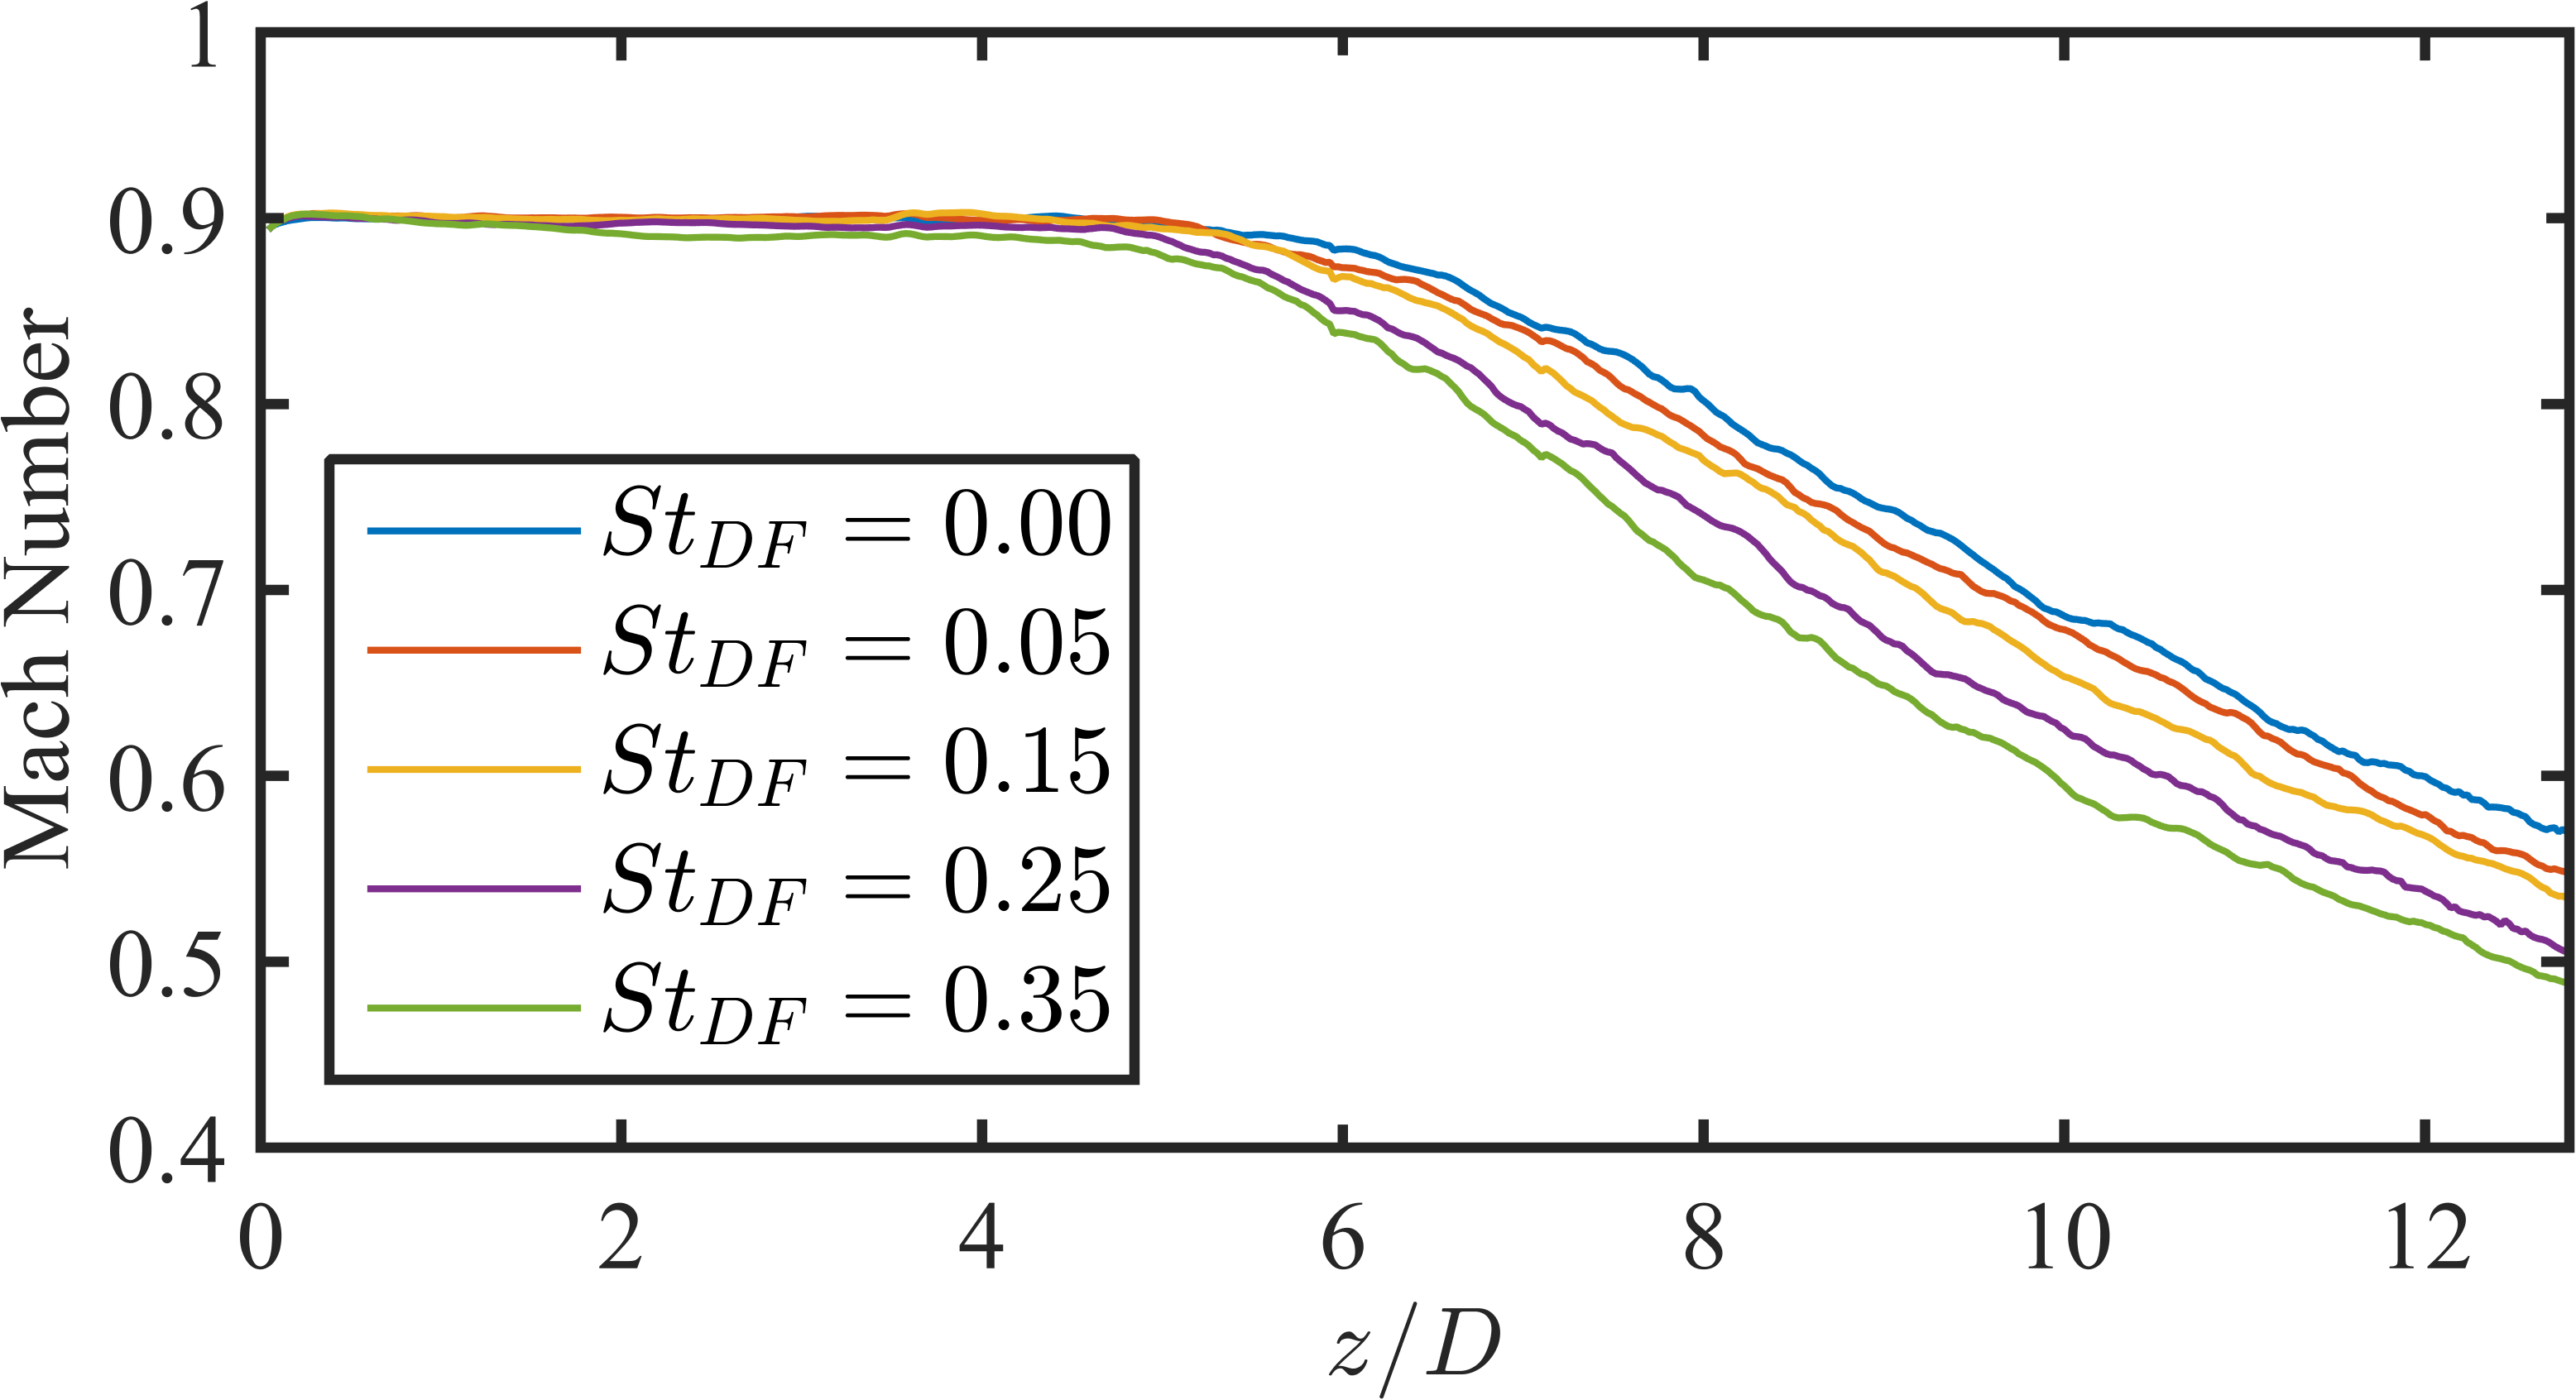
\includegraphics[width = 3.5in]{Figures/ch4_centerlineMach.png}
	\caption{Centerline Mach number for all excitation cases; baseline jet is indicated by `0.00'.}
	\label{fig:ch4_centerlinemach}
\end{figure}

\subsection{Large-Scale Structure Disintegration}
Hileman \etal \citep{Hileman2005} investigated the evolution and interactions of large-scale structures and ultimately how these relate to the noise generation process in a supersonic, ideally-expanded jet by combining time-resolved flow visualizations with a three-dimensional microphone array.
Their results showed that the dominant noise was being generated near the end of the potential core, in the region where the shear layers merged.
Large-amplitude, highly-intermittent acoustic events were found to be associated with a fluctuation in the length of the potential core, which the authors ultimately speculated was related to the passage and finally the rapid disintegration of large-scale coherent structures just downstream of the end of the potential core.
The results of \sect{sect:nearfield} also indicated that the region upstream of the end of the potential core was responsible for the dominant acoustic generation in a subsonic jet, at least to low angles with respect to the jet axis.
The dynamics of the large-scale structures in this region, namely the structure disintegration, are therefore of particular concern to the current work.

Vortex identification was performed by computing the swirling strength at each instance in the estimated velocity field; details and justification for this method can be found in Adrian \etal \citep{Adrian2000}.
The evolution of the impulsively excited ($St_{DF} = 0.05$) vortex ring has be tracked in \fig{fig:ch4_impulse_structure_disintegration}.
For ease of visualization, a two-dimensional, five-point boxcar filter was applied to the estimated velocity fields prior to computing the swirling strength, and the results have been phase-averaged based on the recorded LAFPA trigger signal over roughly 30 excitation periods.
Lastly, a solid red line has been overlain to approximately match the convective velocity of the structures.
Only a select number of phases are shown here, as a significant amount of dead time between excitations occurs due to the mismatch in the spatial and temporal characteristic frequencies of the large-scale structures.
\begin{figure}
	\centering
	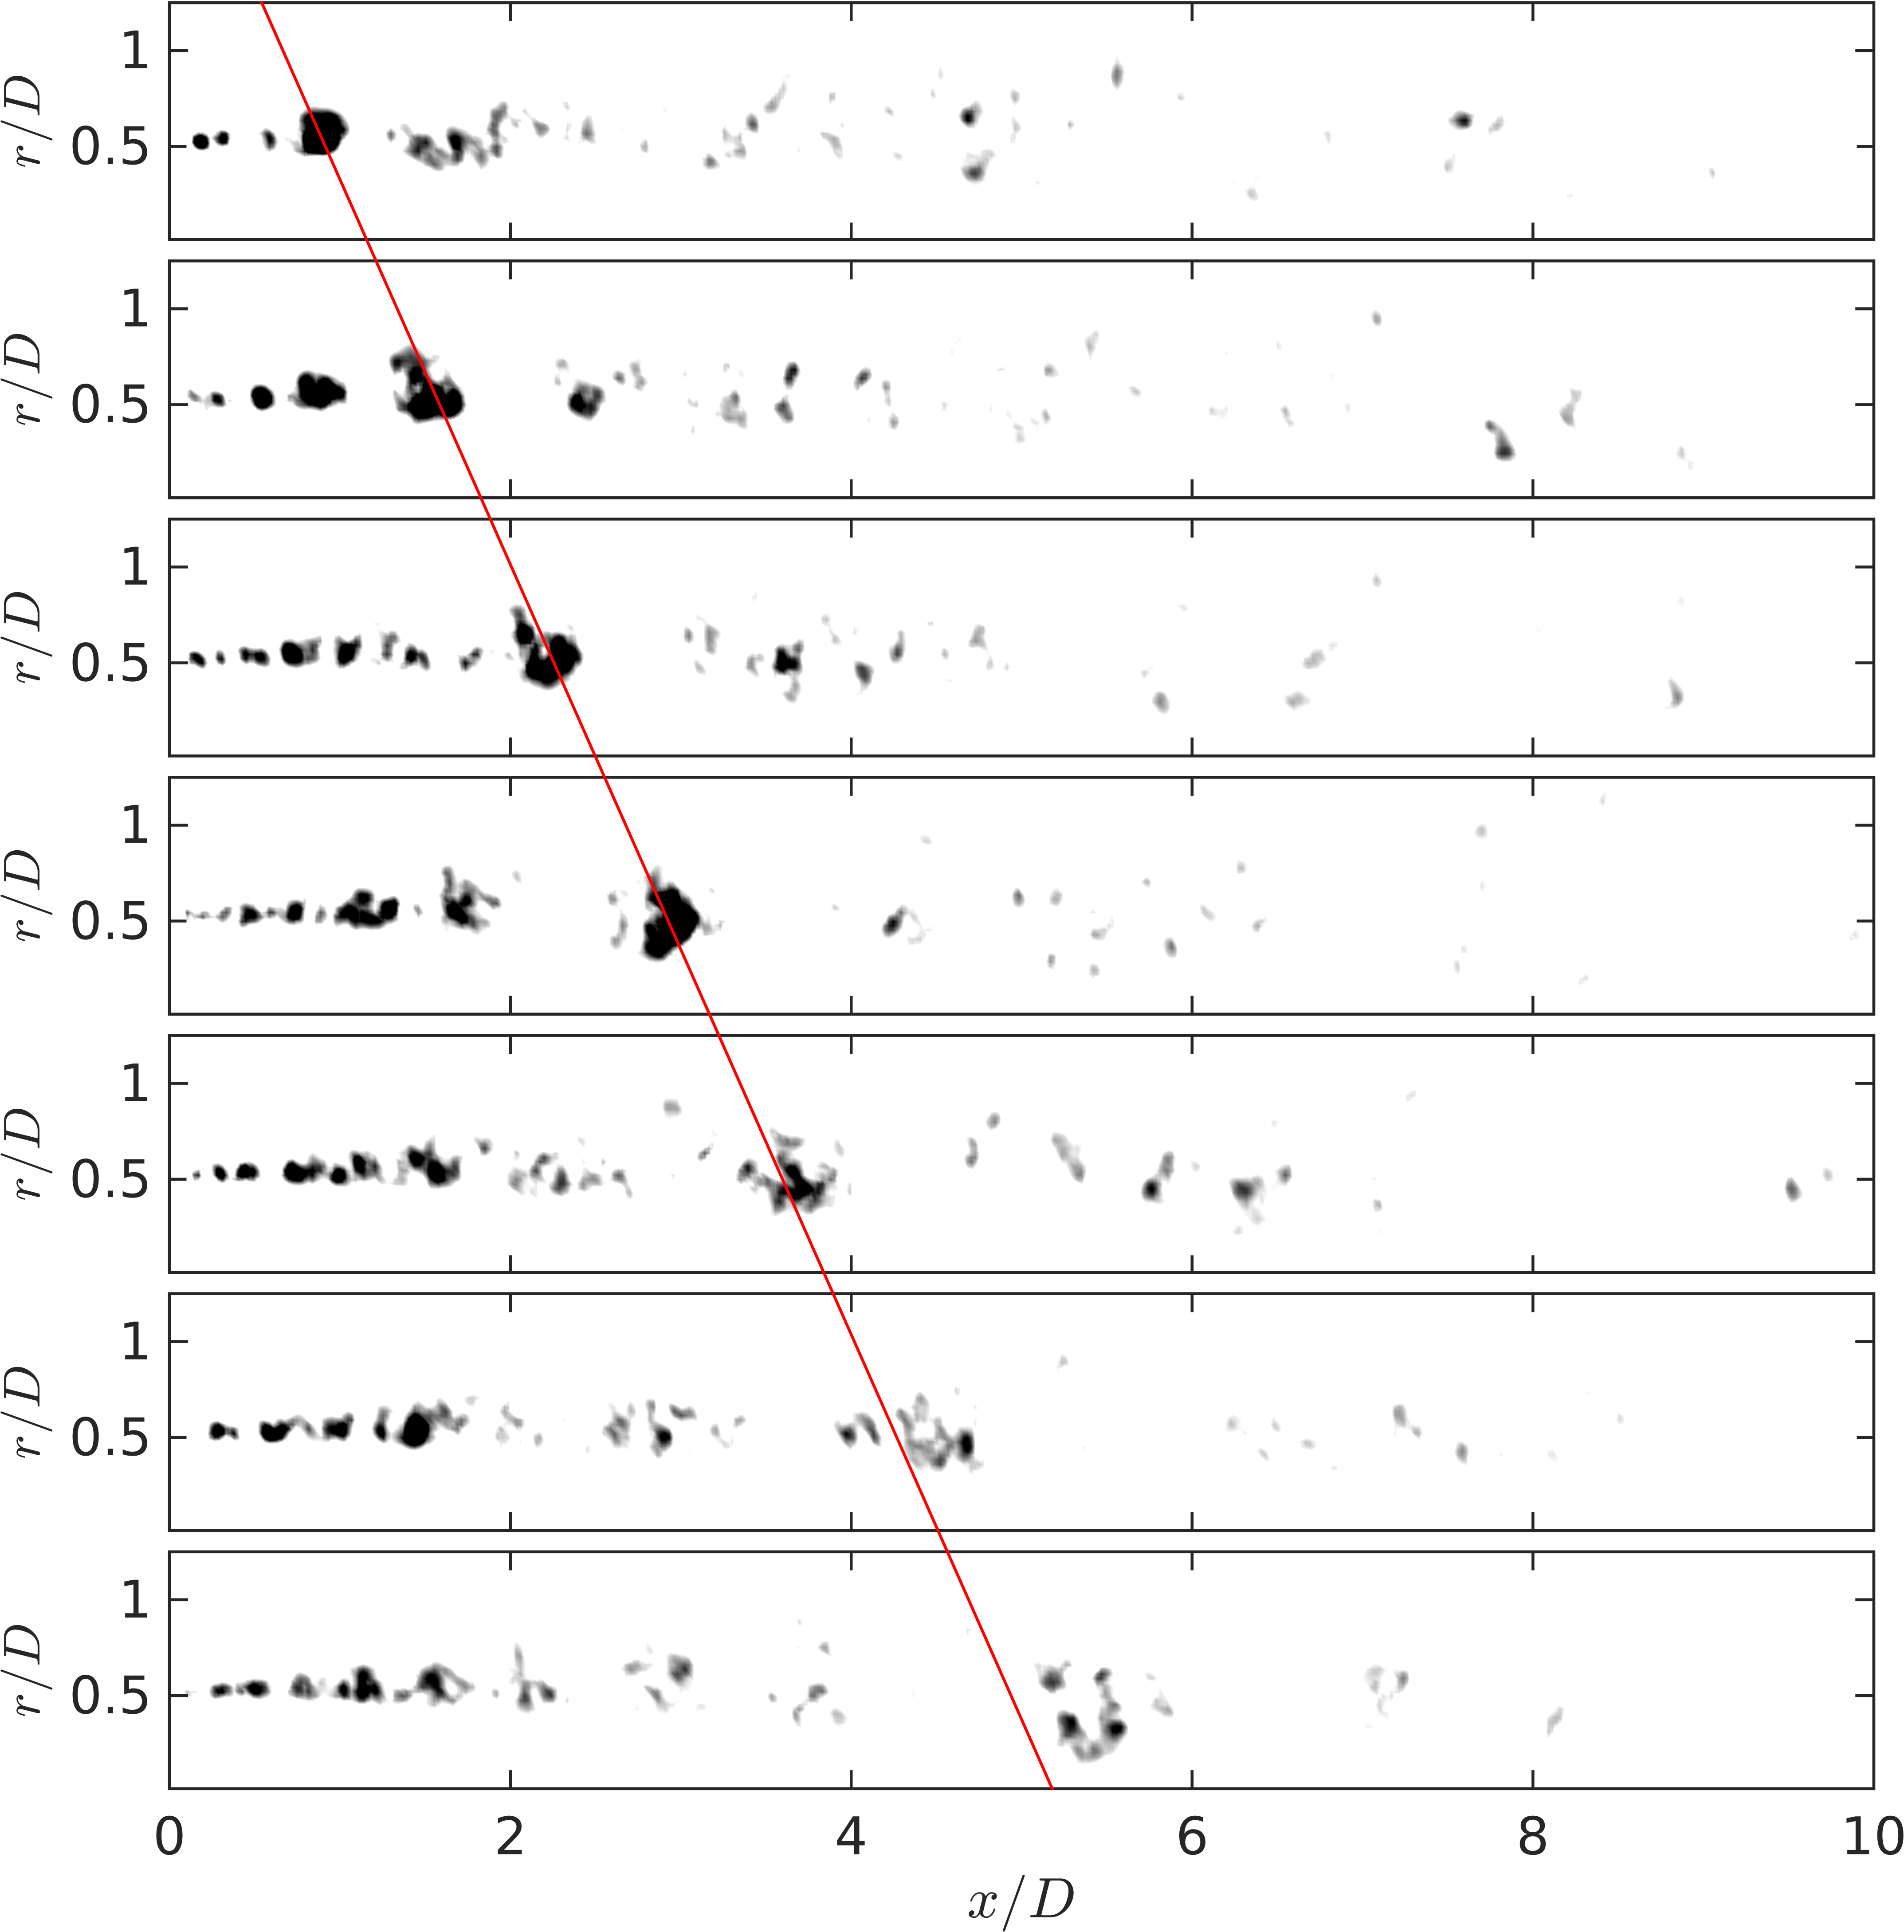
\includegraphics[width=5in]{Figures/ch4_St005_lambda.png}
	\caption{Evolution of the independent vortex ring ($St_{DF}=0.05$), as visualized using swirling strength. Images are shown at constant phase steps of roughly $\pi/8$, starting with a phase of $\pi/4$.}
	\label{fig:ch4_impulse_structure_disintegration}
\end{figure}

As already known from prior experiments at the GDTL \citep{Kearney-Fischer2009}, the excitation produces a strong roll-up of vortical (toroidal) fluid in the near-nozzle region; in the present case the large-scale structure generated by the excitation is clearly discernible over the background turbulence (and experimental/computational noise) by $x/D \simeq 1$.
If the contours of the swirling strength field are to be believed, the rapid growth of the vortex slows by $x/D \simeq 1.5$ and it advects downstream relatively unchanged until  $x/D \simeq 4$ (other vortex identification methods, such as Q-criterion or $\lambda_2$-criterion, were also investigated and a general agreement was found, though swirling strength produced the visually-simplest fields).
It is at this point that the vortex undergoes a rapid disintegration, yielding smaller scale, less coherent structures (though by no means would these structures be classified as fine-scale turbulence) as it passes through the end of the potential core.
These results are in general agreement with those of Hileman \etal \citep{Hileman2005}, who found that the large-amplitude acoustic bursts of energy were associated with the passage of high-order structures through the end of the potential core.
\begin{figure}
	\centering
	\begin{subfigure}{1\textwidth}
		\centering
		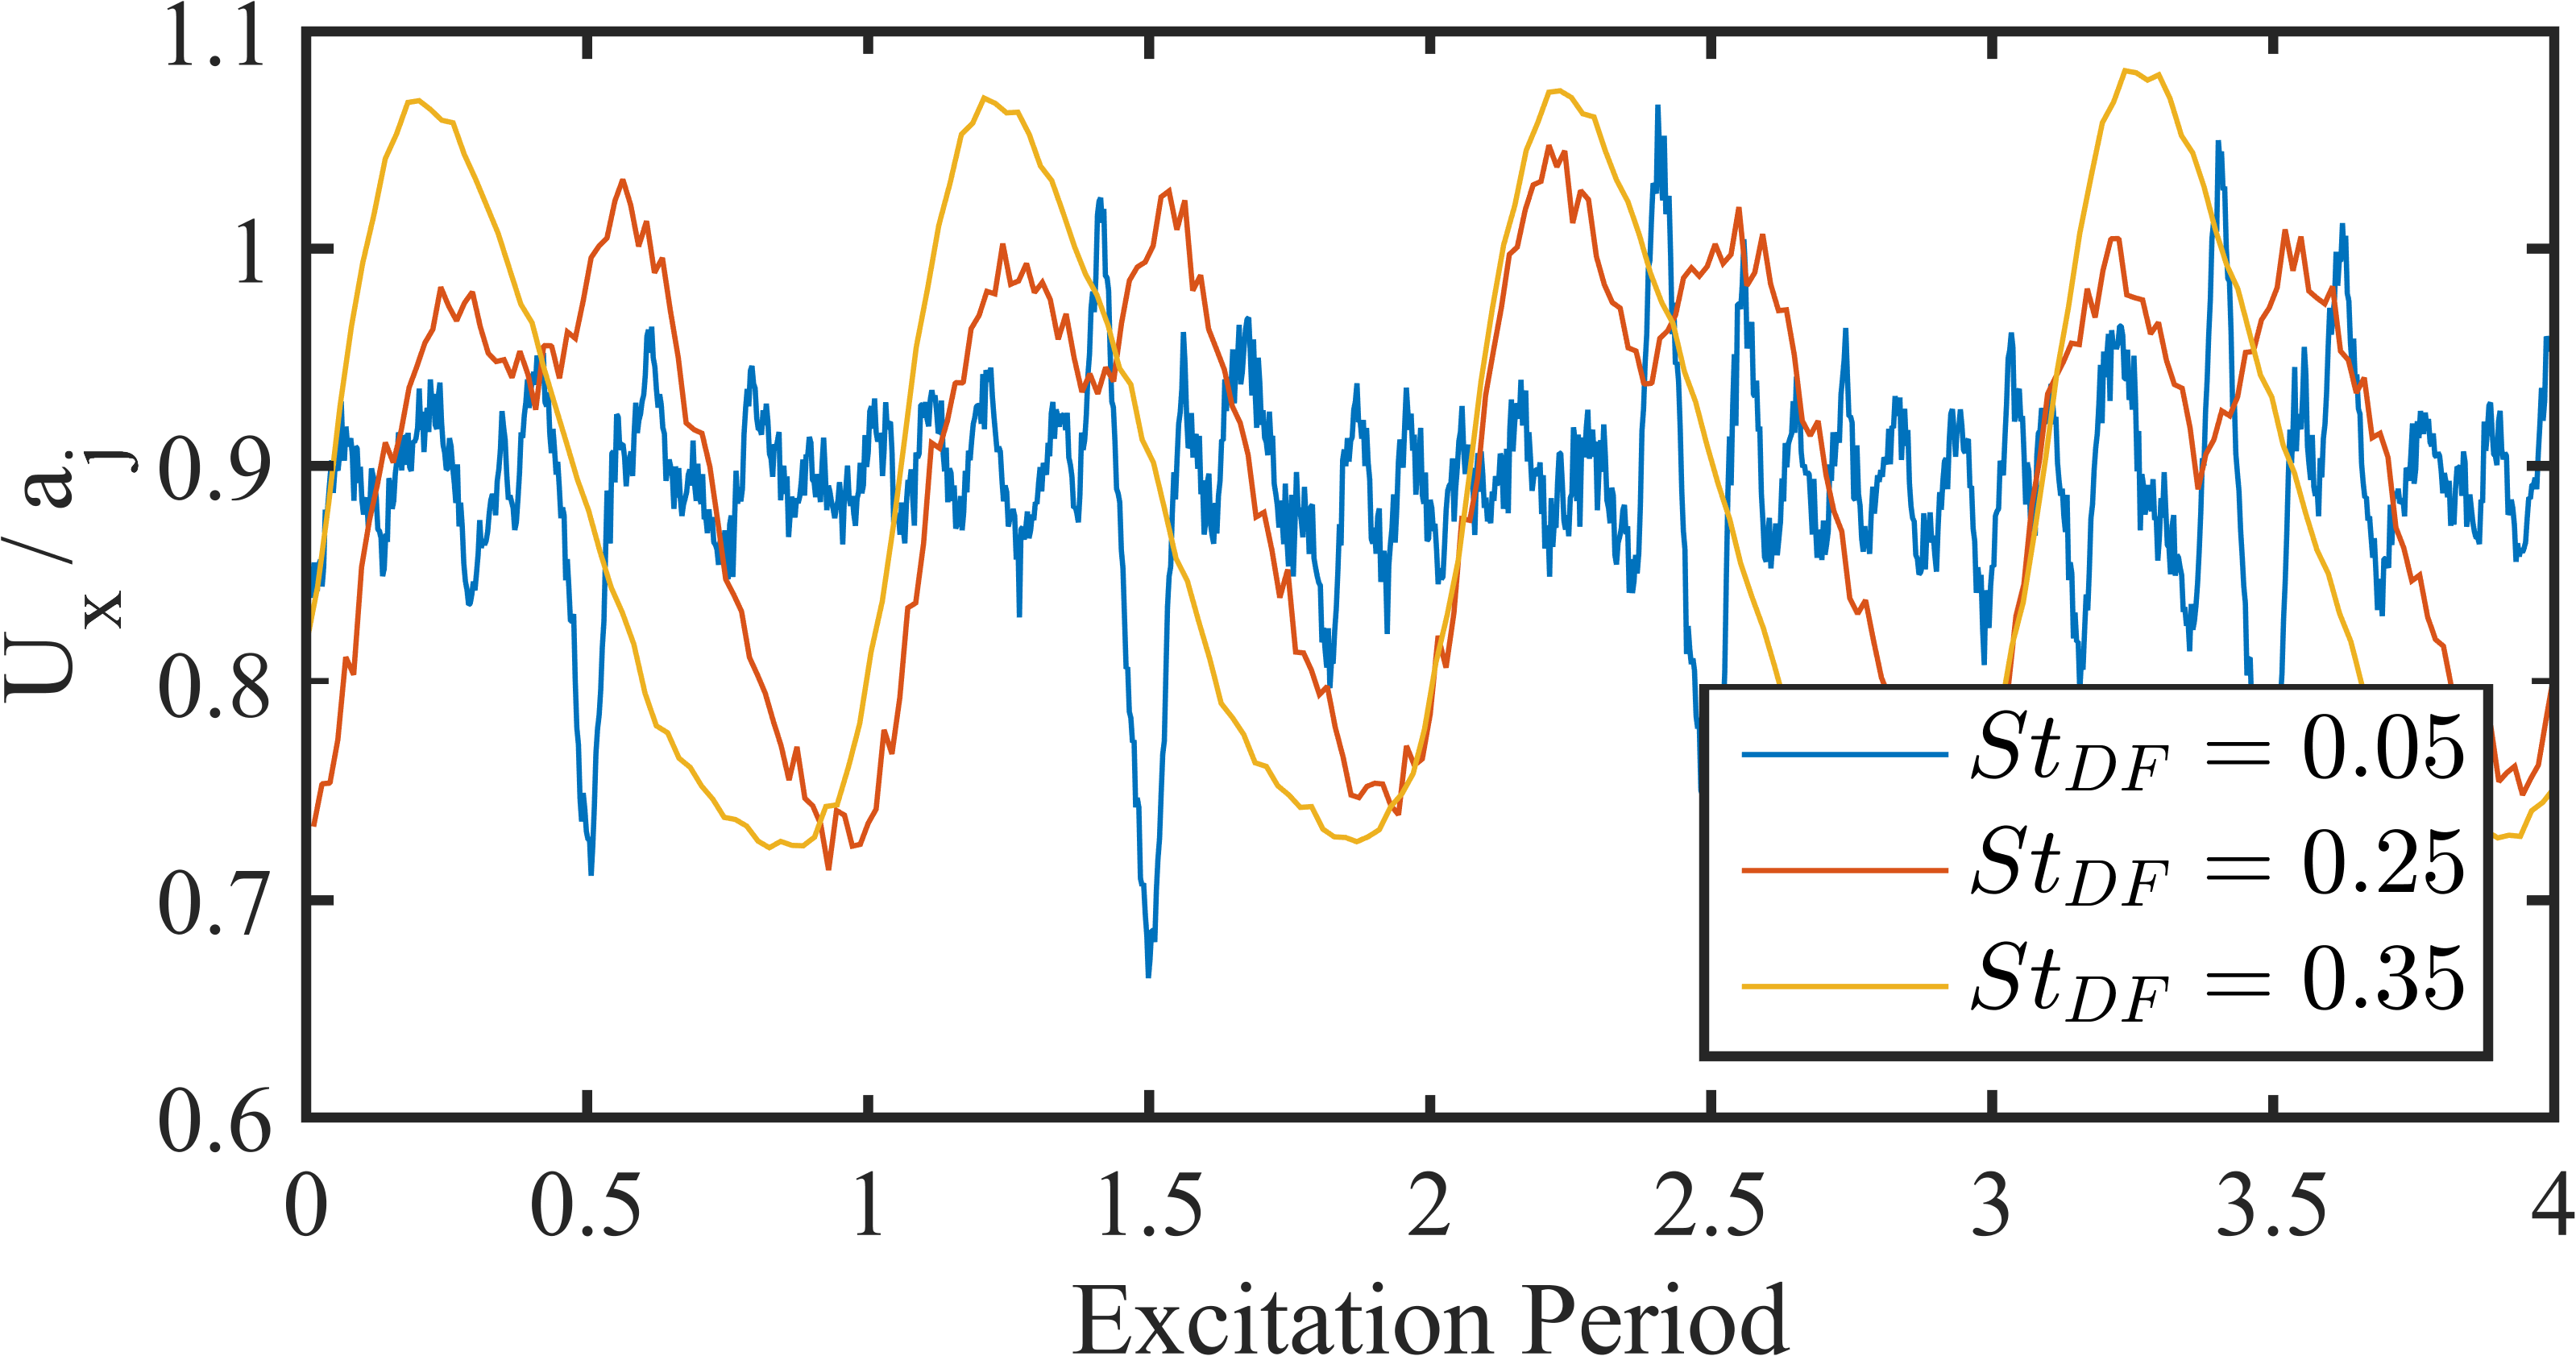
\includegraphics[width=3.5in]{Figures/ch4_centerline_mach_temporal.png}
		\caption{}
		\label{fig:ch4_centerlinemach_temporal}
	\end{subfigure}\\
	\begin{subfigure}{1\textwidth}
		\centering
		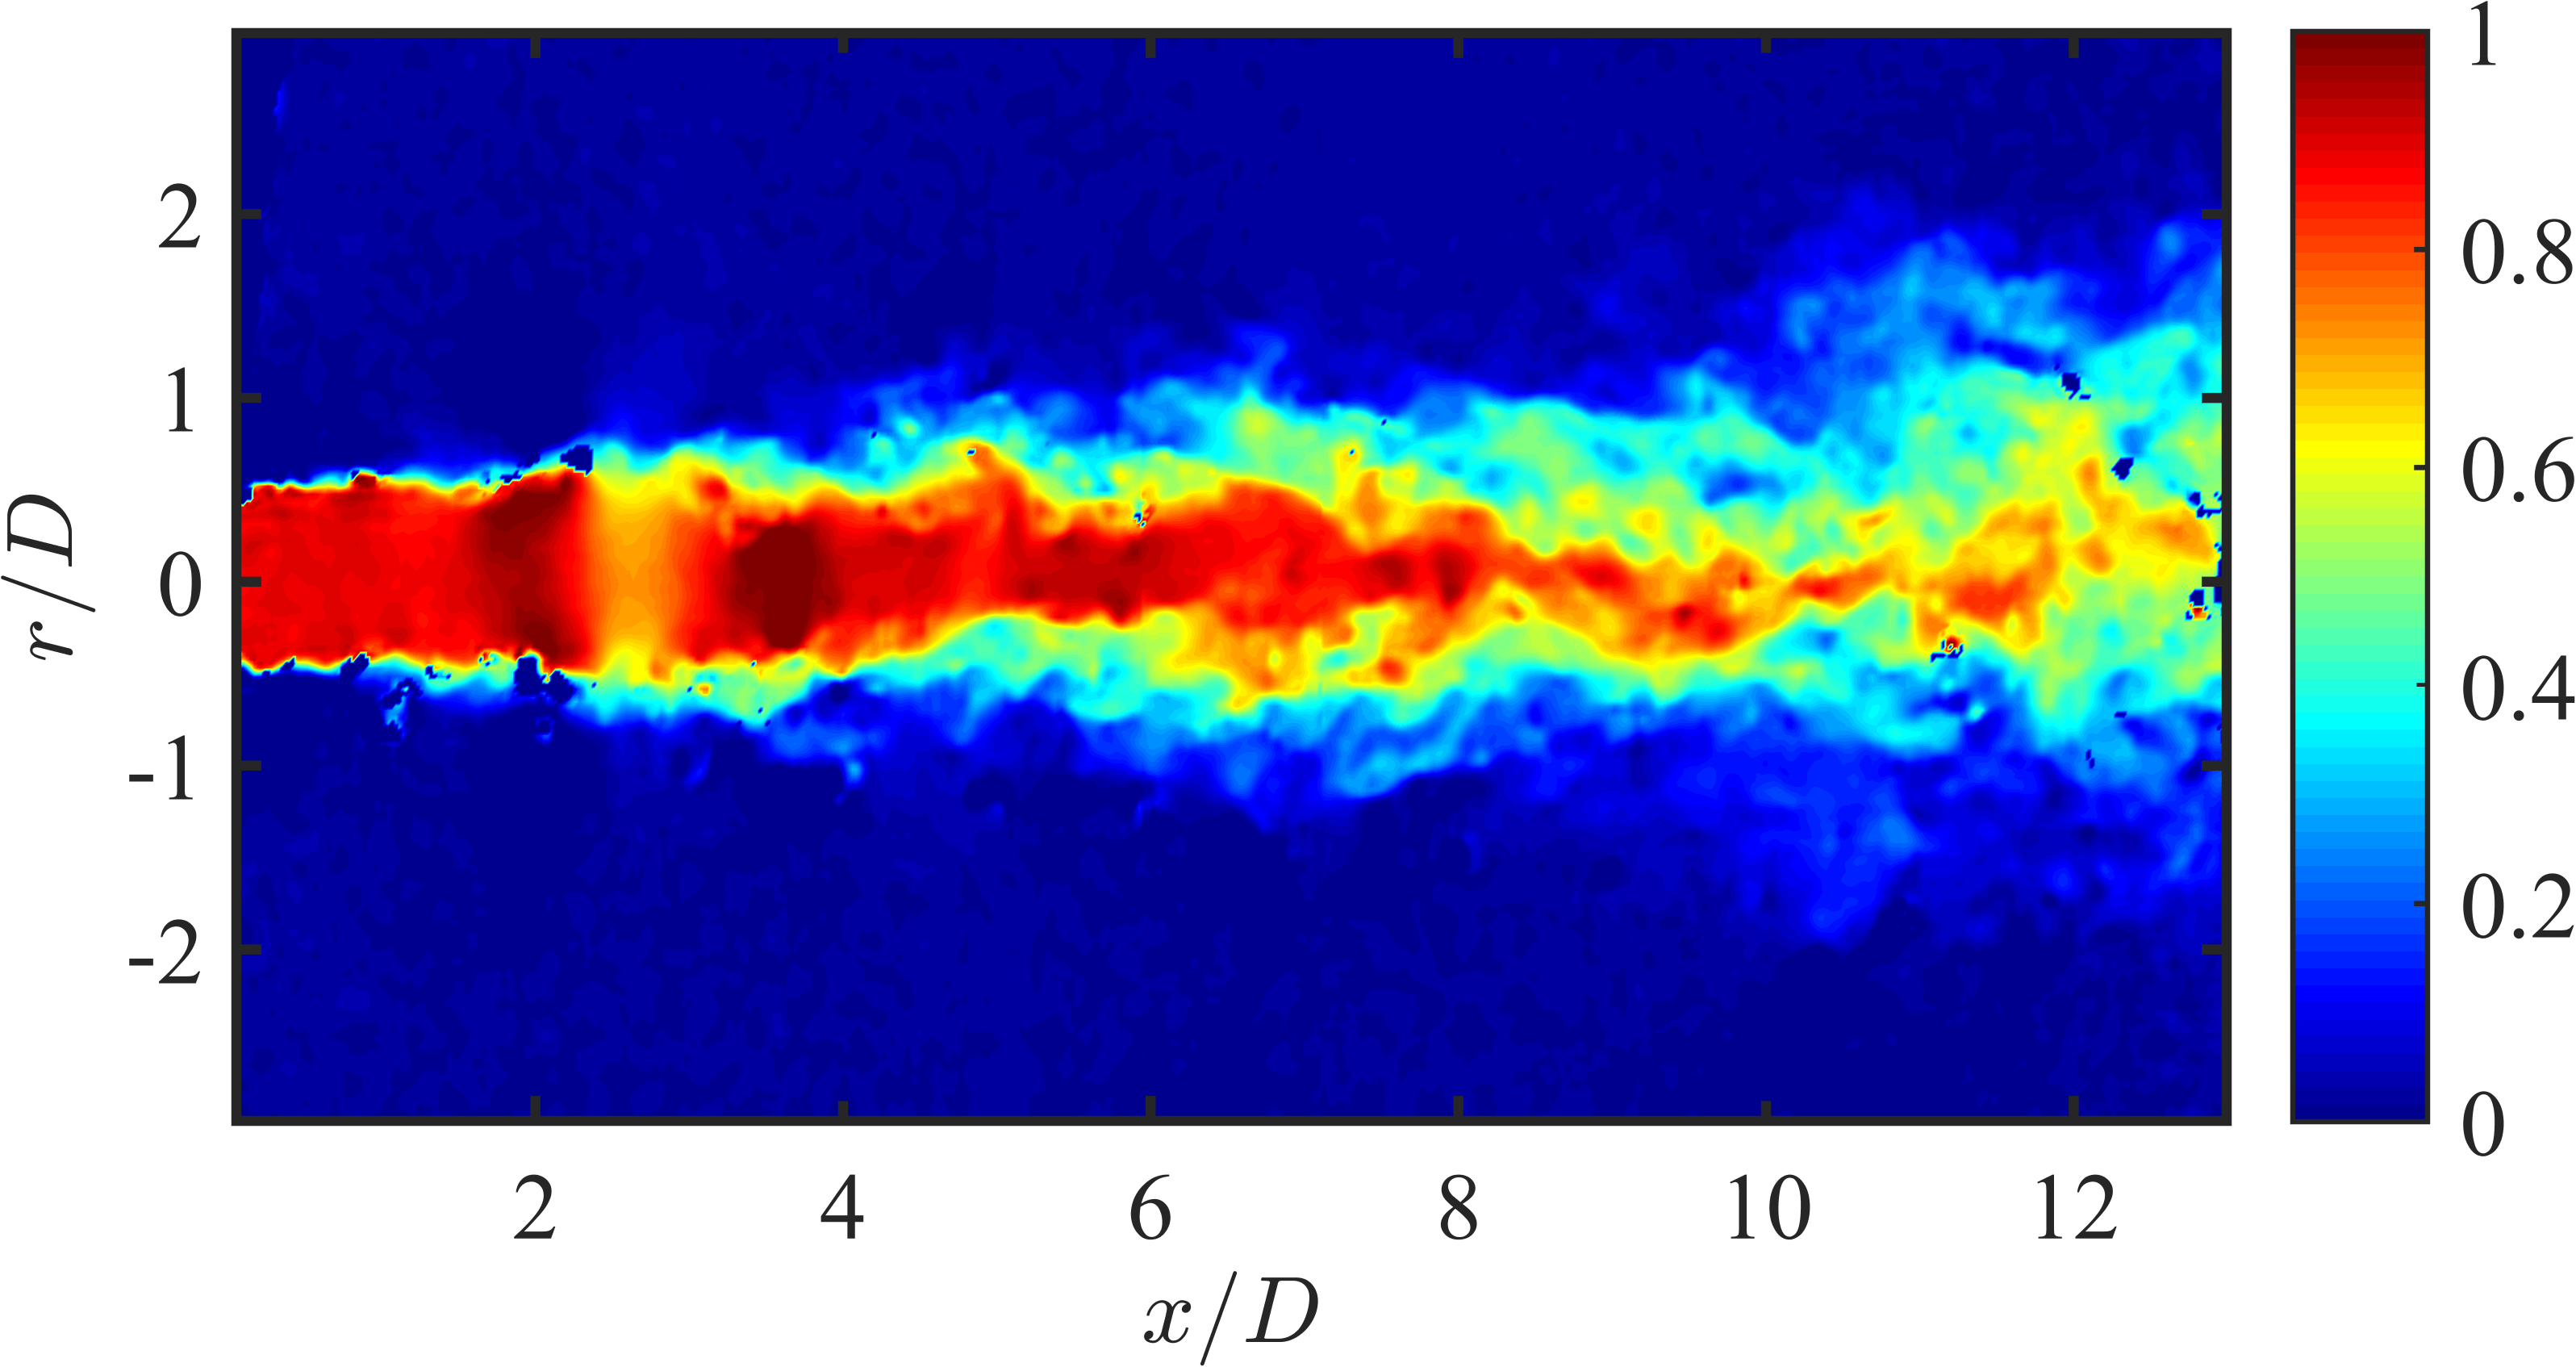
\includegraphics[width=3.5in]{Figures/ch4_rawUx_acceleration.png}
		\caption{}
		\label{fig:ch4_St005_rawUx_snapshot}
	\end{subfigure}
	\caption{Fluctuations associated with the passage of large-scale structures in the axial velocity along the jet centerline at $x/D = 4$ (a) and an arbitrary raw PIV snapshot displaying similar behavior for the $St_{DF}  = 0.05$ jet(b).}
\end{figure}

Accompanying the passage of the vortical structure is a large amplitude oscillation in the axial velocity, which reaches into the potential core to the jet centerline (which is expected, given the radial profile of axisymmetric instability waves known from linear stability analysis \citep{Michalke1965}).
As shown in \fig{fig:ch4_centerlinemach_temporal}, the vortical structures are characterized by large velocity deficit, which is preceded by a large acceleration of the fluid that often crosses the sonic threshold as the vortex begins to disintegrate.
The author was surprised to see such a strong axial acceleration, however this same axial acceleration can also be found in the raw PIV snapshots that have not been post-processed by SE-POD if one looks for it (note the coherent region of supersonic velocity just upstream of $x/D = 4$ in \fig{fig:ch4_St005_rawUx_snapshot}).
An acceleration of the less-coherent structures can also be observed in \fig{fig:ch4_impulse_structure_disintegration}, as the small eddies are located further downstream in the final frames than they would be if following a constant convective velocity (as denoted by the red line overlain on the frames).
As discussed by Tam \citep{Tam1996} (among others), the aeroacoustic efficiency of structures increases with Mach number and envelope modulation.
Therefore, the twin effects of rapid disintegration (\ie rapid envelope modulation) and acceleration around $x/D \simeq 4$ would to greatly enhance the acoustic efficiency from the vortex.
This potentially explains why the region in which the turbulent structure rapidly disintegrates appears to dominate over the region in which the turbulent structure rapidly grows in terms of the noise emission per the results of \sect{sect:nearfield}.

\subsection{Coherent Structure Merging}
In the simulated subsonic shear layer of Wei \& Freund \citep{Wei2006}, optimized control for noise mitigation using generalized actuation was implemented using the adjoint perturbation method.
The methodology was able to affect a significant reduction in the emitted noise, though the exact mechanism by which this was accomplished was not immediately clear, even in this highly simplified flow (two-dimensional shear layer).
In Cavalieri \etal \cite{Cavalieri2010b} the same numerical database was investigated with a specific focus on identifying intermittent events related to the noise generation process.
Here it was found that the control achieved the majority of the sound reduction by suppressing a single triple vortex interaction, thereby regularizing the flow and preventing the generation of high-amplitude peaks in the acoustic field.
The results of Bridges \& Hussain \citep{Bridges1992} and Kibens \citep{Kibens1980} also identified vortex merging as a prominent noise source in a (low) subsonic jet.
With this in mind, the evolution of the vortices in the periodically excited jets was analyzed.

\fig{fig:ch4_period_structure_disintegration} illustrates a complete excitation period for the $St_{DF} = 0.25$ excited jet; as before the velocity fields were smoothed prior to computation of the swirling strength, and the results have been phase-averaged.
Previous analysis of the near-field had used two-point correlations between subsequent microphones in order to estimate the convective velocity of the large-scale structures; based on the time-lag for the maximum correlation value, the convective velocity was estimated as $U_c \simeq 0.7 U_j$.
However, the analysis of Speth \citep{Speth2015} in a simulated Mach 0.9 unheated jet found that this method over-predicted the convective velocity; for example, near the end of the potential core two-point correlations in the irrotational near-field produced an estimate of $U_c \simeq 0.67 U_j$ whereas correlations in the \textit{flow}-field produced an estimate of $U_c \simeq 0.64 U_j$.
Essentially, the energy of the acoustic field in the irrotational near-field though small, is non-trivial, and as a result the much higher propagation velocity for the acoustic energy skews the convective velocity estimate to slightly higher values.
By using only the hydrodynamic component of the near-field (produced by the decomposition of \sect{sect:ac_decomp}), the convective velocity was estimated as $U_c \simeq 0.54 U_j$ near the nozzle exit and $U_c \simeq 0.65 U_j$ near the end of the potential core (which, incidentally, are nearly identical to the values reported in Speth \citep{Speth2015}).
Based on these values, the vortex spacing is expected to range from $\lambda \simeq 2.3D$ at the nozzle exit to $\simeq 2.6D$ near the end of the potential core.
\begin{figure}
	\centering
	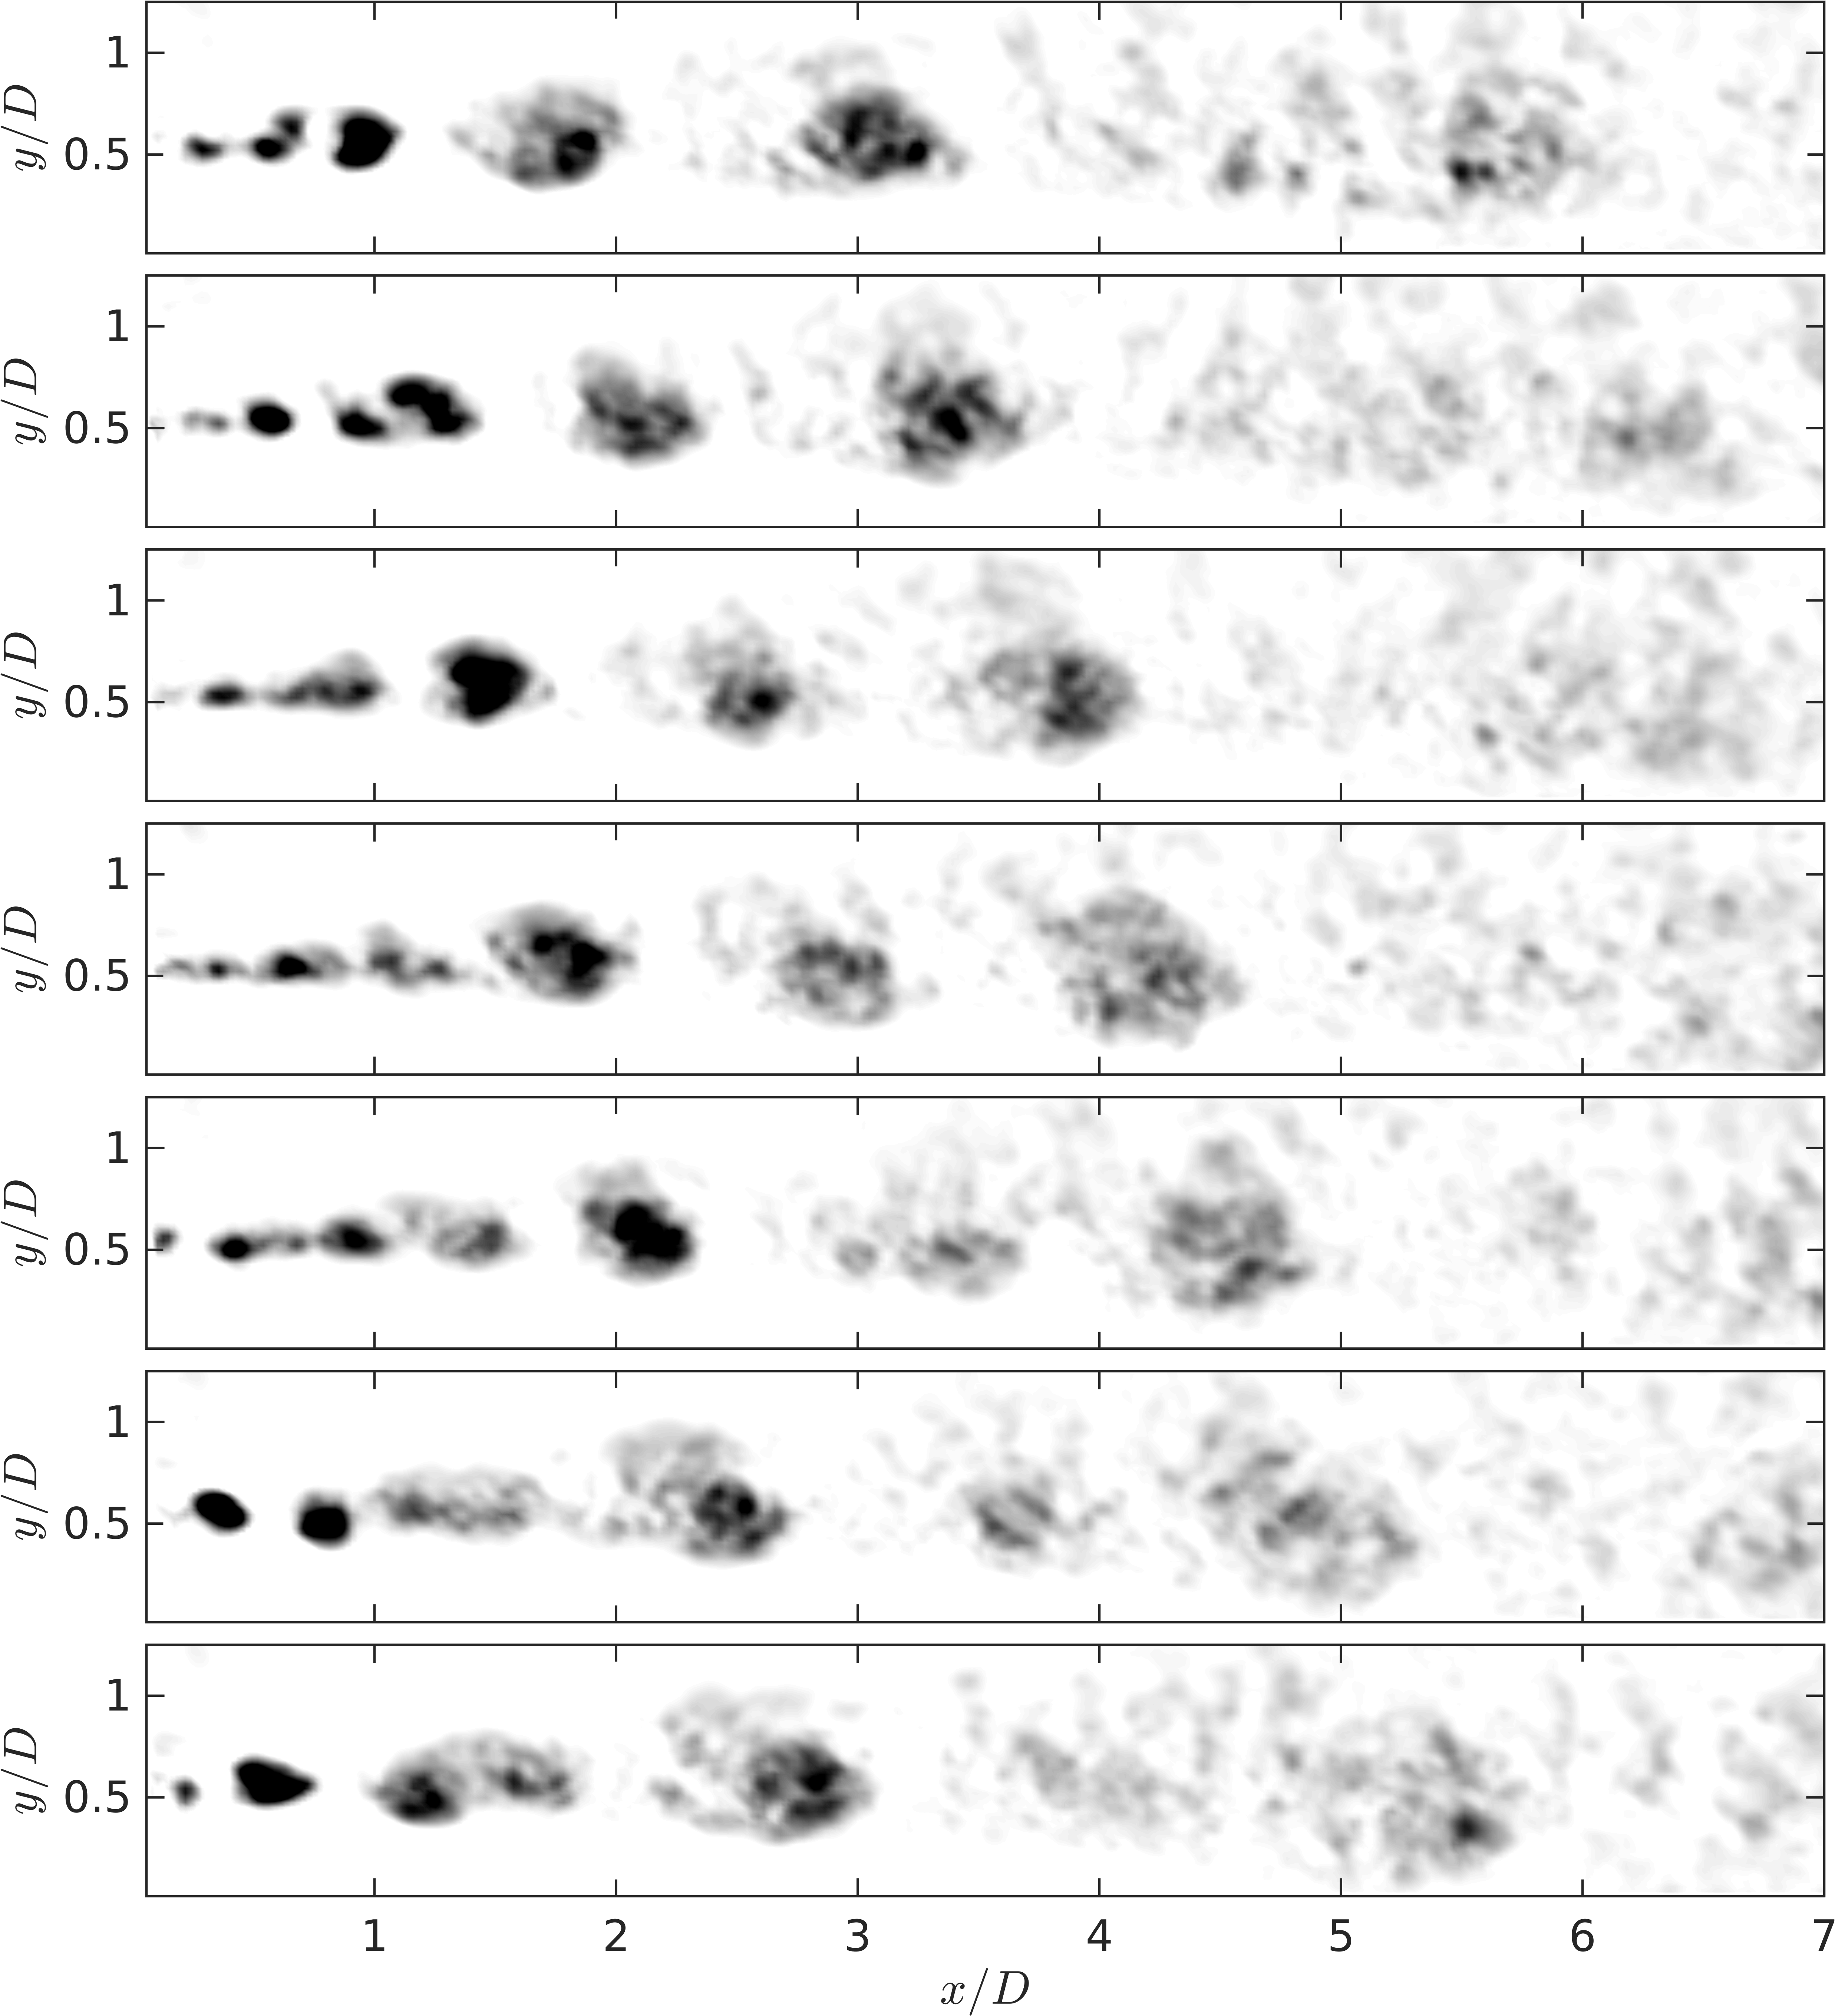
\includegraphics[width=5in]{Figures/ch4_St025_lambda.png}
	\caption{Evolution of the periodic vortex ring ($St_{DF}=0.25$), as visualized using swirling strength. One complete actuation period is shown.}
	\label{fig:ch4_period_structure_disintegration}
\end{figure}

As expected, the excitation produces a periodic roll-up of large-scale structures which, in the downstream region of the potential core, roughly match with the vortex spacing for this frequency (see frame 1 in \fig{fig:ch4_period_structure_disintegration}).
However, in the upstream region ($x/D < 2$) the vortex spacing halves - the LAFPA excitation is in fact producing multiple structures per actuation pulse.
In frame 2, the harmonic structures at $x/D = 1$ are beginning to merge.
The trailing structure is inducted inside the preceding structure, and by $x/D \simeq 3$ the merging process is complete; the appearance of structures now matches the excitation frequency.
The physical interpretation of POD mode 10 in \fig{fig:ch4_St025_PODmodes} is now obvious: the orthogonal decomposition is identifying the harmonic structures and their coherent merging in the upstream region of the jet.
As the resultant structure convects downstream, the beginning of the breakdown of the vortex is witnessed near $x/D \simeq 4$, similar to the results of the impulsively excited vortex ring and an acceleration of the centerline velocity to slightly supersonic speeds is also observed (\fig{fig:ch4_centerlinemach_temporal}).
Here however, a secondary interaction between structures appears to be occurring, most visibly in frames 5--7. 
As the vortex at $x/D \simeq 4.5$ is breaking down, the trailing vortex does as well, in fact much more abruptly than the leading vortex.
As the cycle is repeated (beginning again at frame 1), these two vortices (or more accurately, the less coherent, higher-order remnants of them) are no longer individually distinguishable.

On the other hand, the far-field response of the jet to periodic excitation at $St_{DF}=0.35$ could not be reproduced accurately using a linear superposition of the impulse response.
The vortex dynamics that this excitation frequency produces may thus serve as an insightful contrast for understanding the noise generation phenomena.
A complete excitation cycle for $St_{DF}=0.35$ has been visualized in \fig{fig:ch4_St035_structure_disintegration}.
In this case, two merging processes are now clearly evident.
The first begins just downstream of the nozzle exit, and completes by $x/D \simeq 1.5$; the second begins at $x/D \simeq 2$ and completes relatively quickly, at $x/D \simeq 3$.
It is after this second merging process that the structure spacing now matches the expected wavelength for this excitation frequency ($\lambda \simeq 1.75D$).
As with the lower frequency excitation cases just examined, the dominant vortex (which matches the excitation frequency) undergoes a disintegration beginning around $x/D \simeq 4$.
What is particularly noteworthy here though, is that the disintegration is more rapid for the $St_{DF}=0.05$ and $0.25$ cases than the $St_{DF}=0.35$ case.
In this case, the coherent structure, though severely weakened, is distinguishable over the background noise even downstream of $x/D = 6$.
As with the other excitation frequencies, the core fluid accelerates to supersonic velocities as the large-scale structures pass through the end of the potential core.
\begin{figure}
	\centering
	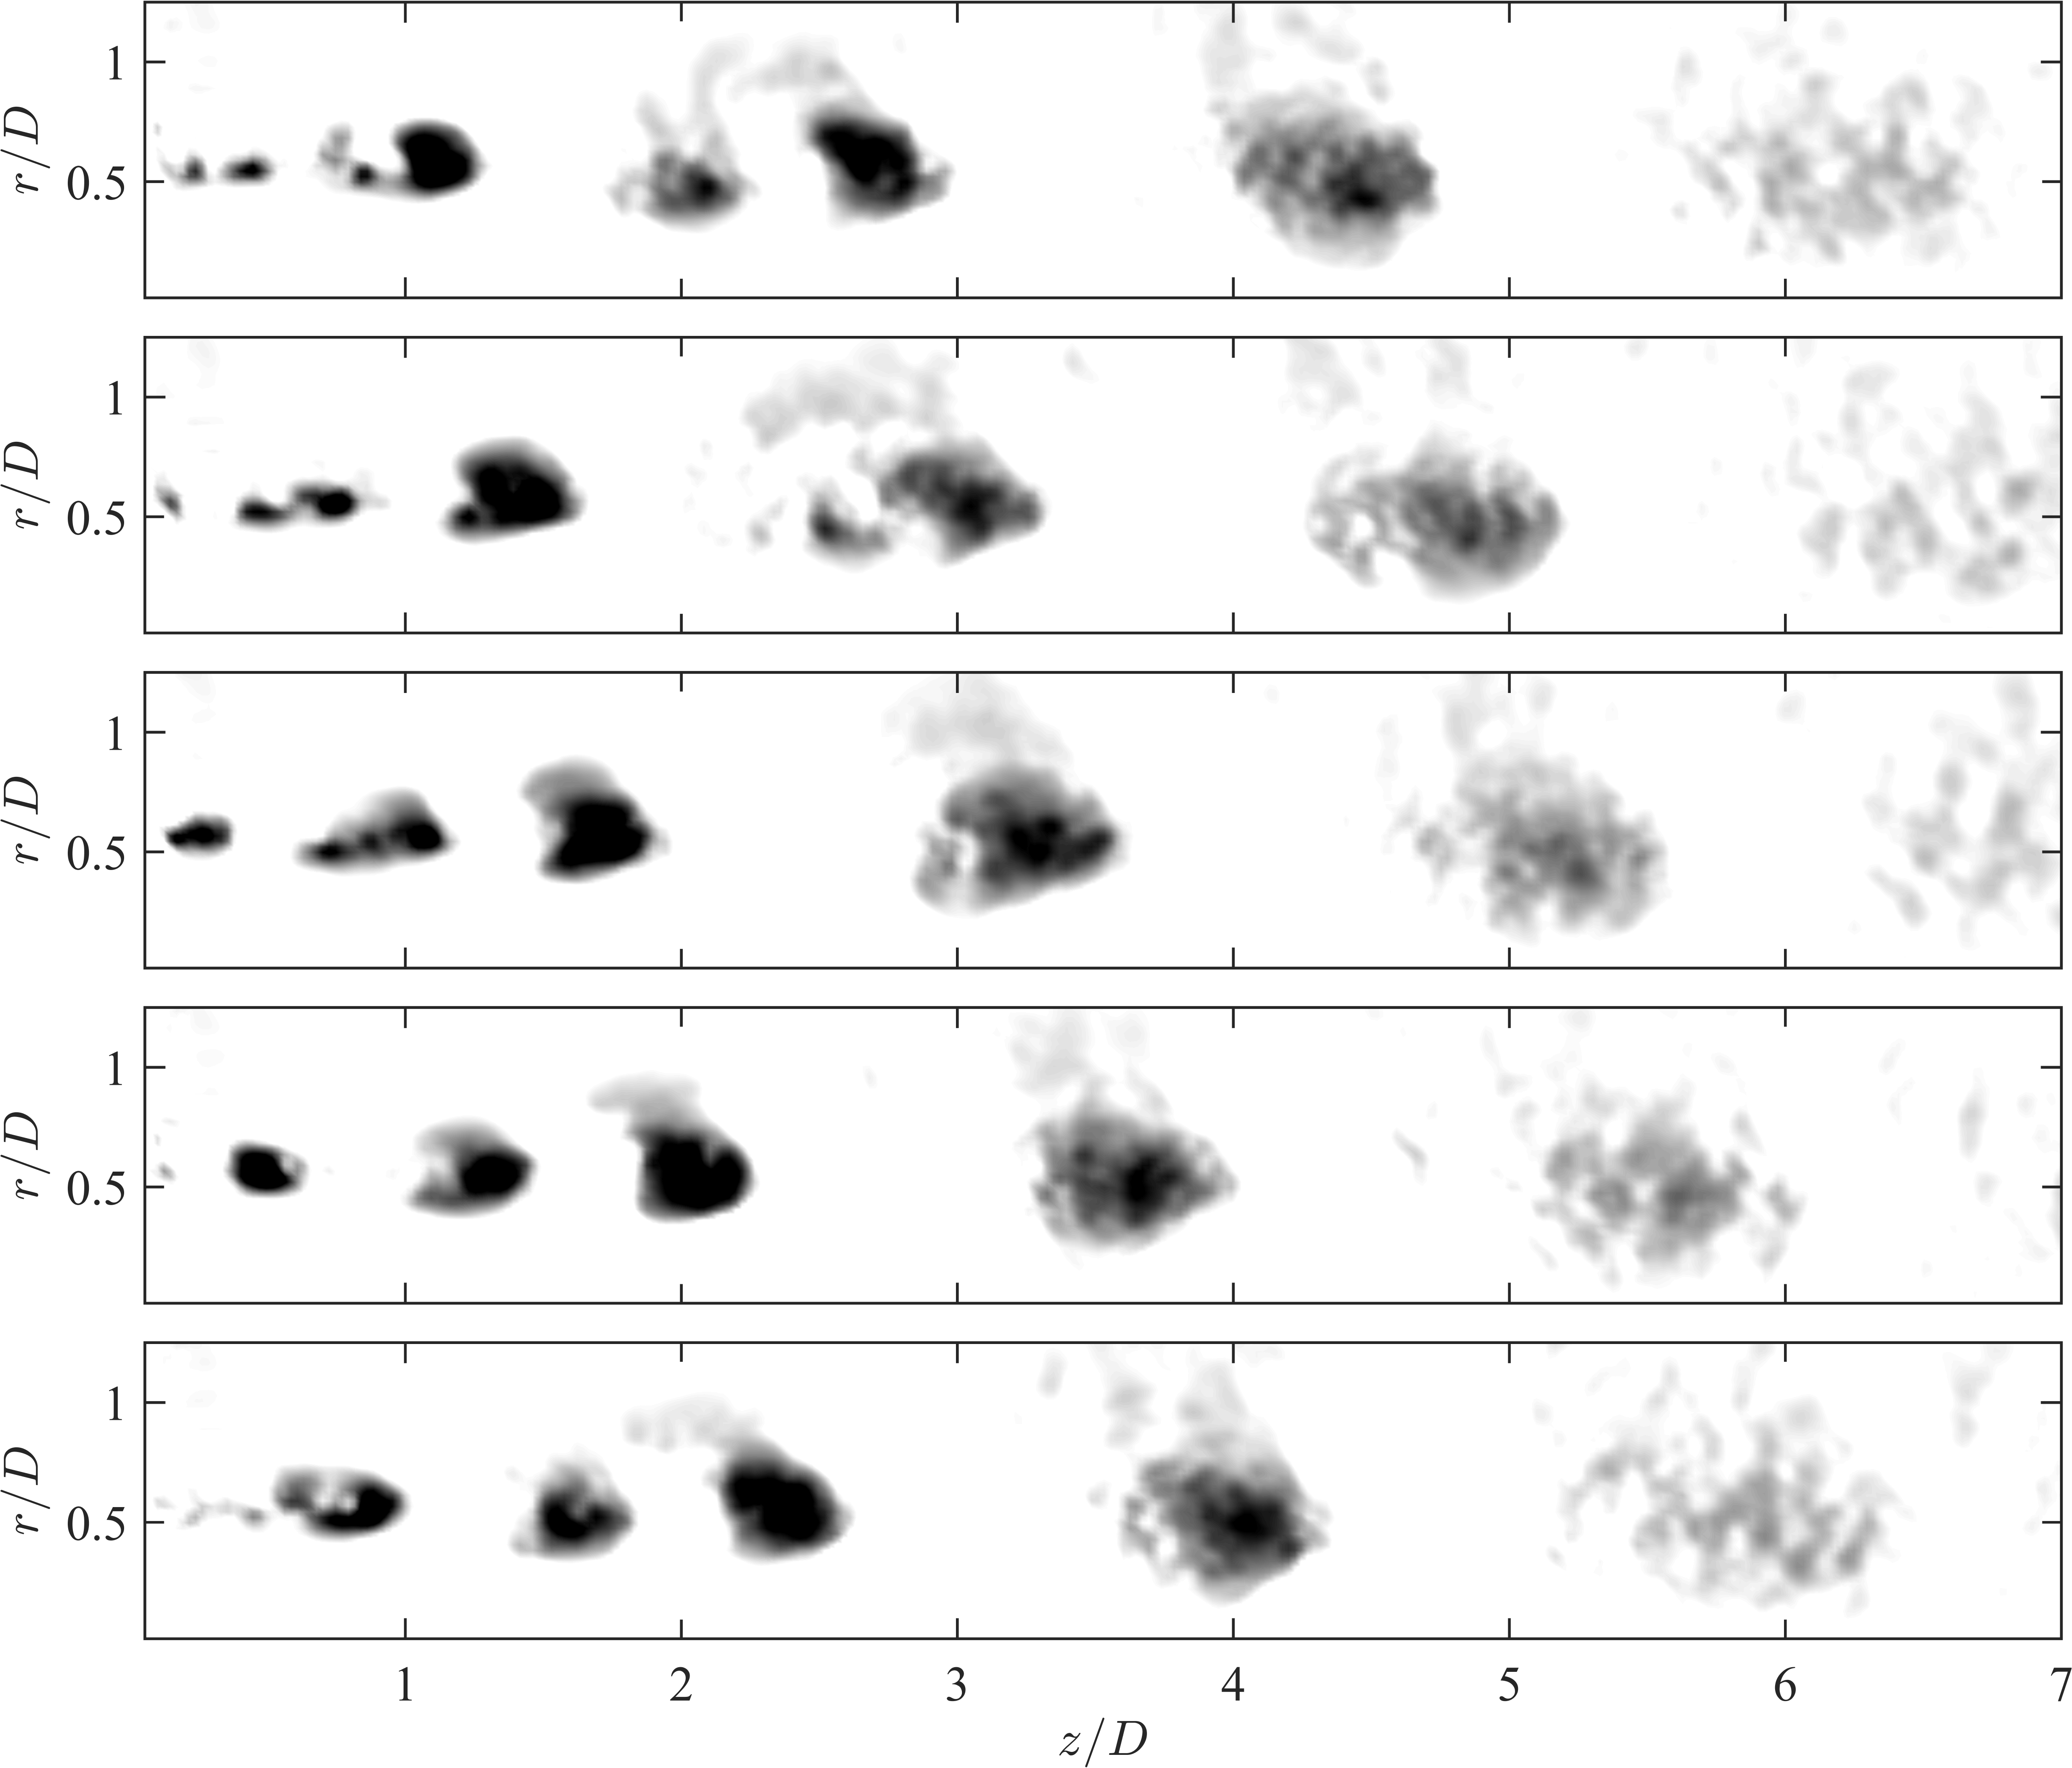
\includegraphics[width=5in]{Figures/ch4_St035_lambda_evolution.png}
	\caption{Evolution of the periodic vortex ring ($St_{DF}=0.35$), as visualized using swirling strength. One complete actuation period is shown.}
	\label{fig:ch4_St035_structure_disintegration}
\end{figure}

Clearly (and unsurprisingly), the vortex interactions in the periodically-excited jets are far more complex than the impulsively excited jet.
However, as was seen both in terms of the far-field response (\fig{fig:ch3_farfield}) as well as the acoustic source region estimated from the decomposed near-field (\fig{fig:ch3_xcorrOA}), the acoustic fields for $St_{DF}=0.05$ and $St_{DF}=0.25$ show remarkable similarity, at least at angles close to the jet axis.
Therefore, this implies that for this excitation range, the added complexity of the periodic excitation (harmonic structures, vortex merging) are not the primary drivers for noise emission (though they may still play a role).
The consistent, rapid breakdown of the LAFPA-induced structures near $x/D \simeq 4$ and accompanying fluid acceleration in both excited jets appears to be the dominant noise source. 
In contrast, the far-field acoustic response to excitation at $St_{DF}=0.35$ is not accurately reproduced by a linear superposition of the impulse response of the jet.
Analysis of the vortex dynamics demonstrates multiple merging processes occurring for this excitation frequency, and though the dominant vortex breaks down at $x/D \simeq 4$, this process is far less dramatic than in the lower-frequency excitation cases.
In this case, the merging process may in fact be a significant factor in the noise generation process.
In order to more conclusively link this behavior to the noise emission directly, in \sect{sect:source} the aeroacoustic source term will be calculated from the estimated time-resolved velocity fields using a simplified form of Lighthill's acoustic analogy.
\chapter{Dilatation as the Aeroacoustic Acoustic Source}
Ribner presented an alternative approach to Lighthill's acoustic analogy which posited fluctuating fluid dilatations as the source of aeroacoustic emission.
\section{Numerical Method}
\subsubsection{Helmholtz Decomposition}
	For a given vector field, $\vec{F}$, Helmholtz's theorem states that any sufficiently smooth vector field can be linearly decomposed into irrotational and solenoidal vector fields, as
	\begin{equation}
	\vec{F} = \vec{F}_{potential} + \vec{F}_{rotational} = \nabla \Phi + \nabla \times \Psi
	\end{equation}
	where $\Phi$ is a scalar field and $\Psi$ is a vector field.
	From basic vector calculus properties, we can therefore compute these solenoidal and irrotational components by taking the divergence of this equation, leading to:
	\begin{equation}
	\nabla \cdot \vec{F} = \nabla^{2} \Phi
	\end{equation}
	which is simply Poisson's equation, where in the context of velocity decomposition the forcing term is simply the divergence of the flow field.
	Since we are unable to acquire gradients in the azimuthal coordinate, we are going to drop this term, leaving
	\begin{equation}
	\frac{\partial U_r}{\partial r} + \frac{\partial U_z}{\partial z} + \frac{U_r}{r} = \frac{1}{r} \frac{\partial \Phi}{\partial r} + \frac{\partial^2 \Phi}{\partial r^2} + \frac{\partial^2 \Phi}{\partial z^2} 
	\end{equation}
	
	The solution procedure is therefore to first compute $\Phi$, then add the gradient of this field to the raw velocity vector field in order to produce the solenoidal velocity field.
\subsubsection{Pseudo-Pressure Solver}
\subsubsection{Wavelet Denoising}
\section{Wavepackets in the Pseudo-Pressure Field}
\chapter{Conclusions}
The aeroacoustic mechanisms in high-speed, turbulent jets were investigated using simultaneous pressure and velocity measurements of large-scale structures generated by plasma excitation.
As the focus of this work was on mixing noise generated by turbulent shear layer structures common to all flow regimes, rather than acoustic emission generated by supersonic flow phenomena, an unheated, Mach 0.9 jet was used.
In the current work, only structures of azimuthal mode zero (axisymmetric ring vortices) were investigated. Previous researchers have identified the axisymmetric mode as the dominant acoustic emission pattern, and this also served to simplify the data acquisition and analysis greatly by eliminating the need to obtain azimuthal velocity components and gradients.

To begin with, the irrotational near-field pressure was linearly decomposed into it's constitutive hydrodynamic and acoustic components, akin to the work of previous researchers \citep{Tinney2008}.
Here though, the pressure was filtered via a two-dimensional, spatio-temporal wavelet transform, which was found to be more robust than the Fourier transform used previously.
Once decomposed, linear correlations between the far-field acoustic signal at $30^\circ$ and the acoustic component of the near-field were computed in order to identify the dominant acoustic source region in the jet based on the measured time-lag for the peak correlation.
In all cases, natural and excited jets, the dominant acoustic source region was found to comprise the upstream region of the jet and end at $z/D \simeq 4$, just upstream of the end of the potential core.
This result is in general accordance with previous results acquired at the GDTL by Hileman \etal \citep{Hileman2005}, which identified the acoustic source region using delay-and-sum beamforming with a circular microphone array in the acoustic near-field (that is, far enough such that hydrodynamic pressure effects are negligible, but not in the true geometric far-field of the jet).
In that work, the dominant acoustic source region for an unheated, Mach 1.3 jet was found to be located just downstream of the end of the potential core, and was related to the breakup of large-scale coherent structures as they passed through this region.

The evolution, interactions, and, disintegration of the large-scale structures induced by the plasma excitation were then studied by stochastically-estimating the time-resolved velocity fields from temporally-correlated velocity snapshots and near-field pressure traces.
The velocity snapshots were first decomposed into orthogonal modes and expansion coefficients per Sirovich's method of snapshots for proper orthogonal decomposition \citep{Sirovich1987}.
A mapping from the near-field pressure to the POD expansion coefficients was generated by a standard feedforward, backpropagating neural network; from this mapping the time-resolved expansion coefficients could be estimated and thus a reduced-order, time-resolved estimate of the velocity field produced.
At very low excitation frequencies (impulsive excitation) each plasma pulse generates a single dominant structure, which initially grows rapidly as it convects downstream. 
As the structure nears the end of the potential core, $z/D \simeq 4$, a rapid disintegration of the vortex is observed, coincident with a strong axial acceleration.
As the excitation frequency is increased, a much more complex structure evolution takes form.
At moderate excitation frequencies (periodic forcing), multiple structures are initially formed by the plasma pulse; these quickly merge to form periodic structures which match the excitation frequency.
These structures later undergo a rapid disintegration and acceleration, similar to the impulsive excitation structures, as the convect downstream near the end of the potential core. 

Finally, the aeroacoustic sources were estimated from the time-resolved velocity fields using Ribner's simplified form of Lighthill's acoustic analogy, which relates fluctuations in the dilatation field to fluctuations in the acoustic field.
This required numerous simplifications to the governing equations, which ultimately degraded the accuracy of the computed aeroacoustic source field.
Unfortunately, this limited interpretation of the results, as the computed far-field acoustic signal did not match well with the measured signal.
It had been hoped that high-resolution velocity fields and nonlinear estimation methods would be sufficient for overcoming the challenges inherent in measuring acoustic source fields in high-speed, turbulent jets, but clearly this was not the case. 
An experimentalist can always dream, though.

% % %What do the final results show????

% %Future work section
Perhaps the greatest deficiency in the current work was the reliance on linear correlations from the acoustic component of the near-field to the far-field.
This was done because two-point correlations are quick, simple, and their use is well-established in the literature.
However, this overlooks the great advancements in acoustic holography that have occurred in the last several decades.
Though the linear array of microphones used in this work is not well-optimized for acoustic beamforming, additional information on the noise source characteristics, such as directivity or frequency content, can likely be gleaned from the decomposed irrotational near-field using a number of beamforming algorithms of varying complexity.
Readers interested in acoustic beamforming are referred to the work of Papamoschou \citep{Papamoschou2011}.

%\appendix

%
% The all important bibliography file at the end of your document!! Use
% the bibstyle you (your department) like in the \bibliographystyle{}
% statement and list the name of your bibliography database file in
% the \bibliography{} statement.  In this example, ``bibfile.bib'' is
% the name of the database.  See the LaTeX manual appendix B for details
% about the bibliography database and BibTeX.
%

\bibliographystyle{plain}
\bibliography{new_master}

\end{document}




